%!TEX root = ../Thesis.tex
\chapter{Fission Source Convergence \label{ch:AdvancedArnoldi}}
Monte Carlo criticality calculations have come a long way since their beginning in the 1950s.  Along with the increase in the speed and complexity of computers the problems for which Monte Carlo techniques have been used have increased.  Problems that were prohibitively expensive in the past have now become routine.  Some problems still remain, however,  with Monte Carlo criticality calculations.  Two of those problems are fission source convergence and the underestimation of the variance of the mean eigenvalue \citep[see][]{Brown:2009A-Rev-0}.  In this chapter we will discuss how a Monte Carlo application of Arnoldi's method improves the source convergence as compared with the traditional power method.

\section{Shannon Entropy and Fission Source Convergence \label{sec:Entropy} }
In \Fref{sec:PowerMethod} it was observed that a Monte Carlo code must discard initial iterations as the eigenvalue estimate converges to the fundamental eigenmode.  The number of iterations required for convergence of the power method to the fundamental depends on the dominance ratio ($\lambda_1/\lambda_0$) for the problem.  Also of concern is the convergence of the fission source.  To obtain good estimates of the fission source---or eigenfunction of the fission-transport operator---the fission source should be converged before tallying begins.

Knowing how many cycles to discard can be a challenge.  One could monitor the eigenvalue estimates to see if they have converged and begin active cycles once convergence has been achieved.  \citet{Brown:2009A-Rev-0} suggests that when the dominance ratio is close to 1, the fundamental eigenvalue will converge sooner than the fission source distribution.  We must, therefore, monitor \emph{both} the convergence of the eigenvalue as well as the convergence of the fission source.  It is clear that convergence in fewer iterations is desired because fewer iterations will have to be discarded and tallying can begin sooner.  

One problem for which source convergence in the power method is problematic is a geometry with multiplying regions separated by large region of a highly-absorbing material.  This is because of the particles born in one multiplying region only a few, rare, neutrons would ever transport through the absorbing region to cause fission in the other multiplying region.  In the power method, the only way in which particles can move from the initial source to a new location is through the scattering that occurs in the application of the fission-transport operator.  The fission source for the next iteration contains only the points at which neutrons induced fission in the previous iteration.

When restarting, Arnoldi's method uses all of the available information about the operator applied to a source to estimate an eigenvector; the power method only uses information from the latest application of the operator to estimate the fundamental eigenvector.  Using all available information makes it possible for the fission source to be converged more quickly.  

To monitor the convergence of the fission source \citet{Ueki:2003Infor-0} have used information theory to calculate the Shannon entropy, $H$, of the fission source.   The Shannon entropy of a spatially discretized fission source $S(x)$ is defined as
\begin{equation}
    H(S(x)) \equiv -\sum_{b=1}^B S_b\log(S_b),
    \label{eq:ShannonEntropy}
\end{equation}
where $B$ is the number of spatial bins and $S_b$ is the number of fission neutrons in bin $b$.  As the calculation proceeds, the Shannon entropy will converge to some value.  The actual value of the Shannon entropy is not important in determining the fission source convergence.  What is important is that it converges to some value.

To calculate the Shannon entropy when using the power method the fission source must be discretized.  This discretization is most easily performed using a first order---or histogram---approximation as described in Equations \eqref{eq:ApproximatedSource}, \eqref{eq:FirstOrderApproximation} and \eqref{eq:ConstantSpaceArnoldiVector}.  The discretization of the fission source will not bias the estimate of the eigenvalue in the power method as it does for Arnoldi's method.  The power method samples from the non-discretized source and only uses the discretized fission source for tallying bins and calculating the Shannon entropy.

In Arnoldi's method, we can't calculate the Shannon entropy of the Arnoldi vectors.  We must, therefore, calculate the Ritz vectors of \A{} and use the fundamental Ritz vector as $S(x)$ in \Fref{eq:ShannonEntropy}.  With the first order approximation to the fission source 
\begin{equation}
	S_b = \int_{x_b}^{x_{b+1}} \left|\Px\right| \dd x.
	\label{eq:SbFirstOrder}
\end{equation}
This is equivalent to calculating the Shannon entropy for the Power method.  When using a second order approximation, 
\begin{equation}
	S_b = \int_{x_b}^{x_{b+1}} \left|\Lx\right| \dd x.
	\label{eq:SbSecondOrder}
\end{equation}
In both \Fref{eq:SbFirstOrder} and \Fref{eq:SbSecondOrder} $S_b$ is the number of neutrons that have tallied in bin $b$.


\section{Numerical Results}
\subsubsection{Homogeneous Slab}
To demonstrate the eigenvalue and fission source convergence both the power method and Arnoldi's method have been run on a homogeneous slab, 50 mfp thick with \mbox{$\nu\Sigma_f = 1.0$}, \mbox{$\Sigma_a = 0.2$}, and \mbox{$\Sigma_s = 0.8$}; \mbox{$\Sigma_t = 1.0$}.  This geometry is the same as in \Fref{ch:RelaxedArnoldi}.  Arnoldi's method has 25 iterations per restart and both methods track 5E5 particles per iteration.  The dominance ratio for this problem as estimated by Arnoldi's method is 0.992201.  For this problem I have used a second order approximation to the fission source as described in \Fref{ch:SpatialDiscretization}.

In \Fref{fig:50mfpPower} I show the eigenvalue estimates (red) and Shannon entropy convergence (blue) from the power method.  The solid black line shows the reference value of 0.997520 from a deterministic S$32$ code with 200 equally-spaced regions. The dashed black line shows the entropy at the end of the simulation.  \Fref{fig:50mfpArnoldi} shows the eigenvalue estimate and Shannon entropy convergence as calculated by Arnoldi's method.  In this figure, the dashed black line is the mean value of the Shannon entropy.  

From \Fref{fig:50mfpPower} and \Fref{fig:50mfpArnoldi}, we see that Arnoldi's method converges immediately for both the eigenvalue estimate and the fission source.  The power method, however, requires approximately 250 iterations to converge.  We do see something different in these figures that we did not see before.  In Figures \ref{fig:SymmetricPower}--\ref{fig:AsymmetricArnoldi}, it appears that the spread in the eigenvalue estimates was approximately the same between Arnoldi's method and the power method.  For the homogeneous slab, however, the spread in the eigenvalue estimates from the power method is 0.00052 while the spread from Arnoldi's method is approximately 0.0012---the eigenvalue estimates from Arnoldi's method are less noisy than the estimates from the power method.

Thus we see that Arnoldi's method is superior to the power method for eigenvalue and fission source convergence, both converge immediately.  The eigenvalue estimates from Arnoldi's method are also less noisy that those from the power method.

\begin{figure}[p]\centering
    \subfloat[Power method.]{\label{fig:50mfpPower}% GNUPLOT: LaTeX picture with Postscript
\begingroup%
\makeatletter%
\newcommand{\GNUPLOTspecial}{%
  \@sanitize\catcode`\%=14\relax\special}%
\setlength{\unitlength}{0.0500bp}%
\begin{picture}(8640,5760)(0,0)%
  {\GNUPLOTspecial{"
%!PS-Adobe-2.0 EPSF-2.0
%%Title: 50mfpPower.tex
%%Creator: gnuplot 4.3 patchlevel 0
%%CreationDate: Sat Aug  1 02:43:44 2009
%%DocumentFonts: 
%%BoundingBox: 0 0 432 288
%%EndComments
%%BeginProlog
/gnudict 256 dict def
gnudict begin
%
% The following true/false flags may be edited by hand if desired.
% The unit line width and grayscale image gamma correction may also be changed.
%
/Color true def
/Blacktext true def
/Solid false def
/Dashlength 1 def
/Landscape false def
/Level1 false def
/Rounded false def
/ClipToBoundingBox false def
/TransparentPatterns false def
/gnulinewidth 5.000 def
/userlinewidth gnulinewidth def
/Gamma 1.0 def
%
/vshift -66 def
/dl1 {
  10.0 Dashlength mul mul
  Rounded { currentlinewidth 0.75 mul sub dup 0 le { pop 0.01 } if } if
} def
/dl2 {
  10.0 Dashlength mul mul
  Rounded { currentlinewidth 0.75 mul add } if
} def
/hpt_ 31.5 def
/vpt_ 31.5 def
/hpt hpt_ def
/vpt vpt_ def
Level1 {} {
/SDict 10 dict def
systemdict /pdfmark known not {
  userdict /pdfmark systemdict /cleartomark get put
} if
SDict begin [
  /Title (50mfpPower.tex)
  /Subject (gnuplot plot)
  /Creator (gnuplot 4.3 patchlevel 0)
  /Author (Jeremy Conlin)
%  /Producer (gnuplot)
%  /Keywords ()
  /CreationDate (Sat Aug  1 02:43:44 2009)
  /DOCINFO pdfmark
end
} ifelse
/doclip {
  ClipToBoundingBox {
    newpath 0 0 moveto 432 0 lineto 432 288 lineto 0 288 lineto closepath
    clip
  } if
} def
%
% Gnuplot Prolog Version 4.2 (November 2007)
%
/M {moveto} bind def
/L {lineto} bind def
/R {rmoveto} bind def
/V {rlineto} bind def
/N {newpath moveto} bind def
/Z {closepath} bind def
/C {setrgbcolor} bind def
/f {rlineto fill} bind def
/Gshow {show} def   % May be redefined later in the file to support UTF-8
/vpt2 vpt 2 mul def
/hpt2 hpt 2 mul def
/Lshow {currentpoint stroke M 0 vshift R 
	Blacktext {gsave 0 setgray show grestore} {show} ifelse} def
/Rshow {currentpoint stroke M dup stringwidth pop neg vshift R
	Blacktext {gsave 0 setgray show grestore} {show} ifelse} def
/Cshow {currentpoint stroke M dup stringwidth pop -2 div vshift R 
	Blacktext {gsave 0 setgray show grestore} {show} ifelse} def
/UP {dup vpt_ mul /vpt exch def hpt_ mul /hpt exch def
  /hpt2 hpt 2 mul def /vpt2 vpt 2 mul def} def
/DL {Color {setrgbcolor Solid {pop []} if 0 setdash}
 {pop pop pop 0 setgray Solid {pop []} if 0 setdash} ifelse} def
/BL {stroke userlinewidth 2 mul setlinewidth
	Rounded {1 setlinejoin 1 setlinecap} if} def
/AL {stroke userlinewidth 2 div setlinewidth
	Rounded {1 setlinejoin 1 setlinecap} if} def
/UL {dup gnulinewidth mul /userlinewidth exch def
	dup 1 lt {pop 1} if 10 mul /udl exch def} def
/PL {stroke userlinewidth setlinewidth
	Rounded {1 setlinejoin 1 setlinecap} if} def
% Default Line colors
/LCw {1 1 1} def
/LCb {0 0 0} def
/LCa {0 0 0} def
/LC0 {1 0 0} def
/LC1 {0 1 0} def
/LC2 {0 0 1} def
/LC3 {1 0 1} def
/LC4 {0 1 1} def
/LC5 {1 1 0} def
/LC6 {0 0 0} def
/LC7 {1 0.3 0} def
/LC8 {0.5 0.5 0.5} def
% Default Line Types
/LTw {PL [] 1 setgray} def
/LTb {BL [] LCb DL} def
/LTa {AL [1 udl mul 2 udl mul] 0 setdash LCa setrgbcolor} def
/LT0 {PL [] LC0 DL} def
/LT1 {PL [4 dl1 2 dl2] LC1 DL} def
/LT2 {PL [2 dl1 3 dl2] LC2 DL} def
/LT3 {PL [1 dl1 1.5 dl2] LC3 DL} def
/LT4 {PL [6 dl1 2 dl2 1 dl1 2 dl2] LC4 DL} def
/LT5 {PL [3 dl1 3 dl2 1 dl1 3 dl2] LC5 DL} def
/LT6 {PL [2 dl1 2 dl2 2 dl1 6 dl2] LC6 DL} def
/LT7 {PL [1 dl1 2 dl2 6 dl1 2 dl2 1 dl1 2 dl2] LC7 DL} def
/LT8 {PL [2 dl1 2 dl2 2 dl1 2 dl2 2 dl1 2 dl2 2 dl1 4 dl2] LC8 DL} def
/Pnt {stroke [] 0 setdash gsave 1 setlinecap M 0 0 V stroke grestore} def
/Dia {stroke [] 0 setdash 2 copy vpt add M
  hpt neg vpt neg V hpt vpt neg V
  hpt vpt V hpt neg vpt V closepath stroke
  Pnt} def
/Pls {stroke [] 0 setdash vpt sub M 0 vpt2 V
  currentpoint stroke M
  hpt neg vpt neg R hpt2 0 V stroke
 } def
/Box {stroke [] 0 setdash 2 copy exch hpt sub exch vpt add M
  0 vpt2 neg V hpt2 0 V 0 vpt2 V
  hpt2 neg 0 V closepath stroke
  Pnt} def
/Crs {stroke [] 0 setdash exch hpt sub exch vpt add M
  hpt2 vpt2 neg V currentpoint stroke M
  hpt2 neg 0 R hpt2 vpt2 V stroke} def
/TriU {stroke [] 0 setdash 2 copy vpt 1.12 mul add M
  hpt neg vpt -1.62 mul V
  hpt 2 mul 0 V
  hpt neg vpt 1.62 mul V closepath stroke
  Pnt} def
/Star {2 copy Pls Crs} def
/BoxF {stroke [] 0 setdash exch hpt sub exch vpt add M
  0 vpt2 neg V hpt2 0 V 0 vpt2 V
  hpt2 neg 0 V closepath fill} def
/TriUF {stroke [] 0 setdash vpt 1.12 mul add M
  hpt neg vpt -1.62 mul V
  hpt 2 mul 0 V
  hpt neg vpt 1.62 mul V closepath fill} def
/TriD {stroke [] 0 setdash 2 copy vpt 1.12 mul sub M
  hpt neg vpt 1.62 mul V
  hpt 2 mul 0 V
  hpt neg vpt -1.62 mul V closepath stroke
  Pnt} def
/TriDF {stroke [] 0 setdash vpt 1.12 mul sub M
  hpt neg vpt 1.62 mul V
  hpt 2 mul 0 V
  hpt neg vpt -1.62 mul V closepath fill} def
/DiaF {stroke [] 0 setdash vpt add M
  hpt neg vpt neg V hpt vpt neg V
  hpt vpt V hpt neg vpt V closepath fill} def
/Pent {stroke [] 0 setdash 2 copy gsave
  translate 0 hpt M 4 {72 rotate 0 hpt L} repeat
  closepath stroke grestore Pnt} def
/PentF {stroke [] 0 setdash gsave
  translate 0 hpt M 4 {72 rotate 0 hpt L} repeat
  closepath fill grestore} def
/Circle {stroke [] 0 setdash 2 copy
  hpt 0 360 arc stroke Pnt} def
/CircleF {stroke [] 0 setdash hpt 0 360 arc fill} def
/C0 {BL [] 0 setdash 2 copy moveto vpt 90 450 arc} bind def
/C1 {BL [] 0 setdash 2 copy moveto
	2 copy vpt 0 90 arc closepath fill
	vpt 0 360 arc closepath} bind def
/C2 {BL [] 0 setdash 2 copy moveto
	2 copy vpt 90 180 arc closepath fill
	vpt 0 360 arc closepath} bind def
/C3 {BL [] 0 setdash 2 copy moveto
	2 copy vpt 0 180 arc closepath fill
	vpt 0 360 arc closepath} bind def
/C4 {BL [] 0 setdash 2 copy moveto
	2 copy vpt 180 270 arc closepath fill
	vpt 0 360 arc closepath} bind def
/C5 {BL [] 0 setdash 2 copy moveto
	2 copy vpt 0 90 arc
	2 copy moveto
	2 copy vpt 180 270 arc closepath fill
	vpt 0 360 arc} bind def
/C6 {BL [] 0 setdash 2 copy moveto
	2 copy vpt 90 270 arc closepath fill
	vpt 0 360 arc closepath} bind def
/C7 {BL [] 0 setdash 2 copy moveto
	2 copy vpt 0 270 arc closepath fill
	vpt 0 360 arc closepath} bind def
/C8 {BL [] 0 setdash 2 copy moveto
	2 copy vpt 270 360 arc closepath fill
	vpt 0 360 arc closepath} bind def
/C9 {BL [] 0 setdash 2 copy moveto
	2 copy vpt 270 450 arc closepath fill
	vpt 0 360 arc closepath} bind def
/C10 {BL [] 0 setdash 2 copy 2 copy moveto vpt 270 360 arc closepath fill
	2 copy moveto
	2 copy vpt 90 180 arc closepath fill
	vpt 0 360 arc closepath} bind def
/C11 {BL [] 0 setdash 2 copy moveto
	2 copy vpt 0 180 arc closepath fill
	2 copy moveto
	2 copy vpt 270 360 arc closepath fill
	vpt 0 360 arc closepath} bind def
/C12 {BL [] 0 setdash 2 copy moveto
	2 copy vpt 180 360 arc closepath fill
	vpt 0 360 arc closepath} bind def
/C13 {BL [] 0 setdash 2 copy moveto
	2 copy vpt 0 90 arc closepath fill
	2 copy moveto
	2 copy vpt 180 360 arc closepath fill
	vpt 0 360 arc closepath} bind def
/C14 {BL [] 0 setdash 2 copy moveto
	2 copy vpt 90 360 arc closepath fill
	vpt 0 360 arc} bind def
/C15 {BL [] 0 setdash 2 copy vpt 0 360 arc closepath fill
	vpt 0 360 arc closepath} bind def
/Rec {newpath 4 2 roll moveto 1 index 0 rlineto 0 exch rlineto
	neg 0 rlineto closepath} bind def
/Square {dup Rec} bind def
/Bsquare {vpt sub exch vpt sub exch vpt2 Square} bind def
/S0 {BL [] 0 setdash 2 copy moveto 0 vpt rlineto BL Bsquare} bind def
/S1 {BL [] 0 setdash 2 copy vpt Square fill Bsquare} bind def
/S2 {BL [] 0 setdash 2 copy exch vpt sub exch vpt Square fill Bsquare} bind def
/S3 {BL [] 0 setdash 2 copy exch vpt sub exch vpt2 vpt Rec fill Bsquare} bind def
/S4 {BL [] 0 setdash 2 copy exch vpt sub exch vpt sub vpt Square fill Bsquare} bind def
/S5 {BL [] 0 setdash 2 copy 2 copy vpt Square fill
	exch vpt sub exch vpt sub vpt Square fill Bsquare} bind def
/S6 {BL [] 0 setdash 2 copy exch vpt sub exch vpt sub vpt vpt2 Rec fill Bsquare} bind def
/S7 {BL [] 0 setdash 2 copy exch vpt sub exch vpt sub vpt vpt2 Rec fill
	2 copy vpt Square fill Bsquare} bind def
/S8 {BL [] 0 setdash 2 copy vpt sub vpt Square fill Bsquare} bind def
/S9 {BL [] 0 setdash 2 copy vpt sub vpt vpt2 Rec fill Bsquare} bind def
/S10 {BL [] 0 setdash 2 copy vpt sub vpt Square fill 2 copy exch vpt sub exch vpt Square fill
	Bsquare} bind def
/S11 {BL [] 0 setdash 2 copy vpt sub vpt Square fill 2 copy exch vpt sub exch vpt2 vpt Rec fill
	Bsquare} bind def
/S12 {BL [] 0 setdash 2 copy exch vpt sub exch vpt sub vpt2 vpt Rec fill Bsquare} bind def
/S13 {BL [] 0 setdash 2 copy exch vpt sub exch vpt sub vpt2 vpt Rec fill
	2 copy vpt Square fill Bsquare} bind def
/S14 {BL [] 0 setdash 2 copy exch vpt sub exch vpt sub vpt2 vpt Rec fill
	2 copy exch vpt sub exch vpt Square fill Bsquare} bind def
/S15 {BL [] 0 setdash 2 copy Bsquare fill Bsquare} bind def
/D0 {gsave translate 45 rotate 0 0 S0 stroke grestore} bind def
/D1 {gsave translate 45 rotate 0 0 S1 stroke grestore} bind def
/D2 {gsave translate 45 rotate 0 0 S2 stroke grestore} bind def
/D3 {gsave translate 45 rotate 0 0 S3 stroke grestore} bind def
/D4 {gsave translate 45 rotate 0 0 S4 stroke grestore} bind def
/D5 {gsave translate 45 rotate 0 0 S5 stroke grestore} bind def
/D6 {gsave translate 45 rotate 0 0 S6 stroke grestore} bind def
/D7 {gsave translate 45 rotate 0 0 S7 stroke grestore} bind def
/D8 {gsave translate 45 rotate 0 0 S8 stroke grestore} bind def
/D9 {gsave translate 45 rotate 0 0 S9 stroke grestore} bind def
/D10 {gsave translate 45 rotate 0 0 S10 stroke grestore} bind def
/D11 {gsave translate 45 rotate 0 0 S11 stroke grestore} bind def
/D12 {gsave translate 45 rotate 0 0 S12 stroke grestore} bind def
/D13 {gsave translate 45 rotate 0 0 S13 stroke grestore} bind def
/D14 {gsave translate 45 rotate 0 0 S14 stroke grestore} bind def
/D15 {gsave translate 45 rotate 0 0 S15 stroke grestore} bind def
/DiaE {stroke [] 0 setdash vpt add M
  hpt neg vpt neg V hpt vpt neg V
  hpt vpt V hpt neg vpt V closepath stroke} def
/BoxE {stroke [] 0 setdash exch hpt sub exch vpt add M
  0 vpt2 neg V hpt2 0 V 0 vpt2 V
  hpt2 neg 0 V closepath stroke} def
/TriUE {stroke [] 0 setdash vpt 1.12 mul add M
  hpt neg vpt -1.62 mul V
  hpt 2 mul 0 V
  hpt neg vpt 1.62 mul V closepath stroke} def
/TriDE {stroke [] 0 setdash vpt 1.12 mul sub M
  hpt neg vpt 1.62 mul V
  hpt 2 mul 0 V
  hpt neg vpt -1.62 mul V closepath stroke} def
/PentE {stroke [] 0 setdash gsave
  translate 0 hpt M 4 {72 rotate 0 hpt L} repeat
  closepath stroke grestore} def
/CircE {stroke [] 0 setdash 
  hpt 0 360 arc stroke} def
/Opaque {gsave closepath 1 setgray fill grestore 0 setgray closepath} def
/DiaW {stroke [] 0 setdash vpt add M
  hpt neg vpt neg V hpt vpt neg V
  hpt vpt V hpt neg vpt V Opaque stroke} def
/BoxW {stroke [] 0 setdash exch hpt sub exch vpt add M
  0 vpt2 neg V hpt2 0 V 0 vpt2 V
  hpt2 neg 0 V Opaque stroke} def
/TriUW {stroke [] 0 setdash vpt 1.12 mul add M
  hpt neg vpt -1.62 mul V
  hpt 2 mul 0 V
  hpt neg vpt 1.62 mul V Opaque stroke} def
/TriDW {stroke [] 0 setdash vpt 1.12 mul sub M
  hpt neg vpt 1.62 mul V
  hpt 2 mul 0 V
  hpt neg vpt -1.62 mul V Opaque stroke} def
/PentW {stroke [] 0 setdash gsave
  translate 0 hpt M 4 {72 rotate 0 hpt L} repeat
  Opaque stroke grestore} def
/CircW {stroke [] 0 setdash 
  hpt 0 360 arc Opaque stroke} def
/BoxFill {gsave Rec 1 setgray fill grestore} def
/Density {
  /Fillden exch def
  currentrgbcolor
  /ColB exch def /ColG exch def /ColR exch def
  /ColR ColR Fillden mul Fillden sub 1 add def
  /ColG ColG Fillden mul Fillden sub 1 add def
  /ColB ColB Fillden mul Fillden sub 1 add def
  ColR ColG ColB setrgbcolor} def
/BoxColFill {gsave Rec PolyFill} def
/PolyFill {gsave Density fill grestore grestore} def
/h {rlineto rlineto rlineto gsave closepath fill grestore} bind def
%
% PostScript Level 1 Pattern Fill routine for rectangles
% Usage: x y w h s a XX PatternFill
%	x,y = lower left corner of box to be filled
%	w,h = width and height of box
%	  a = angle in degrees between lines and x-axis
%	 XX = 0/1 for no/yes cross-hatch
%
/PatternFill {gsave /PFa [ 9 2 roll ] def
  PFa 0 get PFa 2 get 2 div add PFa 1 get PFa 3 get 2 div add translate
  PFa 2 get -2 div PFa 3 get -2 div PFa 2 get PFa 3 get Rec
  gsave 1 setgray fill grestore clip
  currentlinewidth 0.5 mul setlinewidth
  /PFs PFa 2 get dup mul PFa 3 get dup mul add sqrt def
  0 0 M PFa 5 get rotate PFs -2 div dup translate
  0 1 PFs PFa 4 get div 1 add floor cvi
	{PFa 4 get mul 0 M 0 PFs V} for
  0 PFa 6 get ne {
	0 1 PFs PFa 4 get div 1 add floor cvi
	{PFa 4 get mul 0 2 1 roll M PFs 0 V} for
 } if
  stroke grestore} def
%
/languagelevel where
 {pop languagelevel} {1} ifelse
 2 lt
	{/InterpretLevel1 true def}
	{/InterpretLevel1 Level1 def}
 ifelse
%
% PostScript level 2 pattern fill definitions
%
/Level2PatternFill {
/Tile8x8 {/PaintType 2 /PatternType 1 /TilingType 1 /BBox [0 0 8 8] /XStep 8 /YStep 8}
	bind def
/KeepColor {currentrgbcolor [/Pattern /DeviceRGB] setcolorspace} bind def
<< Tile8x8
 /PaintProc {0.5 setlinewidth pop 0 0 M 8 8 L 0 8 M 8 0 L stroke} 
>> matrix makepattern
/Pat1 exch def
<< Tile8x8
 /PaintProc {0.5 setlinewidth pop 0 0 M 8 8 L 0 8 M 8 0 L stroke
	0 4 M 4 8 L 8 4 L 4 0 L 0 4 L stroke}
>> matrix makepattern
/Pat2 exch def
<< Tile8x8
 /PaintProc {0.5 setlinewidth pop 0 0 M 0 8 L
	8 8 L 8 0 L 0 0 L fill}
>> matrix makepattern
/Pat3 exch def
<< Tile8x8
 /PaintProc {0.5 setlinewidth pop -4 8 M 8 -4 L
	0 12 M 12 0 L stroke}
>> matrix makepattern
/Pat4 exch def
<< Tile8x8
 /PaintProc {0.5 setlinewidth pop -4 0 M 8 12 L
	0 -4 M 12 8 L stroke}
>> matrix makepattern
/Pat5 exch def
<< Tile8x8
 /PaintProc {0.5 setlinewidth pop -2 8 M 4 -4 L
	0 12 M 8 -4 L 4 12 M 10 0 L stroke}
>> matrix makepattern
/Pat6 exch def
<< Tile8x8
 /PaintProc {0.5 setlinewidth pop -2 0 M 4 12 L
	0 -4 M 8 12 L 4 -4 M 10 8 L stroke}
>> matrix makepattern
/Pat7 exch def
<< Tile8x8
 /PaintProc {0.5 setlinewidth pop 8 -2 M -4 4 L
	12 0 M -4 8 L 12 4 M 0 10 L stroke}
>> matrix makepattern
/Pat8 exch def
<< Tile8x8
 /PaintProc {0.5 setlinewidth pop 0 -2 M 12 4 L
	-4 0 M 12 8 L -4 4 M 8 10 L stroke}
>> matrix makepattern
/Pat9 exch def
/Pattern1 {PatternBgnd KeepColor Pat1 setpattern} bind def
/Pattern2 {PatternBgnd KeepColor Pat2 setpattern} bind def
/Pattern3 {PatternBgnd KeepColor Pat3 setpattern} bind def
/Pattern4 {PatternBgnd KeepColor Landscape {Pat5} {Pat4} ifelse setpattern} bind def
/Pattern5 {PatternBgnd KeepColor Landscape {Pat4} {Pat5} ifelse setpattern} bind def
/Pattern6 {PatternBgnd KeepColor Landscape {Pat9} {Pat6} ifelse setpattern} bind def
/Pattern7 {PatternBgnd KeepColor Landscape {Pat8} {Pat7} ifelse setpattern} bind def
} def
%
%
%End of PostScript Level 2 code
%
/PatternBgnd {
  TransparentPatterns {} {gsave 1 setgray fill grestore} ifelse
} def
%
% Substitute for Level 2 pattern fill codes with
% grayscale if Level 2 support is not selected.
%
/Level1PatternFill {
/Pattern1 {0.250 Density} bind def
/Pattern2 {0.500 Density} bind def
/Pattern3 {0.750 Density} bind def
/Pattern4 {0.125 Density} bind def
/Pattern5 {0.375 Density} bind def
/Pattern6 {0.625 Density} bind def
/Pattern7 {0.875 Density} bind def
} def
%
% Now test for support of Level 2 code
%
Level1 {Level1PatternFill} {Level2PatternFill} ifelse
%
/Symbol-Oblique /Symbol findfont [1 0 .167 1 0 0] makefont
dup length dict begin {1 index /FID eq {pop pop} {def} ifelse} forall
currentdict end definefont pop
end
%%EndProlog
gnudict begin
gsave
doclip
0 0 translate
0.050 0.050 scale
0 setgray
newpath
1.000 UL
LTb
1340 640 M
63 0 V
-63 697 R
63 0 V
-63 697 R
63 0 V
-63 697 R
63 0 V
-63 697 R
63 0 V
-63 697 R
63 0 V
-63 697 R
63 0 V
-63 697 R
63 0 V
1340 640 M
0 63 V
0 4816 R
0 -63 V
1948 640 M
0 63 V
0 4816 R
0 -63 V
2556 640 M
0 63 V
0 4816 R
0 -63 V
3164 640 M
0 63 V
0 4816 R
0 -63 V
3772 640 M
0 63 V
0 4816 R
0 -63 V
4380 640 M
0 63 V
0 4816 R
0 -63 V
4987 640 M
0 63 V
0 4816 R
0 -63 V
5595 640 M
0 63 V
0 4816 R
0 -63 V
6203 640 M
0 63 V
0 4816 R
0 -63 V
6811 640 M
0 63 V
0 4816 R
0 -63 V
7419 640 M
0 63 V
0 4816 R
0 -63 V
0 -4816 R
-63 0 V
63 813 R
-63 0 V
63 813 R
-63 0 V
63 814 R
-63 0 V
63 813 R
-63 0 V
63 813 R
-63 0 V
63 813 R
-63 0 V
stroke
1340 5519 N
0 -4879 V
6079 0 V
0 4879 V
-6079 0 V
Z stroke
LCb setrgbcolor
LTb
LCb setrgbcolor
LTb
LCb setrgbcolor
LTb
LCb setrgbcolor
LTb
1.000 UP
1.000 UL
LTb
1.000 UL
LTb
5193 4106 N
0 600 V
1983 0 V
0 -600 V
-1983 0 V
Z stroke
5193 4706 M
1983 0 V
stroke
LT0
LCb setrgbcolor
LT0
6513 4506 M
543 0 V
1340 4209 M
2 -1008 V
3 450 V
2 -38 V
3 742 V
2 -1003 V
3 -153 V
2 1651 V
2 -1575 V
3 505 V
2 -717 V
3 337 V
2 505 V
3 25 V
2 -583 V
2 147 V
3 -448 V
2 1278 V
3 -1012 V
2 -36 V
3 -13 V
2 -481 V
2 859 V
3 160 V
2 436 V
3 -607 V
2 488 V
3 -355 V
2 -161 V
3 -266 V
2 643 V
2 -11 V
3 -481 V
2 35 V
3 126 V
2 372 V
3 -257 V
2 3 V
2 -355 V
3 -94 V
2 -490 V
3 1249 V
2 -719 V
3 -29 V
2 -260 V
2 163 V
3 417 V
2 -605 V
3 573 V
2 -928 V
3 1294 V
2 -1026 V
2 688 V
3 -508 V
2 808 V
3 -1711 V
2 510 V
3 -378 V
2 476 V
2 1127 V
3 -878 V
2 -490 V
3 573 V
2 -229 V
3 669 V
2 -623 V
2 -111 V
3 1040 V
2 -104 V
3 -733 V
2 199 V
3 -313 V
2 -284 V
3 1176 V
2 -553 V
2 177 V
3 498 V
2 -1061 V
3 150 V
2 5 V
3 -69 V
2 -107 V
2 870 V
3 -522 V
2 -271 V
3 493 V
2 -385 V
3 -667 V
2 25 V
2 -139 V
3 1208 V
2 -74 V
3 -802 V
2 -71 V
3 298 V
2 177 V
2 -149 V
3 809 V
2 -1178 V
3 418 V
2 676 V
3 -1035 V
2 783 V
stroke 1588 3364 M
2 -159 V
3 -63 V
2 -534 V
3 51 V
2 306 V
3 -550 V
2 1013 V
2 52 V
3 -728 V
2 763 V
3 -321 V
2 -247 V
3 -237 V
2 -176 V
2 -452 V
3 1095 V
2 -463 V
3 284 V
2 -590 V
3 -264 V
2 664 V
3 -48 V
2 -546 V
2 1152 V
3 -732 V
2 584 V
3 -650 V
2 241 V
3 -117 V
2 -114 V
2 196 V
3 -225 V
2 38 V
3 126 V
2 231 V
3 -669 V
2 -14 V
2 -322 V
3 718 V
2 117 V
3 -430 V
2 -433 V
3 596 V
2 126 V
2 -257 V
3 1240 V
2 -1467 V
3 443 V
2 -105 V
3 673 V
2 -321 V
2 -309 V
3 58 V
2 33 V
3 -684 V
2 -179 V
3 68 V
2 1256 V
2 -505 V
3 -14 V
2 154 V
3 -63 V
2 -620 V
3 411 V
2 371 V
3 -174 V
2 188 V
2 145 V
3 342 V
2 -563 V
3 664 V
2 -1206 V
3 262 V
2 553 V
2 -446 V
3 614 V
2 94 V
3 -765 V
2 -1051 V
3 1599 V
2 -886 V
2 22 V
3 426 V
2 198 V
3 -689 V
2 917 V
3 734 V
2 -558 V
2 -740 V
3 519 V
2 -1011 V
3 106 V
2 588 V
3 436 V
2 -566 V
2 461 V
3 -397 V
2 -28 V
3 149 V
2 -204 V
3 122 V
2 277 V
2 -659 V
3 1133 V
stroke 1841 3422 M
2 -1219 V
3 326 V
2 201 V
3 478 V
2 -174 V
2 -153 V
3 366 V
2 98 V
3 -240 V
2 -759 V
3 48 V
2 -281 V
3 542 V
2 783 V
2 -608 V
3 11 V
2 -689 V
3 1208 V
2 -925 V
3 968 V
2 -889 V
2 88 V
3 -21 V
2 -230 V
3 -79 V
2 400 V
3 -113 V
2 760 V
2 95 V
3 -789 V
2 908 V
3 -1301 V
2 299 V
3 -289 V
2 450 V
2 -85 V
3 -581 V
2 304 V
3 365 V
2 89 V
3 246 V
2 303 V
2 -362 V
3 -470 V
2 -229 V
3 261 V
2 4 V
3 -255 V
2 885 V
2 60 V
3 -856 V
2 757 V
3 -951 V
2 10 V
3 727 V
2 461 V
3 -589 V
2 438 V
2 -327 V
3 -426 V
2 -377 V
3 369 V
2 599 V
3 -466 V
2 -243 V
2 447 V
3 -459 V
2 1017 V
3 -1226 V
2 412 V
3 -673 V
2 852 V
2 362 V
3 -240 V
2 -27 V
3 -335 V
2 687 V
3 478 V
2 -801 V
2 -554 V
3 265 V
2 -7 V
3 1107 V
2 -70 V
3 -692 V
2 -1400 V
2 1013 V
3 -195 V
2 -18 V
3 501 V
2 -250 V
3 -163 V
2 -321 V
2 299 V
3 114 V
2 926 V
3 -154 V
2 -309 V
3 -309 V
2 -229 V
3 -575 V
2 862 V
2 530 V
3 -656 V
stroke 2094 2562 M
2 329 V
3 -541 V
2 396 V
3 -475 V
2 -5 V
2 647 V
3 -313 V
2 304 V
3 -360 V
2 -140 V
3 214 V
2 -271 V
2 428 V
3 -250 V
2 157 V
3 -417 V
2 539 V
3 -505 V
2 491 V
2 579 V
3 -1876 V
2 1095 V
3 348 V
2 -81 V
3 107 V
2 -286 V
2 -595 V
3 360 V
2 -324 V
3 202 V
2 -446 V
3 684 V
2 -17 V
2 35 V
3 73 V
2 116 V
3 -835 V
2 1085 V
3 -679 V
2 380 V
2 -791 V
3 952 V
2 -372 V
3 671 V
2 -181 V
3 -645 V
2 15 V
3 104 V
2 -90 V
2 460 V
3 -845 V
2 542 V
3 193 V
2 -172 V
3 274 V
2 -275 V
2 79 V
3 551 V
2 -167 V
3 -781 V
2 599 V
3 -80 V
2 -16 V
2 153 V
3 -276 V
2 -253 V
3 152 V
2 -97 V
3 113 V
2 668 V
2 -1136 V
3 411 V
2 98 V
3 -256 V
2 -69 V
3 1049 V
2 -1120 V
2 413 V
3 83 V
2 -783 V
3 735 V
2 141 V
3 231 V
2 -765 V
2 806 V
3 -308 V
2 -915 V
3 1176 V
2 -419 V
3 -275 V
2 971 V
3 -544 V
2 -576 V
2 1104 V
3 -278 V
2 -814 V
3 -355 V
2 1238 V
3 -650 V
2 -220 V
2 433 V
3 -343 V
2 25 V
3 465 V
stroke 2347 2753 M
2 -352 V
3 115 V
2 -93 V
2 -183 V
3 433 V
2 -527 V
3 309 V
2 -358 V
3 1256 V
2 -935 V
2 284 V
3 -498 V
2 290 V
3 -455 V
2 262 V
3 728 V
2 -125 V
2 -119 V
3 -454 V
2 -181 V
3 31 V
2 480 V
3 -361 V
2 306 V
2 240 V
3 -238 V
2 -126 V
3 -43 V
2 447 V
3 570 V
2 -944 V
2 -228 V
3 635 V
2 -30 V
3 -413 V
2 4 V
3 341 V
2 -286 V
3 464 V
2 -912 V
2 1411 V
3 -1176 V
2 772 V
3 -418 V
2 239 V
3 -237 V
2 -583 V
2 414 V
3 -181 V
2 -116 V
3 424 V
2 -196 V
3 72 V
2 542 V
2 -209 V
3 -578 V
2 196 V
3 752 V
2 -264 V
3 -948 V
2 422 V
2 211 V
3 -673 V
2 1143 V
3 -1353 V
2 670 V
3 275 V
2 -135 V
2 682 V
3 -1649 V
2 329 V
3 977 V
2 -533 V
3 936 V
2 -1377 V
2 524 V
3 387 V
2 -501 V
3 -157 V
2 1554 V
3 -767 V
2 25 V
3 -749 V
2 -91 V
2 963 V
3 -543 V
2 -559 V
3 279 V
2 205 V
3 268 V
2 -968 V
2 655 V
3 809 V
2 -1181 V
3 281 V
2 1129 V
3 -1339 V
2 390 V
2 -339 V
3 285 V
2 -629 V
3 816 V
2 -213 V
3 263 V
stroke 2600 2725 M
2 -338 V
2 267 V
3 138 V
2 139 V
3 -833 V
2 1069 V
3 -334 V
2 -694 V
2 1070 V
3 -1414 V
2 781 V
3 -694 V
2 582 V
3 408 V
2 -823 V
2 652 V
3 13 V
2 -695 V
3 102 V
2 -266 V
3 386 V
2 596 V
2 -412 V
3 207 V
2 331 V
3 266 V
2 -956 V
3 -39 V
2 561 V
3 -790 V
2 440 V
2 751 V
3 -526 V
2 410 V
3 -42 V
2 -714 V
3 644 V
2 -389 V
2 -476 V
3 371 V
2 -470 V
3 293 V
2 446 V
3 -40 V
2 -333 V
2 167 V
3 -82 V
2 363 V
3 -419 V
2 20 V
3 491 V
2 -238 V
2 -268 V
3 -679 V
2 -27 V
3 1224 V
2 -388 V
3 144 V
2 559 V
2 -434 V
3 291 V
2 491 V
3 -1283 V
2 21 V
3 457 V
2 -16 V
2 -119 V
3 -710 V
2 584 V
3 -57 V
2 713 V
3 -635 V
2 13 V
3 771 V
2 -920 V
2 -138 V
3 713 V
2 -1142 V
3 466 V
2 342 V
3 -117 V
2 -218 V
2 -13 V
3 -398 V
2 870 V
3 229 V
2 -101 V
3 -28 V
2 84 V
2 98 V
3 -296 V
2 -463 V
3 341 V
2 85 V
3 -314 V
2 -559 V
2 1067 V
3 -904 V
2 274 V
3 731 V
2 -752 V
3 -52 V
2 209 V
2 137 V
stroke 2852 2555 M
3 301 V
2 -801 V
3 520 V
2 -109 V
3 -283 V
2 747 V
2 -344 V
3 -172 V
2 353 V
3 -284 V
2 -9 V
3 564 V
2 -625 V
2 -32 V
3 594 V
2 -1436 V
3 875 V
2 85 V
3 80 V
2 404 V
3 170 V
2 -734 V
2 483 V
3 -54 V
2 -109 V
3 -181 V
2 374 V
3 -638 V
2 -70 V
2 186 V
3 -282 V
2 -6 V
3 715 V
2 -264 V
3 692 V
2 -367 V
2 -120 V
3 -569 V
2 231 V
3 290 V
2 -599 V
3 348 V
2 -27 V
2 -216 V
3 973 V
2 -950 V
3 381 V
2 212 V
3 -924 V
2 275 V
2 619 V
3 -564 V
2 400 V
3 -79 V
2 -381 V
3 -45 V
2 983 V
2 -1094 V
3 604 V
2 -619 V
3 817 V
2 -171 V
3 -642 V
2 865 V
3 -104 V
2 -433 V
2 -43 V
3 507 V
2 531 V
3 -1415 V
2 721 V
3 -690 V
2 610 V
2 -387 V
3 403 V
2 -327 V
3 468 V
2 -82 V
3 -739 V
2 110 V
2 901 V
3 -371 V
2 463 V
3 -650 V
2 330 V
3 32 V
2 -169 V
2 205 V
3 390 V
2 -1095 V
3 471 V
2 205 V
3 -145 V
2 541 V
2 95 V
3 -967 V
2 -252 V
3 9 V
2 505 V
3 165 V
2 -667 V
2 340 V
3 966 V
2 -1451 V
stroke 3105 1877 M
3 1100 V
2 94 V
3 -203 V
2 -336 V
2 -221 V
3 864 V
2 -733 V
3 -516 V
2 724 V
3 -210 V
2 -298 V
3 436 V
2 -104 V
2 3 V
3 137 V
2 -634 V
3 867 V
2 131 V
3 -765 V
2 397 V
2 -340 V
3 258 V
2 -174 V
3 700 V
2 -923 V
3 188 V
2 110 V
2 -347 V
3 125 V
2 655 V
3 -638 V
2 -11 V
3 353 V
2 336 V
2 295 V
3 -151 V
2 -797 V
3 552 V
2 -136 V
3 530 V
2 -637 V
2 477 V
3 -265 V
2 -241 V
3 235 V
2 -405 V
3 635 V
2 115 V
2 -711 V
3 -316 V
2 516 V
3 -54 V
2 -636 V
3 717 V
2 -539 V
3 671 V
2 -112 V
2 290 V
3 -293 V
2 766 V
3 -1353 V
2 803 V
3 147 V
2 -279 V
2 -854 V
3 900 V
2 -536 V
3 519 V
2 -586 V
3 534 V
2 330 V
2 -526 V
3 434 V
2 -670 V
3 131 V
2 452 V
3 -234 V
2 -1024 V
2 -166 V
3 1155 V
2 -6 V
3 -371 V
2 9 V
3 235 V
2 -28 V
2 -245 V
3 876 V
2 -610 V
3 417 V
2 -281 V
3 108 V
2 354 V
2 -809 V
3 571 V
2 -209 V
3 582 V
2 -626 V
3 -113 V
2 546 V
3 -27 V
2 -188 V
2 295 V
3 -888 V
2 437 V
stroke 3358 2614 M
3 16 V
2 189 V
3 -172 V
2 -84 V
2 272 V
3 19 V
2 -112 V
3 -347 V
2 438 V
3 -393 V
2 745 V
2 -791 V
3 535 V
2 -179 V
3 -316 V
2 -15 V
3 78 V
2 43 V
2 -188 V
3 233 V
2 -885 V
3 1671 V
2 -1097 V
3 13 V
2 -20 V
2 362 V
3 -312 V
2 63 V
3 228 V
2 447 V
3 23 V
2 -156 V
2 -1097 V
3 1181 V
2 -384 V
3 573 V
2 -423 V
3 -193 V
2 -92 V
2 -190 V
3 249 V
2 264 V
3 -156 V
2 353 V
3 -780 V
2 -95 V
3 918 V
2 -188 V
2 -620 V
3 294 V
2 -91 V
3 -104 V
2 21 V
3 760 V
2 -1392 V
2 517 V
3 -30 V
2 490 V
3 -413 V
2 463 V
3 -746 V
2 472 V
2 224 V
3 83 V
2 370 V
3 -373 V
2 -312 V
3 57 V
2 -295 V
2 960 V
3 -1004 V
2 367 V
3 -579 V
2 239 V
3 21 V
2 592 V
2 205 V
3 -101 V
2 -857 V
3 998 V
2 42 V
3 -882 V
2 -68 V
2 1004 V
3 -973 V
2 -15 V
3 567 V
2 -174 V
3 -46 V
2 580 V
3 -137 V
2 -252 V
2 -25 V
3 -217 V
2 391 V
3 -832 V
2 284 V
3 -519 V
2 1307 V
2 -550 V
3 -635 V
2 -48 V
3 528 V
2 -13 V
stroke 3611 2395 M
3 651 V
2 -84 V
2 -505 V
3 -148 V
2 548 V
3 88 V
2 -217 V
3 169 V
2 -765 V
2 618 V
3 244 V
2 -723 V
3 386 V
2 -516 V
3 196 V
2 931 V
2 -1268 V
3 342 V
2 395 V
3 -240 V
2 467 V
3 -623 V
2 157 V
2 -155 V
3 -161 V
2 543 V
3 188 V
2 -173 V
3 655 V
2 -962 V
2 365 V
3 -258 V
2 -149 V
3 -294 V
2 289 V
3 228 V
2 669 V
3 -1133 V
2 486 V
2 -150 V
3 -38 V
2 594 V
3 -694 V
2 401 V
3 226 V
2 -231 V
2 -782 V
3 1360 V
2 -596 V
3 622 V
2 -1296 V
3 970 V
2 -975 V
2 53 V
3 493 V
2 -439 V
3 217 V
2 114 V
3 115 V
2 -521 V
2 164 V
3 153 V
2 -91 V
3 -397 V
2 1038 V
3 -472 V
2 781 V
2 53 V
3 -689 V
2 703 V
3 -233 V
2 -214 V
3 -100 V
2 280 V
2 261 V
3 -1196 V
2 -267 V
3 911 V
2 -622 V
3 480 V
2 1074 V
3 -1056 V
2 -96 V
2 -247 V
3 -323 V
2 357 V
3 684 V
2 -440 V
3 368 V
2 -346 V
2 299 V
3 -764 V
2 404 V
3 173 V
2 60 V
3 -141 V
2 -265 V
2 1044 V
3 -742 V
2 41 V
3 393 V
2 -416 V
3 -148 V
2 -555 V
stroke 3864 1980 M
2 129 V
3 32 V
2 334 V
3 -136 V
2 113 V
3 437 V
2 -890 V
2 -411 V
3 596 V
2 799 V
3 120 V
2 -523 V
3 -577 V
2 692 V
2 109 V
3 -217 V
2 243 V
3 368 V
2 -283 V
3 -284 V
2 275 V
2 -224 V
3 6 V
2 -1025 V
3 614 V
2 1235 V
3 -933 V
2 143 V
3 -14 V
2 -307 V
2 458 V
3 -849 V
2 658 V
3 -348 V
2 362 V
3 -222 V
2 469 V
2 203 V
3 -536 V
2 -637 V
3 841 V
2 359 V
3 -591 V
2 -498 V
2 833 V
3 -669 V
2 304 V
3 -63 V
2 483 V
3 -406 V
2 -421 V
2 -118 V
3 210 V
2 92 V
3 461 V
2 -132 V
3 -338 V
2 1178 V
2 -1057 V
3 661 V
2 -620 V
3 154 V
2 281 V
3 218 V
2 -58 V
2 -596 V
3 39 V
2 69 V
3 363 V
2 -438 V
3 547 V
2 -803 V
3 901 V
2 -597 V
2 -477 V
3 857 V
2 -1004 V
3 303 V
2 57 V
3 148 V
2 -74 V
2 160 V
3 -668 V
2 1157 V
3 -566 V
2 118 V
3 -416 V
2 559 V
2 359 V
3 -543 V
2 748 V
3 -964 V
2 22 V
3 498 V
2 513 V
2 -167 V
3 -1208 V
2 318 V
3 493 V
2 213 V
3 -339 V
2 -38 V
2 -70 V
3 221 V
stroke 4117 2758 M
2 -517 V
3 832 V
2 23 V
3 -852 V
2 97 V
2 -684 V
3 1066 V
2 196 V
3 -1568 V
2 241 V
3 1057 V
2 -633 V
2 740 V
3 -25 V
2 -273 V
3 46 V
2 42 V
3 333 V
2 -140 V
3 -207 V
2 530 V
2 -1056 V
3 432 V
2 -332 V
3 -226 V
2 810 V
3 -404 V
2 607 V
2 -931 V
3 742 V
2 -479 V
3 359 V
2 -131 V
3 25 V
2 334 V
2 159 V
3 155 V
2 -470 V
3 -416 V
2 703 V
3 -297 V
2 -82 V
2 265 V
3 -731 V
2 -27 V
3 369 V
2 633 V
3 -169 V
2 -317 V
2 -60 V
3 -771 V
2 181 V
3 539 V
2 -663 V
3 974 V
2 -169 V
2 306 V
3 -16 V
2 -590 V
3 257 V
2 -284 V
3 465 V
2 138 V
3 -24 V
2 -88 V
2 -403 V
3 -53 V
2 289 V
3 -416 V
2 269 V
3 345 V
2 -229 V
2 -397 V
3 121 V
2 -286 V
3 686 V
2 -325 V
3 875 V
2 -573 V
2 -704 V
3 315 V
2 1156 V
3 -1443 V
2 157 V
3 466 V
2 -14 V
2 74 V
3 -714 V
2 1321 V
3 -950 V
2 814 V
3 -94 V
2 93 V
2 -983 V
3 707 V
2 -159 V
3 223 V
2 343 V
3 -448 V
2 -42 V
2 -720 V
3 1083 V
2 -772 V
3 114 V
stroke 4370 2508 M
2 -571 V
3 720 V
2 258 V
3 -767 V
2 -133 V
2 777 V
3 218 V
2 180 V
3 -411 V
2 -323 V
3 166 V
2 -1009 V
2 1002 V
3 371 V
2 -752 V
3 708 V
2 -54 V
3 -8 V
2 -811 V
2 215 V
3 778 V
2 -736 V
3 475 V
2 -81 V
3 18 V
2 -60 V
2 -689 V
3 969 V
2 281 V
3 213 V
2 -891 V
3 -445 V
2 620 V
2 -107 V
3 -702 V
2 1256 V
3 -445 V
2 -971 V
3 1290 V
2 318 V
2 -1077 V
3 308 V
2 -436 V
3 -598 V
2 -167 V
3 418 V
2 1086 V
2 -19 V
3 -152 V
2 -793 V
3 1173 V
2 -1119 V
3 1017 V
2 -1 V
3 -69 V
2 -697 V
2 211 V
3 262 V
2 373 V
3 -897 V
2 -46 V
3 136 V
2 519 V
2 348 V
3 -1310 V
2 484 V
3 -29 V
2 536 V
3 89 V
2 80 V
2 -865 V
3 -565 V
2 528 V
3 980 V
2 -312 V
3 -342 V
2 -270 V
2 636 V
3 -145 V
2 -309 V
3 291 V
2 21 V
3 -170 V
2 416 V
2 -921 V
3 669 V
2 237 V
3 -449 V
2 141 V
3 -285 V
2 1336 V
2 -946 V
3 -362 V
2 502 V
3 -468 V
2 592 V
3 221 V
2 -685 V
3 -75 V
2 -344 V
2 356 V
3 -411 V
2 946 V
3 22 V
stroke 4623 2975 M
2 -391 V
3 605 V
2 -477 V
2 -838 V
3 105 V
2 1122 V
3 -660 V
2 -159 V
3 -49 V
2 1089 V
2 -1321 V
3 -43 V
2 708 V
3 41 V
2 -115 V
3 65 V
2 32 V
2 -321 V
3 1262 V
2 -1401 V
3 681 V
2 -794 V
3 145 V
2 488 V
2 -1033 V
3 579 V
2 -429 V
3 620 V
2 -345 V
3 197 V
2 -84 V
2 316 V
3 63 V
2 -623 V
3 244 V
2 615 V
3 98 V
2 768 V
2 -1633 V
3 612 V
2 37 V
3 -19 V
2 66 V
3 -863 V
2 481 V
3 507 V
2 -13 V
2 181 V
3 -791 V
2 621 V
3 524 V
2 -761 V
3 -227 V
2 -377 V
2 130 V
3 301 V
2 184 V
3 -22 V
2 -43 V
3 341 V
2 -1066 V
2 505 V
3 -354 V
2 812 V
3 -403 V
2 156 V
3 -225 V
2 -24 V
2 -403 V
3 722 V
2 -18 V
3 -143 V
2 114 V
3 43 V
2 -731 V
2 69 V
3 811 V
2 -395 V
3 -70 V
2 -83 V
3 283 V
2 678 V
2 -806 V
3 500 V
2 -558 V
3 517 V
2 -187 V
3 -236 V
2 1109 V
3 -1027 V
2 386 V
2 134 V
3 -448 V
2 -366 V
3 95 V
2 138 V
3 336 V
2 -52 V
2 487 V
3 -577 V
2 -501 V
3 -151 V
2 721 V
3 -795 V
stroke 4876 1968 M
2 1175 V
2 -351 V
3 -405 V
2 280 V
3 742 V
2 -691 V
3 -244 V
2 40 V
2 271 V
3 -232 V
2 -168 V
3 97 V
2 429 V
3 -474 V
2 135 V
2 -498 V
3 -98 V
2 1391 V
3 -1170 V
2 241 V
3 551 V
2 -144 V
2 106 V
3 272 V
2 127 V
3 -703 V
2 42 V
3 -1151 V
2 1002 V
2 226 V
3 -262 V
2 158 V
3 639 V
2 -626 V
3 -76 V
2 14 V
3 -405 V
2 473 V
2 33 V
3 50 V
2 -384 V
3 400 V
2 -824 V
3 1330 V
2 -854 V
2 -225 V
3 588 V
2 -276 V
3 -241 V
2 766 V
3 -823 V
2 -74 V
2 764 V
3 -74 V
2 -442 V
3 -11 V
2 -71 V
3 628 V
2 -646 V
2 753 V
3 -1541 V
2 382 V
3 972 V
2 3 V
3 -80 V
2 260 V
2 -606 V
3 -132 V
2 265 V
3 319 V
2 -859 V
3 533 V
2 -473 V
2 349 V
3 -234 V
2 572 V
3 -545 V
2 -130 V
3 -498 V
2 880 V
3 234 V
2 -97 V
2 -521 V
3 636 V
2 -153 V
3 -25 V
2 107 V
3 -497 V
2 293 V
2 370 V
3 -216 V
2 -138 V
3 1041 V
2 -1180 V
3 -185 V
2 1156 V
2 -694 V
3 242 V
2 -600 V
3 -152 V
2 479 V
3 -566 V
2 906 V
2 -758 V
stroke 5128 2167 M
3 1285 V
2 -1395 V
3 311 V
2 29 V
3 23 V
2 -544 V
2 864 V
3 -5 V
2 496 V
3 -41 V
2 -189 V
3 338 V
2 -1521 V
2 760 V
3 -233 V
2 -269 V
3 480 V
2 -683 V
3 547 V
2 610 V
2 -879 V
3 765 V
2 -418 V
3 466 V
2 -164 V
3 64 V
2 -478 V
3 84 V
2 450 V
2 -425 V
3 789 V
2 -236 V
3 -302 V
2 -73 V
3 309 V
2 86 V
2 -1239 V
3 510 V
2 -449 V
3 1491 V
2 -550 V
3 -116 V
2 -635 V
2 388 V
3 808 V
2 -1060 V
3 372 V
2 487 V
3 -1015 V
2 78 V
2 755 V
3 172 V
2 -770 V
3 206 V
2 217 V
3 332 V
2 -1183 V
2 769 V
3 -401 V
2 818 V
3 -223 V
2 34 V
3 -325 V
2 -246 V
2 630 V
3 -264 V
2 -270 V
3 381 V
2 296 V
3 -137 V
2 -170 V
3 231 V
2 80 V
2 -918 V
3 137 V
2 8 V
3 -441 V
2 434 V
3 -583 V
2 926 V
2 -568 V
3 1203 V
2 -760 V
3 136 V
2 -7 V
3 -294 V
2 488 V
2 -139 V
3 -47 V
2 -4 V
3 552 V
2 -909 V
3 398 V
2 427 V
2 -76 V
3 -701 V
2 -223 V
3 70 V
2 -37 V
3 590 V
2 -1175 V
2 854 V
3 401 V
2 -71 V
stroke 5381 2741 M
3 65 V
2 -624 V
3 -35 V
2 394 V
2 -3 V
3 153 V
2 1068 V
3 -1223 V
2 -508 V
3 447 V
2 -188 V
2 429 V
3 -427 V
2 -492 V
3 59 V
2 1034 V
3 -156 V
2 -592 V
3 523 V
2 -1 V
2 151 V
3 -445 V
2 118 V
3 -502 V
2 627 V
3 157 V
2 -183 V
2 -181 V
3 47 V
2 34 V
3 262 V
2 426 V
3 -509 V
2 -642 V
2 8 V
3 709 V
2 -310 V
3 69 V
2 329 V
3 -548 V
2 466 V
2 -551 V
3 138 V
2 290 V
3 -114 V
2 -106 V
3 -845 V
2 1374 V
2 -556 V
3 -358 V
2 480 V
3 -39 V
2 178 V
3 362 V
2 -1225 V
2 -148 V
3 1317 V
2 -474 V
3 -96 V
2 709 V
3 -1026 V
2 668 V
3 -471 V
2 327 V
2 -64 V
3 252 V
2 -448 V
3 431 V
2 -246 V
3 -210 V
2 1275 V
2 -1188 V
3 271 V
2 205 V
3 -376 V
2 129 V
3 -606 V
2 921 V
2 -823 V
3 1226 V
2 -564 V
3 -294 V
2 28 V
3 -86 V
2 85 V
2 285 V
3 -268 V
2 46 V
3 115 V
2 -201 V
3 531 V
2 672 V
2 -1910 V
3 -132 V
2 722 V
3 -534 V
2 1084 V
3 -153 V
2 -393 V
2 401 V
3 -27 V
2 92 V
3 132 V
2 -1205 V
stroke 5634 1756 M
3 -78 V
2 2454 V
3 -1322 V
2 -344 V
2 -128 V
3 -642 V
2 1416 V
3 -654 V
2 112 V
3 425 V
2 -733 V
2 -104 V
3 276 V
2 51 V
3 -565 V
2 857 V
3 -474 V
2 659 V
2 -527 V
3 329 V
2 -471 V
3 -550 V
2 186 V
3 618 V
2 417 V
2 -482 V
3 217 V
2 -550 V
3 557 V
2 -689 V
3 772 V
2 213 V
2 -695 V
3 -306 V
2 737 V
3 167 V
2 80 V
3 -133 V
2 -992 V
2 241 V
3 -226 V
2 1089 V
3 -893 V
2 479 V
3 649 V
2 -254 V
2 -1255 V
3 725 V
2 -1122 V
3 1355 V
2 78 V
3 8 V
2 270 V
3 -525 V
2 -905 V
2 891 V
3 497 V
2 -308 V
3 372 V
2 -168 V
3 -60 V
2 -1096 V
2 957 V
3 146 V
2 422 V
3 30 V
2 -876 V
3 67 V
2 -56 V
2 391 V
3 -332 V
2 -57 V
3 -642 V
2 294 V
3 785 V
2 -424 V
2 310 V
3 15 V
2 -389 V
3 -63 V
2 -112 V
3 -183 V
2 511 V
2 196 V
3 290 V
2 30 V
3 -413 V
2 273 V
3 53 V
2 -1023 V
2 733 V
3 -68 V
2 -818 V
3 735 V
2 -384 V
3 735 V
2 -237 V
3 18 V
2 353 V
2 162 V
3 56 V
2 -553 V
3 416 V
2 -794 V
stroke 5887 2256 M
3 143 V
2 -560 V
2 439 V
3 304 V
2 -179 V
3 205 V
2 -49 V
3 82 V
2 -455 V
2 399 V
3 -504 V
2 -39 V
3 527 V
2 -30 V
3 384 V
2 -849 V
2 42 V
3 -185 V
2 1057 V
3 -444 V
2 -10 V
3 524 V
2 -689 V
2 20 V
3 31 V
2 79 V
3 -402 V
2 791 V
3 -316 V
2 208 V
2 74 V
3 -916 V
2 607 V
3 119 V
2 -581 V
3 522 V
2 -735 V
2 1273 V
3 -1188 V
2 1217 V
3 -501 V
2 792 V
3 -1241 V
2 442 V
3 6 V
2 -689 V
2 1176 V
3 -23 V
2 -314 V
3 -555 V
2 979 V
3 -208 V
2 -843 V
2 -93 V
3 306 V
2 322 V
3 -370 V
2 -81 V
3 0 V
2 479 V
2 -487 V
3 1021 V
2 -534 V
3 -546 V
2 -190 V
3 294 V
2 358 V
2 154 V
3 -491 V
2 -1 V
3 1136 V
2 -1111 V
3 372 V
2 81 V
2 -159 V
3 -274 V
2 98 V
3 -17 V
2 475 V
3 89 V
2 123 V
2 -533 V
3 395 V
2 -366 V
3 -860 V
2 943 V
3 246 V
2 -1045 V
3 156 V
2 1123 V
2 -434 V
3 -340 V
2 13 V
3 241 V
2 -703 V
3 919 V
2 -868 V
2 146 V
3 309 V
2 -722 V
3 1234 V
2 -1033 V
3 691 V
2 -672 V
stroke 6140 1987 M
2 1178 V
3 -1019 V
2 978 V
3 -1359 V
2 1134 V
3 -1042 V
2 356 V
2 126 V
3 -4 V
2 -363 V
3 962 V
2 -409 V
3 66 V
2 363 V
2 -202 V
3 -170 V
2 56 V
3 -576 V
2 753 V
3 18 V
2 -687 V
2 233 V
3 282 V
2 -509 V
3 -322 V
2 1179 V
3 -479 V
2 241 V
2 -445 V
3 -137 V
2 755 V
3 -46 V
2 -456 V
3 437 V
2 -486 V
3 443 V
2 -356 V
2 43 V
3 -261 V
2 -92 V
3 773 V
2 -1118 V
3 -323 V
2 630 V
2 1051 V
3 -887 V
2 61 V
3 728 V
2 -1497 V
3 1754 V
2 -167 V
2 -612 V
3 -170 V
2 -13 V
3 263 V
2 271 V
3 195 V
2 -1007 V
2 329 V
3 588 V
2 -458 V
3 287 V
2 22 V
3 -208 V
2 -573 V
2 294 V
3 395 V
2 -377 V
3 213 V
2 -808 V
3 -259 V
2 121 V
2 683 V
3 814 V
2 -626 V
3 -164 V
2 -886 V
3 1421 V
2 -426 V
3 -3 V
2 64 V
2 314 V
3 -126 V
2 -1149 V
3 733 V
2 850 V
3 -478 V
2 100 V
2 -1028 V
3 792 V
2 22 V
3 339 V
2 329 V
3 -62 V
2 -453 V
2 -128 V
3 94 V
2 22 V
3 184 V
2 -14 V
3 -668 V
2 -176 V
2 952 V
3 -1305 V
stroke 6393 1689 M
2 807 V
3 133 V
2 -164 V
3 -70 V
2 388 V
2 300 V
3 -754 V
2 -637 V
3 245 V
2 576 V
3 -3 V
2 -738 V
2 1247 V
3 37 V
2 -343 V
3 -140 V
2 320 V
3 14 V
2 -107 V
2 -229 V
3 500 V
2 -544 V
3 -279 V
2 -92 V
3 -160 V
2 593 V
3 277 V
2 -393 V
2 -1 V
3 228 V
2 -165 V
3 -8 V
2 589 V
3 -540 V
2 422 V
2 -409 V
3 46 V
2 42 V
3 -271 V
2 545 V
3 -208 V
2 -753 V
2 1501 V
3 -911 V
2 296 V
3 61 V
2 -593 V
3 1083 V
2 -290 V
2 -1150 V
3 534 V
2 -290 V
3 1392 V
2 -1092 V
3 435 V
2 -881 V
2 192 V
3 365 V
2 -85 V
3 -170 V
2 -298 V
3 129 V
2 -611 V
2 992 V
3 -125 V
2 117 V
3 -329 V
2 -380 V
3 923 V
2 -53 V
3 465 V
2 -268 V
2 324 V
3 -190 V
2 -769 V
3 578 V
2 -1244 V
3 812 V
2 18 V
2 -304 V
3 614 V
2 538 V
3 -864 V
2 -128 V
3 428 V
2 -531 V
2 180 V
3 -56 V
2 136 V
3 847 V
2 -812 V
3 -675 V
2 941 V
2 -349 V
3 67 V
2 388 V
3 -338 V
2 -118 V
3 596 V
2 -446 V
2 -1098 V
3 718 V
2 182 V
3 608 V
stroke 6646 3002 M
2 -702 V
3 45 V
2 501 V
2 -734 V
3 972 V
2 -316 V
3 -437 V
2 644 V
3 -818 V
2 229 V
2 43 V
3 847 V
2 -432 V
3 -556 V
2 712 V
3 -715 V
2 121 V
3 209 V
2 -746 V
2 78 V
3 -57 V
2 1037 V
3 -297 V
2 -290 V
3 424 V
2 112 V
2 9 V
3 -432 V
2 87 V
3 551 V
2 -791 V
3 -133 V
2 132 V
2 462 V
3 -239 V
2 -580 V
3 -4 V
2 400 V
3 -92 V
2 373 V
2 -454 V
3 760 V
2 152 V
3 -637 V
2 467 V
3 -365 V
2 155 V
2 -414 V
3 714 V
2 -248 V
3 -399 V
2 428 V
3 -331 V
2 507 V
2 -623 V
3 444 V
2 -353 V
3 -412 V
2 9 V
3 191 V
2 1004 V
3 -1279 V
2 958 V
2 -8 V
3 71 V
2 -655 V
3 76 V
2 394 V
3 -58 V
2 -448 V
2 -293 V
3 270 V
2 477 V
3 101 V
2 -128 V
3 -619 V
2 -184 V
2 151 V
3 747 V
2 197 V
3 -898 V
2 -161 V
3 53 V
2 1012 V
2 -361 V
3 -701 V
2 193 V
3 498 V
2 224 V
3 -432 V
2 333 V
2 -234 V
3 -387 V
2 661 V
3 -549 V
2 411 V
3 101 V
2 -53 V
2 -150 V
3 22 V
2 -27 V
3 603 V
2 57 V
3 -412 V
stroke 6899 2787 M
2 -482 V
3 102 V
2 83 V
2 441 V
3 -159 V
2 624 V
3 -704 V
2 -43 V
3 -375 V
2 -20 V
2 392 V
3 -836 V
2 662 V
3 -255 V
2 512 V
3 -919 V
2 847 V
2 -202 V
3 782 V
2 -1582 V
3 905 V
2 -334 V
3 803 V
2 -659 V
2 111 V
3 -86 V
2 1068 V
3 -690 V
2 187 V
3 -834 V
2 1933 V
2 -1138 V
3 -624 V
2 -275 V
3 412 V
2 76 V
3 -492 V
2 229 V
2 -414 V
3 878 V
2 -818 V
3 1112 V
2 -258 V
3 -2 V
2 -815 V
2 346 V
3 250 V
2 172 V
3 -475 V
2 79 V
3 -147 V
2 494 V
3 -961 V
2 1157 V
2 -28 V
3 -794 V
2 361 V
3 321 V
2 -445 V
3 -721 V
2 1704 V
2 -234 V
3 -402 V
2 -52 V
3 -142 V
2 -129 V
3 71 V
2 370 V
2 -491 V
3 590 V
2 -755 V
3 100 V
2 685 V
3 -559 V
2 275 V
2 -1686 V
3 1890 V
2 -317 V
3 216 V
2 -349 V
3 93 V
2 253 V
2 362 V
3 66 V
2 -1263 V
3 620 V
2 859 V
3 -599 V
2 -92 V
2 -402 V
3 113 V
2 476 V
3 -326 V
2 -741 V
3 -45 V
2 1109 V
3 26 V
2 -185 V
2 -53 V
3 -241 V
2 473 V
3 -666 V
2 -140 V
3 884 V
stroke 7152 2905 M
2 -118 V
2 33 V
3 -500 V
2 554 V
3 -618 V
2 -123 V
3 409 V
2 1165 V
2 -776 V
3 -768 V
2 328 V
3 182 V
2 272 V
3 182 V
2 -1265 V
2 417 V
3 438 V
2 -132 V
3 -374 V
2 859 V
3 -710 V
2 504 V
2 -1176 V
3 673 V
2 182 V
3 154 V
2 -669 V
3 846 V
2 -357 V
2 776 V
3 -258 V
2 -355 V
3 -370 V
2 451 V
3 -223 V
2 -308 V
2 88 V
3 860 V
2 -1126 V
3 706 V
2 347 V
3 -775 V
2 578 V
3 -615 V
2 530 V
2 -501 V
3 696 V
2 -841 V
3 460 V
2 75 V
3 553 V
2 -1393 V
2 83 V
3 201 V
2 756 V
3 -109 V
2 563 V
3 -152 V
2 -1076 V
2 345 V
3 607 V
2 -1101 V
3 604 V
2 404 V
3 -154 V
2 -188 V
2 18 V
3 -123 V
2 181 V
3 -197 V
2 -612 V
3 682 V
2 -324 V
2 893 V
3 -975 V
2 101 V
3 -194 V
2 81 V
3 64 V
2 -525 V
2 414 V
3 -186 V
2 903 V
3 -184 V
2 97 V
3 24 V
2 -788 V
3 -63 V
2 782 V
2 -124 V
3 290 V
2 -343 V
3 -107 V
2 112 V
3 85 V
2 -377 V
2 335 V
3 -1115 V
2 525 V
3 861 V
2 297 V
3 -938 V
2 237 V
2 727 V
stroke 7404 3189 M
3 -1028 V
2 582 V
3 -347 V
2 529 V
3 -416 V
2 -56 V
stroke
LTb
1340 2564 M
61 0 V
62 0 V
61 0 V
62 0 V
61 0 V
61 0 V
62 0 V
61 0 V
62 0 V
61 0 V
61 0 V
62 0 V
61 0 V
62 0 V
61 0 V
61 0 V
62 0 V
61 0 V
62 0 V
61 0 V
61 0 V
62 0 V
61 0 V
62 0 V
61 0 V
62 0 V
61 0 V
61 0 V
62 0 V
61 0 V
62 0 V
61 0 V
61 0 V
62 0 V
61 0 V
62 0 V
61 0 V
61 0 V
62 0 V
61 0 V
62 0 V
61 0 V
61 0 V
62 0 V
61 0 V
62 0 V
61 0 V
61 0 V
62 0 V
61 0 V
62 0 V
61 0 V
61 0 V
62 0 V
61 0 V
62 0 V
61 0 V
61 0 V
62 0 V
61 0 V
62 0 V
61 0 V
61 0 V
62 0 V
61 0 V
62 0 V
61 0 V
61 0 V
62 0 V
61 0 V
62 0 V
61 0 V
61 0 V
62 0 V
61 0 V
62 0 V
61 0 V
62 0 V
61 0 V
61 0 V
62 0 V
61 0 V
62 0 V
61 0 V
61 0 V
62 0 V
61 0 V
62 0 V
61 0 V
61 0 V
62 0 V
61 0 V
62 0 V
61 0 V
61 0 V
62 0 V
61 0 V
62 0 V
61 0 V
stroke
LT0
LC2 setrgbcolor
LCb setrgbcolor
LT0
LC2 setrgbcolor
6513 4306 M
543 0 V
1340 961 M
2 808 V
3 407 V
2 270 V
3 203 V
2 160 V
3 139 V
2 120 V
2 97 V
3 90 V
2 77 V
3 73 V
2 68 V
3 61 V
2 55 V
2 54 V
3 45 V
2 45 V
3 43 V
2 46 V
3 40 V
2 33 V
2 36 V
3 37 V
2 32 V
3 34 V
2 30 V
3 29 V
2 30 V
3 26 V
2 27 V
2 28 V
3 27 V
2 25 V
3 26 V
2 25 V
3 18 V
2 21 V
2 20 V
3 18 V
2 17 V
3 18 V
2 17 V
3 15 V
2 17 V
2 15 V
3 15 V
2 14 V
3 13 V
2 16 V
3 15 V
2 14 V
2 13 V
3 13 V
2 12 V
3 12 V
2 9 V
3 11 V
2 8 V
2 10 V
3 10 V
2 10 V
3 6 V
2 9 V
3 12 V
2 9 V
2 4 V
3 8 V
2 7 V
3 6 V
2 8 V
3 7 V
2 6 V
3 4 V
2 7 V
2 4 V
3 8 V
2 8 V
3 7 V
2 6 V
3 4 V
2 5 V
2 4 V
3 2 V
2 5 V
3 7 V
2 2 V
3 4 V
2 7 V
2 7 V
3 5 V
2 3 V
3 2 V
2 0 V
3 5 V
2 6 V
2 4 V
3 3 V
2 3 V
3 6 V
2 3 V
3 6 V
2 2 V
stroke 1588 4899 M
2 3 V
3 5 V
2 3 V
3 2 V
2 1 V
3 3 V
2 1 V
2 5 V
3 2 V
2 0 V
3 2 V
2 2 V
3 4 V
2 4 V
2 3 V
3 1 V
2 3 V
3 2 V
2 5 V
3 1 V
2 2 V
3 2 V
2 1 V
2 0 V
3 4 V
2 1 V
3 4 V
2 0 V
3 3 V
2 -2 V
2 0 V
3 3 V
2 0 V
3 0 V
2 1 V
3 -1 V
2 2 V
2 -2 V
3 2 V
2 0 V
3 1 V
2 0 V
3 1 V
2 2 V
2 2 V
3 -1 V
2 3 V
3 3 V
2 2 V
3 1 V
2 0 V
2 4 V
3 0 V
2 -2 V
3 -2 V
2 0 V
3 2 V
2 -2 V
2 -1 V
3 4 V
2 -1 V
3 -1 V
2 2 V
3 1 V
2 -1 V
3 0 V
2 1 V
2 2 V
3 1 V
2 0 V
3 0 V
2 1 V
3 -1 V
2 -1 V
2 1 V
3 3 V
2 2 V
3 0 V
2 -2 V
3 0 V
2 -2 V
2 0 V
3 -2 V
2 1 V
3 1 V
2 2 V
3 0 V
2 1 V
2 -1 V
3 -1 V
2 2 V
3 1 V
2 -1 V
3 0 V
2 1 V
2 2 V
3 0 V
2 3 V
3 1 V
2 0 V
3 2 V
2 -1 V
2 -1 V
3 2 V
stroke 1841 5005 M
2 1 V
3 -2 V
2 0 V
3 -2 V
2 3 V
2 2 V
3 0 V
2 1 V
3 2 V
2 -1 V
3 2 V
2 -1 V
3 1 V
2 -1 V
2 -1 V
3 1 V
2 1 V
3 -2 V
2 2 V
3 -1 V
2 1 V
2 1 V
3 -2 V
2 1 V
3 -1 V
2 0 V
3 -3 V
2 1 V
2 1 V
3 -1 V
2 -1 V
3 1 V
2 1 V
3 0 V
2 3 V
2 -1 V
3 1 V
2 -1 V
3 -1 V
2 1 V
3 0 V
2 0 V
2 -1 V
3 0 V
2 1 V
3 3 V
2 -2 V
3 -1 V
2 0 V
2 1 V
3 0 V
2 0 V
3 0 V
2 1 V
3 -1 V
2 -2 V
3 -2 V
2 3 V
2 -1 V
3 -1 V
2 2 V
3 -1 V
2 1 V
3 0 V
2 -1 V
2 3 V
3 0 V
2 2 V
3 1 V
2 -2 V
3 -1 V
2 1 V
2 1 V
3 2 V
2 0 V
3 2 V
2 2 V
3 0 V
2 2 V
2 0 V
3 -3 V
2 -1 V
3 -2 V
2 1 V
3 0 V
2 -2 V
2 1 V
3 1 V
2 1 V
3 1 V
2 0 V
3 2 V
2 0 V
2 -1 V
3 1 V
2 0 V
3 -1 V
2 -1 V
3 -1 V
2 1 V
3 0 V
2 0 V
2 -1 V
3 1 V
stroke 2094 5020 M
2 2 V
3 0 V
2 0 V
3 -1 V
2 2 V
2 -1 V
3 -2 V
2 0 V
3 -2 V
2 1 V
3 0 V
2 -2 V
2 3 V
3 1 V
2 -1 V
3 1 V
2 0 V
3 -3 V
2 3 V
2 -1 V
3 3 V
2 1 V
3 -1 V
2 -2 V
3 -1 V
2 0 V
2 0 V
3 0 V
2 1 V
3 2 V
2 1 V
3 0 V
2 1 V
2 -1 V
3 2 V
2 -2 V
3 1 V
2 2 V
3 -3 V
2 2 V
2 -1 V
3 2 V
2 -2 V
3 -3 V
2 1 V
3 0 V
2 -1 V
3 -1 V
2 -2 V
2 1 V
3 0 V
2 4 V
3 0 V
2 0 V
3 -1 V
2 2 V
2 0 V
3 1 V
2 1 V
3 1 V
2 -2 V
3 -2 V
2 0 V
2 1 V
3 1 V
2 1 V
3 -1 V
2 0 V
3 -1 V
2 -1 V
2 0 V
3 -1 V
2 2 V
3 -1 V
2 0 V
3 -2 V
2 0 V
2 -1 V
3 -1 V
2 -1 V
3 -2 V
2 0 V
3 1 V
2 -1 V
2 0 V
3 0 V
2 1 V
3 1 V
2 0 V
3 1 V
2 -2 V
3 -1 V
2 0 V
2 0 V
3 -1 V
2 1 V
3 3 V
2 2 V
3 -2 V
2 -1 V
2 1 V
3 2 V
2 -3 V
3 4 V
stroke 2347 5023 M
2 -1 V
3 1 V
2 0 V
2 -1 V
3 1 V
2 1 V
3 1 V
2 -1 V
3 0 V
2 0 V
2 0 V
3 -2 V
2 1 V
3 1 V
2 -1 V
3 1 V
2 -1 V
2 -1 V
3 -2 V
2 3 V
3 1 V
2 1 V
3 1 V
2 2 V
2 -2 V
3 2 V
2 1 V
3 0 V
2 -2 V
3 -1 V
2 0 V
2 0 V
3 1 V
2 1 V
3 0 V
2 -3 V
3 0 V
2 0 V
3 0 V
2 0 V
2 -1 V
3 1 V
2 0 V
3 0 V
2 -1 V
3 0 V
2 1 V
2 1 V
3 -1 V
2 1 V
3 -1 V
2 1 V
3 -2 V
2 -1 V
2 -1 V
3 1 V
2 -1 V
3 -1 V
2 0 V
3 1 V
2 -1 V
2 0 V
3 0 V
2 0 V
3 -1 V
2 0 V
3 -2 V
2 0 V
2 -1 V
3 1 V
2 -1 V
3 -1 V
2 0 V
3 1 V
2 -2 V
2 2 V
3 -1 V
2 0 V
3 1 V
2 0 V
3 1 V
2 -1 V
3 0 V
2 -1 V
2 0 V
3 -1 V
2 -2 V
3 1 V
2 -1 V
3 0 V
2 -1 V
2 -1 V
3 -1 V
2 0 V
3 0 V
2 0 V
3 1 V
2 -1 V
2 1 V
3 0 V
2 1 V
3 -2 V
2 0 V
3 1 V
stroke 2600 5011 M
2 1 V
2 -1 V
3 2 V
2 2 V
3 -2 V
2 -1 V
3 2 V
2 2 V
2 1 V
3 0 V
2 1 V
3 3 V
2 0 V
3 0 V
2 0 V
2 2 V
3 0 V
2 -1 V
3 0 V
2 0 V
3 0 V
2 -1 V
2 -1 V
3 -2 V
2 0 V
3 -3 V
2 3 V
3 3 V
2 -1 V
3 1 V
2 -2 V
2 -2 V
3 -1 V
2 3 V
3 2 V
2 1 V
3 -1 V
2 1 V
2 0 V
3 3 V
2 -1 V
3 -1 V
2 0 V
3 3 V
2 0 V
2 -1 V
3 0 V
2 1 V
3 1 V
2 -1 V
3 0 V
2 -1 V
2 -1 V
3 1 V
2 0 V
3 -1 V
2 -1 V
3 0 V
2 -2 V
2 -3 V
3 2 V
2 1 V
3 1 V
2 0 V
3 1 V
2 0 V
2 3 V
3 2 V
2 0 V
3 0 V
2 -1 V
3 0 V
2 0 V
3 0 V
2 -2 V
2 -1 V
3 -2 V
2 -2 V
3 1 V
2 -1 V
3 0 V
2 -1 V
2 0 V
3 0 V
2 0 V
3 0 V
2 1 V
3 3 V
2 0 V
2 1 V
3 2 V
2 0 V
3 0 V
2 3 V
3 -1 V
2 -1 V
2 2 V
3 -1 V
2 -1 V
3 -1 V
2 -1 V
3 3 V
2 0 V
2 2 V
stroke 2852 5030 M
3 -1 V
2 0 V
3 0 V
2 -1 V
3 1 V
2 1 V
2 1 V
3 0 V
2 2 V
3 0 V
2 -2 V
3 0 V
2 -1 V
2 1 V
3 1 V
2 1 V
3 -1 V
2 -1 V
3 0 V
2 -3 V
3 3 V
2 0 V
2 0 V
3 -2 V
2 -1 V
3 0 V
2 -2 V
3 -1 V
2 1 V
2 0 V
3 0 V
2 -1 V
3 -1 V
2 -2 V
3 1 V
2 -2 V
2 0 V
3 0 V
2 0 V
3 0 V
2 -2 V
3 1 V
2 -1 V
2 0 V
3 4 V
2 1 V
3 -1 V
2 0 V
3 0 V
2 0 V
2 -1 V
3 -1 V
2 2 V
3 0 V
2 -2 V
3 1 V
2 2 V
2 -1 V
3 1 V
2 0 V
3 -1 V
2 2 V
3 -1 V
2 0 V
3 0 V
2 0 V
2 -2 V
3 -2 V
2 1 V
3 -1 V
2 0 V
3 -1 V
2 1 V
2 0 V
3 0 V
2 1 V
3 1 V
2 -1 V
3 -2 V
2 -2 V
2 1 V
3 1 V
2 -1 V
3 0 V
2 1 V
3 -1 V
2 0 V
2 0 V
3 1 V
2 0 V
3 -1 V
2 -2 V
3 1 V
2 -1 V
2 -1 V
3 0 V
2 1 V
3 -1 V
2 0 V
3 1 V
2 1 V
2 0 V
3 1 V
2 1 V
stroke 3105 5019 M
3 -1 V
2 1 V
3 0 V
2 3 V
2 -2 V
3 0 V
2 -1 V
3 0 V
2 0 V
3 1 V
2 -3 V
3 0 V
2 -2 V
2 0 V
3 -1 V
2 0 V
3 0 V
2 0 V
3 0 V
2 -1 V
2 0 V
3 0 V
2 0 V
3 0 V
2 -1 V
3 0 V
2 0 V
2 0 V
3 -1 V
2 1 V
3 -2 V
2 1 V
3 2 V
2 -2 V
2 1 V
3 -3 V
2 3 V
3 0 V
2 2 V
3 0 V
2 -1 V
2 1 V
3 0 V
2 0 V
3 1 V
2 1 V
3 3 V
2 -1 V
2 2 V
3 1 V
2 -1 V
3 -1 V
2 -1 V
3 -1 V
2 1 V
3 1 V
2 -2 V
2 -2 V
3 1 V
2 0 V
3 1 V
2 0 V
3 0 V
2 2 V
2 0 V
3 1 V
2 1 V
3 1 V
2 2 V
3 0 V
2 -1 V
2 -1 V
3 -1 V
2 1 V
3 1 V
2 0 V
3 0 V
2 2 V
2 0 V
3 1 V
2 -2 V
3 1 V
2 0 V
3 0 V
2 2 V
2 0 V
3 0 V
2 1 V
3 -1 V
2 -1 V
3 1 V
2 -1 V
2 0 V
3 -1 V
2 1 V
3 2 V
2 -1 V
3 0 V
2 0 V
3 -3 V
2 0 V
2 -1 V
3 3 V
2 0 V
stroke 3358 5026 M
3 -1 V
2 -2 V
3 2 V
2 0 V
2 -2 V
3 0 V
2 0 V
3 0 V
2 0 V
3 1 V
2 3 V
2 0 V
3 0 V
2 -1 V
3 1 V
2 2 V
3 0 V
2 -1 V
2 -1 V
3 3 V
2 1 V
3 -1 V
2 -1 V
3 -1 V
2 1 V
2 -1 V
3 -1 V
2 1 V
3 -1 V
2 0 V
3 0 V
2 1 V
2 1 V
3 1 V
2 2 V
3 0 V
2 1 V
3 -1 V
2 0 V
2 -1 V
3 0 V
2 3 V
3 -3 V
2 -1 V
3 0 V
2 0 V
3 0 V
2 1 V
2 -2 V
3 -1 V
2 0 V
3 -1 V
2 2 V
3 0 V
2 1 V
2 0 V
3 -1 V
2 -3 V
3 -1 V
2 -1 V
3 2 V
2 -1 V
2 -1 V
3 2 V
2 0 V
3 0 V
2 1 V
3 -1 V
2 1 V
2 0 V
3 0 V
2 -3 V
3 1 V
2 3 V
3 1 V
2 0 V
2 -2 V
3 1 V
2 1 V
3 0 V
2 1 V
3 1 V
2 -1 V
2 -1 V
3 2 V
2 -1 V
3 2 V
2 1 V
3 -2 V
2 0 V
3 0 V
2 3 V
2 -2 V
3 1 V
2 -1 V
3 1 V
2 2 V
3 -1 V
2 0 V
2 0 V
3 0 V
2 0 V
3 1 V
2 0 V
stroke 3611 5035 M
3 0 V
2 -3 V
2 0 V
3 0 V
2 0 V
3 -2 V
2 0 V
3 0 V
2 1 V
2 0 V
3 0 V
2 0 V
3 -3 V
2 2 V
3 0 V
2 0 V
2 2 V
3 -2 V
2 0 V
3 -1 V
2 0 V
3 0 V
2 0 V
2 1 V
3 2 V
2 -2 V
3 0 V
2 0 V
3 0 V
2 0 V
2 0 V
3 0 V
2 -2 V
3 0 V
2 3 V
3 -1 V
2 -1 V
3 1 V
2 -2 V
2 1 V
3 -1 V
2 0 V
3 1 V
2 0 V
3 1 V
2 1 V
2 -1 V
3 -3 V
2 2 V
3 -2 V
2 -1 V
3 1 V
2 1 V
2 2 V
3 -2 V
2 0 V
3 1 V
2 0 V
3 2 V
2 -1 V
2 1 V
3 -2 V
2 1 V
3 -2 V
2 3 V
3 -1 V
2 1 V
2 -1 V
3 1 V
2 -1 V
3 4 V
2 0 V
3 -1 V
2 2 V
2 -1 V
3 0 V
2 -1 V
3 -1 V
2 -3 V
3 1 V
2 1 V
3 1 V
2 1 V
2 0 V
3 -1 V
2 0 V
3 -1 V
2 -1 V
3 0 V
2 1 V
2 0 V
3 -1 V
2 1 V
3 -2 V
2 -1 V
3 1 V
2 -1 V
2 -1 V
3 -2 V
2 -2 V
3 0 V
2 -1 V
3 -1 V
2 0 V
stroke 3864 5021 M
2 0 V
3 1 V
2 0 V
3 0 V
2 -2 V
3 0 V
2 0 V
2 0 V
3 0 V
2 0 V
3 1 V
2 -2 V
3 1 V
2 2 V
2 0 V
3 -1 V
2 3 V
3 -2 V
2 0 V
3 2 V
2 0 V
2 -2 V
3 2 V
2 0 V
3 1 V
2 3 V
3 1 V
2 -2 V
3 1 V
2 0 V
2 3 V
3 -1 V
2 0 V
3 0 V
2 -1 V
3 1 V
2 2 V
2 -1 V
3 -1 V
2 -2 V
3 4 V
2 -1 V
3 1 V
2 0 V
2 -1 V
3 1 V
2 0 V
3 -2 V
2 0 V
3 -1 V
2 -2 V
2 0 V
3 0 V
2 -1 V
3 0 V
2 -1 V
3 1 V
2 -1 V
2 2 V
3 1 V
2 0 V
3 1 V
2 0 V
3 1 V
2 -1 V
2 1 V
3 -2 V
2 2 V
3 1 V
2 3 V
3 -1 V
2 1 V
3 0 V
2 0 V
2 -1 V
3 0 V
2 -4 V
3 -1 V
2 -1 V
3 1 V
2 0 V
2 -2 V
3 1 V
2 0 V
3 -1 V
2 -2 V
3 0 V
2 3 V
2 1 V
3 0 V
2 -1 V
3 2 V
2 -3 V
3 -2 V
2 2 V
2 -1 V
3 -1 V
2 -1 V
3 0 V
2 0 V
3 -1 V
2 -1 V
2 2 V
3 -2 V
stroke 4117 5021 M
2 0 V
3 0 V
2 -1 V
3 -3 V
2 2 V
2 1 V
3 0 V
2 3 V
3 1 V
2 -2 V
3 1 V
2 2 V
2 0 V
3 2 V
2 -1 V
3 0 V
2 -1 V
3 1 V
2 0 V
3 0 V
2 -2 V
2 0 V
3 -3 V
2 -1 V
3 -3 V
2 0 V
3 1 V
2 3 V
2 0 V
3 2 V
2 0 V
3 0 V
2 1 V
3 -1 V
2 -1 V
2 2 V
3 1 V
2 0 V
3 1 V
2 2 V
3 -1 V
2 -1 V
2 0 V
3 0 V
2 0 V
3 0 V
2 2 V
3 -1 V
2 0 V
2 -3 V
3 -2 V
2 -1 V
3 1 V
2 2 V
3 1 V
2 0 V
2 1 V
3 -2 V
2 -1 V
3 -2 V
2 -2 V
3 -1 V
2 -1 V
3 0 V
2 1 V
2 -1 V
3 1 V
2 0 V
3 -1 V
2 0 V
3 1 V
2 -1 V
2 2 V
3 5 V
2 -2 V
3 0 V
2 1 V
3 -1 V
2 2 V
2 1 V
3 2 V
2 -4 V
3 1 V
2 1 V
3 1 V
2 0 V
2 1 V
3 -3 V
2 0 V
3 0 V
2 0 V
3 1 V
2 0 V
2 -3 V
3 -1 V
2 2 V
3 1 V
2 0 V
3 0 V
2 -2 V
2 1 V
3 2 V
2 1 V
3 1 V
stroke 4370 5027 M
2 0 V
3 -2 V
2 1 V
3 1 V
2 -2 V
2 -1 V
3 -3 V
2 -1 V
3 1 V
2 1 V
3 2 V
2 -1 V
2 1 V
3 -3 V
2 1 V
3 2 V
2 -1 V
3 0 V
2 2 V
2 0 V
3 1 V
2 2 V
3 -1 V
2 1 V
3 -1 V
2 1 V
2 0 V
3 0 V
2 -1 V
3 0 V
2 0 V
3 0 V
2 1 V
2 1 V
3 -1 V
2 2 V
3 -2 V
2 0 V
3 -3 V
2 -2 V
2 -1 V
3 1 V
2 -1 V
3 -1 V
2 3 V
3 0 V
2 1 V
2 0 V
3 -1 V
2 0 V
3 1 V
2 0 V
3 0 V
2 0 V
3 -1 V
2 -3 V
2 0 V
3 0 V
2 1 V
3 -1 V
2 0 V
3 1 V
2 3 V
2 -2 V
3 0 V
2 -3 V
3 0 V
2 2 V
3 1 V
2 -1 V
2 -1 V
3 0 V
2 -2 V
3 -1 V
2 4 V
3 -1 V
2 0 V
2 1 V
3 1 V
2 -1 V
3 0 V
2 -2 V
3 -1 V
2 1 V
2 0 V
3 0 V
2 0 V
3 0 V
2 0 V
3 2 V
2 1 V
2 -1 V
3 1 V
2 0 V
3 1 V
2 3 V
3 1 V
2 1 V
3 1 V
2 -1 V
2 0 V
3 0 V
2 1 V
3 1 V
stroke 4623 5031 M
2 0 V
3 0 V
2 1 V
2 0 V
3 1 V
2 0 V
3 -2 V
2 0 V
3 -2 V
2 -1 V
2 0 V
3 -1 V
2 0 V
3 2 V
2 2 V
3 -1 V
2 -3 V
2 0 V
3 0 V
2 1 V
3 0 V
2 -1 V
3 -3 V
2 -1 V
2 0 V
3 0 V
2 -1 V
3 -1 V
2 0 V
3 -1 V
2 0 V
2 1 V
3 0 V
2 1 V
3 -2 V
2 -1 V
3 1 V
2 1 V
2 -2 V
3 -1 V
2 1 V
3 0 V
2 1 V
3 3 V
2 1 V
3 0 V
2 2 V
2 -3 V
3 1 V
2 -2 V
3 2 V
2 2 V
3 0 V
2 -1 V
2 0 V
3 0 V
2 -1 V
3 2 V
2 -1 V
3 -1 V
2 -1 V
2 2 V
3 0 V
2 -2 V
3 -1 V
2 -2 V
3 1 V
2 1 V
2 0 V
3 -1 V
2 0 V
3 2 V
2 0 V
3 1 V
2 2 V
2 1 V
3 1 V
2 0 V
3 -2 V
2 0 V
3 1 V
2 -2 V
2 1 V
3 -1 V
2 0 V
3 2 V
2 1 V
3 0 V
2 1 V
3 -2 V
2 1 V
2 0 V
3 0 V
2 -1 V
3 -1 V
2 2 V
3 -1 V
2 1 V
2 -2 V
3 2 V
2 2 V
3 0 V
2 2 V
3 -2 V
stroke 4876 5030 M
2 1 V
2 2 V
3 -1 V
2 4 V
3 1 V
2 0 V
3 -3 V
2 -1 V
2 0 V
3 0 V
2 -2 V
3 -2 V
2 0 V
3 -2 V
2 0 V
2 -1 V
3 2 V
2 1 V
3 0 V
2 1 V
3 1 V
2 -3 V
2 2 V
3 -2 V
2 -1 V
3 -1 V
2 0 V
3 -1 V
2 1 V
2 -2 V
3 1 V
2 -1 V
3 1 V
2 1 V
3 -2 V
2 0 V
3 1 V
2 1 V
2 1 V
3 1 V
2 -1 V
3 1 V
2 -1 V
3 1 V
2 0 V
2 0 V
3 -1 V
2 -1 V
3 0 V
2 -3 V
3 0 V
2 2 V
2 -1 V
3 2 V
2 1 V
3 2 V
2 0 V
3 -1 V
2 0 V
2 0 V
3 1 V
2 0 V
3 1 V
2 -2 V
3 2 V
2 -1 V
2 1 V
3 -1 V
2 0 V
3 -1 V
2 1 V
3 -1 V
2 -1 V
2 0 V
3 0 V
2 1 V
3 0 V
2 2 V
3 1 V
2 1 V
3 0 V
2 0 V
2 1 V
3 -1 V
2 1 V
3 1 V
2 0 V
3 0 V
2 1 V
2 -2 V
3 0 V
2 1 V
3 -1 V
2 0 V
3 -2 V
2 -1 V
2 0 V
3 0 V
2 -1 V
3 -1 V
2 -1 V
3 -3 V
2 -1 V
2 -1 V
stroke 5128 5022 M
3 0 V
2 0 V
3 0 V
2 0 V
3 0 V
2 2 V
2 1 V
3 2 V
2 0 V
3 -1 V
2 -2 V
3 0 V
2 -2 V
2 2 V
3 1 V
2 0 V
3 -1 V
2 2 V
3 1 V
2 0 V
2 0 V
3 -1 V
2 2 V
3 0 V
2 -1 V
3 1 V
2 -1 V
3 -2 V
2 1 V
2 -2 V
3 -2 V
2 -1 V
3 -2 V
2 -1 V
3 0 V
2 1 V
2 -2 V
3 1 V
2 1 V
3 1 V
2 -2 V
3 3 V
2 0 V
2 2 V
3 -2 V
2 0 V
3 2 V
2 -2 V
3 -2 V
2 1 V
2 0 V
3 1 V
2 0 V
3 2 V
2 0 V
3 2 V
2 0 V
2 0 V
3 0 V
2 0 V
3 -1 V
2 2 V
3 0 V
2 -1 V
2 -1 V
3 0 V
2 -1 V
3 0 V
2 0 V
3 0 V
2 0 V
3 2 V
2 0 V
2 -1 V
3 0 V
2 1 V
3 1 V
2 -1 V
3 1 V
2 -1 V
2 0 V
3 0 V
2 -1 V
3 0 V
2 1 V
3 2 V
2 0 V
2 0 V
3 1 V
2 0 V
3 1 V
2 1 V
3 -1 V
2 3 V
2 1 V
3 2 V
2 2 V
3 -1 V
2 -1 V
3 0 V
2 0 V
2 1 V
3 0 V
2 -1 V
stroke 5381 5035 M
3 0 V
2 0 V
3 1 V
2 1 V
2 -1 V
3 -3 V
2 -2 V
3 -1 V
2 0 V
3 -1 V
2 0 V
2 1 V
3 -1 V
2 0 V
3 -2 V
2 -1 V
3 -1 V
2 -1 V
3 1 V
2 1 V
2 1 V
3 0 V
2 1 V
3 -2 V
2 -2 V
3 0 V
2 2 V
2 1 V
3 -1 V
2 2 V
3 0 V
2 -1 V
3 0 V
2 -1 V
2 2 V
3 -2 V
2 0 V
3 1 V
2 0 V
3 1 V
2 3 V
2 0 V
3 2 V
2 1 V
3 0 V
2 0 V
3 -1 V
2 0 V
2 -4 V
3 -1 V
2 -1 V
3 1 V
2 -1 V
3 0 V
2 -1 V
2 0 V
3 1 V
2 -1 V
3 0 V
2 2 V
3 -2 V
2 0 V
3 -1 V
2 0 V
2 1 V
3 0 V
2 0 V
3 1 V
2 0 V
3 2 V
2 0 V
2 1 V
3 1 V
2 -1 V
3 1 V
2 0 V
3 -1 V
2 -1 V
2 0 V
3 1 V
2 0 V
3 2 V
2 0 V
3 -1 V
2 -1 V
2 2 V
3 -1 V
2 3 V
3 -2 V
2 1 V
3 1 V
2 -1 V
2 3 V
3 0 V
2 -1 V
3 0 V
2 1 V
3 -1 V
2 -1 V
2 -3 V
3 1 V
2 -1 V
3 3 V
2 -3 V
stroke 5634 5031 M
3 1 V
2 2 V
3 0 V
2 0 V
2 0 V
3 -3 V
2 -1 V
3 0 V
2 -1 V
3 0 V
2 3 V
2 0 V
3 3 V
2 1 V
3 -2 V
2 1 V
3 1 V
2 2 V
2 0 V
3 -1 V
2 -1 V
3 -1 V
2 1 V
3 -1 V
2 1 V
2 -3 V
3 1 V
2 -2 V
3 -1 V
2 -2 V
3 -2 V
2 0 V
2 0 V
3 1 V
2 -1 V
3 -4 V
2 -1 V
3 3 V
2 -1 V
2 1 V
3 -1 V
2 -1 V
3 -1 V
2 2 V
3 1 V
2 -1 V
2 1 V
3 0 V
2 2 V
3 3 V
2 -2 V
3 -1 V
2 0 V
3 1 V
2 1 V
2 -1 V
3 -1 V
2 1 V
3 -1 V
2 0 V
3 0 V
2 1 V
2 1 V
3 1 V
2 2 V
3 0 V
2 5 V
3 2 V
2 0 V
2 -1 V
3 0 V
2 1 V
3 0 V
2 0 V
3 1 V
2 1 V
2 -1 V
3 -3 V
2 2 V
3 0 V
2 -2 V
3 -1 V
2 1 V
2 -1 V
3 0 V
2 -1 V
3 -1 V
2 0 V
3 1 V
2 0 V
2 0 V
3 -1 V
2 1 V
3 -1 V
2 1 V
3 -2 V
2 1 V
3 0 V
2 3 V
2 -1 V
3 0 V
2 -1 V
3 -2 V
2 -1 V
stroke 5887 5032 M
3 0 V
2 -1 V
2 2 V
3 -2 V
2 1 V
3 -1 V
2 0 V
3 1 V
2 0 V
2 -1 V
3 0 V
2 2 V
3 -1 V
2 -2 V
3 1 V
2 0 V
2 -2 V
3 -2 V
2 1 V
3 -2 V
2 1 V
3 0 V
2 -1 V
2 0 V
3 2 V
2 -2 V
3 0 V
2 1 V
3 1 V
2 -1 V
2 -1 V
3 -1 V
2 -2 V
3 3 V
2 -1 V
3 0 V
2 1 V
2 2 V
3 0 V
2 1 V
3 -2 V
2 1 V
3 1 V
2 1 V
3 1 V
2 -2 V
2 0 V
3 0 V
2 1 V
3 -2 V
2 -1 V
3 -1 V
2 1 V
2 2 V
3 -1 V
2 -1 V
3 -2 V
2 -1 V
3 -3 V
2 0 V
2 0 V
3 1 V
2 2 V
3 1 V
2 0 V
3 0 V
2 -1 V
2 0 V
3 -1 V
2 1 V
3 0 V
2 1 V
3 0 V
2 1 V
2 1 V
3 0 V
2 0 V
3 0 V
2 0 V
3 0 V
2 2 V
2 -1 V
3 0 V
2 -1 V
3 0 V
2 3 V
3 0 V
2 0 V
3 1 V
2 -1 V
2 1 V
3 1 V
2 2 V
3 0 V
2 -1 V
3 -3 V
2 -1 V
2 -1 V
3 -1 V
2 -2 V
3 4 V
2 1 V
3 -1 V
2 -1 V
stroke 6140 5028 M
2 1 V
3 0 V
2 1 V
3 -1 V
2 -2 V
3 1 V
2 -2 V
2 1 V
3 2 V
2 0 V
3 -1 V
2 3 V
3 -2 V
2 1 V
2 -1 V
3 0 V
2 -1 V
3 0 V
2 1 V
3 1 V
2 -3 V
2 0 V
3 0 V
2 0 V
3 2 V
2 1 V
3 1 V
2 1 V
2 0 V
3 -1 V
2 -2 V
3 -1 V
2 -1 V
3 1 V
2 0 V
3 0 V
2 0 V
2 -1 V
3 0 V
2 0 V
3 0 V
2 0 V
3 0 V
2 -1 V
2 0 V
3 -1 V
2 -1 V
3 0 V
2 1 V
3 -1 V
2 2 V
2 2 V
3 1 V
2 0 V
3 1 V
2 -2 V
3 0 V
2 2 V
2 -1 V
3 0 V
2 -1 V
3 -1 V
2 -2 V
3 4 V
2 1 V
2 0 V
3 -2 V
2 0 V
3 0 V
2 1 V
3 2 V
2 1 V
2 -2 V
3 2 V
2 1 V
3 -1 V
2 1 V
3 0 V
2 1 V
3 -2 V
2 -1 V
2 -1 V
3 -2 V
2 3 V
3 -1 V
2 3 V
3 -1 V
2 0 V
2 -2 V
3 0 V
2 -1 V
3 -1 V
2 -1 V
3 1 V
2 1 V
2 1 V
3 1 V
2 -2 V
3 -2 V
2 0 V
3 1 V
2 -2 V
2 0 V
3 0 V
stroke 6393 5026 M
2 -2 V
3 0 V
2 1 V
3 2 V
2 0 V
2 0 V
3 1 V
2 -1 V
3 0 V
2 -1 V
3 -1 V
2 -1 V
2 0 V
3 -1 V
2 -1 V
3 -2 V
2 0 V
3 0 V
2 1 V
2 -1 V
3 0 V
2 0 V
3 1 V
2 0 V
3 0 V
2 1 V
3 0 V
2 0 V
2 1 V
3 0 V
2 0 V
3 -1 V
2 1 V
3 0 V
2 -1 V
2 1 V
3 0 V
2 2 V
3 0 V
2 0 V
3 0 V
2 1 V
2 0 V
3 -1 V
2 -1 V
3 1 V
2 -3 V
3 0 V
2 -1 V
2 3 V
3 3 V
2 -2 V
3 -1 V
2 1 V
3 0 V
2 -1 V
2 -1 V
3 -1 V
2 0 V
3 0 V
2 0 V
3 0 V
2 -2 V
2 0 V
3 -1 V
2 2 V
3 0 V
2 -2 V
3 1 V
2 1 V
3 1 V
2 -2 V
2 1 V
3 -2 V
2 -1 V
3 -1 V
2 1 V
3 0 V
2 -1 V
2 0 V
3 0 V
2 0 V
3 0 V
2 -2 V
3 4 V
2 1 V
2 0 V
3 1 V
2 2 V
3 -2 V
2 -1 V
3 2 V
2 1 V
2 1 V
3 0 V
2 2 V
3 -1 V
2 1 V
3 -2 V
2 -1 V
2 2 V
3 -3 V
2 3 V
3 1 V
stroke 6646 5026 M
2 0 V
3 0 V
2 0 V
2 -2 V
3 2 V
2 0 V
3 -1 V
2 1 V
3 -1 V
2 0 V
2 -1 V
3 -2 V
2 2 V
3 0 V
2 -1 V
3 1 V
2 1 V
3 -2 V
2 1 V
2 0 V
3 0 V
2 0 V
3 0 V
2 -1 V
3 3 V
2 1 V
2 0 V
3 1 V
2 0 V
3 0 V
2 1 V
3 0 V
2 2 V
2 0 V
3 1 V
2 0 V
3 0 V
2 -1 V
3 0 V
2 2 V
2 -1 V
3 0 V
2 0 V
3 1 V
2 -2 V
3 1 V
2 1 V
2 0 V
3 -1 V
2 -2 V
3 1 V
2 -1 V
3 -1 V
2 1 V
2 2 V
3 1 V
2 0 V
3 1 V
2 0 V
3 2 V
2 1 V
3 -3 V
2 2 V
2 -1 V
3 1 V
2 -2 V
3 1 V
2 -1 V
3 -1 V
2 1 V
2 -3 V
3 -1 V
2 0 V
3 2 V
2 -1 V
3 0 V
2 1 V
2 0 V
3 0 V
2 -2 V
3 -1 V
2 -1 V
3 0 V
2 3 V
2 2 V
3 0 V
2 1 V
3 -3 V
2 2 V
3 -2 V
2 0 V
2 0 V
3 -1 V
2 0 V
3 -1 V
2 0 V
3 0 V
2 0 V
2 -3 V
3 1 V
2 -1 V
3 2 V
2 0 V
3 1 V
stroke 6899 5029 M
2 1 V
3 -3 V
2 0 V
2 -2 V
3 2 V
2 -3 V
3 1 V
2 0 V
3 0 V
2 1 V
2 0 V
3 1 V
2 2 V
3 0 V
2 0 V
3 3 V
2 0 V
2 -1 V
3 1 V
2 0 V
3 0 V
2 -2 V
3 0 V
2 1 V
2 -2 V
3 0 V
2 -3 V
3 0 V
2 0 V
3 2 V
2 -2 V
2 1 V
3 -1 V
2 3 V
3 -1 V
2 -1 V
3 0 V
2 0 V
2 0 V
3 1 V
2 1 V
3 2 V
2 -1 V
3 -1 V
2 3 V
2 0 V
3 0 V
2 1 V
3 0 V
2 1 V
3 -2 V
2 0 V
3 1 V
2 1 V
2 0 V
3 -1 V
2 1 V
3 -2 V
2 -1 V
3 1 V
2 0 V
2 0 V
3 0 V
2 1 V
3 -3 V
2 1 V
3 0 V
2 -1 V
2 1 V
3 0 V
2 0 V
3 2 V
2 -1 V
3 1 V
2 1 V
2 -3 V
3 1 V
2 0 V
3 -1 V
2 -1 V
3 -1 V
2 -2 V
2 -1 V
3 1 V
2 0 V
3 3 V
2 -2 V
3 1 V
2 1 V
2 0 V
3 0 V
2 -1 V
3 2 V
2 -1 V
3 -1 V
2 -1 V
3 -1 V
2 0 V
2 1 V
3 -3 V
2 -1 V
3 1 V
2 0 V
3 2 V
stroke 7152 5027 M
2 -1 V
2 1 V
3 0 V
2 -1 V
3 -1 V
2 -2 V
3 -1 V
2 3 V
2 1 V
3 1 V
2 0 V
3 -2 V
2 0 V
3 -2 V
2 -2 V
2 2 V
3 2 V
2 -2 V
3 -1 V
2 -2 V
3 1 V
2 2 V
2 0 V
3 1 V
2 1 V
3 2 V
2 0 V
3 0 V
2 0 V
2 2 V
3 2 V
2 -1 V
3 2 V
2 1 V
3 3 V
2 -3 V
2 1 V
3 -2 V
2 0 V
3 1 V
2 0 V
3 1 V
2 1 V
3 1 V
2 0 V
2 -1 V
3 -4 V
2 1 V
3 -1 V
2 -1 V
3 0 V
2 -1 V
2 0 V
3 0 V
2 -1 V
3 -1 V
2 2 V
3 0 V
2 -2 V
2 2 V
3 -1 V
2 0 V
3 2 V
2 3 V
3 -1 V
2 1 V
2 0 V
3 -1 V
2 -1 V
3 -2 V
2 -1 V
3 0 V
2 3 V
2 1 V
3 1 V
2 0 V
3 2 V
2 2 V
3 -2 V
2 0 V
2 1 V
3 -2 V
2 2 V
3 -2 V
2 2 V
3 0 V
2 -2 V
3 1 V
2 -1 V
2 -1 V
3 1 V
2 -1 V
3 0 V
2 1 V
3 -2 V
2 0 V
2 -2 V
3 1 V
2 0 V
3 0 V
2 0 V
3 -1 V
2 1 V
2 -1 V
stroke 7404 5030 M
3 -2 V
2 1 V
3 -3 V
2 0 V
3 1 V
2 0 V
stroke
LT1
LCb setrgbcolor
1340 5016 M
61 0 V
62 0 V
61 0 V
62 0 V
61 0 V
61 0 V
62 0 V
61 0 V
62 0 V
61 0 V
61 0 V
62 0 V
61 0 V
62 0 V
61 0 V
61 0 V
62 0 V
61 0 V
62 0 V
61 0 V
61 0 V
62 0 V
61 0 V
62 0 V
61 0 V
62 0 V
61 0 V
61 0 V
62 0 V
61 0 V
62 0 V
61 0 V
61 0 V
62 0 V
61 0 V
62 0 V
61 0 V
61 0 V
62 0 V
61 0 V
62 0 V
61 0 V
61 0 V
62 0 V
61 0 V
62 0 V
61 0 V
61 0 V
62 0 V
61 0 V
62 0 V
61 0 V
61 0 V
62 0 V
61 0 V
62 0 V
61 0 V
61 0 V
62 0 V
61 0 V
62 0 V
61 0 V
61 0 V
62 0 V
61 0 V
62 0 V
61 0 V
61 0 V
62 0 V
61 0 V
62 0 V
61 0 V
61 0 V
62 0 V
61 0 V
62 0 V
61 0 V
62 0 V
61 0 V
61 0 V
62 0 V
61 0 V
62 0 V
61 0 V
61 0 V
62 0 V
61 0 V
62 0 V
61 0 V
61 0 V
62 0 V
61 0 V
62 0 V
61 0 V
61 0 V
62 0 V
61 0 V
62 0 V
61 0 V
stroke
LTb
1340 5519 N
0 -4879 V
6079 0 V
0 4879 V
-6079 0 V
Z stroke
1.000 UP
1.000 UL
LTb
stroke
grestore
end
showpage
  }}%
  \put(6393,4306){\makebox(0,0)[r]{\strut{}Entropy}}%
  \put(6393,4506){\makebox(0,0)[r]{\strut{}Eigenvalue}}%
  \put(4379,140){\makebox(0,0){\strut{}Iterations}}%
  \put(8238,3079){%
  \special{ps: gsave currentpoint currentpoint translate
630 rotate neg exch neg exch translate}%
  \makebox(0,0){\strut{}Shannon Entropy}%
  \special{ps: currentpoint grestore moveto}%
  }%
  \put(280,3079){%
  \special{ps: gsave currentpoint currentpoint translate
630 rotate neg exch neg exch translate}%
  \makebox(0,0){\strut{}Eigenvalue Estimate}%
  \special{ps: currentpoint grestore moveto}%
  }%
  \put(7539,5519){\makebox(0,0)[l]{\strut{} 4.5}}%
  \put(7539,4706){\makebox(0,0)[l]{\strut{} 4}}%
  \put(7539,3893){\makebox(0,0)[l]{\strut{} 3.5}}%
  \put(7539,3080){\makebox(0,0)[l]{\strut{} 3}}%
  \put(7539,2266){\makebox(0,0)[l]{\strut{} 2.5}}%
  \put(7539,1453){\makebox(0,0)[l]{\strut{} 2}}%
  \put(7539,640){\makebox(0,0)[l]{\strut{} 1.5}}%
  \put(7419,440){\makebox(0,0){\strut{} 2500}}%
  \put(6811,440){\makebox(0,0){\strut{} 2250}}%
  \put(6203,440){\makebox(0,0){\strut{} 2000}}%
  \put(5595,440){\makebox(0,0){\strut{} 1750}}%
  \put(4987,440){\makebox(0,0){\strut{} 1500}}%
  \put(4380,440){\makebox(0,0){\strut{} 1250}}%
  \put(3772,440){\makebox(0,0){\strut{} 1000}}%
  \put(3164,440){\makebox(0,0){\strut{} 750}}%
  \put(2556,440){\makebox(0,0){\strut{} 500}}%
  \put(1948,440){\makebox(0,0){\strut{} 250}}%
  \put(1340,440){\makebox(0,0){\strut{} 0}}%
  \put(1220,5519){\makebox(0,0)[r]{\strut{} 1.006}}%
  \put(1220,4822){\makebox(0,0)[r]{\strut{} 1.004}}%
  \put(1220,4125){\makebox(0,0)[r]{\strut{} 1.002}}%
  \put(1220,3428){\makebox(0,0)[r]{\strut{} 1}}%
  \put(1220,2731){\makebox(0,0)[r]{\strut{} 0.998}}%
  \put(1220,2034){\makebox(0,0)[r]{\strut{} 0.996}}%
  \put(1220,1337){\makebox(0,0)[r]{\strut{} 0.994}}%
  \put(1220,640){\makebox(0,0)[r]{\strut{} 0.992}}%
\end{picture}%
\endgroup
\endinput
 }

    \subfloat[Arnoldi's method.]{\label{fig:50mfpArnoldi}% GNUPLOT: LaTeX picture with Postscript
\begingroup%
\makeatletter%
\newcommand{\GNUPLOTspecial}{%
  \@sanitize\catcode`\%=14\relax\special}%
\setlength{\unitlength}{0.0500bp}%
\begin{picture}(8640,5760)(0,0)%
  {\GNUPLOTspecial{"
%!PS-Adobe-2.0 EPSF-2.0
%%Title: 50mfpArnoldi.tex
%%Creator: gnuplot 4.3 patchlevel 0
%%CreationDate: Sat Aug  1 02:43:44 2009
%%DocumentFonts: 
%%BoundingBox: 0 0 432 288
%%EndComments
%%BeginProlog
/gnudict 256 dict def
gnudict begin
%
% The following true/false flags may be edited by hand if desired.
% The unit line width and grayscale image gamma correction may also be changed.
%
/Color true def
/Blacktext true def
/Solid false def
/Dashlength 1 def
/Landscape false def
/Level1 false def
/Rounded false def
/ClipToBoundingBox false def
/TransparentPatterns false def
/gnulinewidth 5.000 def
/userlinewidth gnulinewidth def
/Gamma 1.0 def
%
/vshift -66 def
/dl1 {
  10.0 Dashlength mul mul
  Rounded { currentlinewidth 0.75 mul sub dup 0 le { pop 0.01 } if } if
} def
/dl2 {
  10.0 Dashlength mul mul
  Rounded { currentlinewidth 0.75 mul add } if
} def
/hpt_ 31.5 def
/vpt_ 31.5 def
/hpt hpt_ def
/vpt vpt_ def
Level1 {} {
/SDict 10 dict def
systemdict /pdfmark known not {
  userdict /pdfmark systemdict /cleartomark get put
} if
SDict begin [
  /Title (50mfpArnoldi.tex)
  /Subject (gnuplot plot)
  /Creator (gnuplot 4.3 patchlevel 0)
  /Author (Jeremy Conlin)
%  /Producer (gnuplot)
%  /Keywords ()
  /CreationDate (Sat Aug  1 02:43:44 2009)
  /DOCINFO pdfmark
end
} ifelse
/doclip {
  ClipToBoundingBox {
    newpath 0 0 moveto 432 0 lineto 432 288 lineto 0 288 lineto closepath
    clip
  } if
} def
%
% Gnuplot Prolog Version 4.2 (November 2007)
%
/M {moveto} bind def
/L {lineto} bind def
/R {rmoveto} bind def
/V {rlineto} bind def
/N {newpath moveto} bind def
/Z {closepath} bind def
/C {setrgbcolor} bind def
/f {rlineto fill} bind def
/Gshow {show} def   % May be redefined later in the file to support UTF-8
/vpt2 vpt 2 mul def
/hpt2 hpt 2 mul def
/Lshow {currentpoint stroke M 0 vshift R 
	Blacktext {gsave 0 setgray show grestore} {show} ifelse} def
/Rshow {currentpoint stroke M dup stringwidth pop neg vshift R
	Blacktext {gsave 0 setgray show grestore} {show} ifelse} def
/Cshow {currentpoint stroke M dup stringwidth pop -2 div vshift R 
	Blacktext {gsave 0 setgray show grestore} {show} ifelse} def
/UP {dup vpt_ mul /vpt exch def hpt_ mul /hpt exch def
  /hpt2 hpt 2 mul def /vpt2 vpt 2 mul def} def
/DL {Color {setrgbcolor Solid {pop []} if 0 setdash}
 {pop pop pop 0 setgray Solid {pop []} if 0 setdash} ifelse} def
/BL {stroke userlinewidth 2 mul setlinewidth
	Rounded {1 setlinejoin 1 setlinecap} if} def
/AL {stroke userlinewidth 2 div setlinewidth
	Rounded {1 setlinejoin 1 setlinecap} if} def
/UL {dup gnulinewidth mul /userlinewidth exch def
	dup 1 lt {pop 1} if 10 mul /udl exch def} def
/PL {stroke userlinewidth setlinewidth
	Rounded {1 setlinejoin 1 setlinecap} if} def
% Default Line colors
/LCw {1 1 1} def
/LCb {0 0 0} def
/LCa {0 0 0} def
/LC0 {1 0 0} def
/LC1 {0 1 0} def
/LC2 {0 0 1} def
/LC3 {1 0 1} def
/LC4 {0 1 1} def
/LC5 {1 1 0} def
/LC6 {0 0 0} def
/LC7 {1 0.3 0} def
/LC8 {0.5 0.5 0.5} def
% Default Line Types
/LTw {PL [] 1 setgray} def
/LTb {BL [] LCb DL} def
/LTa {AL [1 udl mul 2 udl mul] 0 setdash LCa setrgbcolor} def
/LT0 {PL [] LC0 DL} def
/LT1 {PL [4 dl1 2 dl2] LC1 DL} def
/LT2 {PL [2 dl1 3 dl2] LC2 DL} def
/LT3 {PL [1 dl1 1.5 dl2] LC3 DL} def
/LT4 {PL [6 dl1 2 dl2 1 dl1 2 dl2] LC4 DL} def
/LT5 {PL [3 dl1 3 dl2 1 dl1 3 dl2] LC5 DL} def
/LT6 {PL [2 dl1 2 dl2 2 dl1 6 dl2] LC6 DL} def
/LT7 {PL [1 dl1 2 dl2 6 dl1 2 dl2 1 dl1 2 dl2] LC7 DL} def
/LT8 {PL [2 dl1 2 dl2 2 dl1 2 dl2 2 dl1 2 dl2 2 dl1 4 dl2] LC8 DL} def
/Pnt {stroke [] 0 setdash gsave 1 setlinecap M 0 0 V stroke grestore} def
/Dia {stroke [] 0 setdash 2 copy vpt add M
  hpt neg vpt neg V hpt vpt neg V
  hpt vpt V hpt neg vpt V closepath stroke
  Pnt} def
/Pls {stroke [] 0 setdash vpt sub M 0 vpt2 V
  currentpoint stroke M
  hpt neg vpt neg R hpt2 0 V stroke
 } def
/Box {stroke [] 0 setdash 2 copy exch hpt sub exch vpt add M
  0 vpt2 neg V hpt2 0 V 0 vpt2 V
  hpt2 neg 0 V closepath stroke
  Pnt} def
/Crs {stroke [] 0 setdash exch hpt sub exch vpt add M
  hpt2 vpt2 neg V currentpoint stroke M
  hpt2 neg 0 R hpt2 vpt2 V stroke} def
/TriU {stroke [] 0 setdash 2 copy vpt 1.12 mul add M
  hpt neg vpt -1.62 mul V
  hpt 2 mul 0 V
  hpt neg vpt 1.62 mul V closepath stroke
  Pnt} def
/Star {2 copy Pls Crs} def
/BoxF {stroke [] 0 setdash exch hpt sub exch vpt add M
  0 vpt2 neg V hpt2 0 V 0 vpt2 V
  hpt2 neg 0 V closepath fill} def
/TriUF {stroke [] 0 setdash vpt 1.12 mul add M
  hpt neg vpt -1.62 mul V
  hpt 2 mul 0 V
  hpt neg vpt 1.62 mul V closepath fill} def
/TriD {stroke [] 0 setdash 2 copy vpt 1.12 mul sub M
  hpt neg vpt 1.62 mul V
  hpt 2 mul 0 V
  hpt neg vpt -1.62 mul V closepath stroke
  Pnt} def
/TriDF {stroke [] 0 setdash vpt 1.12 mul sub M
  hpt neg vpt 1.62 mul V
  hpt 2 mul 0 V
  hpt neg vpt -1.62 mul V closepath fill} def
/DiaF {stroke [] 0 setdash vpt add M
  hpt neg vpt neg V hpt vpt neg V
  hpt vpt V hpt neg vpt V closepath fill} def
/Pent {stroke [] 0 setdash 2 copy gsave
  translate 0 hpt M 4 {72 rotate 0 hpt L} repeat
  closepath stroke grestore Pnt} def
/PentF {stroke [] 0 setdash gsave
  translate 0 hpt M 4 {72 rotate 0 hpt L} repeat
  closepath fill grestore} def
/Circle {stroke [] 0 setdash 2 copy
  hpt 0 360 arc stroke Pnt} def
/CircleF {stroke [] 0 setdash hpt 0 360 arc fill} def
/C0 {BL [] 0 setdash 2 copy moveto vpt 90 450 arc} bind def
/C1 {BL [] 0 setdash 2 copy moveto
	2 copy vpt 0 90 arc closepath fill
	vpt 0 360 arc closepath} bind def
/C2 {BL [] 0 setdash 2 copy moveto
	2 copy vpt 90 180 arc closepath fill
	vpt 0 360 arc closepath} bind def
/C3 {BL [] 0 setdash 2 copy moveto
	2 copy vpt 0 180 arc closepath fill
	vpt 0 360 arc closepath} bind def
/C4 {BL [] 0 setdash 2 copy moveto
	2 copy vpt 180 270 arc closepath fill
	vpt 0 360 arc closepath} bind def
/C5 {BL [] 0 setdash 2 copy moveto
	2 copy vpt 0 90 arc
	2 copy moveto
	2 copy vpt 180 270 arc closepath fill
	vpt 0 360 arc} bind def
/C6 {BL [] 0 setdash 2 copy moveto
	2 copy vpt 90 270 arc closepath fill
	vpt 0 360 arc closepath} bind def
/C7 {BL [] 0 setdash 2 copy moveto
	2 copy vpt 0 270 arc closepath fill
	vpt 0 360 arc closepath} bind def
/C8 {BL [] 0 setdash 2 copy moveto
	2 copy vpt 270 360 arc closepath fill
	vpt 0 360 arc closepath} bind def
/C9 {BL [] 0 setdash 2 copy moveto
	2 copy vpt 270 450 arc closepath fill
	vpt 0 360 arc closepath} bind def
/C10 {BL [] 0 setdash 2 copy 2 copy moveto vpt 270 360 arc closepath fill
	2 copy moveto
	2 copy vpt 90 180 arc closepath fill
	vpt 0 360 arc closepath} bind def
/C11 {BL [] 0 setdash 2 copy moveto
	2 copy vpt 0 180 arc closepath fill
	2 copy moveto
	2 copy vpt 270 360 arc closepath fill
	vpt 0 360 arc closepath} bind def
/C12 {BL [] 0 setdash 2 copy moveto
	2 copy vpt 180 360 arc closepath fill
	vpt 0 360 arc closepath} bind def
/C13 {BL [] 0 setdash 2 copy moveto
	2 copy vpt 0 90 arc closepath fill
	2 copy moveto
	2 copy vpt 180 360 arc closepath fill
	vpt 0 360 arc closepath} bind def
/C14 {BL [] 0 setdash 2 copy moveto
	2 copy vpt 90 360 arc closepath fill
	vpt 0 360 arc} bind def
/C15 {BL [] 0 setdash 2 copy vpt 0 360 arc closepath fill
	vpt 0 360 arc closepath} bind def
/Rec {newpath 4 2 roll moveto 1 index 0 rlineto 0 exch rlineto
	neg 0 rlineto closepath} bind def
/Square {dup Rec} bind def
/Bsquare {vpt sub exch vpt sub exch vpt2 Square} bind def
/S0 {BL [] 0 setdash 2 copy moveto 0 vpt rlineto BL Bsquare} bind def
/S1 {BL [] 0 setdash 2 copy vpt Square fill Bsquare} bind def
/S2 {BL [] 0 setdash 2 copy exch vpt sub exch vpt Square fill Bsquare} bind def
/S3 {BL [] 0 setdash 2 copy exch vpt sub exch vpt2 vpt Rec fill Bsquare} bind def
/S4 {BL [] 0 setdash 2 copy exch vpt sub exch vpt sub vpt Square fill Bsquare} bind def
/S5 {BL [] 0 setdash 2 copy 2 copy vpt Square fill
	exch vpt sub exch vpt sub vpt Square fill Bsquare} bind def
/S6 {BL [] 0 setdash 2 copy exch vpt sub exch vpt sub vpt vpt2 Rec fill Bsquare} bind def
/S7 {BL [] 0 setdash 2 copy exch vpt sub exch vpt sub vpt vpt2 Rec fill
	2 copy vpt Square fill Bsquare} bind def
/S8 {BL [] 0 setdash 2 copy vpt sub vpt Square fill Bsquare} bind def
/S9 {BL [] 0 setdash 2 copy vpt sub vpt vpt2 Rec fill Bsquare} bind def
/S10 {BL [] 0 setdash 2 copy vpt sub vpt Square fill 2 copy exch vpt sub exch vpt Square fill
	Bsquare} bind def
/S11 {BL [] 0 setdash 2 copy vpt sub vpt Square fill 2 copy exch vpt sub exch vpt2 vpt Rec fill
	Bsquare} bind def
/S12 {BL [] 0 setdash 2 copy exch vpt sub exch vpt sub vpt2 vpt Rec fill Bsquare} bind def
/S13 {BL [] 0 setdash 2 copy exch vpt sub exch vpt sub vpt2 vpt Rec fill
	2 copy vpt Square fill Bsquare} bind def
/S14 {BL [] 0 setdash 2 copy exch vpt sub exch vpt sub vpt2 vpt Rec fill
	2 copy exch vpt sub exch vpt Square fill Bsquare} bind def
/S15 {BL [] 0 setdash 2 copy Bsquare fill Bsquare} bind def
/D0 {gsave translate 45 rotate 0 0 S0 stroke grestore} bind def
/D1 {gsave translate 45 rotate 0 0 S1 stroke grestore} bind def
/D2 {gsave translate 45 rotate 0 0 S2 stroke grestore} bind def
/D3 {gsave translate 45 rotate 0 0 S3 stroke grestore} bind def
/D4 {gsave translate 45 rotate 0 0 S4 stroke grestore} bind def
/D5 {gsave translate 45 rotate 0 0 S5 stroke grestore} bind def
/D6 {gsave translate 45 rotate 0 0 S6 stroke grestore} bind def
/D7 {gsave translate 45 rotate 0 0 S7 stroke grestore} bind def
/D8 {gsave translate 45 rotate 0 0 S8 stroke grestore} bind def
/D9 {gsave translate 45 rotate 0 0 S9 stroke grestore} bind def
/D10 {gsave translate 45 rotate 0 0 S10 stroke grestore} bind def
/D11 {gsave translate 45 rotate 0 0 S11 stroke grestore} bind def
/D12 {gsave translate 45 rotate 0 0 S12 stroke grestore} bind def
/D13 {gsave translate 45 rotate 0 0 S13 stroke grestore} bind def
/D14 {gsave translate 45 rotate 0 0 S14 stroke grestore} bind def
/D15 {gsave translate 45 rotate 0 0 S15 stroke grestore} bind def
/DiaE {stroke [] 0 setdash vpt add M
  hpt neg vpt neg V hpt vpt neg V
  hpt vpt V hpt neg vpt V closepath stroke} def
/BoxE {stroke [] 0 setdash exch hpt sub exch vpt add M
  0 vpt2 neg V hpt2 0 V 0 vpt2 V
  hpt2 neg 0 V closepath stroke} def
/TriUE {stroke [] 0 setdash vpt 1.12 mul add M
  hpt neg vpt -1.62 mul V
  hpt 2 mul 0 V
  hpt neg vpt 1.62 mul V closepath stroke} def
/TriDE {stroke [] 0 setdash vpt 1.12 mul sub M
  hpt neg vpt 1.62 mul V
  hpt 2 mul 0 V
  hpt neg vpt -1.62 mul V closepath stroke} def
/PentE {stroke [] 0 setdash gsave
  translate 0 hpt M 4 {72 rotate 0 hpt L} repeat
  closepath stroke grestore} def
/CircE {stroke [] 0 setdash 
  hpt 0 360 arc stroke} def
/Opaque {gsave closepath 1 setgray fill grestore 0 setgray closepath} def
/DiaW {stroke [] 0 setdash vpt add M
  hpt neg vpt neg V hpt vpt neg V
  hpt vpt V hpt neg vpt V Opaque stroke} def
/BoxW {stroke [] 0 setdash exch hpt sub exch vpt add M
  0 vpt2 neg V hpt2 0 V 0 vpt2 V
  hpt2 neg 0 V Opaque stroke} def
/TriUW {stroke [] 0 setdash vpt 1.12 mul add M
  hpt neg vpt -1.62 mul V
  hpt 2 mul 0 V
  hpt neg vpt 1.62 mul V Opaque stroke} def
/TriDW {stroke [] 0 setdash vpt 1.12 mul sub M
  hpt neg vpt 1.62 mul V
  hpt 2 mul 0 V
  hpt neg vpt -1.62 mul V Opaque stroke} def
/PentW {stroke [] 0 setdash gsave
  translate 0 hpt M 4 {72 rotate 0 hpt L} repeat
  Opaque stroke grestore} def
/CircW {stroke [] 0 setdash 
  hpt 0 360 arc Opaque stroke} def
/BoxFill {gsave Rec 1 setgray fill grestore} def
/Density {
  /Fillden exch def
  currentrgbcolor
  /ColB exch def /ColG exch def /ColR exch def
  /ColR ColR Fillden mul Fillden sub 1 add def
  /ColG ColG Fillden mul Fillden sub 1 add def
  /ColB ColB Fillden mul Fillden sub 1 add def
  ColR ColG ColB setrgbcolor} def
/BoxColFill {gsave Rec PolyFill} def
/PolyFill {gsave Density fill grestore grestore} def
/h {rlineto rlineto rlineto gsave closepath fill grestore} bind def
%
% PostScript Level 1 Pattern Fill routine for rectangles
% Usage: x y w h s a XX PatternFill
%	x,y = lower left corner of box to be filled
%	w,h = width and height of box
%	  a = angle in degrees between lines and x-axis
%	 XX = 0/1 for no/yes cross-hatch
%
/PatternFill {gsave /PFa [ 9 2 roll ] def
  PFa 0 get PFa 2 get 2 div add PFa 1 get PFa 3 get 2 div add translate
  PFa 2 get -2 div PFa 3 get -2 div PFa 2 get PFa 3 get Rec
  gsave 1 setgray fill grestore clip
  currentlinewidth 0.5 mul setlinewidth
  /PFs PFa 2 get dup mul PFa 3 get dup mul add sqrt def
  0 0 M PFa 5 get rotate PFs -2 div dup translate
  0 1 PFs PFa 4 get div 1 add floor cvi
	{PFa 4 get mul 0 M 0 PFs V} for
  0 PFa 6 get ne {
	0 1 PFs PFa 4 get div 1 add floor cvi
	{PFa 4 get mul 0 2 1 roll M PFs 0 V} for
 } if
  stroke grestore} def
%
/languagelevel where
 {pop languagelevel} {1} ifelse
 2 lt
	{/InterpretLevel1 true def}
	{/InterpretLevel1 Level1 def}
 ifelse
%
% PostScript level 2 pattern fill definitions
%
/Level2PatternFill {
/Tile8x8 {/PaintType 2 /PatternType 1 /TilingType 1 /BBox [0 0 8 8] /XStep 8 /YStep 8}
	bind def
/KeepColor {currentrgbcolor [/Pattern /DeviceRGB] setcolorspace} bind def
<< Tile8x8
 /PaintProc {0.5 setlinewidth pop 0 0 M 8 8 L 0 8 M 8 0 L stroke} 
>> matrix makepattern
/Pat1 exch def
<< Tile8x8
 /PaintProc {0.5 setlinewidth pop 0 0 M 8 8 L 0 8 M 8 0 L stroke
	0 4 M 4 8 L 8 4 L 4 0 L 0 4 L stroke}
>> matrix makepattern
/Pat2 exch def
<< Tile8x8
 /PaintProc {0.5 setlinewidth pop 0 0 M 0 8 L
	8 8 L 8 0 L 0 0 L fill}
>> matrix makepattern
/Pat3 exch def
<< Tile8x8
 /PaintProc {0.5 setlinewidth pop -4 8 M 8 -4 L
	0 12 M 12 0 L stroke}
>> matrix makepattern
/Pat4 exch def
<< Tile8x8
 /PaintProc {0.5 setlinewidth pop -4 0 M 8 12 L
	0 -4 M 12 8 L stroke}
>> matrix makepattern
/Pat5 exch def
<< Tile8x8
 /PaintProc {0.5 setlinewidth pop -2 8 M 4 -4 L
	0 12 M 8 -4 L 4 12 M 10 0 L stroke}
>> matrix makepattern
/Pat6 exch def
<< Tile8x8
 /PaintProc {0.5 setlinewidth pop -2 0 M 4 12 L
	0 -4 M 8 12 L 4 -4 M 10 8 L stroke}
>> matrix makepattern
/Pat7 exch def
<< Tile8x8
 /PaintProc {0.5 setlinewidth pop 8 -2 M -4 4 L
	12 0 M -4 8 L 12 4 M 0 10 L stroke}
>> matrix makepattern
/Pat8 exch def
<< Tile8x8
 /PaintProc {0.5 setlinewidth pop 0 -2 M 12 4 L
	-4 0 M 12 8 L -4 4 M 8 10 L stroke}
>> matrix makepattern
/Pat9 exch def
/Pattern1 {PatternBgnd KeepColor Pat1 setpattern} bind def
/Pattern2 {PatternBgnd KeepColor Pat2 setpattern} bind def
/Pattern3 {PatternBgnd KeepColor Pat3 setpattern} bind def
/Pattern4 {PatternBgnd KeepColor Landscape {Pat5} {Pat4} ifelse setpattern} bind def
/Pattern5 {PatternBgnd KeepColor Landscape {Pat4} {Pat5} ifelse setpattern} bind def
/Pattern6 {PatternBgnd KeepColor Landscape {Pat9} {Pat6} ifelse setpattern} bind def
/Pattern7 {PatternBgnd KeepColor Landscape {Pat8} {Pat7} ifelse setpattern} bind def
} def
%
%
%End of PostScript Level 2 code
%
/PatternBgnd {
  TransparentPatterns {} {gsave 1 setgray fill grestore} ifelse
} def
%
% Substitute for Level 2 pattern fill codes with
% grayscale if Level 2 support is not selected.
%
/Level1PatternFill {
/Pattern1 {0.250 Density} bind def
/Pattern2 {0.500 Density} bind def
/Pattern3 {0.750 Density} bind def
/Pattern4 {0.125 Density} bind def
/Pattern5 {0.375 Density} bind def
/Pattern6 {0.625 Density} bind def
/Pattern7 {0.875 Density} bind def
} def
%
% Now test for support of Level 2 code
%
Level1 {Level1PatternFill} {Level2PatternFill} ifelse
%
/Symbol-Oblique /Symbol findfont [1 0 .167 1 0 0] makefont
dup length dict begin {1 index /FID eq {pop pop} {def} ifelse} forall
currentdict end definefont pop
end
%%EndProlog
gnudict begin
gsave
doclip
0 0 translate
0.050 0.050 scale
0 setgray
newpath
1.000 UL
LTb
1340 640 M
63 0 V
-63 697 R
63 0 V
-63 697 R
63 0 V
-63 697 R
63 0 V
-63 697 R
63 0 V
-63 697 R
63 0 V
-63 697 R
63 0 V
-63 697 R
63 0 V
1340 640 M
0 63 V
0 4816 R
0 -63 V
1948 640 M
0 63 V
0 4816 R
0 -63 V
2556 640 M
0 63 V
0 4816 R
0 -63 V
3164 640 M
0 63 V
0 4816 R
0 -63 V
3772 640 M
0 63 V
0 4816 R
0 -63 V
4380 640 M
0 63 V
0 4816 R
0 -63 V
4987 640 M
0 63 V
0 4816 R
0 -63 V
5595 640 M
0 63 V
0 4816 R
0 -63 V
6203 640 M
0 63 V
0 4816 R
0 -63 V
6811 640 M
0 63 V
0 4816 R
0 -63 V
7419 640 M
0 63 V
0 4816 R
0 -63 V
0 -4816 R
-63 0 V
63 813 R
-63 0 V
63 813 R
-63 0 V
63 814 R
-63 0 V
63 813 R
-63 0 V
63 813 R
-63 0 V
63 813 R
-63 0 V
stroke
1340 5519 N
0 -4879 V
6079 0 V
0 4879 V
-6079 0 V
Z stroke
LCb setrgbcolor
LTb
LCb setrgbcolor
LTb
LCb setrgbcolor
LTb
LCb setrgbcolor
LTb
1.000 UP
1.000 UL
LTb
1.000 UL
LTb
5193 3699 N
0 600 V
1983 0 V
0 -600 V
-1983 0 V
Z stroke
5193 4299 M
1983 0 V
stroke
LT0
LCb setrgbcolor
LT0
6513 4099 M
543 0 V
1340 2565 M
61 39 V
61 65 V
60 -15 V
61 -450 V
61 80 V
61 382 V
61 -142 V
60 -1197 V
61 1365 V
61 -48 V
61 -135 V
60 -29 V
61 181 V
61 8 V
61 42 V
61 -128 V
60 -114 V
61 332 V
61 -35 V
61 -163 V
61 -204 V
60 183 V
61 -15 V
61 -99 V
61 51 V
61 134 V
60 -197 V
61 122 V
61 132 V
61 -194 V
60 -39 V
61 -231 V
61 358 V
61 143 V
61 -59 V
60 -70 V
61 -153 V
61 229 V
61 -157 V
61 25 V
60 445 V
61 -535 V
61 38 V
61 180 V
61 52 V
60 -132 V
61 17 V
61 276 V
61 -371 V
61 172 V
60 -201 V
61 85 V
61 -34 V
61 128 V
60 -131 V
61 158 V
61 -237 V
61 61 V
61 76 V
60 -79 V
61 -82 V
61 314 V
61 228 V
61 -682 V
60 95 V
61 367 V
61 -352 V
61 276 V
61 -40 V
60 -135 V
61 94 V
61 288 V
61 -485 V
60 -27 V
61 379 V
61 -136 V
61 -381 V
61 579 V
60 -149 V
61 -173 V
61 -139 V
61 119 V
61 -101 V
60 454 V
61 -343 V
61 -85 V
61 272 V
61 -94 V
60 -97 V
61 -303 V
61 304 V
61 88 V
60 -279 V
61 80 V
61 18 V
61 126 V
61 -540 V
60 825 V
61 -382 V
61 41 V
stroke
LTb
1340 2564 M
61 0 V
62 0 V
61 0 V
62 0 V
61 0 V
61 0 V
62 0 V
61 0 V
62 0 V
61 0 V
61 0 V
62 0 V
61 0 V
62 0 V
61 0 V
61 0 V
62 0 V
61 0 V
62 0 V
61 0 V
61 0 V
62 0 V
61 0 V
62 0 V
61 0 V
62 0 V
61 0 V
61 0 V
62 0 V
61 0 V
62 0 V
61 0 V
61 0 V
62 0 V
61 0 V
62 0 V
61 0 V
61 0 V
62 0 V
61 0 V
62 0 V
61 0 V
61 0 V
62 0 V
61 0 V
62 0 V
61 0 V
61 0 V
62 0 V
61 0 V
62 0 V
61 0 V
61 0 V
62 0 V
61 0 V
62 0 V
61 0 V
61 0 V
62 0 V
61 0 V
62 0 V
61 0 V
61 0 V
62 0 V
61 0 V
62 0 V
61 0 V
61 0 V
62 0 V
61 0 V
62 0 V
61 0 V
61 0 V
62 0 V
61 0 V
62 0 V
61 0 V
62 0 V
61 0 V
61 0 V
62 0 V
61 0 V
62 0 V
61 0 V
61 0 V
62 0 V
61 0 V
62 0 V
61 0 V
61 0 V
62 0 V
61 0 V
62 0 V
61 0 V
61 0 V
62 0 V
61 0 V
62 0 V
61 0 V
stroke
LT0
LC2 setrgbcolor
LCb setrgbcolor
LT0
LC2 setrgbcolor
6513 3899 M
543 0 V
1340 4780 M
61 -79 V
61 236 V
60 -33 V
61 -81 V
61 63 V
61 46 V
61 -9 V
60 9 V
61 -301 V
61 98 V
61 -254 V
60 297 V
61 132 V
61 -205 V
61 34 V
61 -58 V
60 155 V
61 -33 V
61 27 V
61 140 V
61 -50 V
60 -173 V
61 -48 V
61 -72 V
61 317 V
61 -95 V
60 -30 V
61 -53 V
61 187 V
61 -157 V
60 125 V
61 20 V
61 -83 V
61 163 V
61 -335 V
60 126 V
61 44 V
61 122 V
61 -242 V
61 273 V
60 -209 V
61 46 V
61 -111 V
61 -119 V
61 188 V
60 124 V
61 -158 V
61 44 V
61 -94 V
61 80 V
60 4 V
61 -61 V
61 13 V
61 140 V
60 -176 V
61 -10 V
61 131 V
61 -38 V
61 233 V
60 -135 V
61 -62 V
61 51 V
61 -235 V
61 211 V
60 26 V
61 -24 V
61 -106 V
61 42 V
61 -45 V
60 -34 V
61 214 V
61 -145 V
61 138 V
60 -175 V
61 88 V
61 76 V
61 -80 V
61 -118 V
60 196 V
61 -58 V
61 83 V
61 -124 V
61 -162 V
60 95 V
61 -3 V
61 112 V
61 -77 V
61 98 V
60 102 V
61 -151 V
61 3 V
61 134 V
60 -164 V
61 7 V
61 119 V
61 -79 V
61 44 V
60 7 V
61 86 V
61 -146 V
stroke
LT1
LCb setrgbcolor
1340 4823 M
61 0 V
62 0 V
61 0 V
62 0 V
61 0 V
61 0 V
62 0 V
61 0 V
62 0 V
61 0 V
61 0 V
62 0 V
61 0 V
62 0 V
61 0 V
61 0 V
62 0 V
61 0 V
62 0 V
61 0 V
61 0 V
62 0 V
61 0 V
62 0 V
61 0 V
62 0 V
61 0 V
61 0 V
62 0 V
61 0 V
62 0 V
61 0 V
61 0 V
62 0 V
61 0 V
62 0 V
61 0 V
61 0 V
62 0 V
61 0 V
62 0 V
61 0 V
61 0 V
62 0 V
61 0 V
62 0 V
61 0 V
61 0 V
62 0 V
61 0 V
62 0 V
61 0 V
61 0 V
62 0 V
61 0 V
62 0 V
61 0 V
61 0 V
62 0 V
61 0 V
62 0 V
61 0 V
61 0 V
62 0 V
61 0 V
62 0 V
61 0 V
61 0 V
62 0 V
61 0 V
62 0 V
61 0 V
61 0 V
62 0 V
61 0 V
62 0 V
61 0 V
62 0 V
61 0 V
61 0 V
62 0 V
61 0 V
62 0 V
61 0 V
61 0 V
62 0 V
61 0 V
62 0 V
61 0 V
61 0 V
62 0 V
61 0 V
62 0 V
61 0 V
61 0 V
62 0 V
61 0 V
62 0 V
61 0 V
stroke
LTb
1340 5519 N
0 -4879 V
6079 0 V
0 4879 V
-6079 0 V
Z stroke
1.000 UP
1.000 UL
LTb
stroke
grestore
end
showpage
  }}%
  \put(6393,3899){\makebox(0,0)[r]{\strut{}Entropy}}%
  \put(6393,4099){\makebox(0,0)[r]{\strut{}Eigenvalue}}%
  \put(4379,140){\makebox(0,0){\strut{}Iterations}}%
  \put(8238,3079){%
  \special{ps: gsave currentpoint currentpoint translate
630 rotate neg exch neg exch translate}%
  \makebox(0,0){\strut{}Shannon Entropy}%
  \special{ps: currentpoint grestore moveto}%
  }%
  \put(280,3079){%
  \special{ps: gsave currentpoint currentpoint translate
630 rotate neg exch neg exch translate}%
  \makebox(0,0){\strut{}Eigenvalue Estimate}%
  \special{ps: currentpoint grestore moveto}%
  }%
  \put(7539,5519){\makebox(0,0)[l]{\strut{} 4.5}}%
  \put(7539,4706){\makebox(0,0)[l]{\strut{} 4}}%
  \put(7539,3893){\makebox(0,0)[l]{\strut{} 3.5}}%
  \put(7539,3080){\makebox(0,0)[l]{\strut{} 3}}%
  \put(7539,2266){\makebox(0,0)[l]{\strut{} 2.5}}%
  \put(7539,1453){\makebox(0,0)[l]{\strut{} 2}}%
  \put(7539,640){\makebox(0,0)[l]{\strut{} 1.5}}%
  \put(7419,440){\makebox(0,0){\strut{} 2500}}%
  \put(6811,440){\makebox(0,0){\strut{} 2250}}%
  \put(6203,440){\makebox(0,0){\strut{} 2000}}%
  \put(5595,440){\makebox(0,0){\strut{} 1750}}%
  \put(4987,440){\makebox(0,0){\strut{} 1500}}%
  \put(4380,440){\makebox(0,0){\strut{} 1250}}%
  \put(3772,440){\makebox(0,0){\strut{} 1000}}%
  \put(3164,440){\makebox(0,0){\strut{} 750}}%
  \put(2556,440){\makebox(0,0){\strut{} 500}}%
  \put(1948,440){\makebox(0,0){\strut{} 250}}%
  \put(1340,440){\makebox(0,0){\strut{} 0}}%
  \put(1220,5519){\makebox(0,0)[r]{\strut{} 1.006}}%
  \put(1220,4822){\makebox(0,0)[r]{\strut{} 1.004}}%
  \put(1220,4125){\makebox(0,0)[r]{\strut{} 1.002}}%
  \put(1220,3428){\makebox(0,0)[r]{\strut{} 1}}%
  \put(1220,2731){\makebox(0,0)[r]{\strut{} 0.998}}%
  \put(1220,2034){\makebox(0,0)[r]{\strut{} 0.996}}%
  \put(1220,1337){\makebox(0,0)[r]{\strut{} 0.994}}%
  \put(1220,640){\makebox(0,0)[r]{\strut{} 0.992}}%
\end{picture}%
\endgroup
\endinput

# Curve 0 of 1, 5000 points
# Curve title: ""50mfp.Power.dat" using (H=$7)"
# x y type
 0  1.69753  i
 1  2.19431  i
 2  2.44451  i
 3  2.61021  i
 4  2.73535  i
 5  2.83372  i
 6  2.9194  i
 7  2.99272  i
 8  3.05237  i
 9  3.10764  i
 10  3.15537  i
 11  3.19997  i
 12  3.24207  i
 13  3.2792  i
 14  3.31327  i
 15  3.3464  i
 16  3.37405  i
 17  3.40152  i
 18  3.4285  i
 19  3.45635  i
 20  3.48095  i
 21  3.50126  i
 22  3.52328  i
 23  3.54631  i
 24  3.56589  i
 25  3.5869  i
 26  3.60507  i
 27  3.6231  i
 28  3.64184  i
 29  3.65736  i
 30  3.67391  i
 31  3.69116  i
 32  3.70816  i
 33  3.72323  i
 34  3.73922  i
 35  3.75447  i
 36  3.7657  i
 37  3.77861  i
 38  3.79094  i
 39  3.80213  i
 40  3.81257  i
 41  3.82389  i
 42  3.83431  i
 43  3.84339  i
 44  3.85351  i
 45  3.86286  i
 46  3.87198  i
 47  3.88053  i
 48  3.8891  i
 49  3.89849  i
 50  3.90775  i
 51  3.91653  i
 52  3.92439  i
 53  3.93277  i
 54  3.93998  i
 55  3.94733  i
 56  3.95303  i
 57  3.95923  i
 58  3.96417  i
 59  3.97035  i
 60  3.97651  i
 61  3.9827  i
 62  3.98634  i
 63  3.99205  i
 64  3.9992  i
 65  4.0053  i
 66  4.00725  i
 67  4.01243  i
 68  4.01647  i
 69  4.02036  i
 70  4.0253  i
 71  4.02952  i
 72  4.03338  i
 73  4.03575  i
 74  4.03986  i
 75  4.04229  i
 76  4.04738  i
 77  4.05222  i
 78  4.05644  i
 79  4.06033  i
 80  4.06276  i
 81  4.06583  i
 82  4.06844  i
 83  4.06975  i
 84  4.07296  i
 85  4.07688  i
 86  4.07811  i
 87  4.0805  i
 88  4.08479  i
 89  4.08908  i
 90  4.09253  i
 91  4.0941  i
 92  4.09551  i
 93  4.09544  i
 94  4.09851  i
 95  4.10194  i
 96  4.10457  i
 97  4.10674  i
 98  4.10853  i
 99  4.11215  i
 100  4.11393  i
 101  4.11729  i
 102  4.11868  i
 103  4.12073  i
 104  4.1234  i
 105  4.12555  i
 106  4.12664  i
 107  4.12714  i
 108  4.12909  i
 109  4.12962  i
 110  4.1329  i
 111  4.13434  i
 112  4.13403  i
 113  4.13567  i
 114  4.13675  i
 115  4.13902  i
 116  4.1417  i
 117  4.14309  i
 118  4.14386  i
 119  4.14565  i
 120  4.14702  i
 121  4.1502  i
 122  4.15095  i
 123  4.15196  i
 124  4.15326  i
 125  4.15379  i
 126  4.15401  i
 127  4.15647  i
 128  4.15707  i
 129  4.15923  i
 130  4.15925  i
 131  4.16111  i
 132  4.15986  i
 133  4.16023  i
 134  4.16161  i
 135  4.16177  i
 136  4.16202  i
 137  4.16219  i
 138  4.16192  i
 139  4.16304  i
 140  4.1621  i
 141  4.16297  i
 142  4.16274  i
 143  4.16347  i
 144  4.16379  i
 145  4.16454  i
 146  4.16581  i
 147  4.16695  i
 148  4.16642  i
 149  4.16783  i
 150  4.1697  i
 151  4.17082  i
 152  4.17185  i
 153  4.17193  i
 154  4.17393  i
 155  4.17437  i
 156  4.17309  i
 157  4.17142  i
 158  4.17183  i
 159  4.17292  i
 160  4.17136  i
 161  4.17132  i
 162  4.1732  i
 163  4.17286  i
 164  4.17225  i
 165  4.1734  i
 166  4.1742  i
 167  4.17359  i
 168  4.17353  i
 169  4.17439  i
 170  4.17531  i
 171  4.17594  i
 172  4.17596  i
 173  4.17587  i
 174  4.17629  i
 175  4.17585  i
 176  4.17515  i
 177  4.17614  i
 178  4.17767  i
 179  4.17884  i
 180  4.17922  i
 181  4.17795  i
 182  4.17758  i
 183  4.17682  i
 184  4.17628  i
 185  4.17547  i
 186  4.17616  i
 187  4.17642  i
 188  4.1775  i
 189  4.1778  i
 190  4.17822  i
 191  4.17796  i
 192  4.1773  i
 193  4.17815  i
 194  4.17907  i
 195  4.17822  i
 196  4.17837  i
 197  4.17919  i
 198  4.18  i
 199  4.18055  i
 200  4.18233  i
 201  4.18253  i
 202  4.18277  i
 203  4.18368  i
 204  4.1831  i
 205  4.18291  i
 206  4.18416  i
 207  4.18451  i
 208  4.18358  i
 209  4.18329  i
 210  4.18207  i
 211  4.18397  i
 212  4.18535  i
 213  4.18502  i
 214  4.18584  i
 215  4.18674  i
 216  4.18651  i
 217  4.18752  i
 218  4.18732  i
 219  4.18769  i
 220  4.18693  i
 221  4.18651  i
 222  4.18711  i
 223  4.18788  i
 224  4.18645  i
 225  4.1876  i
 226  4.18728  i
 227  4.18741  i
 228  4.18826  i
 229  4.18715  i
 230  4.18748  i
 231  4.18672  i
 232  4.18673  i
 233  4.18506  i
 234  4.18563  i
 235  4.1864  i
 236  4.18572  i
 237  4.18513  i
 238  4.1859  i
 239  4.18617  i
 240  4.18663  i
 241  4.18824  i
 242  4.18741  i
 243  4.18809  i
 244  4.18757  i
 245  4.18712  i
 246  4.18751  i
 247  4.18782  i
 248  4.18744  i
 249  4.18718  i
 250  4.18725  i
 251  4.18791  i
 252  4.18931  i
 253  4.18855  i
 254  4.18782  i
 255  4.18794  i
 256  4.18843  i
 257  4.18823  i
 258  4.18851  i
 259  4.18811  i
 260  4.18878  i
 261  4.18836  i
 262  4.18708  i
 263  4.18606  i
 264  4.18757  i
 265  4.18701  i
 266  4.18667  i
 267  4.18782  i
 268  4.18717  i
 269  4.18753  i
 270  4.18735  i
 271  4.18732  i
 272  4.18869  i
 273  4.18879  i
 274  4.19005  i
 275  4.19087  i
 276  4.18975  i
 277  4.18883  i
 278  4.18939  i
 279  4.1904  i
 280  4.19142  i
 281  4.19146  i
 282  4.19281  i
 283  4.19377  i
 284  4.19401  i
 285  4.19474  i
 286  4.19474  i
 287  4.19339  i
 288  4.19235  i
 289  4.19142  i
 290  4.19178  i
 291  4.19223  i
 292  4.19092  i
 293  4.19133  i
 294  4.19191  i
 295  4.19243  i
 296  4.19312  i
 297  4.19348  i
 298  4.19428  i
 299  4.19452  i
 300  4.19379  i
 301  4.19444  i
 302  4.19439  i
 303  4.19401  i
 304  4.19295  i
 305  4.19263  i
 306  4.19314  i
 307  4.19334  i
 308  4.19298  i
 309  4.19238  i
 310  4.19318  i
 311  4.19459  i
 312  4.19461  i
 313  4.19434  i
 314  4.19358  i
 315  4.19477  i
 316  4.19415  i
 317  4.19315  i
 318  4.19319  i
 319  4.19204  i
 320  4.19234  i
 321  4.19241  i
 322  4.19147  i
 323  4.19326  i
 324  4.19396  i
 325  4.19345  i
 326  4.19359  i
 327  4.19397  i
 328  4.19223  i
 329  4.19359  i
 330  4.19338  i
 331  4.19489  i
 332  4.1959  i
 333  4.19492  i
 334  4.19374  i
 335  4.19326  i
 336  4.19321  i
 337  4.1933  i
 338  4.19308  i
 339  4.19366  i
 340  4.19503  i
 341  4.1957  i
 342  4.19543  i
 343  4.19641  i
 344  4.19534  i
 345  4.19689  i
 346  4.19549  i
 347  4.19612  i
 348  4.1973  i
 349  4.1959  i
 350  4.19672  i
 351  4.19624  i
 352  4.19718  i
 353  4.1964  i
 354  4.19453  i
 355  4.19487  i
 356  4.19496  i
 357  4.19418  i
 358  4.19386  i
 359  4.19235  i
 360  4.19297  i
 361  4.1933  i
 362  4.19569  i
 363  4.19559  i
 364  4.19548  i
 365  4.19513  i
 366  4.19599  i
 367  4.19641  i
 368  4.19685  i
 369  4.1977  i
 370  4.19788  i
 371  4.19695  i
 372  4.19546  i
 373  4.1956  i
 374  4.19597  i
 375  4.19692  i
 376  4.19742  i
 377  4.19679  i
 378  4.19709  i
 379  4.19651  i
 380  4.1957  i
 381  4.19545  i
 382  4.19525  i
 383  4.19599  i
 384  4.1958  i
 385  4.19539  i
 386  4.19419  i
 387  4.19426  i
 388  4.19401  i
 389  4.19316  i
 390  4.19236  i
 391  4.19116  i
 392  4.19145  i
 393  4.19208  i
 394  4.19135  i
 395  4.1913  i
 396  4.19141  i
 397  4.19208  i
 398  4.19273  i
 399  4.1923  i
 400  4.19331  i
 401  4.19209  i
 402  4.19138  i
 403  4.19113  i
 404  4.19156  i
 405  4.19101  i
 406  4.19125  i
 407  4.19338  i
 408  4.19463  i
 409  4.19341  i
 410  4.19232  i
 411  4.1929  i
 412  4.19418  i
 413  4.19282  i
 414  4.19476  i
 415  4.19424  i
 416  4.19495  i
 417  4.19524  i
 418  4.19419  i
 419  4.19498  i
 420  4.1958  i
 421  4.19597  i
 422  4.19587  i
 423  4.19533  i
 424  4.19548  i
 425  4.19542  i
 426  4.19452  i
 427  4.19499  i
 428  4.19537  i
 429  4.19532  i
 430  4.19541  i
 431  4.19479  i
 432  4.19412  i
 433  4.19345  i
 434  4.1952  i
 435  4.19561  i
 436  4.19631  i
 437  4.19682  i
 438  4.19812  i
 439  4.19688  i
 440  4.19828  i
 441  4.19883  i
 442  4.19854  i
 443  4.19758  i
 444  4.19704  i
 445  4.19716  i
 446  4.19665  i
 447  4.19725  i
 448  4.1978  i
 449  4.19784  i
 450  4.19601  i
 451  4.19618  i
 452  4.19609  i
 453  4.19613  i
 454  4.19653  i
 455  4.19557  i
 456  4.1965  i
 457  4.19598  i
 458  4.19616  i
 459  4.19546  i
 460  4.19575  i
 461  4.19623  i
 462  4.19698  i
 463  4.19623  i
 464  4.19665  i
 465  4.19639  i
 466  4.19705  i
 467  4.19549  i
 468  4.19529  i
 469  4.19428  i
 470  4.19493  i
 471  4.19437  i
 472  4.19364  i
 473  4.19389  i
 474  4.1942  i
 475  4.19393  i
 476  4.19386  i
 477  4.19372  i
 478  4.19377  i
 479  4.19328  i
 480  4.19314  i
 481  4.19225  i
 482  4.19185  i
 483  4.19112  i
 484  4.19176  i
 485  4.19108  i
 486  4.19072  i
 487  4.19068  i
 488  4.19118  i
 489  4.19015  i
 490  4.19112  i
 491  4.19084  i
 492  4.19093  i
 493  4.19116  i
 494  4.19159  i
 495  4.19178  i
 496  4.19147  i
 497  4.19126  i
 498  4.19091  i
 499  4.19056  i
 500  4.19003  i
 501  4.18863  i
 502  4.18964  i
 503  4.18889  i
 504  4.18882  i
 505  4.18797  i
 506  4.18771  i
 507  4.18724  i
 508  4.18675  i
 509  4.18684  i
 510  4.18719  i
 511  4.18747  i
 512  4.18673  i
 513  4.18748  i
 514  4.18744  i
 515  4.18797  i
 516  4.18716  i
 517  4.18676  i
 518  4.1876  i
 519  4.1881  i
 520  4.18769  i
 521  4.18908  i
 522  4.19018  i
 523  4.18915  i
 524  4.18825  i
 525  4.18957  i
 526  4.19073  i
 527  4.19132  i
 528  4.19163  i
 529  4.19176  i
 530  4.19369  i
 531  4.19356  i
 532  4.19354  i
 533  4.19396  i
 534  4.19495  i
 535  4.19516  i
 536  4.19442  i
 537  4.19469  i
 538  4.1943  i
 539  4.19467  i
 540  4.19371  i
 541  4.19307  i
 542  4.19197  i
 543  4.19213  i
 544  4.19034  i
 545  4.19203  i
 546  4.19352  i
 547  4.19296  i
 548  4.19352  i
 549  4.19268  i
 550  4.19145  i
 551  4.19094  i
 552  4.19276  i
 553  4.19399  i
 554  4.19415  i
 555  4.19402  i
 556  4.19447  i
 557  4.19427  i
 558  4.196  i
 559  4.19583  i
 560  4.19521  i
 561  4.19519  i
 562  4.19679  i
 563  4.19688  i
 564  4.19636  i
 565  4.1963  i
 566  4.19676  i
 567  4.19733  i
 568  4.1968  i
 569  4.19689  i
 570  4.19615  i
 571  4.19545  i
 572  4.19636  i
 573  4.19654  i
 574  4.19537  i
 575  4.19497  i
 576  4.19505  i
 577  4.1937  i
 578  4.19184  i
 579  4.19332  i
 580  4.19393  i
 581  4.19468  i
 582  4.19431  i
 583  4.19524  i
 584  4.19514  i
 585  4.19685  i
 586  4.19806  i
 587  4.19818  i
 588  4.19812  i
 589  4.1972  i
 590  4.19745  i
 591  4.19757  i
 592  4.19766  i
 593  4.19624  i
 594  4.19549  i
 595  4.1947  i
 596  4.19337  i
 597  4.19352  i
 598  4.19317  i
 599  4.19299  i
 600  4.19243  i
 601  4.19229  i
 602  4.19261  i
 603  4.19281  i
 604  4.19272  i
 605  4.1932  i
 606  4.19507  i
 607  4.19488  i
 608  4.19549  i
 609  4.1971  i
 610  4.19707  i
 611  4.19705  i
 612  4.19882  i
 613  4.19798  i
 614  4.19753  i
 615  4.19854  i
 616  4.19825  i
 617  4.19722  i
 618  4.19673  i
 619  4.19633  i
 620  4.19802  i
 621  4.19837  i
 622  4.19913  i
 623  4.19863  i
 624  4.1988  i
 625  4.19842  i
 626  4.19836  i
 627  4.19901  i
 628  4.19921  i
 629  4.19965  i
 630  4.20002  i
 631  4.20089  i
 632  4.20098  i
 633  4.20001  i
 634  4.19982  i
 635  4.19942  i
 636  4.19987  i
 637  4.20077  i
 638  4.20095  i
 639  4.20055  i
 640  4.20021  i
 641  4.19968  i
 642  4.19813  i
 643  4.19981  i
 644  4.19968  i
 645  4.20006  i
 646  4.19881  i
 647  4.19807  i
 648  4.19837  i
 649  4.19669  i
 650  4.19635  i
 651  4.1968  i
 652  4.19693  i
 653  4.1967  i
 654  4.19604  i
 655  4.19569  i
 656  4.19446  i
 657  4.19524  i
 658  4.19389  i
 659  4.19391  i
 660  4.19354  i
 661  4.19397  i
 662  4.19405  i
 663  4.19283  i
 664  4.19297  i
 665  4.19273  i
 666  4.19275  i
 667  4.19475  i
 668  4.19557  i
 669  4.19484  i
 670  4.19479  i
 671  4.19523  i
 672  4.19493  i
 673  4.19439  i
 674  4.19391  i
 675  4.19488  i
 676  4.19503  i
 677  4.19406  i
 678  4.19452  i
 679  4.19583  i
 680  4.19487  i
 681  4.19592  i
 682  4.19593  i
 683  4.19515  i
 684  4.19619  i
 685  4.19538  i
 686  4.19554  i
 687  4.1955  i
 688  4.1957  i
 689  4.19462  i
 690  4.19345  i
 691  4.1939  i
 692  4.19338  i
 693  4.19342  i
 694  4.19281  i
 695  4.19312  i
 696  4.19303  i
 697  4.19335  i
 698  4.19349  i
 699  4.19454  i
 700  4.19349  i
 701  4.19256  i
 702  4.19138  i
 703  4.19218  i
 704  4.19255  i
 705  4.19167  i
 706  4.19225  i
 707  4.19252  i
 708  4.19192  i
 709  4.19203  i
 710  4.19174  i
 711  4.19273  i
 712  4.19268  i
 713  4.19201  i
 714  4.19091  i
 715  4.19154  i
 716  4.19047  i
 717  4.19016  i
 718  4.1904  i
 719  4.19096  i
 720  4.19017  i
 721  4.19  i
 722  4.19065  i
 723  4.19132  i
 724  4.19159  i
 725  4.19192  i
 726  4.19233  i
 727  4.1919  i
 728  4.19266  i
 729  4.19244  i
 730  4.19446  i
 731  4.19331  i
 732  4.19329  i
 733  4.19268  i
 734  4.19284  i
 735  4.19236  i
 736  4.1929  i
 737  4.19106  i
 738  4.19104  i
 739  4.18988  i
 740  4.18998  i
 741  4.18945  i
 742  4.18931  i
 743  4.18922  i
 744  4.18953  i
 745  4.18972  i
 746  4.18883  i
 747  4.18871  i
 748  4.18873  i
 749  4.18889  i
 750  4.18912  i
 751  4.18826  i
 752  4.18803  i
 753  4.18801  i
 754  4.18811  i
 755  4.18787  i
 756  4.18825  i
 757  4.18716  i
 758  4.18767  i
 759  4.18904  i
 760  4.18761  i
 761  4.18835  i
 762  4.18621  i
 763  4.18847  i
 764  4.18832  i
 765  4.18922  i
 766  4.18936  i
 767  4.18905  i
 768  4.18956  i
 769  4.18943  i
 770  4.18978  i
 771  4.19029  i
 772  4.19067  i
 773  4.19242  i
 774  4.19208  i
 775  4.19329  i
 776  4.19371  i
 777  4.19337  i
 778  4.19283  i
 779  4.19207  i
 780  4.19162  i
 781  4.19223  i
 782  4.19234  i
 783  4.19108  i
 784  4.19028  i
 785  4.19055  i
 786  4.19059  i
 787  4.1915  i
 788  4.1916  i
 789  4.19115  i
 790  4.19227  i
 791  4.19255  i
 792  4.19321  i
 793  4.19375  i
 794  4.19443  i
 795  4.19556  i
 796  4.19572  i
 797  4.19499  i
 798  4.19421  i
 799  4.19369  i
 800  4.19462  i
 801  4.19503  i
 802  4.19531  i
 803  4.19514  i
 804  4.19651  i
 805  4.19617  i
 806  4.19697  i
 807  4.19555  i
 808  4.19626  i
 809  4.19616  i
 810  4.19599  i
 811  4.19718  i
 812  4.19722  i
 813  4.19754  i
 814  4.19811  i
 815  4.19764  i
 816  4.19693  i
 817  4.19738  i
 818  4.19695  i
 819  4.19671  i
 820  4.19643  i
 821  4.19663  i
 822  4.19781  i
 823  4.19765  i
 824  4.19778  i
 825  4.19736  i
 826  4.19591  i
 827  4.1958  i
 828  4.19493  i
 829  4.19705  i
 830  4.19681  i
 831  4.19655  i
 832  4.1951  i
 833  4.19626  i
 834  4.196  i
 835  4.19484  i
 836  4.19472  i
 837  4.195  i
 838  4.19475  i
 839  4.19507  i
 840  4.19576  i
 841  4.19722  i
 842  4.19746  i
 843  4.19771  i
 844  4.19666  i
 845  4.19757  i
 846  4.19878  i
 847  4.19873  i
 848  4.19833  i
 849  4.19775  i
 850  4.19909  i
 851  4.19997  i
 852  4.19961  i
 853  4.19901  i
 854  4.19801  i
 855  4.19884  i
 856  4.19792  i
 857  4.1977  i
 858  4.19787  i
 859  4.19759  i
 860  4.19777  i
 861  4.19759  i
 862  4.19795  i
 863  4.19893  i
 864  4.19954  i
 865  4.20081  i
 866  4.20069  i
 867  4.20096  i
 868  4.20064  i
 869  4.20042  i
 870  4.20016  i
 871  4.19979  i
 872  4.20159  i
 873  4.20011  i
 874  4.19939  i
 875  4.19921  i
 876  4.1995  i
 877  4.19952  i
 878  4.19972  i
 879  4.19849  i
 880  4.19793  i
 881  4.1979  i
 882  4.1973  i
 883  4.19842  i
 884  4.19871  i
 885  4.19922  i
 886  4.19902  i
 887  4.19852  i
 888  4.19707  i
 889  4.19648  i
 890  4.19576  i
 891  4.19664  i
 892  4.19633  i
 893  4.1957  i
 894  4.19706  i
 895  4.19678  i
 896  4.19684  i
 897  4.1972  i
 898  4.19706  i
 899  4.19721  i
 900  4.19744  i
 901  4.19726  i
 902  4.19588  i
 903  4.19629  i
 904  4.19779  i
 905  4.19844  i
 906  4.19849  i
 907  4.19776  i
 908  4.19805  i
 909  4.19894  i
 910  4.19865  i
 911  4.19962  i
 912  4.19981  i
 913  4.19914  i
 914  4.19897  i
 915  4.19967  i
 916  4.19921  i
 917  4.20063  i
 918  4.20098  i
 919  4.19987  i
 920  4.19991  i
 921  4.20003  i
 922  4.2018  i
 923  4.20045  i
 924  4.20115  i
 925  4.20084  i
 926  4.20143  i
 927  4.2021  i
 928  4.20205  i
 929  4.2018  i
 930  4.20204  i
 931  4.20207  i
 932  4.20203  i
 933  4.20262  i
 934  4.20262  i
 935  4.2021  i
 936  4.20044  i
 937  4.20042  i
 938  4.20071  i
 939  4.20031  i
 940  4.19919  i
 941  4.19923  i
 942  4.19924  i
 943  4.19989  i
 944  4.19978  i
 945  4.20004  i
 946  4.19969  i
 947  4.19798  i
 948  4.19922  i
 949  4.1993  i
 950  4.19916  i
 951  4.20043  i
 952  4.19924  i
 953  4.19952  i
 954  4.19891  i
 955  4.19863  i
 956  4.19892  i
 957  4.19854  i
 958  4.19935  i
 959  4.20027  i
 960  4.19932  i
 961  4.19954  i
 962  4.19956  i
 963  4.19941  i
 964  4.19928  i
 965  4.19926  i
 966  4.19911  i
 967  4.19819  i
 968  4.19804  i
 969  4.19993  i
 970  4.19902  i
 971  4.19887  i
 972  4.19918  i
 973  4.19814  i
 974  4.19877  i
 975  4.19819  i
 976  4.19821  i
 977  4.19863  i
 978  4.19855  i
 979  4.19947  i
 980  4.19982  i
 981  4.19929  i
 982  4.1976  i
 983  4.1985  i
 984  4.19728  i
 985  4.19697  i
 986  4.19744  i
 987  4.1979  i
 988  4.19903  i
 989  4.19821  i
 990  4.19823  i
 991  4.19868  i
 992  4.19872  i
 993  4.19975  i
 994  4.19955  i
 995  4.19965  i
 996  4.19878  i
 997  4.19914  i
 998  4.19816  i
 999  4.19975  i
 1000  4.19923  i
 1001  4.19967  i
 1002  4.19958  i
 1003  4.2  i
 1004  4.1995  i
 1005  4.20164  i
 1006  4.20184  i
 1007  4.20126  i
 1008  4.20248  i
 1009  4.20167  i
 1010  4.2018  i
 1011  4.20087  i
 1012  4.20042  i
 1013  4.19859  i
 1014  4.19956  i
 1015  4.19983  i
 1016  4.20067  i
 1017  4.20105  i
 1018  4.20111  i
 1019  4.20079  i
 1020  4.20055  i
 1021  4.20011  i
 1022  4.19939  i
 1023  4.19944  i
 1024  4.19981  i
 1025  4.19993  i
 1026  4.19904  i
 1027  4.19976  i
 1028  4.19893  i
 1029  4.19836  i
 1030  4.19869  i
 1031  4.19791  i
 1032  4.19753  i
 1033  4.19633  i
 1034  4.19506  i
 1035  4.19477  i
 1036  4.19428  i
 1037  4.19382  i
 1038  4.19407  i
 1039  4.19399  i
 1040  4.19424  i
 1041  4.19471  i
 1042  4.19461  i
 1043  4.19341  i
 1044  4.19319  i
 1045  4.1933  i
 1046  4.19289  i
 1047  4.19317  i
 1048  4.1932  i
 1049  4.19355  i
 1050  4.19284  i
 1051  4.19333  i
 1052  4.19428  i
 1053  4.19451  i
 1054  4.19405  i
 1055  4.19564  i
 1056  4.19465  i
 1057  4.19458  i
 1058  4.1957  i
 1059  4.19568  i
 1060  4.19456  i
 1061  4.19565  i
 1062  4.19587  i
 1063  4.19645  i
 1064  4.19802  i
 1065  4.1986  i
 1066  4.19777  i
 1067  4.19801  i
 1068  4.19781  i
 1069  4.19979  i
 1070  4.19923  i
 1071  4.19904  i
 1072  4.19947  i
 1073  4.1989  i
 1074  4.19962  i
 1075  4.20025  i
 1076  4.20013  i
 1077  4.19909  i
 1078  4.19797  i
 1079  4.2005  i
 1080  4.19984  i
 1081  4.20039  i
 1082  4.20068  i
 1083  4.20012  i
 1084  4.20069  i
 1085  4.20026  i
 1086  4.1996  i
 1087  4.19931  i
 1088  4.19861  i
 1089  4.19732  i
 1090  4.1972  i
 1091  4.19724  i
 1092  4.19717  i
 1093  4.19692  i
 1094  4.19636  i
 1095  4.19674  i
 1096  4.19599  i
 1097  4.19757  i
 1098  4.19788  i
 1099  4.19814  i
 1100  4.19857  i
 1101  4.19877  i
 1102  4.19909  i
 1103  4.19852  i
 1104  4.19919  i
 1105  4.1984  i
 1106  4.19938  i
 1107  4.20017  i
 1108  4.20154  i
 1109  4.20112  i
 1110  4.20152  i
 1111  4.20179  i
 1112  4.2016  i
 1113  4.20111  i
 1114  4.20098  i
 1115  4.19895  i
 1116  4.19839  i
 1117  4.19766  i
 1118  4.19782  i
 1119  4.19838  i
 1120  4.19707  i
 1121  4.19756  i
 1122  4.19724  i
 1123  4.19701  i
 1124  4.19582  i
 1125  4.19593  i
 1126  4.19719  i
 1127  4.19789  i
 1128  4.19782  i
 1129  4.19772  i
 1130  4.19868  i
 1131  4.19707  i
 1132  4.19577  i
 1133  4.19663  i
 1134  4.19606  i
 1135  4.19591  i
 1136  4.19515  i
 1137  4.19493  i
 1138  4.1948  i
 1139  4.19414  i
 1140  4.19379  i
 1141  4.19479  i
 1142  4.19367  i
 1143  4.19383  i
 1144  4.19392  i
 1145  4.1929  i
 1146  4.19123  i
 1147  4.19281  i
 1148  4.1933  i
 1149  4.19292  i
 1150  4.19474  i
 1151  4.19592  i
 1152  4.19455  i
 1153  4.1951  i
 1154  4.19607  i
 1155  4.19643  i
 1156  4.19734  i
 1157  4.19701  i
 1158  4.19705  i
 1159  4.19638  i
 1160  4.19713  i
 1161  4.19697  i
 1162  4.19674  i
 1163  4.19565  i
 1164  4.19579  i
 1165  4.19406  i
 1166  4.1932  i
 1167  4.19156  i
 1168  4.19124  i
 1169  4.19217  i
 1170  4.19399  i
 1171  4.19379  i
 1172  4.19472  i
 1173  4.1948  i
 1174  4.19489  i
 1175  4.19547  i
 1176  4.1953  i
 1177  4.19426  i
 1178  4.19585  i
 1179  4.19641  i
 1180  4.19622  i
 1181  4.19659  i
 1182  4.19808  i
 1183  4.19726  i
 1184  4.19699  i
 1185  4.1969  i
 1186  4.19676  i
 1187  4.19714  i
 1188  4.19676  i
 1189  4.1978  i
 1190  4.19748  i
 1191  4.19725  i
 1192  4.19594  i
 1193  4.19453  i
 1194  4.19392  i
 1195  4.19433  i
 1196  4.19547  i
 1197  4.19611  i
 1198  4.19637  i
 1199  4.19694  i
 1200  4.1958  i
 1201  4.19506  i
 1202  4.1936  i
 1203  4.19248  i
 1204  4.1917  i
 1205  4.19105  i
 1206  4.19155  i
 1207  4.19186  i
 1208  4.19129  i
 1209  4.19211  i
 1210  4.19177  i
 1211  4.1916  i
 1212  4.19138  i
 1213  4.19196  i
 1214  4.19138  i
 1215  4.19262  i
 1216  4.19584  i
 1217  4.19463  i
 1218  4.19422  i
 1219  4.19487  i
 1220  4.19438  i
 1221  4.19569  i
 1222  4.19607  i
 1223  4.19723  i
 1224  4.19519  i
 1225  4.19583  i
 1226  4.19655  i
 1227  4.19669  i
 1228  4.19698  i
 1229  4.19731  i
 1230  4.19561  i
 1231  4.1957  i
 1232  4.19569  i
 1233  4.19587  i
 1234  4.19605  i
 1235  4.19615  i
 1236  4.19446  i
 1237  4.19401  i
 1238  4.19523  i
 1239  4.19554  i
 1240  4.19594  i
 1241  4.19536  i
 1242  4.19448  i
 1243  4.19524  i
 1244  4.1963  i
 1245  4.19661  i
 1246  4.19749  i
 1247  4.19736  i
 1248  4.19653  i
 1249  4.19678  i
 1250  4.19757  i
 1251  4.19623  i
 1252  4.19549  i
 1253  4.1935  i
 1254  4.19331  i
 1255  4.1937  i
 1256  4.19441  i
 1257  4.19543  i
 1258  4.19523  i
 1259  4.19594  i
 1260  4.19389  i
 1261  4.19453  i
 1262  4.19546  i
 1263  4.19487  i
 1264  4.19527  i
 1265  4.196  i
 1266  4.19631  i
 1267  4.19671  i
 1268  4.19811  i
 1269  4.19735  i
 1270  4.19782  i
 1271  4.19753  i
 1272  4.19793  i
 1273  4.19784  i
 1274  4.19806  i
 1275  4.19776  i
 1276  4.19776  i
 1277  4.19741  i
 1278  4.19774  i
 1279  4.19791  i
 1280  4.19848  i
 1281  4.19813  i
 1282  4.19922  i
 1283  4.19809  i
 1284  4.19828  i
 1285  4.19639  i
 1286  4.19492  i
 1287  4.19458  i
 1288  4.19479  i
 1289  4.19445  i
 1290  4.19406  i
 1291  4.19554  i
 1292  4.19556  i
 1293  4.1963  i
 1294  4.19621  i
 1295  4.19583  i
 1296  4.19533  i
 1297  4.19621  i
 1298  4.19597  i
 1299  4.19648  i
 1300  4.19611  i
 1301  4.19565  i
 1302  4.19391  i
 1303  4.19389  i
 1304  4.19366  i
 1305  4.19442  i
 1306  4.19399  i
 1307  4.19394  i
 1308  4.19437  i
 1309  4.19643  i
 1310  4.19518  i
 1311  4.19516  i
 1312  4.19348  i
 1313  4.19333  i
 1314  4.1946  i
 1315  4.19527  i
 1316  4.1943  i
 1317  4.19374  i
 1318  4.19355  i
 1319  4.19249  i
 1320  4.19221  i
 1321  4.19443  i
 1322  4.1939  i
 1323  4.19385  i
 1324  4.1943  i
 1325  4.19504  i
 1326  4.19452  i
 1327  4.1941  i
 1328  4.1934  i
 1329  4.19236  i
 1330  4.19301  i
 1331  4.19327  i
 1332  4.19323  i
 1333  4.19324  i
 1334  4.19345  i
 1335  4.19347  i
 1336  4.19437  i
 1337  4.19487  i
 1338  4.19422  i
 1339  4.19485  i
 1340  4.19476  i
 1341  4.19577  i
 1342  4.19737  i
 1343  4.198  i
 1344  4.1985  i
 1345  4.19929  i
 1346  4.19854  i
 1347  4.19879  i
 1348  4.19895  i
 1349  4.19904  i
 1350  4.19973  i
 1351  4.19999  i
 1352  4.19993  i
 1353  4.20042  i
 1354  4.20054  i
 1355  4.20094  i
 1356  4.20103  i
 1357  4.19996  i
 1358  4.2001  i
 1359  4.19885  i
 1360  4.19819  i
 1361  4.19797  i
 1362  4.19737  i
 1363  4.19742  i
 1364  4.19849  i
 1365  4.19975  i
 1366  4.19941  i
 1367  4.19749  i
 1368  4.19774  i
 1369  4.19776  i
 1370  4.19795  i
 1371  4.19829  i
 1372  4.19754  i
 1373  4.19546  i
 1374  4.19514  i
 1375  4.19518  i
 1376  4.19527  i
 1377  4.19458  i
 1378  4.19364  i
 1379  4.19376  i
 1380  4.19288  i
 1381  4.19346  i
 1382  4.19355  i
 1383  4.19352  i
 1384  4.19444  i
 1385  4.19326  i
 1386  4.19246  i
 1387  4.19313  i
 1388  4.19371  i
 1389  4.19246  i
 1390  4.19167  i
 1391  4.19241  i
 1392  4.19254  i
 1393  4.19318  i
 1394  4.19526  i
 1395  4.19568  i
 1396  4.19587  i
 1397  4.19683  i
 1398  4.19502  i
 1399  4.19539  i
 1400  4.1946  i
 1401  4.19549  i
 1402  4.19694  i
 1403  4.19689  i
 1404  4.19644  i
 1405  4.1962  i
 1406  4.19596  i
 1407  4.19549  i
 1408  4.19701  i
 1409  4.19634  i
 1410  4.19557  i
 1411  4.19516  i
 1412  4.19636  i
 1413  4.19603  i
 1414  4.19514  i
 1415  4.19433  i
 1416  4.19326  i
 1417  4.19368  i
 1418  4.19421  i
 1419  4.19411  i
 1420  4.19392  i
 1421  4.19384  i
 1422  4.19514  i
 1423  4.19522  i
 1424  4.19569  i
 1425  4.19676  i
 1426  4.19771  i
 1427  4.19791  i
 1428  4.19779  i
 1429  4.19684  i
 1430  4.19664  i
 1431  4.19736  i
 1432  4.19616  i
 1433  4.19692  i
 1434  4.19633  i
 1435  4.19647  i
 1436  4.19747  i
 1437  4.19787  i
 1438  4.19802  i
 1439  4.19842  i
 1440  4.19763  i
 1441  4.19792  i
 1442  4.19824  i
 1443  4.19816  i
 1444  4.19751  i
 1445  4.19679  i
 1446  4.19828  i
 1447  4.1974  i
 1448  4.19823  i
 1449  4.19706  i
 1450  4.19797  i
 1451  4.1993  i
 1452  4.19932  i
 1453  4.20036  i
 1454  4.19948  i
 1455  4.19996  i
 1456  4.2009  i
 1457  4.20077  i
 1458  4.2031  i
 1459  4.20372  i
 1460  4.20346  i
 1461  4.20181  i
 1462  4.20102  i
 1463  4.20106  i
 1464  4.20125  i
 1465  4.20017  i
 1466  4.19873  i
 1467  4.19842  i
 1468  4.19752  i
 1469  4.19723  i
 1470  4.19697  i
 1471  4.19817  i
 1472  4.19878  i
 1473  4.19895  i
 1474  4.19942  i
 1475  4.19983  i
 1476  4.19834  i
 1477  4.19904  i
 1478  4.19785  i
 1479  4.19718  i
 1480  4.19698  i
 1481  4.19678  i
 1482  4.19613  i
 1483  4.19701  i
 1484  4.19575  i
 1485  4.19596  i
 1486  4.19556  i
 1487  4.1965  i
 1488  4.1969  i
 1489  4.19565  i
 1490  4.19556  i
 1491  4.19618  i
 1492  4.19669  i
 1493  4.19752  i
 1494  4.19793  i
 1495  4.19777  i
 1496  4.19784  i
 1497  4.19731  i
 1498  4.19835  i
 1499  4.19805  i
 1500  4.19786  i
 1501  4.19765  i
 1502  4.19698  i
 1503  4.19658  i
 1504  4.19523  i
 1505  4.19524  i
 1506  4.19619  i
 1507  4.1954  i
 1508  4.19708  i
 1509  4.19773  i
 1510  4.19852  i
 1511  4.19862  i
 1512  4.1983  i
 1513  4.19811  i
 1514  4.1981  i
 1515  4.19885  i
 1516  4.19886  i
 1517  4.19906  i
 1518  4.19798  i
 1519  4.19904  i
 1520  4.19851  i
 1521  4.1993  i
 1522  4.19864  i
 1523  4.19888  i
 1524  4.19816  i
 1525  4.19899  i
 1526  4.19815  i
 1527  4.19775  i
 1528  4.1975  i
 1529  4.19728  i
 1530  4.19796  i
 1531  4.19792  i
 1532  4.19926  i
 1533  4.19967  i
 1534  4.20051  i
 1535  4.20084  i
 1536  4.20069  i
 1537  4.20098  i
 1538  4.20062  i
 1539  4.20131  i
 1540  4.20193  i
 1541  4.20149  i
 1542  4.20202  i
 1543  4.20214  i
 1544  4.20131  i
 1545  4.20117  i
 1546  4.20172  i
 1547  4.20109  i
 1548  4.20114  i
 1549  4.19973  i
 1550  4.19916  i
 1551  4.19922  i
 1552  4.19956  i
 1553  4.19873  i
 1554  4.19785  i
 1555  4.19729  i
 1556  4.1958  i
 1557  4.19509  i
 1558  4.19454  i
 1559  4.1944  i
 1560  4.19442  i
 1561  4.19446  i
 1562  4.19442  i
 1563  4.19468  i
 1564  4.19575  i
 1565  4.19599  i
 1566  4.19752  i
 1567  4.19723  i
 1568  4.19679  i
 1569  4.19568  i
 1570  4.1955  i
 1571  4.19459  i
 1572  4.1958  i
 1573  4.19631  i
 1574  4.19598  i
 1575  4.19585  i
 1576  4.19685  i
 1577  4.19733  i
 1578  4.19757  i
 1579  4.19744  i
 1580  4.19677  i
 1581  4.19812  i
 1582  4.19817  i
 1583  4.19775  i
 1584  4.19796  i
 1585  4.19732  i
 1586  4.19624  i
 1587  4.19672  i
 1588  4.19572  i
 1589  4.19416  i
 1590  4.19352  i
 1591  4.19238  i
 1592  4.19219  i
 1593  4.19204  i
 1594  4.1928  i
 1595  4.19161  i
 1596  4.19183  i
 1597  4.19236  i
 1598  4.19299  i
 1599  4.19208  i
 1600  4.19366  i
 1601  4.19355  i
 1602  4.19489  i
 1603  4.1936  i
 1604  4.1939  i
 1605  4.19493  i
 1606  4.19389  i
 1607  4.19261  i
 1608  4.19311  i
 1609  4.19333  i
 1610  4.19376  i
 1611  4.19401  i
 1612  4.19514  i
 1613  4.19531  i
 1614  4.19622  i
 1615  4.19615  i
 1616  4.19606  i
 1617  4.19642  i
 1618  4.19635  i
 1619  4.19579  i
 1620  4.19698  i
 1621  4.1969  i
 1622  4.19617  i
 1623  4.19577  i
 1624  4.19536  i
 1625  4.19488  i
 1626  4.1949  i
 1627  4.19515  i
 1628  4.19509  i
 1629  4.19515  i
 1630  4.19651  i
 1631  4.19624  i
 1632  4.19566  i
 1633  4.19537  i
 1634  4.19606  i
 1635  4.19662  i
 1636  4.19643  i
 1637  4.19656  i
 1638  4.19636  i
 1639  4.19654  i
 1640  4.19622  i
 1641  4.19568  i
 1642  4.1956  i
 1643  4.19629  i
 1644  4.19752  i
 1645  4.19735  i
 1646  4.19753  i
 1647  4.19803  i
 1648  4.19802  i
 1649  4.19899  i
 1650  4.19912  i
 1651  4.19864  i
 1652  4.20028  i
 1653  4.20132  i
 1654  4.20247  i
 1655  4.20363  i
 1656  4.20277  i
 1657  4.20221  i
 1658  4.20242  i
 1659  4.20212  i
 1660  4.20288  i
 1661  4.20275  i
 1662  4.20214  i
 1663  4.2026  i
 1664  4.20253  i
 1665  4.20284  i
 1666  4.20336  i
 1667  4.20275  i
 1668  4.20104  i
 1669  4.19992  i
 1670  4.1995  i
 1671  4.19938  i
 1672  4.19901  i
 1673  4.19894  i
 1674  4.19922  i
 1675  4.19868  i
 1676  4.19886  i
 1677  4.1972  i
 1678  4.19688  i
 1679  4.19595  i
 1680  4.19565  i
 1681  4.19638  i
 1682  4.19702  i
 1683  4.19739  i
 1684  4.19774  i
 1685  4.19797  i
 1686  4.19674  i
 1687  4.19546  i
 1688  4.19583  i
 1689  4.19677  i
 1690  4.1973  i
 1691  4.19681  i
 1692  4.19797  i
 1693  4.19832  i
 1694  4.19763  i
 1695  4.19724  i
 1696  4.19696  i
 1697  4.19817  i
 1698  4.19659  i
 1699  4.19702  i
 1700  4.19748  i
 1701  4.19763  i
 1702  4.19819  i
 1703  4.19989  i
 1704  4.19984  i
 1705  4.2013  i
 1706  4.20155  i
 1707  4.20151  i
 1708  4.20174  i
 1709  4.20096  i
 1710  4.20099  i
 1711  4.1986  i
 1712  4.19806  i
 1713  4.19727  i
 1714  4.19819  i
 1715  4.1974  i
 1716  4.19718  i
 1717  4.19691  i
 1718  4.19664  i
 1719  4.19752  i
 1720  4.19717  i
 1721  4.19713  i
 1722  4.198  i
 1723  4.19717  i
 1724  4.19701  i
 1725  4.1965  i
 1726  4.196  i
 1727  4.1968  i
 1728  4.19657  i
 1729  4.19712  i
 1730  4.1976  i
 1731  4.19747  i
 1732  4.1985  i
 1733  4.19848  i
 1734  4.19938  i
 1735  4.19971  i
 1736  4.19939  i
 1737  4.19998  i
 1738  4.19998  i
 1739  4.19912  i
 1740  4.19875  i
 1741  4.19882  i
 1742  4.19954  i
 1743  4.19956  i
 1744  4.20042  i
 1745  4.20035  i
 1746  4.19972  i
 1747  4.19951  i
 1748  4.20032  i
 1749  4.20001  i
 1750  4.20176  i
 1751  4.20085  i
 1752  4.20102  i
 1753  4.20166  i
 1754  4.2012  i
 1755  4.2029  i
 1756  4.20314  i
 1757  4.20225  i
 1758  4.20231  i
 1759  4.20276  i
 1760  4.20265  i
 1761  4.2016  i
 1762  4.19989  i
 1763  4.20073  i
 1764  4.20023  i
 1765  4.2019  i
 1766  4.20014  i
 1767  4.20082  i
 1768  4.2019  i
 1769  4.20161  i
 1770  4.20183  i
 1771  4.2018  i
 1772  4.20021  i
 1773  4.19948  i
 1774  4.19933  i
 1775  4.19876  i
 1776  4.19894  i
 1777  4.20085  i
 1778  4.20044  i
 1779  4.20233  i
 1780  4.20287  i
 1781  4.20206  i
 1782  4.2024  i
 1783  4.20293  i
 1784  4.20437  i
 1785  4.20401  i
 1786  4.20343  i
 1787  4.20287  i
 1788  4.20254  i
 1789  4.20303  i
 1790  4.20247  i
 1791  4.20283  i
 1792  4.20142  i
 1793  4.20148  i
 1794  4.20084  i
 1795  4.19996  i
 1796  4.19893  i
 1797  4.19767  i
 1798  4.19741  i
 1799  4.19727  i
 1800  4.19792  i
 1801  4.19735  i
 1802  4.19521  i
 1803  4.19444  i
 1804  4.19616  i
 1805  4.19572  i
 1806  4.19616  i
 1807  4.19565  i
 1808  4.19529  i
 1809  4.19454  i
 1810  4.19554  i
 1811  4.19597  i
 1812  4.19586  i
 1813  4.19607  i
 1814  4.19651  i
 1815  4.19761  i
 1816  4.19931  i
 1817  4.19809  i
 1818  4.19758  i
 1819  4.19734  i
 1820  4.19829  i
 1821  4.19869  i
 1822  4.19785  i
 1823  4.19731  i
 1824  4.19808  i
 1825  4.19735  i
 1826  4.19733  i
 1827  4.19775  i
 1828  4.19796  i
 1829  4.19861  i
 1830  4.19955  i
 1831  4.20041  i
 1832  4.20053  i
 1833  4.20364  i
 1834  4.20466  i
 1835  4.20466  i
 1836  4.20455  i
 1837  4.20449  i
 1838  4.20471  i
 1839  4.20497  i
 1840  4.20492  i
 1841  4.2054  i
 1842  4.20626  i
 1843  4.20523  i
 1844  4.20383  i
 1845  4.20463  i
 1846  4.20499  i
 1847  4.20348  i
 1848  4.20314  i
 1849  4.20362  i
 1850  4.20317  i
 1851  4.20298  i
 1852  4.20231  i
 1853  4.20196  i
 1854  4.20167  i
 1855  4.20239  i
 1856  4.20222  i
 1857  4.20232  i
 1858  4.20202  i
 1859  4.20232  i
 1860  4.20168  i
 1861  4.20261  i
 1862  4.20107  i
 1863  4.20187  i
 1864  4.20161  i
 1865  4.20334  i
 1866  4.20288  i
 1867  4.20272  i
 1868  4.20218  i
 1869  4.20103  i
 1870  4.20084  i
 1871  4.20082  i
 1872  4.20019  i
 1873  4.20118  i
 1874  4.20004  i
 1875  4.20039  i
 1876  4.20008  i
 1877  4.19971  i
 1878  4.20059  i
 1879  4.20043  i
 1880  4.20016  i
 1881  4.19966  i
 1882  4.201  i
 1883  4.20066  i
 1884  4.19946  i
 1885  4.19994  i
 1886  4.19986  i
 1887  4.19843  i
 1888  4.19764  i
 1889  4.19828  i
 1890  4.19702  i
 1891  4.19762  i
 1892  4.19743  i
 1893  4.19673  i
 1894  4.19692  i
 1895  4.19782  i
 1896  4.19681  i
 1897  4.19673  i
 1898  4.19767  i
 1899  4.19822  i
 1900  4.19763  i
 1901  4.19666  i
 1902  4.19601  i
 1903  4.19501  i
 1904  4.19698  i
 1905  4.19649  i
 1906  4.19654  i
 1907  4.19665  i
 1908  4.1982  i
 1909  4.19796  i
 1910  4.19866  i
 1911  4.19773  i
 1912  4.19826  i
 1913  4.19889  i
 1914  4.19947  i
 1915  4.19978  i
 1916  4.19891  i
 1917  4.19884  i
 1918  4.19893  i
 1919  4.19909  i
 1920  4.19831  i
 1921  4.19718  i
 1922  4.19683  i
 1923  4.19757  i
 1924  4.19889  i
 1925  4.19817  i
 1926  4.1975  i
 1927  4.19631  i
 1928  4.19543  i
 1929  4.19392  i
 1930  4.19394  i
 1931  4.19382  i
 1932  4.1947  i
 1933  4.19569  i
 1934  4.1961  i
 1935  4.19617  i
 1936  4.1962  i
 1937  4.19579  i
 1938  4.19552  i
 1939  4.19527  i
 1940  4.19545  i
 1941  4.19578  i
 1942  4.19651  i
 1943  4.19646  i
 1944  4.19701  i
 1945  4.19722  i
 1946  4.19726  i
 1947  4.19726  i
 1948  4.19749  i
 1949  4.19746  i
 1950  4.19747  i
 1951  4.19842  i
 1952  4.19809  i
 1953  4.19782  i
 1954  4.19738  i
 1955  4.19769  i
 1956  4.19938  i
 1957  4.19921  i
 1958  4.19927  i
 1959  4.19967  i
 1960  4.19903  i
 1961  4.20001  i
 1962  4.20039  i
 1963  4.20175  i
 1964  4.2018  i
 1965  4.20088  i
 1966  4.19937  i
 1967  4.19889  i
 1968  4.19815  i
 1969  4.19738  i
 1970  4.1964  i
 1971  4.19846  i
 1972  4.19921  i
 1973  4.19853  i
 1974  4.19821  i
 1975  4.19858  i
 1976  4.19889  i
 1977  4.19919  i
 1978  4.19861  i
 1979  4.19742  i
 1980  4.19781  i
 1981  4.19659  i
 1982  4.19718  i
 1983  4.19886  i
 1984  4.19853  i
 1985  4.19837  i
 1986  4.19965  i
 1987  4.19882  i
 1988  4.19917  i
 1989  4.19899  i
 1990  4.19854  i
 1991  4.19825  i
 1992  4.1979  i
 1993  4.19862  i
 1994  4.19921  i
 1995  4.19752  i
 1996  4.19778  i
 1997  4.19744  i
 1998  4.19775  i
 1999  4.19889  i
 2000  4.19945  i
 2001  4.19994  i
 2002  4.20032  i
 2003  4.20035  i
 2004  4.19972  i
 2005  4.19874  i
 2006  4.19799  i
 2007  4.19728  i
 2008  4.19791  i
 2009  4.19788  i
 2010  4.19796  i
 2011  4.19784  i
 2012  4.19745  i
 2013  4.19752  i
 2014  4.19727  i
 2015  4.19753  i
 2016  4.19733  i
 2017  4.19737  i
 2018  4.19671  i
 2019  4.19713  i
 2020  4.1965  i
 2021  4.1954  i
 2022  4.19535  i
 2023  4.19604  i
 2024  4.19591  i
 2025  4.197  i
 2026  4.19788  i
 2027  4.19863  i
 2028  4.1988  i
 2029  4.19906  i
 2030  4.19814  i
 2031  4.19827  i
 2032  4.19934  i
 2033  4.1985  i
 2034  4.19892  i
 2035  4.19833  i
 2036  4.19774  i
 2037  4.19638  i
 2038  4.19897  i
 2039  4.1993  i
 2040  4.19918  i
 2041  4.19804  i
 2042  4.19803  i
 2043  4.19796  i
 2044  4.19887  i
 2045  4.19981  i
 2046  4.20043  i
 2047  4.19923  i
 2048  4.20063  i
 2049  4.20091  i
 2050  4.20069  i
 2051  4.20137  i
 2052  4.20147  i
 2053  4.20169  i
 2054  4.20072  i
 2055  4.19974  i
 2056  4.19916  i
 2057  4.19823  i
 2058  4.19982  i
 2059  4.19961  i
 2060  4.20094  i
 2061  4.20064  i
 2062  4.20044  i
 2063  4.19942  i
 2064  4.19959  i
 2065  4.19882  i
 2066  4.19819  i
 2067  4.19763  i
 2068  4.19795  i
 2069  4.19852  i
 2070  4.19932  i
 2071  4.19972  i
 2072  4.19874  i
 2073  4.19758  i
 2074  4.19737  i
 2075  4.1979  i
 2076  4.1966  i
 2077  4.19695  i
 2078  4.19693  i
 2079  4.19585  i
 2080  4.19587  i
 2081  4.19635  i
 2082  4.19718  i
 2083  4.19744  i
 2084  4.19761  i
 2085  4.19835  i
 2086  4.1974  i
 2087  4.19761  i
 2088  4.19663  i
 2089  4.19621  i
 2090  4.19563  i
 2091  4.19571  i
 2092  4.19485  i
 2093  4.19428  i
 2094  4.19345  i
 2095  4.19338  i
 2096  4.19317  i
 2097  4.19403  i
 2098  4.19328  i
 2099  4.1933  i
 2100  4.19312  i
 2101  4.19363  i
 2102  4.19405  i
 2103  4.19378  i
 2104  4.19414  i
 2105  4.19419  i
 2106  4.19431  i
 2107  4.19479  i
 2108  4.19479  i
 2109  4.19473  i
 2110  4.19411  i
 2111  4.195  i
 2112  4.19483  i
 2113  4.19422  i
 2114  4.19507  i
 2115  4.19526  i
 2116  4.19625  i
 2117  4.19604  i
 2118  4.19597  i
 2119  4.19639  i
 2120  4.19679  i
 2121  4.19693  i
 2122  4.19646  i
 2123  4.19581  i
 2124  4.19633  i
 2125  4.19431  i
 2126  4.19434  i
 2127  4.19402  i
 2128  4.19576  i
 2129  4.19775  i
 2130  4.19636  i
 2131  4.19583  i
 2132  4.19648  i
 2133  4.19608  i
 2134  4.19567  i
 2135  4.19515  i
 2136  4.19437  i
 2137  4.19434  i
 2138  4.19431  i
 2139  4.19467  i
 2140  4.19466  i
 2141  4.19301  i
 2142  4.1934  i
 2143  4.19268  i
 2144  4.19392  i
 2145  4.19386  i
 2146  4.19274  i
 2147  4.19308  i
 2148  4.19365  i
 2149  4.19423  i
 2150  4.1932  i
 2151  4.19374  i
 2152  4.19261  i
 2153  4.19219  i
 2154  4.1913  i
 2155  4.19168  i
 2156  4.19196  i
 2157  4.19163  i
 2158  4.19126  i
 2159  4.19129  i
 2160  4.19117  i
 2161  4.19129  i
 2162  4.1904  i
 2163  4.19258  i
 2164  4.19342  i
 2165  4.19337  i
 2166  4.19364  i
 2167  4.1948  i
 2168  4.19389  i
 2169  4.1934  i
 2170  4.1942  i
 2171  4.19527  i
 2172  4.1954  i
 2173  4.19583  i
 2174  4.19716  i
 2175  4.196  i
 2176  4.19658  i
 2177  4.19556  i
 2178  4.19472  i
 2179  4.19601  i
 2180  4.19426  i
 2181  4.19608  i
 2182  4.19677  i
 2183  4.19708  i
 2184  4.1968  i
 2185  4.19667  i
 2186  4.19569  i
 2187  4.19711  i
 2188  4.19679  i
 2189  4.1965  i
 2190  4.19674  i
 2191  4.19608  i
 2192  4.19653  i
 2193  4.19544  i
 2194  4.19455  i
 2195  4.19571  i
 2196  4.19555  i
 2197  4.19531  i
 2198  4.19584  i
 2199  4.19643  i
 2200  4.19516  i
 2201  4.19536  i
 2202  4.19541  i
 2203  4.19571  i
 2204  4.19593  i
 2205  4.19554  i
 2206  4.19528  i
 2207  4.19671  i
 2208  4.19759  i
 2209  4.19775  i
 2210  4.19821  i
 2211  4.19819  i
 2212  4.19825  i
 2213  4.19891  i
 2214  4.19874  i
 2215  4.19997  i
 2216  4.19985  i
 2217  4.20051  i
 2218  4.20058  i
 2219  4.20069  i
 2220  4.2001  i
 2221  4.20018  i
 2222  4.20114  i
 2223  4.20043  i
 2224  4.20048  i
 2225  4.20059  i
 2226  4.201  i
 2227  4.20014  i
 2228  4.20036  i
 2229  4.20119  i
 2230  4.20102  i
 2231  4.2007  i
 2232  4.19961  i
 2233  4.20018  i
 2234  4.19935  i
 2235  4.19885  i
 2236  4.19931  i
 2237  4.20033  i
 2238  4.20088  i
 2239  4.20145  i
 2240  4.20184  i
 2241  4.20208  i
 2242  4.20298  i
 2243  4.20333  i
 2244  4.20205  i
 2245  4.20301  i
 2246  4.20243  i
 2247  4.20291  i
 2248  4.202  i
 2249  4.20264  i
 2250  4.20166  i
 2251  4.20104  i
 2252  4.20162  i
 2253  4.20002  i
 2254  4.19932  i
 2255  4.19929  i
 2256  4.20041  i
 2257  4.19978  i
 2258  4.19971  i
 2259  4.20068  i
 2260  4.20061  i
 2261  4.20057  i
 2262  4.19923  i
 2263  4.19889  i
 2264  4.19795  i
 2265  4.19821  i
 2266  4.19988  i
 2267  4.20102  i
 2268  4.20113  i
 2269  4.20162  i
 2270  4.19991  i
 2271  4.20102  i
 2272  4.20011  i
 2273  4.20001  i
 2274  4.19989  i
 2275  4.19963  i
 2276  4.19917  i
 2277  4.19849  i
 2278  4.19864  i
 2279  4.19846  i
 2280  4.19894  i
 2281  4.19666  i
 2282  4.19724  i
 2283  4.1967  i
 2284  4.19789  i
 2285  4.19816  i
 2286  4.19892  i
 2287  4.19922  i
 2288  4.19769  i
 2289  4.19725  i
 2290  4.196  i
 2291  4.19744  i
 2292  4.19552  i
 2293  4.19632  i
 2294  4.196  i
 2295  4.19621  i
 2296  4.19707  i
 2297  4.19692  i
 2298  4.19756  i
 2299  4.19842  i
 2300  4.19854  i
 2301  4.19869  i
 2302  4.20039  i
 2303  4.20049  i
 2304  4.19985  i
 2305  4.20083  i
 2306  4.20054  i
 2307  4.20028  i
 2308  4.19956  i
 2309  4.19944  i
 2310  4.19974  i
 2311  4.19879  i
 2312  4.19855  i
 2313  4.19708  i
 2314  4.19682  i
 2315  4.19697  i
 2316  4.19792  i
 2317  4.19694  i
 2318  4.19722  i
 2319  4.19701  i
 2320  4.19864  i
 2321  4.19784  i
 2322  4.19734  i
 2323  4.19738  i
 2324  4.19763  i
 2325  4.19753  i
 2326  4.19801  i
 2327  4.1985  i
 2328  4.19988  i
 2329  4.19961  i
 2330  4.19885  i
 2331  4.20044  i
 2332  4.20063  i
 2333  4.20062  i
 2334  4.20125  i
 2335  4.20119  i
 2336  4.20188  i
 2337  4.20072  i
 2338  4.20054  i
 2339  4.20103  i
 2340  4.20171  i
 2341  4.2016  i
 2342  4.20114  i
 2343  4.202  i
 2344  4.20074  i
 2345  4.2001  i
 2346  4.20049  i
 2347  4.20058  i
 2348  4.20036  i
 2349  4.20047  i
 2350  4.20099  i
 2351  4.1996  i
 2352  4.19995  i
 2353  4.19972  i
 2354  4.19925  i
 2355  4.19999  i
 2356  4.19981  i
 2357  4.19991  i
 2358  4.20099  i
 2359  4.20032  i
 2360  4.20127  i
 2361  4.20169  i
 2362  4.20016  i
 2363  4.20062  i
 2364  4.20079  i
 2365  4.20008  i
 2366  4.19915  i
 2367  4.19844  i
 2368  4.19726  i
 2369  4.19693  i
 2370  4.19758  i
 2371  4.19772  i
 2372  4.19927  i
 2373  4.19806  i
 2374  4.19865  i
 2375  4.19954  i
 2376  4.19904  i
 2377  4.19928  i
 2378  4.19899  i
 2379  4.20003  i
 2380  4.1993  i
 2381  4.19886  i
 2382  4.19799  i
 2383  4.19726  i
 2384  4.1973  i
 2385  4.19807  i
 2386  4.19639  i
 2387  4.19544  i
 2388  4.19619  i
 2389  4.19624  i
 2390  4.19718  i
 2391  4.1969  i
 2392  4.19757  i
 2393  4.19751  i
 2394  4.1968  i
 2395  4.19611  i
 2396  4.19497  i
 2397  4.19419  i
 2398  4.19633  i
 2399  4.19658  i
 2400  4.19727  i
 2401  4.19718  i
 2402  4.19652  i
 2403  4.19652  i
 2404  4.19518  i
 2405  4.19389  i
 2406  4.19492  i
 2407  4.19626  i
 2408  4.19518  i
 2409  4.19448  i
 2410  4.19344  i
 2411  4.19375  i
 2412  4.19486  i
 2413  4.19483  i
 2414  4.19575  i
 2415  4.19632  i
 2416  4.19765  i
 2417  4.19726  i
 2418  4.1975  i
 2419  4.19751  i
 2420  4.19875  i
 2421  4.19964  i
 2422  4.19961  i
 2423  4.2004  i
 2424  4.20122  i
 2425  4.20291  i
 2426  4.20136  i
 2427  4.20185  i
 2428  4.20086  i
 2429  4.20077  i
 2430  4.20144  i
 2431  4.20143  i
 2432  4.202  i
 2433  4.20228  i
 2434  4.20282  i
 2435  4.20277  i
 2436  4.20238  i
 2437  4.20021  i
 2438  4.20083  i
 2439  4.19978  i
 2440  4.19938  i
 2441  4.19921  i
 2442  4.19893  i
 2443  4.19895  i
 2444  4.19873  i
 2445  4.19798  i
 2446  4.19746  i
 2447  4.19856  i
 2448  4.19875  i
 2449  4.19751  i
 2450  4.19851  i
 2451  4.19814  i
 2452  4.19797  i
 2453  4.19957  i
 2454  4.20109  i
 2455  4.20041  i
 2456  4.20092  i
 2457  4.20088  i
 2458  4.20033  i
 2459  4.19975  i
 2460  4.19847  i
 2461  4.19816  i
 2462  4.19793  i
 2463  4.19974  i
 2464  4.20064  i
 2465  4.20114  i
 2466  4.20137  i
 2467  4.20225  i
 2468  4.20354  i
 2469  4.2025  i
 2470  4.2021  i
 2471  4.20279  i
 2472  4.20191  i
 2473  4.20278  i
 2474  4.20191  i
 2475  4.20318  i
 2476  4.20271  i
 2477  4.20203  i
 2478  4.20221  i
 2479  4.20184  i
 2480  4.20128  i
 2481  4.20172  i
 2482  4.20122  i
 2483  4.20114  i
 2484  4.20166  i
 2485  4.2007  i
 2486  4.20068  i
 2487  4.19948  i
 2488  4.1998  i
 2489  4.19999  i
 2490  4.20006  i
 2491  4.19978  i
 2492  4.19928  i
 2493  4.19964  i
 2494  4.19952  i
 2495  4.19794  i
 2496  4.19901  i
 2497  4.19684  i
 2498  4.19659  i
 2499  4.19749  i
 2500  4.19731  i
 2501  4.1972  o
 2502  4.19765  o
 2503  4.1961  o
 2504  4.19621  o
 2505  4.19527  o
 2506  4.19556  o
 2507  4.19551  o
 2508  4.1961  o
 2509  4.19487  o
 2510  4.19552  o
 2511  4.19593  o
 2512  4.1951  o
 2513  4.19485  o
 2514  4.19534  o
 2515  4.19549  o
 2516  4.19447  o
 2517  4.19543  o
 2518  4.19735  o
 2519  4.19768  o
 2520  4.19634  o
 2521  4.19672  o
 2522  4.19618  o
 2523  4.19566  o
 2524  4.1956  o
 2525  4.19444  o
 2526  4.19414  o
 2527  4.19406  o
 2528  4.19467  o
 2529  4.19421  o
 2530  4.19431  o
 2531  4.19441  o
 2532  4.19496  o
 2533  4.19417  o
 2534  4.19442  o
 2535  4.19495  o
 2536  4.19395  o
 2537  4.19571  o
 2538  4.19602  o
 2539  4.19627  o
 2540  4.19529  o
 2541  4.1959  o
 2542  4.19678  o
 2543  4.19524  o
 2544  4.19544  o
 2545  4.19465  o
 2546  4.19457  o
 2547  4.1944  o
 2548  4.19371  o
 2549  4.1941  o
 2550  4.19429  o
 2551  4.19334  o
 2552  4.19319  o
 2553  4.19373  o
 2554  4.1935  o
 2555  4.19333  o
 2556  4.19387  o
 2557  4.19413  o
 2558  4.19311  o
 2559  4.19309  o
 2560  4.19425  o
 2561  4.19368  o
 2562  4.19316  o
 2563  4.19334  o
 2564  4.19338  o
 2565  4.19179  o
 2566  4.19122  o
 2567  4.19075  o
 2568  4.18966  o
 2569  4.19014  o
 2570  4.19133  o
 2571  4.1916  o
 2572  4.19254  o
 2573  4.19261  o
 2574  4.19341  o
 2575  4.19284  o
 2576  4.1913  o
 2577  4.19053  o
 2578  4.18931  o
 2579  4.18827  o
 2580  4.18778  o
 2581  4.18683  o
 2582  4.18683  o
 2583  4.18717  o
 2584  4.18716  o
 2585  4.18713  o
 2586  4.18608  o
 2587  4.18721  o
 2588  4.1872  o
 2589  4.18707  o
 2590  4.18666  o
 2591  4.18689  o
 2592  4.1874  o
 2593  4.18775  o
 2594  4.18802  o
 2595  4.18827  o
 2596  4.18957  o
 2597  4.18916  o
 2598  4.19013  o
 2599  4.19063  o
 2600  4.18989  o
 2601  4.19054  o
 2602  4.19022  o
 2603  4.18926  o
 2604  4.19022  o
 2605  4.19043  o
 2606  4.19102  o
 2607  4.19162  o
 2608  4.19223  o
 2609  4.19063  o
 2610  4.19079  o
 2611  4.19152  o
 2612  4.19275  o
 2613  4.19225  o
 2614  4.19094  o
 2615  4.19101  o
 2616  4.19113  o
 2617  4.19095  o
 2618  4.19123  o
 2619  4.1914  o
 2620  4.19139  o
 2621  4.19123  o
 2622  4.19115  o
 2623  4.19266  o
 2624  4.19297  o
 2625  4.19347  o
 2626  4.19431  o
 2627  4.19376  o
 2628  4.19358  o
 2629  4.19419  o
 2630  4.19493  o
 2631  4.19482  o
 2632  4.19431  o
 2633  4.19448  o
 2634  4.19319  o
 2635  4.19376  o
 2636  4.19417  o
 2637  4.19339  o
 2638  4.19326  o
 2639  4.19351  o
 2640  4.19371  o
 2641  4.19511  o
 2642  4.19585  o
 2643  4.19605  o
 2644  4.19634  o
 2645  4.19617  o
 2646  4.19655  o
 2647  4.1965  o
 2648  4.19818  o
 2649  4.19719  o
 2650  4.19763  o
 2651  4.19743  o
 2652  4.19637  o
 2653  4.19788  o
 2654  4.19658  o
 2655  4.19654  o
 2656  4.19761  o
 2657  4.19787  o
 2658  4.19737  o
 2659  4.19599  o
 2660  4.19481  o
 2661  4.19569  o
 2662  4.1954  o
 2663  4.19535  o
 2664  4.19586  o
 2665  4.19547  o
 2666  4.19509  o
 2667  4.19523  o
 2668  4.19476  o
 2669  4.19527  o
 2670  4.19532  o
 2671  4.19641  o
 2672  4.19678  o
 2673  4.19642  o
 2674  4.19679  o
 2675  4.19686  o
 2676  4.19688  o
 2677  4.1967  o
 2678  4.19764  o
 2679  4.19775  o
 2680  4.19792  o
 2681  4.19647  o
 2682  4.19632  o
 2683  4.19631  o
 2684  4.19728  o
 2685  4.19637  o
 2686  4.19634  o
 2687  4.19625  o
 2688  4.19649  o
 2689  4.19555  o
 2690  4.19428  o
 2691  4.19491  o
 2692  4.1943  o
 2693  4.19453  o
 2694  4.19642  o
 2695  4.19581  o
 2696  4.19584  o
 2697  4.19596  o
 2698  4.19696  o
 2699  4.19611  o
 2700  4.19584  o
 2701  4.19573  o
 2702  4.1952  o
 2703  4.19604  o
 2704  4.19629  o
 2705  4.19759  o
 2706  4.19644  o
 2707  4.19614  o
 2708  4.19614  o
 2709  4.19656  o
 2710  4.19654  o
 2711  4.19631  o
 2712  4.19557  o
 2713  4.19577  o
 2714  4.19459  o
 2715  4.19504  o
 2716  4.1929  o
 2717  4.19329  o
 2718  4.19317  o
 2719  4.19293  o
 2720  4.19175  o
 2721  4.19116  o
 2722  4.1931  o
 2723  4.19237  o
 2724  4.1916  o
 2725  4.19113  o
 2726  4.19197  o
 2727  4.19286  o
 2728  4.19307  o
 2729  4.19367  o
 2730  4.19346  o
 2731  4.19339  o
 2732  4.19493  o
 2733  4.19395  o
 2734  4.1933  o
 2735  4.19487  o
 2736  4.19344  o
 2737  4.19306  o
 2738  4.19229  o
 2739  4.19172  o
 2740  4.19096  o
 2741  4.19107  o
 2742  4.19142  o
 2743  4.19166  o
 2744  4.19185  o
 2745  4.19323  o
 2746  4.1938  o
 2747  4.19452  o
 2748  4.19439  o
 2749  4.19354  o
 2750  4.19242  o
 2751  4.19234  o
 2752  4.19255  o
 2753  4.19152  o
 2754  4.19124  o
 2755  4.19053  o
 2756  4.18983  o
 2757  4.19022  o
 2758  4.18941  o
 2759  4.19026  o
 2760  4.18939  o
 2761  4.18903  o
 2762  4.1884  o
 2763  4.18897  o
 2764  4.18928  o
 2765  4.18873  o
 2766  4.18787  o
 2767  4.18906  o
 2768  4.19036  o
 2769  4.18989  o
 2770  4.19175  o
 2771  4.19265  o
 2772  4.19175  o
 2773  4.19224  o
 2774  4.19228  o
 2775  4.19303  o
 2776  4.19268  o
 2777  4.192  o
 2778  4.19305  o
 2779  4.19323  o
 2780  4.19288  o
 2781  4.19275  o
 2782  4.19299  o
 2783  4.19243  o
 2784  4.1933  o
 2785  4.19229  o
 2786  4.19165  o
 2787  4.19181  o
 2788  4.19196  o
 2789  4.19203  o
 2790  4.19215  o
 2791  4.19251  o
 2792  4.19336  o
 2793  4.19187  o
 2794  4.19287  o
 2795  4.19376  o
 2796  4.1936  o
 2797  4.19207  o
 2798  4.1914  o
 2799  4.19128  o
 2800  4.19165  o
 2801  4.19254  o
 2802  4.19183  o
 2803  4.19228  o
 2804  4.19094  o
 2805  4.19117  o
 2806  4.19205  o
 2807  4.19246  o
 2808  4.19184  o
 2809  4.19088  o
 2810  4.19036  o
 2811  4.1918  o
 2812  4.19138  o
 2813  4.19074  o
 2814  4.19064  o
 2815  4.19009  o
 2816  4.18952  o
 2817  4.18941  o
 2818  4.18988  o
 2819  4.19035  o
 2820  4.19014  o
 2821  4.19121  o
 2822  4.19081  o
 2823  4.19072  o
 2824  4.19179  o
 2825  4.19283  o
 2826  4.19208  o
 2827  4.19244  o
 2828  4.19308  o
 2829  4.19369  o
 2830  4.19393  o
 2831  4.19273  o
 2832  4.19278  o
 2833  4.19198  o
 2834  4.19123  o
 2835  4.19103  o
 2836  4.19247  o
 2837  4.1931  o
 2838  4.19303  o
 2839  4.19485  o
 2840  4.19488  o
 2841  4.1957  o
 2842  4.19682  o
 2843  4.19579  o
 2844  4.19693  o
 2845  4.1966  o
 2846  4.19632  o
 2847  4.1963  o
 2848  4.19489  o
 2849  4.1946  o
 2850  4.19291  o
 2851  4.19298  o
 2852  4.19237  o
 2853  4.19114  o
 2854  4.19135  o
 2855  4.19102  o
 2856  4.19179  o
 2857  4.19091  o
 2858  4.19143  o
 2859  4.19064  o
 2860  4.18961  o
 2861  4.18951  o
 2862  4.18887  o
 2863  4.18887  o
 2864  4.18904  o
 2865  4.18938  o
 2866  4.19025  o
 2867  4.19055  o
 2868  4.1909  o
 2869  4.1915  o
 2870  4.19137  o
 2871  4.19321  o
 2872  4.19328  o
 2873  4.19279  o
 2874  4.19319  o
 2875  4.19312  o
 2876  4.1927  o
 2877  4.19174  o
 2878  4.19208  o
 2879  4.19362  o
 2880  4.19432  o
 2881  4.19361  o
 2882  4.19352  o
 2883  4.19401  o
 2884  4.19385  o
 2885  4.19246  o
 2886  4.1923  o
 2887  4.19289  o
 2888  4.19292  o
 2889  4.19312  o
 2890  4.19285  o
 2891  4.19367  o
 2892  4.19393  o
 2893  4.19476  o
 2894  4.19442  o
 2895  4.19467  o
 2896  4.19668  o
 2897  4.19734  o
 2898  4.19765  o
 2899  4.19774  o
 2900  4.19982  o
 2901  4.20013  o
 2902  4.19992  o
 2903  4.19936  o
 2904  4.19899  o
 2905  4.20049  o
 2906  4.20027  o
 2907  4.20044  o
 2908  4.20095  o
 2909  4.20013  o
 2910  4.20047  o
 2911  4.20055  o
 2912  4.20083  o
 2913  4.20061  o
 2914  4.2013  o
 2915  4.20065  o
 2916  4.20113  o
 2917  4.20218  o
 2918  4.20215  o
 2919  4.20283  o
 2920  4.20291  o
 2921  4.20394  o
 2922  4.20392  o
 2923  4.20243  o
 2924  4.20315  o
 2925  4.20354  o
 2926  4.20242  o
 2927  4.20309  o
 2928  4.20245  o
 2929  4.20174  o
 2930  4.20103  o
 2931  4.20133  o
 2932  4.20023  o
 2933  4.20014  o
 2934  4.20044  o
 2935  4.20123  o
 2936  4.20011  o
 2937  4.19946  o
 2938  4.19951  o
 2939  4.19933  o
 2940  4.19922  o
 2941  4.19954  o
 2942  4.19968  o
 2943  4.19977  o
 2944  4.19832  o
 2945  4.19712  o
 2946  4.19731  o
 2947  4.19562  o
 2948  4.19828  o
 2949  4.19781  o
 2950  4.19935  o
 2951  4.19964  o
 2952  4.19999  o
 2953  4.19946  o
 2954  4.19929  o
 2955  4.19868  o
 2956  4.19791  o
 2957  4.19799  o
 2958  4.19806  o
 2959  4.19857  o
 2960  4.19841  o
 2961  4.19872  o
 2962  4.19829  o
 2963  4.1974  o
 2964  4.19909  o
 2965  4.19923  o
 2966  4.19818  o
 2967  4.19709  o
 2968  4.19547  o
 2969  4.19577  o
 2970  4.19478  o
 2971  4.19467  o
 2972  4.19501  o
 2973  4.19515  o
 2974  4.19528  o
 2975  4.19495  o
 2976  4.19318  o
 2977  4.19241  o
 2978  4.1929  o
 2979  4.19369  o
 2980  4.19339  o
 2981  4.19448  o
 2982  4.19584  o
 2983  4.1972  o
 2984  4.19704  o
 2985  4.19723  o
 2986  4.19684  o
 2987  4.19652  o
 2988  4.19615  o
 2989  4.19691  o
 2990  4.19677  o
 2991  4.19793  o
 2992  4.19862  o
 2993  4.19858  o
 2994  4.1987  o
 2995  4.19725  o
 2996  4.19843  o
 2997  4.19912  o
 2998  4.19881  o
 2999  4.19835  o
 3000  4.19952  o
 3001  4.20064  o
 3002  4.20061  o
 3003  4.20011  o
 3004  4.19916  o
 3005  4.19952  o
 3006  4.19904  o
 3007  4.19787  o
 3008  4.19823  o
 3009  4.19855  o
 3010  4.19839  o
 3011  4.19732  o
 3012  4.19769  o
 3013  4.19753  o
 3014  4.19743  o
 3015  4.19775  o
 3016  4.197  o
 3017  4.19774  o
 3018  4.19751  o
 3019  4.19855  o
 3020  4.19725  o
 3021  4.19754  o
 3022  4.19743  o
 3023  4.19788  o
 3024  4.20005  o
 3025  4.20064  o
 3026  4.19963  o
 3027  4.19934  o
 3028  4.19771  o
 3029  4.19829  o
 3030  4.19762  o
 3031  4.19822  o
 3032  4.19801  o
 3033  4.19948  o
 3034  4.19911  o
 3035  4.19901  o
 3036  4.19918  o
 3037  4.19943  o
 3038  4.20009  o
 3039  4.19977  o
 3040  4.19886  o
 3041  4.19816  o
 3042  4.19667  o
 3043  4.19725  o
 3044  4.19625  o
 3045  4.1965  o
 3046  4.19567  o
 3047  4.19661  o
 3048  4.19652  o
 3049  4.19619  o
 3050  4.19443  o
 3051  4.19408  o
 3052  4.19449  o
 3053  4.19424  o
 3054  4.19395  o
 3055  4.19401  o
 3056  4.19403  o
 3057  4.19445  o
 3058  4.19457  o
 3059  4.19472  o
 3060  4.19488  o
 3061  4.19536  o
 3062  4.19567  o
 3063  4.19549  o
 3064  4.19509  o
 3065  4.19492  o
 3066  4.19438  o
 3067  4.19473  o
 3068  4.19442  o
 3069  4.19539  o
 3070  4.19557  o
 3071  4.19669  o
 3072  4.19851  o
 3073  4.19679  o
 3074  4.19558  o
 3075  4.19608  o
 3076  4.19613  o
 3077  4.19526  o
 3078  4.19517  o
 3079  4.19375  o
 3080  4.19415  o
 3081  4.19435  o
 3082  4.19584  o
 3083  4.19692  o
 3084  4.19672  o
 3085  4.197  o
 3086  4.19678  o
 3087  4.19728  o
 3088  4.19698  o
 3089  4.19616  o
 3090  4.19512  o
 3091  4.19481  o
 3092  4.19538  o
 3093  4.1951  o
 3094  4.19593  o
 3095  4.19606  o
 3096  4.19619  o
 3097  4.19631  o
 3098  4.19712  o
 3099  4.19749  o
 3100  4.19708  o
 3101  4.19511  o
 3102  4.19525  o
 3103  4.19636  o
 3104  4.1963  o
 3105  4.19601  o
 3106  4.19618  o
 3107  4.19581  o
 3108  4.19686  o
 3109  4.19655  o
 3110  4.1965  o
 3111  4.19736  o
 3112  4.19636  o
 3113  4.19641  o
 3114  4.19593  o
 3115  4.19685  o
 3116  4.19507  o
 3117  4.19547  o
 3118  4.19601  o
 3119  4.19614  o
 3120  4.1976  o
 3121  4.19869  o
 3122  4.19981  o
 3123  4.19993  o
 3124  4.19973  o
 3125  4.19947  o
 3126  4.19896  o
 3127  4.19957  o
 3128  4.20016  o
 3129  4.1999  o
 3130  4.20016  o
 3131  4.19939  o
 3132  4.20034  o
 3133  4.19988  o
 3134  4.1994  o
 3135  4.19948  o
 3136  4.1998  o
 3137  4.20093  o
 3138  4.2005  o
 3139  4.20105  o
 3140  4.20189  o
 3141  4.202  o
 3142  4.20165  o
 3143  4.2016  o
 3144  4.2017  o
 3145  4.20102  o
 3146  4.20172  o
 3147  4.20102  o
 3148  4.20027  o
 3149  4.19958  o
 3150  4.20075  o
 3151  4.20045  o
 3152  4.19964  o
 3153  4.1981  o
 3154  4.19861  o
 3155  4.19925  o
 3156  4.19938  o
 3157  4.19941  o
 3158  4.20041  o
 3159  4.20016  o
 3160  4.20035  o
 3161  4.20024  o
 3162  4.19959  o
 3163  4.19922  o
 3164  4.19885  o
 3165  4.20018  o
 3166  4.19956  o
 3167  4.1997  o
 3168  4.19964  o
 3169  4.19917  o
 3170  4.19811  o
 3171  4.19764  o
 3172  4.19743  o
 3173  4.19814  o
 3174  4.19811  o
 3175  4.19696  o
 3176  4.19678  o
 3177  4.1961  o
 3178  4.19693  o
 3179  4.19676  o
 3180  4.19577  o
 3181  4.19851  o
 3182  4.19765  o
 3183  4.19645  o
 3184  4.19643  o
 3185  4.19666  o
 3186  4.19734  o
 3187  4.19646  o
 3188  4.1969  o
 3189  4.19786  o
 3190  4.19763  o
 3191  4.19802  o
 3192  4.19785  o
 3193  4.19703  o
 3194  4.19783  o
 3195  4.19773  o
 3196  4.19873  o
 3197  4.19701  o
 3198  4.19596  o
 3199  4.19616  o
 3200  4.19638  o
 3201  4.19643  o
 3202  4.19604  o
 3203  4.19799  o
 3204  4.19764  o
 3205  4.19702  o
 3206  4.19697  o
 3207  4.19718  o
 3208  4.19697  o
 3209  4.19752  o
 3210  4.19696  o
 3211  4.19882  o
 3212  4.19896  o
 3213  4.19813  o
 3214  4.19834  o
 3215  4.19715  o
 3216  4.19746  o
 3217  4.19727  o
 3218  4.1975  o
 3219  4.19715  o
 3220  4.19716  o
 3221  4.19803  o
 3222  4.19776  o
 3223  4.19707  o
 3224  4.19675  o
 3225  4.197  o
 3226  4.19769  o
 3227  4.19643  o
 3228  4.19625  o
 3229  4.19654  o
 3230  4.19772  o
 3231  4.19813  o
 3232  4.19869  o
 3233  4.19831  o
 3234  4.19674  o
 3235  4.19737  o
 3236  4.19744  o
 3237  4.19647  o
 3238  4.19666  o
 3239  4.19566  o
 3240  4.1967  o
 3241  4.19736  o
 3242  4.19716  o
 3243  4.19789  o
 3244  4.19862  o
 3245  4.19737  o
 3246  4.19843  o
 3247  4.19831  o
 3248  4.1988  o
 3249  4.19846  o
 3250  4.19875  o
 3251  4.19768  o
 3252  4.19785  o
 3253  4.19744  o
 3254  4.1969  o
 3255  4.19675  o
 3256  4.19672  o
 3257  4.19704  o
 3258  4.19764  o
 3259  4.19804  o
 3260  4.19833  o
 3261  4.19817  o
 3262  4.19846  o
 3263  4.19737  o
 3264  4.19794  o
 3265  4.19737  o
 3266  4.19654  o
 3267  4.19872  o
 3268  4.19738  o
 3269  4.19668  o
 3270  4.19561  o
 3271  4.19545  o
 3272  4.1955  o
 3273  4.19597  o
 3274  4.19617  o
 3275  4.19725  o
 3276  4.19733  o
 3277  4.19602  o
 3278  4.19606  o
 3279  4.19535  o
 3280  4.19484  o
 3281  4.19496  o
 3282  4.19605  o
 3283  4.19536  o
 3284  4.19533  o
 3285  4.19553  o
 3286  4.19623  o
 3287  4.19617  o
 3288  4.19535  o
 3289  4.19461  o
 3290  4.19419  o
 3291  4.19396  o
 3292  4.19368  o
 3293  4.19324  o
 3294  4.19376  o
 3295  4.19468  o
 3296  4.19407  o
 3297  4.1942  o
 3298  4.19519  o
 3299  4.19423  o
 3300  4.1946  o
 3301  4.1941  o
 3302  4.19406  o
 3303  4.1948  o
 3304  4.19522  o
 3305  4.19516  o
 3306  4.19571  o
 3307  4.19577  o
 3308  4.19558  o
 3309  4.1951  o
 3310  4.19631  o
 3311  4.19562  o
 3312  4.19549  o
 3313  4.1955  o
 3314  4.19602  o
 3315  4.1962  o
 3316  4.19562  o
 3317  4.19646  o
 3318  4.19664  o
 3319  4.19802  o
 3320  4.19743  o
 3321  4.19913  o
 3322  4.19897  o
 3323  4.19951  o
 3324  4.19853  o
 3325  4.19838  o
 3326  4.19826  o
 3327  4.1976  o
 3328  4.19878  o
 3329  4.19841  o
 3330  4.19899  o
 3331  4.19876  o
 3332  4.19844  o
 3333  4.19874  o
 3334  4.1993  o
 3335  4.1984  o
 3336  4.19895  o
 3337  4.19861  o
 3338  4.19728  o
 3339  4.19659  o
 3340  4.19612  o
 3341  4.19542  o
 3342  4.19716  o
 3343  4.19698  o
 3344  4.19604  o
 3345  4.19598  o
 3346  4.19755  o
 3347  4.19802  o
 3348  4.20057  o
 3349  4.19992  o
 3350  4.19863  o
 3351  4.19827  o
 3352  4.19811  o
 3353  4.19721  o
 3354  4.19799  o
 3355  4.19702  o
 3356  4.19708  o
 3357  4.1973  o
 3358  4.19726  o
 3359  4.19846  o
 3360  4.19804  o
 3361  4.19765  o
 3362  4.19543  o
 3363  4.19499  o
 3364  4.19571  o
 3365  4.19535  o
 3366  4.19458  o
 3367  4.19208  o
 3368  4.19104  o
 3369  4.19228  o
 3370  4.19186  o
 3371  4.19223  o
 3372  4.19177  o
 3373  4.19298  o
 3374  4.19155  o
 3375  4.19272  o
 3376  4.19209  o
 3377  4.19182  o
 3378  4.19087  o
 3379  4.18969  o
 3380  4.19042  o
 3381  4.19157  o
 3382  4.19245  o
 3383  4.19165  o
 3384  4.19307  o
 3385  4.1925  o
 3386  4.19181  o
 3387  4.19061  o
 3388  4.19028  o
 3389  4.19023  o
 3390  4.19057  o
 3391  4.19155  o
 3392  4.19281  o
 3393  4.19269  o
 3394  4.1924  o
 3395  4.19243  o
 3396  4.1918  o
 3397  4.19191  o
 3398  4.19299  o
 3399  4.19182  o
 3400  4.19199  o
 3401  4.19314  o
 3402  4.19202  o
 3403  4.19283  o
 3404  4.19235  o
 3405  4.19318  o
 3406  4.19189  o
 3407  4.1919  o
 3408  4.19219  o
 3409  4.19254  o
 3410  4.19148  o
 3411  4.1903  o
 3412  4.18911  o
 3413  4.18892  o
 3414  4.18916  o
 3415  4.18937  o
 3416  4.1903  o
 3417  4.18945  o
 3418  4.18899  o
 3419  4.18882  o
 3420  4.18847  o
 3421  4.18918  o
 3422  4.19022  o
 3423  4.18925  o
 3424  4.18833  o
 3425  4.18819  o
 3426  4.18999  o
 3427  4.18958  o
 3428  4.19056  o
 3429  4.19136  o
 3430  4.19236  o
 3431  4.19251  o
 3432  4.19348  o
 3433  4.19283  o
 3434  4.19205  o
 3435  4.19119  o
 3436  4.1908  o
 3437  4.19235  o
 3438  4.19151  o
 3439  4.19042  o
 3440  4.18989  o
 3441  4.18995  o
 3442  4.19174  o
 3443  4.19154  o
 3444  4.19157  o
 3445  4.19037  o
 3446  4.18941  o
 3447  4.18956  o
 3448  4.18829  o
 3449  4.18832  o
 3450  4.18711  o
 3451  4.18853  o
 3452  4.18794  o
 3453  4.18758  o
 3454  4.18772  o
 3455  4.18743  o
 3456  4.18797  o
 3457  4.18835  o
 3458  4.18864  o
 3459  4.18757  o
 3460  4.18735  o
 3461  4.18625  o
 3462  4.18618  o
 3463  4.18704  o
 3464  4.18731  o
 3465  4.18854  o
 3466  4.18933  o
 3467  4.18912  o
 3468  4.18883  o
 3469  4.18981  o
 3470  4.19013  o
 3471  4.19153  o
 3472  4.1924  o
 3473  4.1912  o
 3474  4.19326  o
 3475  4.19331  o
 3476  4.19279  o
 3477  4.193  o
 3478  4.19266  o
 3479  4.19252  o
 3480  4.19344  o
 3481  4.19295  o
 3482  4.19372  o
 3483  4.19388  o
 3484  4.19366  o
 3485  4.19265  o
 3486  4.19431  o
 3487  4.19223  o
 3488  4.19255  o
 3489  4.19268  o
 3490  4.19233  o
 3491  4.19338  o
 3492  4.1929  o
 3493  4.19268  o
 3494  4.19206  o
 3495  4.19128  o
 3496  4.19089  o
 3497  4.19069  o
 3498  4.19157  o
 3499  4.19292  o
 3500  4.19286  o
 3501  4.19204  o
 3502  4.1915  o
 3503  4.19183  o
 3504  4.191  o
 3505  4.19018  o
 3506  4.18897  o
 3507  4.18888  o
 3508  4.18782  o
 3509  4.1877  o
 3510  4.18837  o
 3511  4.18979  o
 3512  4.18958  o
 3513  4.19044  o
 3514  4.1893  o
 3515  4.19  o
 3516  4.19051  o
 3517  4.19113  o
 3518  4.19028  o
 3519  4.19056  o
 3520  4.19178  o
 3521  4.19165  o
 3522  4.19174  o
 3523  4.19249  o
 3524  4.19144  o
 3525  4.19028  o
 3526  4.18943  o
 3527  4.18944  o
 3528  4.18953  o
 3529  4.19024  o
 3530  4.1917  o
 3531  4.1924  o
 3532  4.19329  o
 3533  4.19262  o
 3534  4.19202  o
 3535  4.19225  o
 3536  4.19066  o
 3537  4.19077  o
 3538  4.19155  o
 3539  4.19218  o
 3540  4.19221  o
 3541  4.19182  o
 3542  4.192  o
 3543  4.19232  o
 3544  4.19055  o
 3545  4.19035  o
 3546  4.19109  o
 3547  4.19344  o
 3548  4.19396  o
 3549  4.19226  o
 3550  4.19215  o
 3551  4.19232  o
 3552  4.19204  o
 3553  4.19213  o
 3554  4.19166  o
 3555  4.19239  o
 3556  4.19119  o
 3557  4.19344  o
 3558  4.19373  o
 3559  4.19475  o
 3560  4.19301  o
 3561  4.19252  o
 3562  4.1942  o
 3563  4.19451  o
 3564  4.19434  o
 3565  4.19433  o
 3566  4.19442  o
 3567  4.1938  o
 3568  4.19585  o
 3569  4.19555  o
 3570  4.19605  o
 3571  4.19522  o
 3572  4.19528  o
 3573  4.19469  o
 3574  4.1938  o
 3575  4.19615  o
 3576  4.19676  o
 3577  4.19751  o
 3578  4.19721  o
 3579  4.1976  o
 3580  4.19855  o
 3581  4.19731  o
 3582  4.19684  o
 3583  4.19682  o
 3584  4.19579  o
 3585  4.1951  o
 3586  4.19456  o
 3587  4.19518  o
 3588  4.1945  o
 3589  4.19429  o
 3590  4.19348  o
 3591  4.19252  o
 3592  4.19393  o
 3593  4.19437  o
 3594  4.19479  o
 3595  4.19449  o
 3596  4.19393  o
 3597  4.19283  o
 3598  4.19211  o
 3599  4.19251  o
 3600  4.19232  o
 3601  4.19243  o
 3602  4.1924  o
 3603  4.19346  o
 3604  4.19304  o
 3605  4.19366  o
 3606  4.19368  o
 3607  4.19469  o
 3608  4.19492  o
 3609  4.19523  o
 3610  4.19482  o
 3611  4.19483  o
 3612  4.19564  o
 3613  4.19546  o
 3614  4.1944  o
 3615  4.19409  o
 3616  4.19499  o
 3617  4.1963  o
 3618  4.19628  o
 3619  4.1972  o
 3620  4.19663  o
 3621  4.19643  o
 3622  4.19491  o
 3623  4.19516  o
 3624  4.19495  o
 3625  4.19456  o
 3626  4.19414  o
 3627  4.19298  o
 3628  4.19247  o
 3629  4.19242  o
 3630  4.19151  o
 3631  4.19211  o
 3632  4.19308  o
 3633  4.19317  o
 3634  4.19301  o
 3635  4.19376  o
 3636  4.1928  o
 3637  4.19431  o
 3638  4.19394  o
 3639  4.19492  o
 3640  4.19437  o
 3641  4.19432  o
 3642  4.19388  o
 3643  4.19336  o
 3644  4.19168  o
 3645  4.19199  o
 3646  4.19134  o
 3647  4.1921  o
 3648  4.19175  o
 3649  4.19221  o
 3650  4.19149  o
 3651  4.19236  o
 3652  4.19141  o
 3653  4.19194  o
 3654  4.19147  o
 3655  4.19184  o
 3656  4.19308  o
 3657  4.19335  o
 3658  4.1943  o
 3659  4.19336  o
 3660  4.19388  o
 3661  4.19221  o
 3662  4.19217  o
 3663  4.19199  o
 3664  4.19369  o
 3665  4.19334  o
 3666  4.19281  o
 3667  4.19323  o
 3668  4.19251  o
 3669  4.19265  o
 3670  4.19183  o
 3671  4.1916  o
 3672  4.19167  o
 3673  4.19188  o
 3674  4.19125  o
 3675  4.19062  o
 3676  4.19157  o
 3677  4.18995  o
 3678  4.19051  o
 3679  4.18908  o
 3680  4.18881  o
 3681  4.18726  o
 3682  4.18757  o
 3683  4.18813  o
 3684  4.18825  o
 3685  4.1887  o
 3686  4.18878  o
 3687  4.18911  o
 3688  4.18985  o
 3689  4.19061  o
 3690  4.19032  o
 3691  4.18993  o
 3692  4.1901  o
 3693  4.19086  o
 3694  4.19171  o
 3695  4.19251  o
 3696  4.19381  o
 3697  4.19345  o
 3698  4.19272  o
 3699  4.19187  o
 3700  4.19097  o
 3701  4.18925  o
 3702  4.1895  o
 3703  4.18871  o
 3704  4.18919  o
 3705  4.18915  o
 3706  4.18965  o
 3707  4.18858  o
 3708  4.1874  o
 3709  4.18681  o
 3710  4.18568  o
 3711  4.1867  o
 3712  4.18558  o
 3713  4.18367  o
 3714  4.18394  o
 3715  4.18388  o
 3716  4.1842  o
 3717  4.18619  o
 3718  4.18508  o
 3719  4.18534  o
 3720  4.18438  o
 3721  4.1859  o
 3722  4.18525  o
 3723  4.18545  o
 3724  4.1857  o
 3725  4.18686  o
 3726  4.18679  o
 3727  4.18622  o
 3728  4.18781  o
 3729  4.18766  o
 3730  4.18738  o
 3731  4.1862  o
 3732  4.18647  o
 3733  4.18874  o
 3734  4.19015  o
 3735  4.19002  o
 3736  4.18917  o
 3737  4.18865  o
 3738  4.18949  o
 3739  4.1906  o
 3740  4.19011  o
 3741  4.19095  o
 3742  4.19067  o
 3743  4.18933  o
 3744  4.19061  o
 3745  4.1909  o
 3746  4.19067  o
 3747  4.19163  o
 3748  4.19167  o
 3749  4.19254  o
 3750  4.19374  o
 3751  4.19441  o
 3752  4.19459  o
 3753  4.19603  o
 3754  4.19532  o
 3755  4.19526  o
 3756  4.19464  o
 3757  4.1955  o
 3758  4.19574  o
 3759  4.19493  o
 3760  4.1947  o
 3761  4.1951  o
 3762  4.19396  o
 3763  4.19395  o
 3764  4.19508  o
 3765  4.19555  o
 3766  4.19521  o
 3767  4.19444  o
 3768  4.19335  o
 3769  4.19326  o
 3770  4.19308  o
 3771  4.1944  o
 3772  4.19519  o
 3773  4.19608  o
 3774  4.19542  o
 3775  4.19622  o
 3776  4.19587  o
 3777  4.19671  o
 3778  4.1969  o
 3779  4.19863  o
 3780  4.19931  o
 3781  4.19988  o
 3782  4.20093  o
 3783  4.20121  o
 3784  4.20186  o
 3785  4.20145  o
 3786  4.20148  o
 3787  4.20062  o
 3788  4.20186  o
 3789  4.20224  o
 3790  4.20143  o
 3791  4.20259  o
 3792  4.20096  o
 3793  4.20033  o
 3794  4.19972  o
 3795  4.19957  o
 3796  4.20011  o
 3797  4.20016  o
 3798  4.19951  o
 3799  4.19838  o
 3800  4.19987  o
 3801  4.19938  o
 3802  4.19949  o
 3803  4.20008  o
 3804  4.19971  o
 3805  4.19884  o
 3806  4.19926  o
 3807  4.19941  o
 3808  4.19769  o
 3809  4.19769  o
 3810  4.19673  o
 3811  4.19573  o
 3812  4.19665  o
 3813  4.19635  o
 3814  4.19627  o
 3815  4.19649  o
 3816  4.19603  o
 3817  4.19609  o
 3818  4.19455  o
 3819  4.19407  o
 3820  4.194  o
 3821  4.19457  o
 3822  4.19475  o
 3823  4.19546  o
 3824  4.19549  o
 3825  4.19411  o
 3826  4.19318  o
 3827  4.19324  o
 3828  4.19382  o
 3829  4.19428  o
 3830  4.19547  o
 3831  4.19501  o
 3832  4.19518  o
 3833  4.19571  o
 3834  4.19597  o
 3835  4.19596  o
 3836  4.19562  o
 3837  4.19595  o
 3838  4.19731  o
 3839  4.19829  o
 3840  4.19803  o
 3841  4.19823  o
 3842  4.19866  o
 3843  4.19938  o
 3844  4.19829  o
 3845  4.19782  o
 3846  4.19856  o
 3847  4.19798  o
 3848  4.19746  o
 3849  4.19724  o
 3850  4.19635  o
 3851  4.19746  o
 3852  4.19739  o
 3853  4.19775  o
 3854  4.19792  o
 3855  4.19832  o
 3856  4.1982  o
 3857  4.19795  o
 3858  4.19706  o
 3859  4.19719  o
 3860  4.19746  o
 3861  4.197  o
 3862  4.19531  o
 3863  4.19419  o
 3864  4.1944  o
 3865  4.19412  o
 3866  4.19289  o
 3867  4.19195  o
 3868  4.19235  o
 3869  4.1921  o
 3870  4.19262  o
 3871  4.19422  o
 3872  4.19396  o
 3873  4.19367  o
 3874  4.19474  o
 3875  4.19448  o
 3876  4.19475  o
 3877  4.19418  o
 3878  4.19426  o
 3879  4.19512  o
 3880  4.1955  o
 3881  4.19524  o
 3882  4.19524  o
 3883  4.19606  o
 3884  4.19693  o
 3885  4.19801  o
 3886  4.19665  o
 3887  4.19735  o
 3888  4.19707  o
 3889  4.19642  o
 3890  4.19698  o
 3891  4.19545  o
 3892  4.19694  o
 3893  4.19703  o
 3894  4.19729  o
 3895  4.19793  o
 3896  4.19868  o
 3897  4.19785  o
 3898  4.19737  o
 3899  4.19664  o
 3900  4.19672  o
 3901  4.19877  o
 3902  4.19977  o
 3903  4.19972  o
 3904  4.19969  o
 3905  4.19971  o
 3906  4.20067  o
 3907  4.20098  o
 3908  4.20061  o
 3909  4.20011  o
 3910  4.1993  o
 3911  4.19913  o
 3912  4.19886  o
 3913  4.19883  o
 3914  4.19838  o
 3915  4.19882  o
 3916  4.19941  o
 3917  4.19932  o
 3918  4.1988  o
 3919  4.1994  o
 3920  4.1989  o
 3921  4.19857  o
 3922  4.1996  o
 3923  4.20067  o
 3924  4.2002  o
 3925  4.20175  o
 3926  4.20024  o
 3927  4.20127  o
 3928  4.20162  o
 3929  4.20291  o
 3930  4.20373  o
 3931  4.20316  o
 3932  4.20333  o
 3933  4.20421  o
 3934  4.2039  o
 3935  4.20422  o
 3936  4.20408  o
 3937  4.20346  o
 3938  4.20321  o
 3939  4.2032  o
 3940  4.203  o
 3941  4.20344  o
 3942  4.20404  o
 3943  4.20411  o
 3944  4.20365  o
 3945  4.20232  o
 3946  4.20146  o
 3947  4.20291  o
 3948  4.20217  o
 3949  4.20245  o
 3950  4.20308  o
 3951  4.20192  o
 3952  4.20166  o
 3953  4.20173  o
 3954  4.20123  o
 3955  4.20114  o
 3956  4.20193  o
 3957  4.20151  o
 3958  4.20177  o
 3959  4.20034  o
 3960  4.20015  o
 3961  4.20043  o
 3962  4.20033  o
 3963  4.20033  o
 3964  4.19978  o
 3965  4.19809  o
 3966  4.19899  o
 3967  4.19883  o
 3968  4.19821  o
 3969  4.19892  o
 3970  4.19805  o
 3971  4.19799  o
 3972  4.199  o
 3973  4.19847  o
 3974  4.1987  o
 3975  4.20015  o
 3976  4.20001  o
 3977  4.201  o
 3978  4.20035  o
 3979  4.19956  o
 3980  4.2003  o
 3981  4.19995  o
 3982  4.19962  o
 3983  4.19816  o
 3984  4.19746  o
 3985  4.19773  o
 3986  4.19734  o
 3987  4.19854  o
 3988  4.19671  o
 3989  4.19607  o
 3990  4.19591  o
 3991  4.19689  o
 3992  4.19723  o
 3993  4.1975  o
 3994  4.19759  o
 3995  4.19724  o
 3996  4.1971  o
 3997  4.19754  o
 3998  4.19652  o
 3999  4.19587  o
 4000  4.19739  o
 4001  4.19661  o
 4002  4.19575  o
 4003  4.19472  o
 4004  4.19493  o
 4005  4.1951  o
 4006  4.19491  o
 4007  4.19505  o
 4008  4.19601  o
 4009  4.19601  o
 4010  4.19732  o
 4011  4.19515  o
 4012  4.19493  o
 4013  4.19438  o
 4014  4.1951  o
 4015  4.19687  o
 4016  4.19732  o
 4017  4.19763  o
 4018  4.19719  o
 4019  4.19721  o
 4020  4.19684  o
 4021  4.19675  o
 4022  4.19644  o
 4023  4.19604  o
 4024  4.19356  o
 4025  4.19335  o
 4026  4.19314  o
 4027  4.19364  o
 4028  4.1937  o
 4029  4.19316  o
 4030  4.19413  o
 4031  4.19415  o
 4032  4.19298  o
 4033  4.19386  o
 4034  4.19383  o
 4035  4.19358  o
 4036  4.19453  o
 4037  4.19508  o
 4038  4.19495  o
 4039  4.19528  o
 4040  4.19556  o
 4041  4.19608  o
 4042  4.19649  o
 4043  4.19702  o
 4044  4.19726  o
 4045  4.19733  o
 4046  4.1967  o
 4047  4.19642  o
 4048  4.19676  o
 4049  4.19633  o
 4050  4.19682  o
 4051  4.19601  o
 4052  4.19618  o
 4053  4.19643  o
 4054  4.19544  o
 4055  4.19565  o
 4056  4.19606  o
 4057  4.19727  o
 4058  4.19646  o
 4059  4.19751  o
 4060  4.19734  o
 4061  4.1971  o
 4062  4.19673  o
 4063  4.19734  o
 4064  4.19734  o
 4065  4.19694  o
 4066  4.1959  o
 4067  4.19687  o
 4068  4.19788  o
 4069  4.19894  o
 4070  4.19815  o
 4071  4.19694  o
 4072  4.19751  o
 4073  4.19779  o
 4074  4.19746  o
 4075  4.19842  o
 4076  4.19917  o
 4077  4.19879  o
 4078  4.19853  o
 4079  4.19917  o
 4080  4.20016  o
 4081  4.19971  o
 4082  4.19965  o
 4083  4.20028  o
 4084  4.19972  o
 4085  4.19937  o
 4086  4.19833  o
 4087  4.19801  o
 4088  4.19813  o
 4089  4.19947  o
 4090  4.19876  o
 4091  4.19999  o
 4092  4.19997  o
 4093  4.20103  o
 4094  4.20119  o
 4095  4.20157  o
 4096  4.20131  o
 4097  4.20148  o
 4098  4.20225  o
 4099  4.20118  o
 4100  4.20135  o
 4101  4.20068  o
 4102  4.19994  o
 4103  4.19977  o
 4104  4.20107  o
 4105  4.20176  o
 4106  4.20288  o
 4107  4.20229  o
 4108  4.20338  o
 4109  4.20313  o
 4110  4.20466  o
 4111  4.20491  o
 4112  4.20452  o
 4113  4.20314  o
 4114  4.20231  o
 4115  4.20047  o
 4116  4.19864  o
 4117  4.1985  o
 4118  4.1981  o
 4119  4.19764  o
 4120  4.1979  o
 4121  4.19722  o
 4122  4.19738  o
 4123  4.19668  o
 4124  4.1966  o
 4125  4.19682  o
 4126  4.19685  o
 4127  4.19761  o
 4128  4.19668  o
 4129  4.19754  o
 4130  4.19784  o
 4131  4.19714  o
 4132  4.1971  o
 4133  4.19693  o
 4134  4.19741  o
 4135  4.19645  o
 4136  4.19806  o
 4137  4.19719  o
 4138  4.19748  o
 4139  4.19692  o
 4140  4.1961  o
 4141  4.19639  o
 4142  4.19723  o
 4143  4.19796  o
 4144  4.19928  o
 4145  4.19903  o
 4146  4.19987  o
 4147  4.19987  o
 4148  4.19854  o
 4149  4.19819  o
 4150  4.19851  o
 4151  4.19831  o
 4152  4.19807  o
 4153  4.19801  o
 4154  4.19763  o
 4155  4.1985  o
 4156  4.19713  o
 4157  4.19744  o
 4158  4.19754  o
 4159  4.19664  o
 4160  4.19622  o
 4161  4.19483  o
 4162  4.19465  o
 4163  4.19393  o
 4164  4.19368  o
 4165  4.19308  o
 4166  4.19194  o
 4167  4.19234  o
 4168  4.19188  o
 4169  4.1922  o
 4170  4.19178  o
 4171  4.19292  o
 4172  4.19362  o
 4173  4.19447  o
 4174  4.1947  o
 4175  4.19416  o
 4176  4.19489  o
 4177  4.19482  o
 4178  4.19374  o
 4179  4.19475  o
 4180  4.1937  o
 4181  4.19414  o
 4182  4.19416  o
 4183  4.1938  o
 4184  4.19247  o
 4185  4.19247  o
 4186  4.19271  o
 4187  4.19288  o
 4188  4.19305  o
 4189  4.1934  o
 4190  4.19443  o
 4191  4.1939  o
 4192  4.1933  o
 4193  4.19373  o
 4194  4.19458  o
 4195  4.19419  o
 4196  4.19338  o
 4197  4.1932  o
 4198  4.19423  o
 4199  4.19431  o
 4200  4.19444  o
 4201  4.19487  o
 4202  4.19299  o
 4203  4.1927  o
 4204  4.19152  o
 4205  4.19193  o
 4206  4.19118  o
 4207  4.19023  o
 4208  4.19143  o
 4209  4.19216  o
 4210  4.1913  o
 4211  4.19153  o
 4212  4.19367  o
 4213  4.19319  o
 4214  4.19322  o
 4215  4.19364  o
 4216  4.19403  o
 4217  4.19366  o
 4218  4.1947  o
 4219  4.1951  o
 4220  4.19485  o
 4221  4.19524  o
 4222  4.19691  o
 4223  4.19576  o
 4224  4.19731  o
 4225  4.19688  o
 4226  4.19725  o
 4227  4.19655  o
 4228  4.19695  o
 4229  4.19797  o
 4230  4.197  o
 4231  4.19722  o
 4232  4.19609  o
 4233  4.19548  o
 4234  4.19544  o
 4235  4.19454  o
 4236  4.19538  o
 4237  4.19504  o
 4238  4.19592  o
 4239  4.19676  o
 4240  4.1959  o
 4241  4.19585  o
 4242  4.19569  o
 4243  4.19613  o
 4244  4.19601  o
 4245  4.19613  o
 4246  4.1961  o
 4247  4.19439  o
 4248  4.19474  o
 4249  4.19386  o
 4250  4.19543  o
 4251  4.19504  o
 4252  4.19433  o
 4253  4.19341  o
 4254  4.19169  o
 4255  4.19106  o
 4256  4.19063  o
 4257  4.19171  o
 4258  4.19176  o
 4259  4.19148  o
 4260  4.19118  o
 4261  4.19191  o
 4262  4.19238  o
 4263  4.19314  o
 4264  4.19362  o
 4265  4.19377  o
 4266  4.19368  o
 4267  4.19409  o
 4268  4.19418  o
 4269  4.1951  o
 4270  4.19441  o
 4271  4.19505  o
 4272  4.19425  o
 4273  4.19549  o
 4274  4.19659  o
 4275  4.1961  o
 4276  4.19645  o
 4277  4.19643  o
 4278  4.19622  o
 4279  4.19656  o
 4280  4.19691  o
 4281  4.19797  o
 4282  4.19808  o
 4283  4.19714  o
 4284  4.19902  o
 4285  4.19847  o
 4286  4.19894  o
 4287  4.19925  o
 4288  4.19826  o
 4289  4.19862  o
 4290  4.19734  o
 4291  4.19673  o
 4292  4.19639  o
 4293  4.19658  o
 4294  4.19676  o
 4295  4.19641  o
 4296  4.1955  o
 4297  4.19488  o
 4298  4.19378  o
 4299  4.1948  o
 4300  4.19475  o
 4301  4.19497  o
 4302  4.19566  o
 4303  4.19573  o
 4304  4.19651  o
 4305  4.19591  o
 4306  4.19761  o
 4307  4.19794  o
 4308  4.19876  o
 4309  4.19763  o
 4310  4.19875  o
 4311  4.19702  o
 4312  4.19695  o
 4313  4.19735  o
 4314  4.19895  o
 4315  4.19864  o
 4316  4.19986  o
 4317  4.19998  o
 4318  4.19976  o
 4319  4.20026  o
 4320  4.19955  o
 4321  4.19926  o
 4322  4.19865  o
 4323  4.20034  o
 4324  4.19962  o
 4325  4.19967  o
 4326  4.19964  o
 4327  4.19899  o
 4328  4.1993  o
 4329  4.19995  o
 4330  4.19959  o
 4331  4.19856  o
 4332  4.19919  o
 4333  4.19897  o
 4334  4.20012  o
 4335  4.19971  o
 4336  4.1993  o
 4337  4.19816  o
 4338  4.19694  o
 4339  4.1982  o
 4340  4.19618  o
 4341  4.19725  o
 4342  4.1977  o
 4343  4.19867  o
 4344  4.19765  o
 4345  4.19869  o
 4346  4.19868  o
 4347  4.19826  o
 4348  4.19704  o
 4349  4.19752  o
 4350  4.19652  o
 4351  4.19774  o
 4352  4.19724  o
 4353  4.19605  o
 4354  4.19533  o
 4355  4.19548  o
 4356  4.19552  o
 4357  4.19537  o
 4358  4.19524  o
 4359  4.195  o
 4360  4.19643  o
 4361  4.19627  o
 4362  4.19641  o
 4363  4.19683  o
 4364  4.19647  o
 4365  4.19672  o
 4366  4.19586  o
 4367  4.19653  o
 4368  4.19581  o
 4369  4.19563  o
 4370  4.19552  o
 4371  4.19556  o
 4372  4.19397  o
 4373  4.19284  o
 4374  4.19343  o
 4375  4.19408  o
 4376  4.19268  o
 4377  4.19157  o
 4378  4.19226  o
 4379  4.19171  o
 4380  4.19185  o
 4381  4.19298  o
 4382  4.1931  o
 4383  4.19176  o
 4384  4.1909  o
 4385  4.19124  o
 4386  4.19082  o
 4387  4.19103  o
 4388  4.19171  o
 4389  4.19017  o
 4390  4.19024  o
 4391  4.18937  o
 4392  4.18915  o
 4393  4.18907  o
 4394  4.1882  o
 4395  4.18844  o
 4396  4.18814  o
 4397  4.18814  o
 4398  4.18742  o
 4399  4.18753  o
 4400  4.18725  o
 4401  4.18888  o
 4402  4.18899  o
 4403  4.18922  o
 4404  4.18996  o
 4405  4.18889  o
 4406  4.18846  o
 4407  4.18873  o
 4408  4.18926  o
 4409  4.18801  o
 4410  4.18854  o
 4411  4.18805  o
 4412  4.18775  o
 4413  4.18668  o
 4414  4.18656  o
 4415  4.18772  o
 4416  4.188  o
 4417  4.1867  o
 4418  4.18719  o
 4419  4.1877  o
 4420  4.18883  o
 4421  4.18859  o
 4422  4.18982  o
 4423  4.18877  o
 4424  4.18842  o
 4425  4.18756  o
 4426  4.1888  o
 4427  4.18851  o
 4428  4.18877  o
 4429  4.18852  o
 4430  4.18998  o
 4431  4.18998  o
 4432  4.18888  o
 4433  4.18866  o
 4434  4.18929  o
 4435  4.18869  o
 4436  4.18812  o
 4437  4.18884  o
 4438  4.18789  o
 4439  4.18836  o
 4440  4.1893  o
 4441  4.1904  o
 4442  4.19063  o
 4443  4.18946  o
 4444  4.19093  o
 4445  4.19145  o
 4446  4.19142  o
 4447  4.19172  o
 4448  4.19182  o
 4449  4.19119  o
 4450  4.19102  o
 4451  4.19092  o
 4452  4.18952  o
 4453  4.18978  o
 4454  4.18939  o
 4455  4.18924  o
 4456  4.19025  o
 4457  4.18939  o
 4458  4.18729  o
 4459  4.18781  o
 4460  4.18935  o
 4461  4.18977  o
 4462  4.18929  o
 4463  4.18932  o
 4464  4.19091  o
 4465  4.19037  o
 4466  4.19147  o
 4467  4.1913  o
 4468  4.1913  o
 4469  4.18998  o
 4470  4.18976  o
 4471  4.18968  o
 4472  4.18898  o
 4473  4.18894  o
 4474  4.18882  o
 4475  4.18887  o
 4476  4.1875  o
 4477  4.18927  o
 4478  4.19005  o
 4479  4.19124  o
 4480  4.19141  o
 4481  4.19193  o
 4482  4.19222  o
 4483  4.19232  o
 4484  4.19157  o
 4485  4.19199  o
 4486  4.19144  o
 4487  4.1916  o
 4488  4.19158  o
 4489  4.19258  o
 4490  4.19348  o
 4491  4.1931  o
 4492  4.1939  o
 4493  4.19256  o
 4494  4.19362  o
 4495  4.19384  o
 4496  4.19344  o
 4497  4.19388  o
 4498  4.1929  o
 4499  4.19278  o
 4500  4.19275  o
 4501  4.19181  o
 4502  4.19106  o
 4503  4.19129  o
 4504  4.18959  o
 4505  4.1902  o
 4506  4.19106  o
 4507  4.18998  o
 4508  4.18998  o
 4509  4.19087  o
 4510  4.18939  o
 4511  4.18924  o
 4512  4.18957  o
 4513  4.18824  o
 4514  4.18878  o
 4515  4.18831  o
 4516  4.18825  o
 4517  4.18906  o
 4518  4.19047  o
 4519  4.19045  o
 4520  4.1897  o
 4521  4.19044  o
 4522  4.19036  o
 4523  4.19146  o
 4524  4.19141  o
 4525  4.19172  o
 4526  4.19292  o
 4527  4.19355  o
 4528  4.19482  o
 4529  4.19392  o
 4530  4.19332  o
 4531  4.193  o
 4532  4.19274  o
 4533  4.19324  o
 4534  4.1941  o
 4535  4.19334  o
 4536  4.19275  o
 4537  4.19235  o
 4538  4.19299  o
 4539  4.19234  o
 4540  4.19231  o
 4541  4.19185  o
 4542  4.19078  o
 4543  4.19041  o
 4544  4.19113  o
 4545  4.19245  o
 4546  4.19185  o
 4547  4.19289  o
 4548  4.1932  o
 4549  4.19326  o
 4550  4.19382  o
 4551  4.19357  o
 4552  4.19541  o
 4553  4.19536  o
 4554  4.19536  o
 4555  4.19575  o
 4556  4.19519  o
 4557  4.1959  o
 4558  4.19495  o
 4559  4.19456  o
 4560  4.19351  o
 4561  4.19308  o
 4562  4.19396  o
 4563  4.19329  o
 4564  4.19411  o
 4565  4.19354  o
 4566  4.19348  o
 4567  4.19362  o
 4568  4.19267  o
 4569  4.19283  o
 4570  4.19292  o
 4571  4.19214  o
 4572  4.19292  o
 4573  4.19368  o
 4574  4.1935  o
 4575  4.19355  o
 4576  4.19351  o
 4577  4.19334  o
 4578  4.19261  o
 4579  4.1939  o
 4580  4.19429  o
 4581  4.19375  o
 4582  4.19343  o
 4583  4.19396  o
 4584  4.1939  o
 4585  4.19454  o
 4586  4.19541  o
 4587  4.19559  o
 4588  4.19584  o
 4589  4.19757  o
 4590  4.19904  o
 4591  4.19885  o
 4592  4.19755  o
 4593  4.19731  o
 4594  4.1975  o
 4595  4.19894  o
 4596  4.19933  o
 4597  4.19965  o
 4598  4.19963  o
 4599  4.19922  o
 4600  4.19831  o
 4601  4.19927  o
 4602  4.20069  o
 4603  4.19988  o
 4604  4.19924  o
 4605  4.19898  o
 4606  4.19989  o
 4607  4.19905  o
 4608  4.19871  o
 4609  4.19939  o
 4610  4.20027  o
 4611  4.2006  o
 4612  4.19984  o
 4613  4.19927  o
 4614  4.20012  o
 4615  4.20049  o
 4616  4.20036  o
 4617  4.19952  o
 4618  4.19999  o
 4619  4.20074  o
 4620  4.20195  o
 4621  4.20158  o
 4622  4.20061  o
 4623  4.2013  o
 4624  4.20113  o
 4625  4.20026  o
 4626  4.20112  o
 4627  4.20033  o
 4628  4.20123  o
 4629  4.19924  o
 4630  4.19894  o
 4631  4.19878  o
 4632  4.1995  o
 4633  4.19995  o
 4634  4.19995  o
 4635  4.19959  o
 4636  4.19945  o
 4637  4.1995  o
 4638  4.19914  o
 4639  4.20098  o
 4640  4.19999  o
 4641  4.20097  o
 4642  4.20326  o
 4643  4.20242  o
 4644  4.20287  o
 4645  4.20361  o
 4646  4.20236  o
 4647  4.2019  o
 4648  4.20251  o
 4649  4.20252  o
 4650  4.20338  o
 4651  4.2038  o
 4652  4.20441  o
 4653  4.20474  o
 4654  4.20406  o
 4655  4.20507  o
 4656  4.20502  o
 4657  4.20392  o
 4658  4.20368  o
 4659  4.20478  o
 4660  4.20467  o
 4661  4.20492  o
 4662  4.2045  o
 4663  4.20376  o
 4664  4.20418  o
 4665  4.20413  o
 4666  4.20381  o
 4667  4.20378  o
 4668  4.20276  o
 4669  4.20236  o
 4670  4.2034  o
 4671  4.20173  o
 4672  4.20275  o
 4673  4.20286  o
 4674  4.20388  o
 4675  4.20273  o
 4676  4.20349  o
 4677  4.20326  o
 4678  4.20249  o
 4679  4.20357  o
 4680  4.20306  o
 4681  4.20388  o
 4682  4.20456  o
 4683  4.20568  o
 4684  4.20483  o
 4685  4.2035  o
 4686  4.2035  o
 4687  4.20506  o
 4688  4.20494  o
 4689  4.20514  o
 4690  4.20539  o
 4691  4.20576  o
 4692  4.20541  o
 4693  4.20552  o
 4694  4.20487  o
 4695  4.20649  o
 4696  4.2059  o
 4697  4.20544  o
 4698  4.20613  o
 4699  4.20593  o
 4700  4.20608  o
 4701  4.20488  o
 4702  4.20418  o
 4703  4.20285  o
 4704  4.20299  o
 4705  4.20315  o
 4706  4.20301  o
 4707  4.20335  o
 4708  4.20192  o
 4709  4.2022  o
 4710  4.20168  o
 4711  4.20154  o
 4712  4.20183  o
 4713  4.20165  o
 4714  4.20139  o
 4715  4.19961  o
 4716  4.20013  o
 4717  4.2006  o
 4718  4.2002  o
 4719  4.19859  o
 4720  4.19714  o
 4721  4.1975  o
 4722  4.1963  o
 4723  4.19662  o
 4724  4.19662  o
 4725  4.19699  o
 4726  4.19727  o
 4727  4.19846  o
 4728  4.19756  o
 4729  4.19706  o
 4730  4.19681  o
 4731  4.19689  o
 4732  4.19748  o
 4733  4.19853  o
 4734  4.19912  o
 4735  4.19948  o
 4736  4.20008  o
 4737  4.201  o
 4738  4.1996  o
 4739  4.19932  o
 4740  4.19983  o
 4741  4.19996  o
 4742  4.19864  o
 4743  4.19775  o
 4744  4.19713  o
 4745  4.19695  o
 4746  4.1961  o
 4747  4.19668  o
 4748  4.19631  o
 4749  4.19631  o
 4750  4.19601  o
 4751  4.19578  o
 4752  4.19607  o
 4753  4.19629  o
 4754  4.19551  o
 4755  4.19509  o
 4756  4.1945  o
 4757  4.1955  o
 4758  4.19621  o
 4759  4.1964  o
 4760  4.1952  o
 4761  4.19553  o
 4762  4.19334  o
 4763  4.19358  o
 4764  4.19484  o
 4765  4.19339  o
 4766  4.19327  o
 4767  4.1933  o
 4768  4.19419  o
 4769  4.19476  o
 4770  4.19422  o
 4771  4.19451  o
 4772  4.19492  o
 4773  4.1956  o
 4774  4.19493  o
 4775  4.19498  o
 4776  4.19505  o
 4777  4.19635  o
 4778  4.19538  o
 4779  4.19502  o
 4780  4.19471  o
 4781  4.19465  o
 4782  4.19543  o
 4783  4.19605  o
 4784  4.1958  o
 4785  4.19696  o
 4786  4.19619  o
 4787  4.19519  o
 4788  4.19517  o
 4789  4.1947  o
 4790  4.19537  o
 4791  4.19389  o
 4792  4.19378  o
 4793  4.1944  o
 4794  4.19448  o
 4795  4.19476  o
 4796  4.19566  o
 4797  4.19696  o
 4798  4.19552  o
 4799  4.19617  o
 4800  4.19647  o
 4801  4.1972  o
 4802  4.19593  o
 4803  4.19703  o
 4804  4.19646  o
 4805  4.19675  o
 4806  4.19786  o
 4807  4.19795  o
 4808  4.1973  o
 4809  4.19687  o
 4810  4.19746  o
 4811  4.19655  o
 4812  4.19614  o
 4813  4.19394  o
 4814  4.19445  o
 4815  4.1949  o
 4816  4.19345  o
 4817  4.19387  o
 4818  4.19443  o
 4819  4.19358  o
 4820  4.19321  o
 4821  4.19295  o
 4822  4.19256  o
 4823  4.19228  o
 4824  4.19279  o
 4825  4.19339  o
 4826  4.1938  o
 4827  4.19429  o
 4828  4.19601  o
 4829  4.19556  o
 4830  4.19774  o
 4831  4.19742  o
 4832  4.19711  o
 4833  4.19633  o
 4834  4.19682  o
 4835  4.19759  o
 4836  4.19706  o
 4837  4.19665  o
 4838  4.19707  o
 4839  4.19741  o
 4840  4.19751  o
 4841  4.19719  o
 4842  4.1975  o
 4843  4.19786  o
 4844  4.19925  o
 4845  4.19855  o
 4846  4.1979  o
 4847  4.1966  o
 4848  4.1962  o
 4849  4.19811  o
 4850  4.2  o
 4851  4.20003  o
 4852  4.19996  o
 4853  4.19895  o
 4854  4.19839  o
 4855  4.19795  o
 4856  4.19782  o
 4857  4.19966  o
 4858  4.19829  o
 4859  4.19715  o
 4860  4.19696  o
 4861  4.19742  o
 4862  4.1966  o
 4863  4.19725  o
 4864  4.19592  o
 4865  4.19596  o
 4866  4.1959  o
 4867  4.19654  o
 4868  4.1963  o
 4869  4.19783  o
 4870  4.19629  o
 4871  4.19742  o
 4872  4.19765  o
 4873  4.1985  o
 4874  4.19889  o
 4875  4.19874  o
 4876  4.19893  o
 4877  4.1986  o
 4878  4.19952  o
 4879  4.19947  o
 4880  4.19813  o
 4881  4.19763  o
 4882  4.19691  o
 4883  4.19649  o
 4884  4.19667  o
 4885  4.19552  o
 4886  4.19494  o
 4887  4.1958  o
 4888  4.19601  o
 4889  4.19601  o
 4890  4.19669  o
 4891  4.19661  o
 4892  4.19795  o
 4893  4.1975  o
 4894  4.198  o
 4895  4.19757  o
 4896  4.19777  o
 4897  4.19865  o
 4898  4.19882  o
 4899  4.19912  o
 4900  4.19939  o
 4901  4.19816  o
 4902  4.19762  o
 4903  4.19743  o
 4904  4.19832  o
 4905  4.19946  o
 4906  4.19914  o
 4907  4.19947  o
 4908  4.20025  o
 4909  4.20072  o
 4910  4.20125  o
 4911  4.2023  o
 4912  4.20174  o
 4913  4.20051  o
 4914  4.20043  o
 4915  4.19917  o
 4916  4.20026  o
 4917  4.2006  o
 4918  4.20033  o
 4919  4.19928  o
 4920  4.199  o
 4921  4.1999  o
 4922  4.20025  o
 4923  4.19965  o
 4924  4.19877  o
 4925  4.19866  o
 4926  4.19721  o
 4927  4.19598  o
 4928  4.19565  o
 4929  4.19547  o
 4930  4.19411  o
 4931  4.19461  o
 4932  4.195  o
 4933  4.19367  o
 4934  4.19305  o
 4935  4.19263  o
 4936  4.19251  o
 4937  4.19324  o
 4938  4.19407  o
 4939  4.19523  o
 4940  4.19539  o
 4941  4.19498  o
 4942  4.19453  o
 4943  4.19345  o
 4944  4.19447  o
 4945  4.19563  o
 4946  4.19422  o
 4947  4.19341  o
 4948  4.19346  o
 4949  4.193  o
 4950  4.19339  o
 4951  4.19401  o
 4952  4.19494  o
 4953  4.19462  o
 4954  4.19466  o
 4955  4.19437  o
 4956  4.19525  o
 4957  4.19383  o
 4958  4.19307  o
 4959  4.19311  o
 4960  4.19293  o
 4961  4.19207  o
 4962  4.1928  o
 4963  4.19201  o
 4964  4.1921  o
 4965  4.19007  o
 4966  4.18919  o
 4967  4.18983  o
 4968  4.19036  o
 4969  4.1908  o
 4970  4.19062  o
 4971  4.19193  o
 4972  4.19271  o
 4973  4.19202  o
 4974  4.19258  o
 4975  4.19169  o
 4976  4.19149  o
 4977  4.19163  o
 4978  4.19137  o
 4979  4.1911  o
 4980  4.19179  o
 4981  4.19183  o
 4982  4.19214  o
 4983  4.19176  o
 4984  4.19165  o
 4985  4.19144  o
 4986  4.19098  o
 4987  4.1903  o
 4988  4.18969  o
 4989  4.19014  o
 4990  4.19033  o
 4991  4.18991  o
 4992  4.19044  o
 4993  4.18931  o
 4994  4.18942  o
 4995  4.19024  o
 4996  4.18998  o
 4997  4.19067  o
 4998  4.19057  o
 4999  4.19095  o

 }
    \caption{Convergence of eigenvalue estimate and Shannon entropy for 50mfp thick, homogeneous slab.  Solid black line is the S$_{\mathrm{N}}$ eigenvalue solution for the fundamental eigenvalue ($\lambda_0 = 0.997520$).}
\end{figure}

\subsubsection{Heterogeneous Slab}
We now turn to a heterogeneous geometry used in \citet{Kornreich:2002Semi--0} and \citet{Ueki:2005Stati-0}.  Two problems are studied in these papers.  The first problem is a symmetrical, five-region slab with vacuum boundary conditions.  The slab widths (left-to-right) are 1.0, 1.0, 5.0,1.0, 1.0 cm thick.  The second problem is identical except the right most fuel slab has a width of 1.01 cm.  The materials are of three types (left-to-right): fuel, scatterer, absorber, scatterer, fuel.   The cross sections for these materials are
\begin{description}
    \item[Fuel] $\Sigma_t = 1.0$, $\Sigma_s = 0.8$, $\Sigma_{\gamma} = 0.1$, $\Sigma_f = 0.1$, $\nu = 3.0$,
    \item[Scatterer] $\Sigma_t = 1.0$, $\Sigma_s = 0.8$, $\Sigma_a = 0.2$,
    \item[Absorber] $\Sigma_t = 1.0$, $\Sigma_s = 0.1$, $\Sigma_a = 0.9$.
\end{description}
A graphical description of this geometry is shown in \Fref{fig:HeteroGeometry}.

\begin{figure}[ht]\centering
    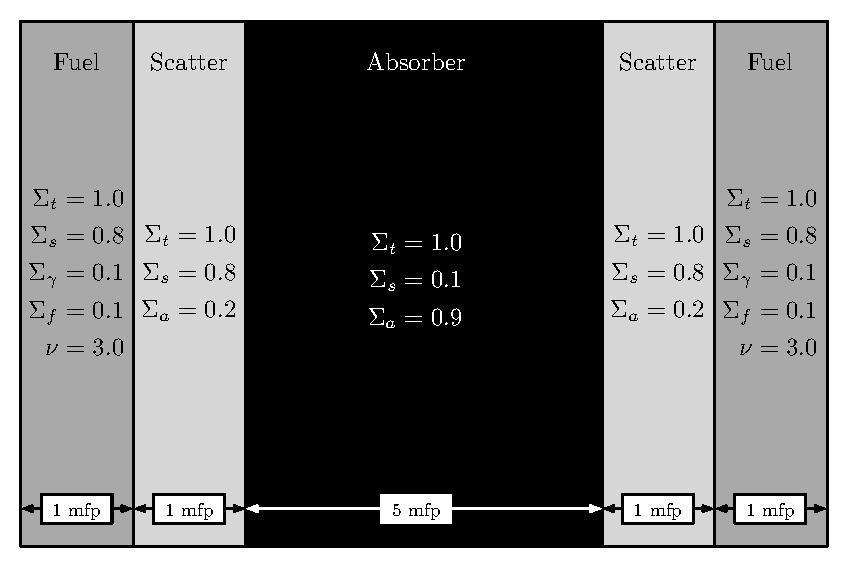
\includegraphics{EntropyandVariance/Data/MultimediaCartoon}
    \caption{Diagram of heterogeneous slab geometry.}
    \label{fig:HeteroGeometry}
\end{figure}

This geometry is particularly difficult for source convergence.  The initial source for this problem lies entirely in the leftmost bin.  With a large highly absorbing slab in the center, it is difficult to move particles from the left to the right side and therefore it will take many histories for the fission source to converge.  The dominance ratio for the symmetric problem is 0.999566 and it is 0.992504 for the asymmetric problem.  For these simulations, 1E5 particles are tracked in each iteration; Arnoldi's method uses 10 iterations per restart and calculated 2 eigenvalues.

The results for the asymmetric problem will be shown first; with a smaller dominance ratio it should be easier to converge the fission source and eigenvalue.  \Fref{fig:AsymmetricPower} shows the convergence of the eigenvalue estimates and fission source as calculated by the power method.  In \Fref{fig:AsymmetricArnoldi} are shown the eigenvalue estimates and fission source convergence for Arnoldi's method.  The solid black line again shows the reference eigenvalue from \citet{Kornreich:2002Semi--0} which is 0.427425.  The dashed line shows the Shannon entropy at the end of the simulation for the power method and the mean of the Shannon entropy for Arnoldi's method.  

The differences in convergence between Arnoldi's method and the power method are easy to see by comparing \Fref{fig:AsymmetricPower} and \Fref{fig:AsymmetricArnoldi}.  We see that Arnoldi's method has converged both the eigenvalue and fission source almost immediately, just like with the homogeneous slab.  The power method however requires 800--900 iterations before the eigenvalue estimates have converged and approximately 1200 iterations before the fission source converges.

\begin{figure}[p]\centering
    \subfloat[Power method.]{\label{fig:AsymmetricPower}\input{EntropyandVariance/Data/AsymmetricPower}}

    \subfloat[Arnoldi's method.]{\label{fig:AsymmetricArnoldi}% GNUPLOT: LaTeX picture with Postscript
\begingroup%
\makeatletter%
\newcommand{\GNUPLOTspecial}{%
  \@sanitize\catcode`\%=14\relax\special}%
\setlength{\unitlength}{0.0500bp}%
\begin{picture}(8640,5760)(0,0)%
  {\GNUPLOTspecial{"
%!PS-Adobe-2.0 EPSF-2.0
%%Title: AsymmetricArnoldi.tex
%%Creator: gnuplot 4.3 patchlevel 0
%%CreationDate: Sat Aug  1 02:43:44 2009
%%DocumentFonts: 
%%BoundingBox: 0 0 432 288
%%EndComments
%%BeginProlog
/gnudict 256 dict def
gnudict begin
%
% The following true/false flags may be edited by hand if desired.
% The unit line width and grayscale image gamma correction may also be changed.
%
/Color true def
/Blacktext true def
/Solid false def
/Dashlength 1 def
/Landscape false def
/Level1 false def
/Rounded false def
/ClipToBoundingBox false def
/TransparentPatterns false def
/gnulinewidth 5.000 def
/userlinewidth gnulinewidth def
/Gamma 1.0 def
%
/vshift -66 def
/dl1 {
  10.0 Dashlength mul mul
  Rounded { currentlinewidth 0.75 mul sub dup 0 le { pop 0.01 } if } if
} def
/dl2 {
  10.0 Dashlength mul mul
  Rounded { currentlinewidth 0.75 mul add } if
} def
/hpt_ 31.5 def
/vpt_ 31.5 def
/hpt hpt_ def
/vpt vpt_ def
Level1 {} {
/SDict 10 dict def
systemdict /pdfmark known not {
  userdict /pdfmark systemdict /cleartomark get put
} if
SDict begin [
  /Title (AsymmetricArnoldi.tex)
  /Subject (gnuplot plot)
  /Creator (gnuplot 4.3 patchlevel 0)
  /Author (Jeremy Conlin)
%  /Producer (gnuplot)
%  /Keywords ()
  /CreationDate (Sat Aug  1 02:43:44 2009)
  /DOCINFO pdfmark
end
} ifelse
/doclip {
  ClipToBoundingBox {
    newpath 0 0 moveto 432 0 lineto 432 288 lineto 0 288 lineto closepath
    clip
  } if
} def
%
% Gnuplot Prolog Version 4.2 (November 2007)
%
/M {moveto} bind def
/L {lineto} bind def
/R {rmoveto} bind def
/V {rlineto} bind def
/N {newpath moveto} bind def
/Z {closepath} bind def
/C {setrgbcolor} bind def
/f {rlineto fill} bind def
/Gshow {show} def   % May be redefined later in the file to support UTF-8
/vpt2 vpt 2 mul def
/hpt2 hpt 2 mul def
/Lshow {currentpoint stroke M 0 vshift R 
	Blacktext {gsave 0 setgray show grestore} {show} ifelse} def
/Rshow {currentpoint stroke M dup stringwidth pop neg vshift R
	Blacktext {gsave 0 setgray show grestore} {show} ifelse} def
/Cshow {currentpoint stroke M dup stringwidth pop -2 div vshift R 
	Blacktext {gsave 0 setgray show grestore} {show} ifelse} def
/UP {dup vpt_ mul /vpt exch def hpt_ mul /hpt exch def
  /hpt2 hpt 2 mul def /vpt2 vpt 2 mul def} def
/DL {Color {setrgbcolor Solid {pop []} if 0 setdash}
 {pop pop pop 0 setgray Solid {pop []} if 0 setdash} ifelse} def
/BL {stroke userlinewidth 2 mul setlinewidth
	Rounded {1 setlinejoin 1 setlinecap} if} def
/AL {stroke userlinewidth 2 div setlinewidth
	Rounded {1 setlinejoin 1 setlinecap} if} def
/UL {dup gnulinewidth mul /userlinewidth exch def
	dup 1 lt {pop 1} if 10 mul /udl exch def} def
/PL {stroke userlinewidth setlinewidth
	Rounded {1 setlinejoin 1 setlinecap} if} def
% Default Line colors
/LCw {1 1 1} def
/LCb {0 0 0} def
/LCa {0 0 0} def
/LC0 {1 0 0} def
/LC1 {0 1 0} def
/LC2 {0 0 1} def
/LC3 {1 0 1} def
/LC4 {0 1 1} def
/LC5 {1 1 0} def
/LC6 {0 0 0} def
/LC7 {1 0.3 0} def
/LC8 {0.5 0.5 0.5} def
% Default Line Types
/LTw {PL [] 1 setgray} def
/LTb {BL [] LCb DL} def
/LTa {AL [1 udl mul 2 udl mul] 0 setdash LCa setrgbcolor} def
/LT0 {PL [] LC0 DL} def
/LT1 {PL [4 dl1 2 dl2] LC1 DL} def
/LT2 {PL [2 dl1 3 dl2] LC2 DL} def
/LT3 {PL [1 dl1 1.5 dl2] LC3 DL} def
/LT4 {PL [6 dl1 2 dl2 1 dl1 2 dl2] LC4 DL} def
/LT5 {PL [3 dl1 3 dl2 1 dl1 3 dl2] LC5 DL} def
/LT6 {PL [2 dl1 2 dl2 2 dl1 6 dl2] LC6 DL} def
/LT7 {PL [1 dl1 2 dl2 6 dl1 2 dl2 1 dl1 2 dl2] LC7 DL} def
/LT8 {PL [2 dl1 2 dl2 2 dl1 2 dl2 2 dl1 2 dl2 2 dl1 4 dl2] LC8 DL} def
/Pnt {stroke [] 0 setdash gsave 1 setlinecap M 0 0 V stroke grestore} def
/Dia {stroke [] 0 setdash 2 copy vpt add M
  hpt neg vpt neg V hpt vpt neg V
  hpt vpt V hpt neg vpt V closepath stroke
  Pnt} def
/Pls {stroke [] 0 setdash vpt sub M 0 vpt2 V
  currentpoint stroke M
  hpt neg vpt neg R hpt2 0 V stroke
 } def
/Box {stroke [] 0 setdash 2 copy exch hpt sub exch vpt add M
  0 vpt2 neg V hpt2 0 V 0 vpt2 V
  hpt2 neg 0 V closepath stroke
  Pnt} def
/Crs {stroke [] 0 setdash exch hpt sub exch vpt add M
  hpt2 vpt2 neg V currentpoint stroke M
  hpt2 neg 0 R hpt2 vpt2 V stroke} def
/TriU {stroke [] 0 setdash 2 copy vpt 1.12 mul add M
  hpt neg vpt -1.62 mul V
  hpt 2 mul 0 V
  hpt neg vpt 1.62 mul V closepath stroke
  Pnt} def
/Star {2 copy Pls Crs} def
/BoxF {stroke [] 0 setdash exch hpt sub exch vpt add M
  0 vpt2 neg V hpt2 0 V 0 vpt2 V
  hpt2 neg 0 V closepath fill} def
/TriUF {stroke [] 0 setdash vpt 1.12 mul add M
  hpt neg vpt -1.62 mul V
  hpt 2 mul 0 V
  hpt neg vpt 1.62 mul V closepath fill} def
/TriD {stroke [] 0 setdash 2 copy vpt 1.12 mul sub M
  hpt neg vpt 1.62 mul V
  hpt 2 mul 0 V
  hpt neg vpt -1.62 mul V closepath stroke
  Pnt} def
/TriDF {stroke [] 0 setdash vpt 1.12 mul sub M
  hpt neg vpt 1.62 mul V
  hpt 2 mul 0 V
  hpt neg vpt -1.62 mul V closepath fill} def
/DiaF {stroke [] 0 setdash vpt add M
  hpt neg vpt neg V hpt vpt neg V
  hpt vpt V hpt neg vpt V closepath fill} def
/Pent {stroke [] 0 setdash 2 copy gsave
  translate 0 hpt M 4 {72 rotate 0 hpt L} repeat
  closepath stroke grestore Pnt} def
/PentF {stroke [] 0 setdash gsave
  translate 0 hpt M 4 {72 rotate 0 hpt L} repeat
  closepath fill grestore} def
/Circle {stroke [] 0 setdash 2 copy
  hpt 0 360 arc stroke Pnt} def
/CircleF {stroke [] 0 setdash hpt 0 360 arc fill} def
/C0 {BL [] 0 setdash 2 copy moveto vpt 90 450 arc} bind def
/C1 {BL [] 0 setdash 2 copy moveto
	2 copy vpt 0 90 arc closepath fill
	vpt 0 360 arc closepath} bind def
/C2 {BL [] 0 setdash 2 copy moveto
	2 copy vpt 90 180 arc closepath fill
	vpt 0 360 arc closepath} bind def
/C3 {BL [] 0 setdash 2 copy moveto
	2 copy vpt 0 180 arc closepath fill
	vpt 0 360 arc closepath} bind def
/C4 {BL [] 0 setdash 2 copy moveto
	2 copy vpt 180 270 arc closepath fill
	vpt 0 360 arc closepath} bind def
/C5 {BL [] 0 setdash 2 copy moveto
	2 copy vpt 0 90 arc
	2 copy moveto
	2 copy vpt 180 270 arc closepath fill
	vpt 0 360 arc} bind def
/C6 {BL [] 0 setdash 2 copy moveto
	2 copy vpt 90 270 arc closepath fill
	vpt 0 360 arc closepath} bind def
/C7 {BL [] 0 setdash 2 copy moveto
	2 copy vpt 0 270 arc closepath fill
	vpt 0 360 arc closepath} bind def
/C8 {BL [] 0 setdash 2 copy moveto
	2 copy vpt 270 360 arc closepath fill
	vpt 0 360 arc closepath} bind def
/C9 {BL [] 0 setdash 2 copy moveto
	2 copy vpt 270 450 arc closepath fill
	vpt 0 360 arc closepath} bind def
/C10 {BL [] 0 setdash 2 copy 2 copy moveto vpt 270 360 arc closepath fill
	2 copy moveto
	2 copy vpt 90 180 arc closepath fill
	vpt 0 360 arc closepath} bind def
/C11 {BL [] 0 setdash 2 copy moveto
	2 copy vpt 0 180 arc closepath fill
	2 copy moveto
	2 copy vpt 270 360 arc closepath fill
	vpt 0 360 arc closepath} bind def
/C12 {BL [] 0 setdash 2 copy moveto
	2 copy vpt 180 360 arc closepath fill
	vpt 0 360 arc closepath} bind def
/C13 {BL [] 0 setdash 2 copy moveto
	2 copy vpt 0 90 arc closepath fill
	2 copy moveto
	2 copy vpt 180 360 arc closepath fill
	vpt 0 360 arc closepath} bind def
/C14 {BL [] 0 setdash 2 copy moveto
	2 copy vpt 90 360 arc closepath fill
	vpt 0 360 arc} bind def
/C15 {BL [] 0 setdash 2 copy vpt 0 360 arc closepath fill
	vpt 0 360 arc closepath} bind def
/Rec {newpath 4 2 roll moveto 1 index 0 rlineto 0 exch rlineto
	neg 0 rlineto closepath} bind def
/Square {dup Rec} bind def
/Bsquare {vpt sub exch vpt sub exch vpt2 Square} bind def
/S0 {BL [] 0 setdash 2 copy moveto 0 vpt rlineto BL Bsquare} bind def
/S1 {BL [] 0 setdash 2 copy vpt Square fill Bsquare} bind def
/S2 {BL [] 0 setdash 2 copy exch vpt sub exch vpt Square fill Bsquare} bind def
/S3 {BL [] 0 setdash 2 copy exch vpt sub exch vpt2 vpt Rec fill Bsquare} bind def
/S4 {BL [] 0 setdash 2 copy exch vpt sub exch vpt sub vpt Square fill Bsquare} bind def
/S5 {BL [] 0 setdash 2 copy 2 copy vpt Square fill
	exch vpt sub exch vpt sub vpt Square fill Bsquare} bind def
/S6 {BL [] 0 setdash 2 copy exch vpt sub exch vpt sub vpt vpt2 Rec fill Bsquare} bind def
/S7 {BL [] 0 setdash 2 copy exch vpt sub exch vpt sub vpt vpt2 Rec fill
	2 copy vpt Square fill Bsquare} bind def
/S8 {BL [] 0 setdash 2 copy vpt sub vpt Square fill Bsquare} bind def
/S9 {BL [] 0 setdash 2 copy vpt sub vpt vpt2 Rec fill Bsquare} bind def
/S10 {BL [] 0 setdash 2 copy vpt sub vpt Square fill 2 copy exch vpt sub exch vpt Square fill
	Bsquare} bind def
/S11 {BL [] 0 setdash 2 copy vpt sub vpt Square fill 2 copy exch vpt sub exch vpt2 vpt Rec fill
	Bsquare} bind def
/S12 {BL [] 0 setdash 2 copy exch vpt sub exch vpt sub vpt2 vpt Rec fill Bsquare} bind def
/S13 {BL [] 0 setdash 2 copy exch vpt sub exch vpt sub vpt2 vpt Rec fill
	2 copy vpt Square fill Bsquare} bind def
/S14 {BL [] 0 setdash 2 copy exch vpt sub exch vpt sub vpt2 vpt Rec fill
	2 copy exch vpt sub exch vpt Square fill Bsquare} bind def
/S15 {BL [] 0 setdash 2 copy Bsquare fill Bsquare} bind def
/D0 {gsave translate 45 rotate 0 0 S0 stroke grestore} bind def
/D1 {gsave translate 45 rotate 0 0 S1 stroke grestore} bind def
/D2 {gsave translate 45 rotate 0 0 S2 stroke grestore} bind def
/D3 {gsave translate 45 rotate 0 0 S3 stroke grestore} bind def
/D4 {gsave translate 45 rotate 0 0 S4 stroke grestore} bind def
/D5 {gsave translate 45 rotate 0 0 S5 stroke grestore} bind def
/D6 {gsave translate 45 rotate 0 0 S6 stroke grestore} bind def
/D7 {gsave translate 45 rotate 0 0 S7 stroke grestore} bind def
/D8 {gsave translate 45 rotate 0 0 S8 stroke grestore} bind def
/D9 {gsave translate 45 rotate 0 0 S9 stroke grestore} bind def
/D10 {gsave translate 45 rotate 0 0 S10 stroke grestore} bind def
/D11 {gsave translate 45 rotate 0 0 S11 stroke grestore} bind def
/D12 {gsave translate 45 rotate 0 0 S12 stroke grestore} bind def
/D13 {gsave translate 45 rotate 0 0 S13 stroke grestore} bind def
/D14 {gsave translate 45 rotate 0 0 S14 stroke grestore} bind def
/D15 {gsave translate 45 rotate 0 0 S15 stroke grestore} bind def
/DiaE {stroke [] 0 setdash vpt add M
  hpt neg vpt neg V hpt vpt neg V
  hpt vpt V hpt neg vpt V closepath stroke} def
/BoxE {stroke [] 0 setdash exch hpt sub exch vpt add M
  0 vpt2 neg V hpt2 0 V 0 vpt2 V
  hpt2 neg 0 V closepath stroke} def
/TriUE {stroke [] 0 setdash vpt 1.12 mul add M
  hpt neg vpt -1.62 mul V
  hpt 2 mul 0 V
  hpt neg vpt 1.62 mul V closepath stroke} def
/TriDE {stroke [] 0 setdash vpt 1.12 mul sub M
  hpt neg vpt 1.62 mul V
  hpt 2 mul 0 V
  hpt neg vpt -1.62 mul V closepath stroke} def
/PentE {stroke [] 0 setdash gsave
  translate 0 hpt M 4 {72 rotate 0 hpt L} repeat
  closepath stroke grestore} def
/CircE {stroke [] 0 setdash 
  hpt 0 360 arc stroke} def
/Opaque {gsave closepath 1 setgray fill grestore 0 setgray closepath} def
/DiaW {stroke [] 0 setdash vpt add M
  hpt neg vpt neg V hpt vpt neg V
  hpt vpt V hpt neg vpt V Opaque stroke} def
/BoxW {stroke [] 0 setdash exch hpt sub exch vpt add M
  0 vpt2 neg V hpt2 0 V 0 vpt2 V
  hpt2 neg 0 V Opaque stroke} def
/TriUW {stroke [] 0 setdash vpt 1.12 mul add M
  hpt neg vpt -1.62 mul V
  hpt 2 mul 0 V
  hpt neg vpt 1.62 mul V Opaque stroke} def
/TriDW {stroke [] 0 setdash vpt 1.12 mul sub M
  hpt neg vpt 1.62 mul V
  hpt 2 mul 0 V
  hpt neg vpt -1.62 mul V Opaque stroke} def
/PentW {stroke [] 0 setdash gsave
  translate 0 hpt M 4 {72 rotate 0 hpt L} repeat
  Opaque stroke grestore} def
/CircW {stroke [] 0 setdash 
  hpt 0 360 arc Opaque stroke} def
/BoxFill {gsave Rec 1 setgray fill grestore} def
/Density {
  /Fillden exch def
  currentrgbcolor
  /ColB exch def /ColG exch def /ColR exch def
  /ColR ColR Fillden mul Fillden sub 1 add def
  /ColG ColG Fillden mul Fillden sub 1 add def
  /ColB ColB Fillden mul Fillden sub 1 add def
  ColR ColG ColB setrgbcolor} def
/BoxColFill {gsave Rec PolyFill} def
/PolyFill {gsave Density fill grestore grestore} def
/h {rlineto rlineto rlineto gsave closepath fill grestore} bind def
%
% PostScript Level 1 Pattern Fill routine for rectangles
% Usage: x y w h s a XX PatternFill
%	x,y = lower left corner of box to be filled
%	w,h = width and height of box
%	  a = angle in degrees between lines and x-axis
%	 XX = 0/1 for no/yes cross-hatch
%
/PatternFill {gsave /PFa [ 9 2 roll ] def
  PFa 0 get PFa 2 get 2 div add PFa 1 get PFa 3 get 2 div add translate
  PFa 2 get -2 div PFa 3 get -2 div PFa 2 get PFa 3 get Rec
  gsave 1 setgray fill grestore clip
  currentlinewidth 0.5 mul setlinewidth
  /PFs PFa 2 get dup mul PFa 3 get dup mul add sqrt def
  0 0 M PFa 5 get rotate PFs -2 div dup translate
  0 1 PFs PFa 4 get div 1 add floor cvi
	{PFa 4 get mul 0 M 0 PFs V} for
  0 PFa 6 get ne {
	0 1 PFs PFa 4 get div 1 add floor cvi
	{PFa 4 get mul 0 2 1 roll M PFs 0 V} for
 } if
  stroke grestore} def
%
/languagelevel where
 {pop languagelevel} {1} ifelse
 2 lt
	{/InterpretLevel1 true def}
	{/InterpretLevel1 Level1 def}
 ifelse
%
% PostScript level 2 pattern fill definitions
%
/Level2PatternFill {
/Tile8x8 {/PaintType 2 /PatternType 1 /TilingType 1 /BBox [0 0 8 8] /XStep 8 /YStep 8}
	bind def
/KeepColor {currentrgbcolor [/Pattern /DeviceRGB] setcolorspace} bind def
<< Tile8x8
 /PaintProc {0.5 setlinewidth pop 0 0 M 8 8 L 0 8 M 8 0 L stroke} 
>> matrix makepattern
/Pat1 exch def
<< Tile8x8
 /PaintProc {0.5 setlinewidth pop 0 0 M 8 8 L 0 8 M 8 0 L stroke
	0 4 M 4 8 L 8 4 L 4 0 L 0 4 L stroke}
>> matrix makepattern
/Pat2 exch def
<< Tile8x8
 /PaintProc {0.5 setlinewidth pop 0 0 M 0 8 L
	8 8 L 8 0 L 0 0 L fill}
>> matrix makepattern
/Pat3 exch def
<< Tile8x8
 /PaintProc {0.5 setlinewidth pop -4 8 M 8 -4 L
	0 12 M 12 0 L stroke}
>> matrix makepattern
/Pat4 exch def
<< Tile8x8
 /PaintProc {0.5 setlinewidth pop -4 0 M 8 12 L
	0 -4 M 12 8 L stroke}
>> matrix makepattern
/Pat5 exch def
<< Tile8x8
 /PaintProc {0.5 setlinewidth pop -2 8 M 4 -4 L
	0 12 M 8 -4 L 4 12 M 10 0 L stroke}
>> matrix makepattern
/Pat6 exch def
<< Tile8x8
 /PaintProc {0.5 setlinewidth pop -2 0 M 4 12 L
	0 -4 M 8 12 L 4 -4 M 10 8 L stroke}
>> matrix makepattern
/Pat7 exch def
<< Tile8x8
 /PaintProc {0.5 setlinewidth pop 8 -2 M -4 4 L
	12 0 M -4 8 L 12 4 M 0 10 L stroke}
>> matrix makepattern
/Pat8 exch def
<< Tile8x8
 /PaintProc {0.5 setlinewidth pop 0 -2 M 12 4 L
	-4 0 M 12 8 L -4 4 M 8 10 L stroke}
>> matrix makepattern
/Pat9 exch def
/Pattern1 {PatternBgnd KeepColor Pat1 setpattern} bind def
/Pattern2 {PatternBgnd KeepColor Pat2 setpattern} bind def
/Pattern3 {PatternBgnd KeepColor Pat3 setpattern} bind def
/Pattern4 {PatternBgnd KeepColor Landscape {Pat5} {Pat4} ifelse setpattern} bind def
/Pattern5 {PatternBgnd KeepColor Landscape {Pat4} {Pat5} ifelse setpattern} bind def
/Pattern6 {PatternBgnd KeepColor Landscape {Pat9} {Pat6} ifelse setpattern} bind def
/Pattern7 {PatternBgnd KeepColor Landscape {Pat8} {Pat7} ifelse setpattern} bind def
} def
%
%
%End of PostScript Level 2 code
%
/PatternBgnd {
  TransparentPatterns {} {gsave 1 setgray fill grestore} ifelse
} def
%
% Substitute for Level 2 pattern fill codes with
% grayscale if Level 2 support is not selected.
%
/Level1PatternFill {
/Pattern1 {0.250 Density} bind def
/Pattern2 {0.500 Density} bind def
/Pattern3 {0.750 Density} bind def
/Pattern4 {0.125 Density} bind def
/Pattern5 {0.375 Density} bind def
/Pattern6 {0.625 Density} bind def
/Pattern7 {0.875 Density} bind def
} def
%
% Now test for support of Level 2 code
%
Level1 {Level1PatternFill} {Level2PatternFill} ifelse
%
/Symbol-Oblique /Symbol findfont [1 0 .167 1 0 0] makefont
dup length dict begin {1 index /FID eq {pop pop} {def} ifelse} forall
currentdict end definefont pop
end
%%EndProlog
gnudict begin
gsave
doclip
0 0 translate
0.050 0.050 scale
0 setgray
newpath
1.000 UL
LTb
1340 640 M
63 0 V
-63 813 R
63 0 V
-63 813 R
63 0 V
-63 814 R
63 0 V
-63 813 R
63 0 V
-63 813 R
63 0 V
-63 813 R
63 0 V
1340 640 M
0 63 V
0 4816 R
0 -63 V
1948 640 M
0 63 V
0 4816 R
0 -63 V
2556 640 M
0 63 V
0 4816 R
0 -63 V
3164 640 M
0 63 V
0 4816 R
0 -63 V
3772 640 M
0 63 V
0 4816 R
0 -63 V
4380 640 M
0 63 V
0 4816 R
0 -63 V
4987 640 M
0 63 V
0 4816 R
0 -63 V
5595 640 M
0 63 V
0 4816 R
0 -63 V
6203 640 M
0 63 V
0 4816 R
0 -63 V
6811 640 M
0 63 V
0 4816 R
0 -63 V
7419 640 M
0 63 V
0 4816 R
0 -63 V
0 -4816 R
-63 0 V
63 542 R
-63 0 V
63 542 R
-63 0 V
63 542 R
-63 0 V
63 542 R
-63 0 V
63 543 R
-63 0 V
63 542 R
-63 0 V
63 542 R
-63 0 V
63 542 R
-63 0 V
63 542 R
-63 0 V
stroke
1340 5519 N
0 -4879 V
6079 0 V
0 4879 V
-6079 0 V
Z stroke
LCb setrgbcolor
LTb
LCb setrgbcolor
LTb
LCb setrgbcolor
LTb
LCb setrgbcolor
LTb
1.000 UP
1.000 UL
LTb
1.000 UL
LTb
5316 703 N
0 600 V
1983 0 V
0 -600 V
-1983 0 V
Z stroke
5316 1303 M
1983 0 V
stroke
LT0
LCb setrgbcolor
LT0
6636 1103 M
543 0 V
1340 5099 M
24 -121 V
25 47 V
24 -69 V
24 119 V
25 -12 V
24 -110 V
24 158 V
25 42 V
24 -131 V
24 191 V
24 -143 V
25 -94 V
24 86 V
24 -48 V
25 100 V
24 -23 V
24 -57 V
25 118 V
24 -9 V
24 -73 V
25 83 V
24 -42 V
24 49 V
25 -23 V
24 -78 V
24 -39 V
25 -99 V
24 74 V
24 1 V
24 57 V
25 -42 V
24 -41 V
24 78 V
25 147 V
24 110 V
24 -134 V
25 -167 V
24 -1 V
24 74 V
25 150 V
24 3 V
24 -211 V
25 97 V
24 8 V
24 -155 V
25 73 V
24 180 V
24 -284 V
24 199 V
25 -26 V
24 -182 V
24 8 V
25 48 V
24 -20 V
24 163 V
25 -114 V
24 95 V
24 4 V
25 -186 V
24 121 V
24 65 V
25 177 V
24 -212 V
24 135 V
25 -152 V
24 -53 V
24 56 V
24 62 V
25 -33 V
24 125 V
24 -202 V
25 95 V
24 19 V
24 -162 V
25 187 V
24 -36 V
24 -16 V
25 -83 V
24 22 V
24 -24 V
25 269 V
24 -326 V
24 147 V
25 38 V
24 -90 V
24 247 V
24 -337 V
25 10 V
24 24 V
24 221 V
25 -248 V
24 52 V
24 -27 V
25 31 V
24 240 V
24 -208 V
25 67 V
24 -21 V
24 102 V
25 10 V
24 -145 V
24 6 V
stroke 3820 5080 M
25 -40 V
24 43 V
24 37 V
24 -221 V
25 296 V
24 -42 V
24 -92 V
25 -51 V
24 -88 V
24 266 V
25 30 V
24 -20 V
24 -95 V
25 -59 V
24 38 V
24 -22 V
25 10 V
24 -94 V
24 -8 V
25 230 V
24 -181 V
24 55 V
25 262 V
24 -309 V
24 93 V
24 -44 V
25 4 V
24 -175 V
24 159 V
25 -245 V
24 341 V
24 -32 V
25 -112 V
24 -44 V
24 269 V
25 -81 V
24 -130 V
24 36 V
25 -87 V
24 116 V
24 -35 V
25 -47 V
24 -33 V
24 116 V
24 3 V
25 -58 V
24 95 V
24 -60 V
25 157 V
24 -130 V
24 -128 V
25 69 V
24 -9 V
24 127 V
25 -106 V
24 6 V
24 -94 V
25 182 V
24 -129 V
24 -96 V
25 179 V
24 17 V
24 -53 V
24 147 V
25 -226 V
24 152 V
24 -133 V
25 -120 V
24 33 V
24 218 V
25 -73 V
24 -110 V
24 -23 V
25 155 V
24 166 V
24 -147 V
25 -146 V
24 237 V
24 -237 V
25 54 V
24 142 V
24 -27 V
24 -88 V
25 12 V
24 130 V
24 -95 V
25 -10 V
24 -265 V
24 247 V
25 107 V
24 -183 V
24 66 V
25 58 V
24 50 V
24 -146 V
25 -141 V
24 163 V
24 2 V
25 39 V
24 134 V
24 -72 V
24 -259 V
25 108 V
24 133 V
stroke 6349 5118 M
24 125 V
25 -319 V
24 96 V
24 45 V
25 -107 V
24 -47 V
24 224 V
25 -38 V
24 -45 V
24 119 V
25 -98 V
24 39 V
24 30 V
25 -158 V
24 -58 V
24 118 V
24 28 V
25 16 V
24 90 V
24 -205 V
25 34 V
24 184 V
24 -33 V
25 -169 V
24 190 V
24 -235 V
25 209 V
24 -13 V
24 -195 V
25 148 V
24 58 V
24 -147 V
25 4 V
24 -16 V
24 101 V
24 48 V
25 -268 V
24 257 V
24 -22 V
25 3 V
24 147 V
24 -183 V
25 -108 V
stroke
2.000 UL
LTb
1340 5100 M
61 0 V
61 0 V
61 0 V
62 0 V
61 0 V
61 0 V
61 0 V
61 0 V
61 0 V
62 0 V
61 0 V
61 0 V
61 0 V
61 0 V
61 0 V
62 0 V
61 0 V
61 0 V
61 0 V
61 0 V
61 0 V
61 0 V
62 0 V
61 0 V
61 0 V
61 0 V
61 0 V
61 0 V
62 0 V
61 0 V
61 0 V
61 0 V
61 0 V
61 0 V
62 0 V
61 0 V
61 0 V
61 0 V
61 0 V
61 0 V
61 0 V
62 0 V
61 0 V
61 0 V
61 0 V
61 0 V
61 0 V
62 0 V
61 0 V
61 0 V
61 0 V
61 0 V
61 0 V
62 0 V
61 0 V
61 0 V
61 0 V
61 0 V
61 0 V
62 0 V
61 0 V
61 0 V
61 0 V
61 0 V
61 0 V
61 0 V
62 0 V
61 0 V
61 0 V
61 0 V
61 0 V
61 0 V
62 0 V
61 0 V
61 0 V
61 0 V
61 0 V
61 0 V
62 0 V
61 0 V
61 0 V
61 0 V
61 0 V
61 0 V
61 0 V
62 0 V
61 0 V
61 0 V
61 0 V
61 0 V
61 0 V
62 0 V
61 0 V
61 0 V
61 0 V
61 0 V
61 0 V
62 0 V
61 0 V
stroke
1.000 UL
LT0
LC2 setrgbcolor
LCb setrgbcolor
LT0
LC2 setrgbcolor
6636 903 M
543 0 V
1343 640 M
21 3019 V
25 286 V
24 -12 V
24 -44 V
25 -255 V
24 -207 V
24 111 V
25 -158 V
24 -192 V
24 593 V
24 -704 V
25 223 V
24 315 V
24 649 V
25 -267 V
24 -64 V
24 -329 V
25 -43 V
24 -12 V
24 206 V
25 -205 V
24 78 V
24 170 V
25 -355 V
24 308 V
24 -48 V
25 -41 V
24 -389 V
24 236 V
24 -175 V
25 306 V
24 -361 V
24 -405 V
25 782 V
24 47 V
24 -24 V
25 146 V
24 -16 V
24 -660 V
25 439 V
24 182 V
24 -148 V
25 -112 V
24 78 V
24 -313 V
25 772 V
24 -1022 V
24 621 V
24 -302 V
25 164 V
24 -313 V
24 698 V
25 -131 V
24 -625 V
24 630 V
25 130 V
24 -376 V
24 84 V
25 120 V
24 -596 V
24 645 V
25 -74 V
24 125 V
24 75 V
25 -382 V
24 -201 V
24 338 V
24 -8 V
25 -208 V
24 367 V
24 454 V
25 -445 V
24 -206 V
24 -596 V
25 314 V
24 402 V
24 107 V
25 156 V
24 -395 V
24 212 V
25 -445 V
24 349 V
24 -473 V
25 -120 V
24 696 V
24 -443 V
24 -630 V
25 623 V
24 -133 V
24 509 V
25 -95 V
24 -308 V
24 365 V
25 113 V
24 -120 V
24 -474 V
25 -562 V
24 687 V
24 243 V
25 -276 V
24 277 V
24 -76 V
stroke 3820 3516 M
25 -333 V
24 131 V
24 513 V
24 9 V
25 -247 V
24 -47 V
24 98 V
25 -444 V
24 642 V
24 138 V
25 -262 V
24 65 V
24 65 V
25 -111 V
24 74 V
24 -132 V
25 -295 V
24 303 V
24 111 V
25 -174 V
24 -456 V
24 493 V
25 -302 V
24 344 V
24 -369 V
24 392 V
25 -228 V
24 -367 V
24 54 V
25 113 V
24 656 V
24 -453 V
25 -110 V
24 471 V
24 -997 V
25 234 V
24 518 V
24 -353 V
25 428 V
24 -125 V
24 -283 V
25 764 V
24 -553 V
24 306 V
24 2 V
25 -655 V
24 99 V
24 411 V
25 -209 V
24 263 V
24 298 V
25 202 V
24 -910 V
24 -539 V
25 971 V
24 93 V
24 -413 V
25 263 V
24 -30 V
24 469 V
25 -522 V
24 -57 V
24 309 V
24 -223 V
25 -502 V
24 370 V
24 -562 V
25 376 V
24 474 V
24 -31 V
25 -161 V
24 -61 V
24 -617 V
25 340 V
24 324 V
24 -307 V
25 -88 V
24 381 V
24 102 V
25 -223 V
24 579 V
24 -268 V
24 -195 V
25 69 V
24 148 V
24 -249 V
25 127 V
24 -599 V
24 148 V
25 207 V
24 77 V
24 36 V
25 -43 V
24 -504 V
24 607 V
25 249 V
24 34 V
24 160 V
25 -498 V
24 -100 V
24 85 V
24 135 V
25 290 V
24 -469 V
stroke 6349 3460 M
24 -50 V
25 81 V
24 -383 V
24 753 V
25 -170 V
24 -179 V
24 259 V
25 -153 V
24 -187 V
24 -232 V
25 67 V
24 87 V
24 319 V
25 99 V
24 -150 V
24 71 V
24 90 V
25 38 V
24 -930 V
24 837 V
25 163 V
24 -925 V
24 969 V
25 -413 V
24 -42 V
24 306 V
25 -416 V
24 157 V
24 116 V
25 149 V
24 -260 V
24 -308 V
25 90 V
24 14 V
24 33 V
24 310 V
25 -47 V
24 -153 V
24 -167 V
25 677 V
24 -254 V
24 64 V
25 -465 V
stroke
2.000 UL
LT1
LCb setrgbcolor
1340 3538 M
61 0 V
61 0 V
61 0 V
62 0 V
61 0 V
61 0 V
61 0 V
61 0 V
61 0 V
62 0 V
61 0 V
61 0 V
61 0 V
61 0 V
61 0 V
62 0 V
61 0 V
61 0 V
61 0 V
61 0 V
61 0 V
61 0 V
62 0 V
61 0 V
61 0 V
61 0 V
61 0 V
61 0 V
62 0 V
61 0 V
61 0 V
61 0 V
61 0 V
61 0 V
62 0 V
61 0 V
61 0 V
61 0 V
61 0 V
61 0 V
61 0 V
62 0 V
61 0 V
61 0 V
61 0 V
61 0 V
61 0 V
62 0 V
61 0 V
61 0 V
61 0 V
61 0 V
61 0 V
62 0 V
61 0 V
61 0 V
61 0 V
61 0 V
61 0 V
62 0 V
61 0 V
61 0 V
61 0 V
61 0 V
61 0 V
61 0 V
62 0 V
61 0 V
61 0 V
61 0 V
61 0 V
61 0 V
62 0 V
61 0 V
61 0 V
61 0 V
61 0 V
61 0 V
62 0 V
61 0 V
61 0 V
61 0 V
61 0 V
61 0 V
61 0 V
62 0 V
61 0 V
61 0 V
61 0 V
61 0 V
61 0 V
62 0 V
61 0 V
61 0 V
61 0 V
61 0 V
61 0 V
62 0 V
61 0 V
stroke
1.000 UL
LTb
1340 5519 N
0 -4879 V
6079 0 V
0 4879 V
-6079 0 V
Z stroke
1.000 UP
1.000 UL
LTb
stroke
grestore
end
showpage
  }}%
  \put(6516,903){\makebox(0,0)[r]{\strut{}Entropy}}%
  \put(6516,1103){\makebox(0,0)[r]{\strut{}Eigenvalue}}%
  \put(4379,140){\makebox(0,0){\strut{}Iteration}}%
  \put(8238,3079){%
  \special{ps: gsave currentpoint currentpoint translate
630 rotate neg exch neg exch translate}%
  \makebox(0,0){\strut{}Shannon Entropy}%
  \special{ps: currentpoint grestore moveto}%
  }%
  \put(280,3079){%
  \special{ps: gsave currentpoint currentpoint translate
630 rotate neg exch neg exch translate}%
  \makebox(0,0){\strut{}Eigenvalue Estimate}%
  \special{ps: currentpoint grestore moveto}%
  }%
  \put(7539,5519){\makebox(0,0)[l]{\strut{} 4.3}}%
  \put(7539,4977){\makebox(0,0)[l]{\strut{} 4.2}}%
  \put(7539,4435){\makebox(0,0)[l]{\strut{} 4.1}}%
  \put(7539,3893){\makebox(0,0)[l]{\strut{} 4}}%
  \put(7539,3351){\makebox(0,0)[l]{\strut{} 3.9}}%
  \put(7539,2808){\makebox(0,0)[l]{\strut{} 3.8}}%
  \put(7539,2266){\makebox(0,0)[l]{\strut{} 3.7}}%
  \put(7539,1724){\makebox(0,0)[l]{\strut{} 3.6}}%
  \put(7539,1182){\makebox(0,0)[l]{\strut{} 3.5}}%
  \put(7539,640){\makebox(0,0)[l]{\strut{} 3.4}}%
  \put(7419,440){\makebox(0,0){\strut{} 2500}}%
  \put(6811,440){\makebox(0,0){\strut{} 2250}}%
  \put(6203,440){\makebox(0,0){\strut{} 2000}}%
  \put(5595,440){\makebox(0,0){\strut{} 1750}}%
  \put(4987,440){\makebox(0,0){\strut{} 1500}}%
  \put(4380,440){\makebox(0,0){\strut{} 1250}}%
  \put(3772,440){\makebox(0,0){\strut{} 1000}}%
  \put(3164,440){\makebox(0,0){\strut{} 750}}%
  \put(2556,440){\makebox(0,0){\strut{} 500}}%
  \put(1948,440){\makebox(0,0){\strut{} 250}}%
  \put(1340,440){\makebox(0,0){\strut{} 0}}%
  \put(1220,5519){\makebox(0,0)[r]{\strut{} 0.43}}%
  \put(1220,4706){\makebox(0,0)[r]{\strut{} 0.425}}%
  \put(1220,3893){\makebox(0,0)[r]{\strut{} 0.42}}%
  \put(1220,3080){\makebox(0,0)[r]{\strut{} 0.415}}%
  \put(1220,2266){\makebox(0,0)[r]{\strut{} 0.41}}%
  \put(1220,1453){\makebox(0,0)[r]{\strut{} 0.405}}%
  \put(1220,640){\makebox(0,0)[r]{\strut{} 0.4}}%
\end{picture}%
\endgroup
\endinput
}
    \caption{Convergence of eigenvalue estimate and Shannon entropy for asymmetric geometry.  Solid black line is the fundamental eigenvalue ($\lambda_0 = 0.427425$ \cite{Kornreich:2002Semi--0}); dashed black line is the entropy at the end of the simulation for the power method and mean entropy for Arnoldi's method.}
\end{figure}

The symmetric problem shows a different convergence for the power method as displayed in \Fref{fig:SymmetricPower}.  \Fref{fig:SymmetricArnoldi} shows convergence of the eigenvalue estimates and fission source as calculated by Arnoldi's method.  The solid black lines show the published eigenvalue \cite{Kornreich:2002Semi--0}, 0.424316.  The dashed black line for the power method shows the final value of the Shannon entropy.  The dashed black line for Arnoldi's method shows the mean value of the Shannon entropy.

In the power method we see that the eigenvalue estimate has converged almost immediately, but the fission source takes much longer to converge.  The power method ran for an extra 2000 iterations and it looks like the fission source might be converged after 4500 iterations, but it looks like the Shannon entropy may still be trending upwards and therefore still has not converged.  In Arnoldi's method both the eigenvalue estimate and the fission source from Arnoldi's method have converged almost immediately.

\begin{figure}[p]\centering
    \subfloat[Power Method]{\label{fig:SymmetricPower}% GNUPLOT: LaTeX picture with Postscript
\begingroup%
\makeatletter%
\newcommand{\GNUPLOTspecial}{%
  \@sanitize\catcode`\%=14\relax\special}%
\setlength{\unitlength}{0.0500bp}%
\begin{picture}(8640,5760)(0,0)%
  {\GNUPLOTspecial{"
%!PS-Adobe-2.0 EPSF-2.0
%%Title: SymmetricPower.tex
%%Creator: gnuplot 4.3 patchlevel 0
%%CreationDate: Sat Aug  1 02:56:23 2009
%%DocumentFonts: 
%%BoundingBox: 0 0 432 288
%%EndComments
%%BeginProlog
/gnudict 256 dict def
gnudict begin
%
% The following true/false flags may be edited by hand if desired.
% The unit line width and grayscale image gamma correction may also be changed.
%
/Color true def
/Blacktext true def
/Solid false def
/Dashlength 1 def
/Landscape false def
/Level1 false def
/Rounded false def
/ClipToBoundingBox false def
/TransparentPatterns false def
/gnulinewidth 5.000 def
/userlinewidth gnulinewidth def
/Gamma 1.0 def
%
/vshift -66 def
/dl1 {
  10.0 Dashlength mul mul
  Rounded { currentlinewidth 0.75 mul sub dup 0 le { pop 0.01 } if } if
} def
/dl2 {
  10.0 Dashlength mul mul
  Rounded { currentlinewidth 0.75 mul add } if
} def
/hpt_ 31.5 def
/vpt_ 31.5 def
/hpt hpt_ def
/vpt vpt_ def
Level1 {} {
/SDict 10 dict def
systemdict /pdfmark known not {
  userdict /pdfmark systemdict /cleartomark get put
} if
SDict begin [
  /Title (SymmetricPower.tex)
  /Subject (gnuplot plot)
  /Creator (gnuplot 4.3 patchlevel 0)
  /Author (Jeremy Conlin)
%  /Producer (gnuplot)
%  /Keywords ()
  /CreationDate (Sat Aug  1 02:56:23 2009)
  /DOCINFO pdfmark
end
} ifelse
/doclip {
  ClipToBoundingBox {
    newpath 0 0 moveto 432 0 lineto 432 288 lineto 0 288 lineto closepath
    clip
  } if
} def
%
% Gnuplot Prolog Version 4.2 (November 2007)
%
/M {moveto} bind def
/L {lineto} bind def
/R {rmoveto} bind def
/V {rlineto} bind def
/N {newpath moveto} bind def
/Z {closepath} bind def
/C {setrgbcolor} bind def
/f {rlineto fill} bind def
/Gshow {show} def   % May be redefined later in the file to support UTF-8
/vpt2 vpt 2 mul def
/hpt2 hpt 2 mul def
/Lshow {currentpoint stroke M 0 vshift R 
	Blacktext {gsave 0 setgray show grestore} {show} ifelse} def
/Rshow {currentpoint stroke M dup stringwidth pop neg vshift R
	Blacktext {gsave 0 setgray show grestore} {show} ifelse} def
/Cshow {currentpoint stroke M dup stringwidth pop -2 div vshift R 
	Blacktext {gsave 0 setgray show grestore} {show} ifelse} def
/UP {dup vpt_ mul /vpt exch def hpt_ mul /hpt exch def
  /hpt2 hpt 2 mul def /vpt2 vpt 2 mul def} def
/DL {Color {setrgbcolor Solid {pop []} if 0 setdash}
 {pop pop pop 0 setgray Solid {pop []} if 0 setdash} ifelse} def
/BL {stroke userlinewidth 2 mul setlinewidth
	Rounded {1 setlinejoin 1 setlinecap} if} def
/AL {stroke userlinewidth 2 div setlinewidth
	Rounded {1 setlinejoin 1 setlinecap} if} def
/UL {dup gnulinewidth mul /userlinewidth exch def
	dup 1 lt {pop 1} if 10 mul /udl exch def} def
/PL {stroke userlinewidth setlinewidth
	Rounded {1 setlinejoin 1 setlinecap} if} def
% Default Line colors
/LCw {1 1 1} def
/LCb {0 0 0} def
/LCa {0 0 0} def
/LC0 {1 0 0} def
/LC1 {0 1 0} def
/LC2 {0 0 1} def
/LC3 {1 0 1} def
/LC4 {0 1 1} def
/LC5 {1 1 0} def
/LC6 {0 0 0} def
/LC7 {1 0.3 0} def
/LC8 {0.5 0.5 0.5} def
% Default Line Types
/LTw {PL [] 1 setgray} def
/LTb {BL [] LCb DL} def
/LTa {AL [1 udl mul 2 udl mul] 0 setdash LCa setrgbcolor} def
/LT0 {PL [] LC0 DL} def
/LT1 {PL [4 dl1 2 dl2] LC1 DL} def
/LT2 {PL [2 dl1 3 dl2] LC2 DL} def
/LT3 {PL [1 dl1 1.5 dl2] LC3 DL} def
/LT4 {PL [6 dl1 2 dl2 1 dl1 2 dl2] LC4 DL} def
/LT5 {PL [3 dl1 3 dl2 1 dl1 3 dl2] LC5 DL} def
/LT6 {PL [2 dl1 2 dl2 2 dl1 6 dl2] LC6 DL} def
/LT7 {PL [1 dl1 2 dl2 6 dl1 2 dl2 1 dl1 2 dl2] LC7 DL} def
/LT8 {PL [2 dl1 2 dl2 2 dl1 2 dl2 2 dl1 2 dl2 2 dl1 4 dl2] LC8 DL} def
/Pnt {stroke [] 0 setdash gsave 1 setlinecap M 0 0 V stroke grestore} def
/Dia {stroke [] 0 setdash 2 copy vpt add M
  hpt neg vpt neg V hpt vpt neg V
  hpt vpt V hpt neg vpt V closepath stroke
  Pnt} def
/Pls {stroke [] 0 setdash vpt sub M 0 vpt2 V
  currentpoint stroke M
  hpt neg vpt neg R hpt2 0 V stroke
 } def
/Box {stroke [] 0 setdash 2 copy exch hpt sub exch vpt add M
  0 vpt2 neg V hpt2 0 V 0 vpt2 V
  hpt2 neg 0 V closepath stroke
  Pnt} def
/Crs {stroke [] 0 setdash exch hpt sub exch vpt add M
  hpt2 vpt2 neg V currentpoint stroke M
  hpt2 neg 0 R hpt2 vpt2 V stroke} def
/TriU {stroke [] 0 setdash 2 copy vpt 1.12 mul add M
  hpt neg vpt -1.62 mul V
  hpt 2 mul 0 V
  hpt neg vpt 1.62 mul V closepath stroke
  Pnt} def
/Star {2 copy Pls Crs} def
/BoxF {stroke [] 0 setdash exch hpt sub exch vpt add M
  0 vpt2 neg V hpt2 0 V 0 vpt2 V
  hpt2 neg 0 V closepath fill} def
/TriUF {stroke [] 0 setdash vpt 1.12 mul add M
  hpt neg vpt -1.62 mul V
  hpt 2 mul 0 V
  hpt neg vpt 1.62 mul V closepath fill} def
/TriD {stroke [] 0 setdash 2 copy vpt 1.12 mul sub M
  hpt neg vpt 1.62 mul V
  hpt 2 mul 0 V
  hpt neg vpt -1.62 mul V closepath stroke
  Pnt} def
/TriDF {stroke [] 0 setdash vpt 1.12 mul sub M
  hpt neg vpt 1.62 mul V
  hpt 2 mul 0 V
  hpt neg vpt -1.62 mul V closepath fill} def
/DiaF {stroke [] 0 setdash vpt add M
  hpt neg vpt neg V hpt vpt neg V
  hpt vpt V hpt neg vpt V closepath fill} def
/Pent {stroke [] 0 setdash 2 copy gsave
  translate 0 hpt M 4 {72 rotate 0 hpt L} repeat
  closepath stroke grestore Pnt} def
/PentF {stroke [] 0 setdash gsave
  translate 0 hpt M 4 {72 rotate 0 hpt L} repeat
  closepath fill grestore} def
/Circle {stroke [] 0 setdash 2 copy
  hpt 0 360 arc stroke Pnt} def
/CircleF {stroke [] 0 setdash hpt 0 360 arc fill} def
/C0 {BL [] 0 setdash 2 copy moveto vpt 90 450 arc} bind def
/C1 {BL [] 0 setdash 2 copy moveto
	2 copy vpt 0 90 arc closepath fill
	vpt 0 360 arc closepath} bind def
/C2 {BL [] 0 setdash 2 copy moveto
	2 copy vpt 90 180 arc closepath fill
	vpt 0 360 arc closepath} bind def
/C3 {BL [] 0 setdash 2 copy moveto
	2 copy vpt 0 180 arc closepath fill
	vpt 0 360 arc closepath} bind def
/C4 {BL [] 0 setdash 2 copy moveto
	2 copy vpt 180 270 arc closepath fill
	vpt 0 360 arc closepath} bind def
/C5 {BL [] 0 setdash 2 copy moveto
	2 copy vpt 0 90 arc
	2 copy moveto
	2 copy vpt 180 270 arc closepath fill
	vpt 0 360 arc} bind def
/C6 {BL [] 0 setdash 2 copy moveto
	2 copy vpt 90 270 arc closepath fill
	vpt 0 360 arc closepath} bind def
/C7 {BL [] 0 setdash 2 copy moveto
	2 copy vpt 0 270 arc closepath fill
	vpt 0 360 arc closepath} bind def
/C8 {BL [] 0 setdash 2 copy moveto
	2 copy vpt 270 360 arc closepath fill
	vpt 0 360 arc closepath} bind def
/C9 {BL [] 0 setdash 2 copy moveto
	2 copy vpt 270 450 arc closepath fill
	vpt 0 360 arc closepath} bind def
/C10 {BL [] 0 setdash 2 copy 2 copy moveto vpt 270 360 arc closepath fill
	2 copy moveto
	2 copy vpt 90 180 arc closepath fill
	vpt 0 360 arc closepath} bind def
/C11 {BL [] 0 setdash 2 copy moveto
	2 copy vpt 0 180 arc closepath fill
	2 copy moveto
	2 copy vpt 270 360 arc closepath fill
	vpt 0 360 arc closepath} bind def
/C12 {BL [] 0 setdash 2 copy moveto
	2 copy vpt 180 360 arc closepath fill
	vpt 0 360 arc closepath} bind def
/C13 {BL [] 0 setdash 2 copy moveto
	2 copy vpt 0 90 arc closepath fill
	2 copy moveto
	2 copy vpt 180 360 arc closepath fill
	vpt 0 360 arc closepath} bind def
/C14 {BL [] 0 setdash 2 copy moveto
	2 copy vpt 90 360 arc closepath fill
	vpt 0 360 arc} bind def
/C15 {BL [] 0 setdash 2 copy vpt 0 360 arc closepath fill
	vpt 0 360 arc closepath} bind def
/Rec {newpath 4 2 roll moveto 1 index 0 rlineto 0 exch rlineto
	neg 0 rlineto closepath} bind def
/Square {dup Rec} bind def
/Bsquare {vpt sub exch vpt sub exch vpt2 Square} bind def
/S0 {BL [] 0 setdash 2 copy moveto 0 vpt rlineto BL Bsquare} bind def
/S1 {BL [] 0 setdash 2 copy vpt Square fill Bsquare} bind def
/S2 {BL [] 0 setdash 2 copy exch vpt sub exch vpt Square fill Bsquare} bind def
/S3 {BL [] 0 setdash 2 copy exch vpt sub exch vpt2 vpt Rec fill Bsquare} bind def
/S4 {BL [] 0 setdash 2 copy exch vpt sub exch vpt sub vpt Square fill Bsquare} bind def
/S5 {BL [] 0 setdash 2 copy 2 copy vpt Square fill
	exch vpt sub exch vpt sub vpt Square fill Bsquare} bind def
/S6 {BL [] 0 setdash 2 copy exch vpt sub exch vpt sub vpt vpt2 Rec fill Bsquare} bind def
/S7 {BL [] 0 setdash 2 copy exch vpt sub exch vpt sub vpt vpt2 Rec fill
	2 copy vpt Square fill Bsquare} bind def
/S8 {BL [] 0 setdash 2 copy vpt sub vpt Square fill Bsquare} bind def
/S9 {BL [] 0 setdash 2 copy vpt sub vpt vpt2 Rec fill Bsquare} bind def
/S10 {BL [] 0 setdash 2 copy vpt sub vpt Square fill 2 copy exch vpt sub exch vpt Square fill
	Bsquare} bind def
/S11 {BL [] 0 setdash 2 copy vpt sub vpt Square fill 2 copy exch vpt sub exch vpt2 vpt Rec fill
	Bsquare} bind def
/S12 {BL [] 0 setdash 2 copy exch vpt sub exch vpt sub vpt2 vpt Rec fill Bsquare} bind def
/S13 {BL [] 0 setdash 2 copy exch vpt sub exch vpt sub vpt2 vpt Rec fill
	2 copy vpt Square fill Bsquare} bind def
/S14 {BL [] 0 setdash 2 copy exch vpt sub exch vpt sub vpt2 vpt Rec fill
	2 copy exch vpt sub exch vpt Square fill Bsquare} bind def
/S15 {BL [] 0 setdash 2 copy Bsquare fill Bsquare} bind def
/D0 {gsave translate 45 rotate 0 0 S0 stroke grestore} bind def
/D1 {gsave translate 45 rotate 0 0 S1 stroke grestore} bind def
/D2 {gsave translate 45 rotate 0 0 S2 stroke grestore} bind def
/D3 {gsave translate 45 rotate 0 0 S3 stroke grestore} bind def
/D4 {gsave translate 45 rotate 0 0 S4 stroke grestore} bind def
/D5 {gsave translate 45 rotate 0 0 S5 stroke grestore} bind def
/D6 {gsave translate 45 rotate 0 0 S6 stroke grestore} bind def
/D7 {gsave translate 45 rotate 0 0 S7 stroke grestore} bind def
/D8 {gsave translate 45 rotate 0 0 S8 stroke grestore} bind def
/D9 {gsave translate 45 rotate 0 0 S9 stroke grestore} bind def
/D10 {gsave translate 45 rotate 0 0 S10 stroke grestore} bind def
/D11 {gsave translate 45 rotate 0 0 S11 stroke grestore} bind def
/D12 {gsave translate 45 rotate 0 0 S12 stroke grestore} bind def
/D13 {gsave translate 45 rotate 0 0 S13 stroke grestore} bind def
/D14 {gsave translate 45 rotate 0 0 S14 stroke grestore} bind def
/D15 {gsave translate 45 rotate 0 0 S15 stroke grestore} bind def
/DiaE {stroke [] 0 setdash vpt add M
  hpt neg vpt neg V hpt vpt neg V
  hpt vpt V hpt neg vpt V closepath stroke} def
/BoxE {stroke [] 0 setdash exch hpt sub exch vpt add M
  0 vpt2 neg V hpt2 0 V 0 vpt2 V
  hpt2 neg 0 V closepath stroke} def
/TriUE {stroke [] 0 setdash vpt 1.12 mul add M
  hpt neg vpt -1.62 mul V
  hpt 2 mul 0 V
  hpt neg vpt 1.62 mul V closepath stroke} def
/TriDE {stroke [] 0 setdash vpt 1.12 mul sub M
  hpt neg vpt 1.62 mul V
  hpt 2 mul 0 V
  hpt neg vpt -1.62 mul V closepath stroke} def
/PentE {stroke [] 0 setdash gsave
  translate 0 hpt M 4 {72 rotate 0 hpt L} repeat
  closepath stroke grestore} def
/CircE {stroke [] 0 setdash 
  hpt 0 360 arc stroke} def
/Opaque {gsave closepath 1 setgray fill grestore 0 setgray closepath} def
/DiaW {stroke [] 0 setdash vpt add M
  hpt neg vpt neg V hpt vpt neg V
  hpt vpt V hpt neg vpt V Opaque stroke} def
/BoxW {stroke [] 0 setdash exch hpt sub exch vpt add M
  0 vpt2 neg V hpt2 0 V 0 vpt2 V
  hpt2 neg 0 V Opaque stroke} def
/TriUW {stroke [] 0 setdash vpt 1.12 mul add M
  hpt neg vpt -1.62 mul V
  hpt 2 mul 0 V
  hpt neg vpt 1.62 mul V Opaque stroke} def
/TriDW {stroke [] 0 setdash vpt 1.12 mul sub M
  hpt neg vpt 1.62 mul V
  hpt 2 mul 0 V
  hpt neg vpt -1.62 mul V Opaque stroke} def
/PentW {stroke [] 0 setdash gsave
  translate 0 hpt M 4 {72 rotate 0 hpt L} repeat
  Opaque stroke grestore} def
/CircW {stroke [] 0 setdash 
  hpt 0 360 arc Opaque stroke} def
/BoxFill {gsave Rec 1 setgray fill grestore} def
/Density {
  /Fillden exch def
  currentrgbcolor
  /ColB exch def /ColG exch def /ColR exch def
  /ColR ColR Fillden mul Fillden sub 1 add def
  /ColG ColG Fillden mul Fillden sub 1 add def
  /ColB ColB Fillden mul Fillden sub 1 add def
  ColR ColG ColB setrgbcolor} def
/BoxColFill {gsave Rec PolyFill} def
/PolyFill {gsave Density fill grestore grestore} def
/h {rlineto rlineto rlineto gsave closepath fill grestore} bind def
%
% PostScript Level 1 Pattern Fill routine for rectangles
% Usage: x y w h s a XX PatternFill
%	x,y = lower left corner of box to be filled
%	w,h = width and height of box
%	  a = angle in degrees between lines and x-axis
%	 XX = 0/1 for no/yes cross-hatch
%
/PatternFill {gsave /PFa [ 9 2 roll ] def
  PFa 0 get PFa 2 get 2 div add PFa 1 get PFa 3 get 2 div add translate
  PFa 2 get -2 div PFa 3 get -2 div PFa 2 get PFa 3 get Rec
  gsave 1 setgray fill grestore clip
  currentlinewidth 0.5 mul setlinewidth
  /PFs PFa 2 get dup mul PFa 3 get dup mul add sqrt def
  0 0 M PFa 5 get rotate PFs -2 div dup translate
  0 1 PFs PFa 4 get div 1 add floor cvi
	{PFa 4 get mul 0 M 0 PFs V} for
  0 PFa 6 get ne {
	0 1 PFs PFa 4 get div 1 add floor cvi
	{PFa 4 get mul 0 2 1 roll M PFs 0 V} for
 } if
  stroke grestore} def
%
/languagelevel where
 {pop languagelevel} {1} ifelse
 2 lt
	{/InterpretLevel1 true def}
	{/InterpretLevel1 Level1 def}
 ifelse
%
% PostScript level 2 pattern fill definitions
%
/Level2PatternFill {
/Tile8x8 {/PaintType 2 /PatternType 1 /TilingType 1 /BBox [0 0 8 8] /XStep 8 /YStep 8}
	bind def
/KeepColor {currentrgbcolor [/Pattern /DeviceRGB] setcolorspace} bind def
<< Tile8x8
 /PaintProc {0.5 setlinewidth pop 0 0 M 8 8 L 0 8 M 8 0 L stroke} 
>> matrix makepattern
/Pat1 exch def
<< Tile8x8
 /PaintProc {0.5 setlinewidth pop 0 0 M 8 8 L 0 8 M 8 0 L stroke
	0 4 M 4 8 L 8 4 L 4 0 L 0 4 L stroke}
>> matrix makepattern
/Pat2 exch def
<< Tile8x8
 /PaintProc {0.5 setlinewidth pop 0 0 M 0 8 L
	8 8 L 8 0 L 0 0 L fill}
>> matrix makepattern
/Pat3 exch def
<< Tile8x8
 /PaintProc {0.5 setlinewidth pop -4 8 M 8 -4 L
	0 12 M 12 0 L stroke}
>> matrix makepattern
/Pat4 exch def
<< Tile8x8
 /PaintProc {0.5 setlinewidth pop -4 0 M 8 12 L
	0 -4 M 12 8 L stroke}
>> matrix makepattern
/Pat5 exch def
<< Tile8x8
 /PaintProc {0.5 setlinewidth pop -2 8 M 4 -4 L
	0 12 M 8 -4 L 4 12 M 10 0 L stroke}
>> matrix makepattern
/Pat6 exch def
<< Tile8x8
 /PaintProc {0.5 setlinewidth pop -2 0 M 4 12 L
	0 -4 M 8 12 L 4 -4 M 10 8 L stroke}
>> matrix makepattern
/Pat7 exch def
<< Tile8x8
 /PaintProc {0.5 setlinewidth pop 8 -2 M -4 4 L
	12 0 M -4 8 L 12 4 M 0 10 L stroke}
>> matrix makepattern
/Pat8 exch def
<< Tile8x8
 /PaintProc {0.5 setlinewidth pop 0 -2 M 12 4 L
	-4 0 M 12 8 L -4 4 M 8 10 L stroke}
>> matrix makepattern
/Pat9 exch def
/Pattern1 {PatternBgnd KeepColor Pat1 setpattern} bind def
/Pattern2 {PatternBgnd KeepColor Pat2 setpattern} bind def
/Pattern3 {PatternBgnd KeepColor Pat3 setpattern} bind def
/Pattern4 {PatternBgnd KeepColor Landscape {Pat5} {Pat4} ifelse setpattern} bind def
/Pattern5 {PatternBgnd KeepColor Landscape {Pat4} {Pat5} ifelse setpattern} bind def
/Pattern6 {PatternBgnd KeepColor Landscape {Pat9} {Pat6} ifelse setpattern} bind def
/Pattern7 {PatternBgnd KeepColor Landscape {Pat8} {Pat7} ifelse setpattern} bind def
} def
%
%
%End of PostScript Level 2 code
%
/PatternBgnd {
  TransparentPatterns {} {gsave 1 setgray fill grestore} ifelse
} def
%
% Substitute for Level 2 pattern fill codes with
% grayscale if Level 2 support is not selected.
%
/Level1PatternFill {
/Pattern1 {0.250 Density} bind def
/Pattern2 {0.500 Density} bind def
/Pattern3 {0.750 Density} bind def
/Pattern4 {0.125 Density} bind def
/Pattern5 {0.375 Density} bind def
/Pattern6 {0.625 Density} bind def
/Pattern7 {0.875 Density} bind def
} def
%
% Now test for support of Level 2 code
%
Level1 {Level1PatternFill} {Level2PatternFill} ifelse
%
/Symbol-Oblique /Symbol findfont [1 0 .167 1 0 0] makefont
dup length dict begin {1 index /FID eq {pop pop} {def} ifelse} forall
currentdict end definefont pop
end
%%EndProlog
gnudict begin
gsave
doclip
0 0 translate
0.050 0.050 scale
0 setgray
newpath
1.000 UL
LTb
1340 640 M
63 0 V
-63 813 R
63 0 V
-63 813 R
63 0 V
-63 814 R
63 0 V
-63 813 R
63 0 V
-63 813 R
63 0 V
-63 813 R
63 0 V
1340 640 M
0 63 V
0 4816 R
0 -63 V
2015 640 M
0 63 V
0 4816 R
0 -63 V
2691 640 M
0 63 V
0 4816 R
0 -63 V
3366 640 M
0 63 V
0 4816 R
0 -63 V
4042 640 M
0 63 V
0 4816 R
0 -63 V
4717 640 M
0 63 V
0 4816 R
0 -63 V
5393 640 M
0 63 V
0 4816 R
0 -63 V
6068 640 M
0 63 V
0 4816 R
0 -63 V
6744 640 M
0 63 V
0 4816 R
0 -63 V
7419 640 M
0 63 V
0 4816 R
0 -63 V
0 -4816 R
-63 0 V
63 574 R
-63 0 V
63 574 R
-63 0 V
63 574 R
-63 0 V
63 574 R
-63 0 V
63 574 R
-63 0 V
63 574 R
-63 0 V
63 574 R
-63 0 V
63 574 R
-63 0 V
stroke
1340 5519 N
0 -4879 V
6079 0 V
0 4879 V
-6079 0 V
Z stroke
LCb setrgbcolor
LTb
LCb setrgbcolor
LTb
LCb setrgbcolor
LTb
LCb setrgbcolor
LTb
1.000 UP
1.000 UL
LTb
1.000 UL
LTb
5316 703 N
0 600 V
1983 0 V
0 -600 V
-1983 0 V
Z stroke
5316 1303 M
1983 0 V
stroke
LT0
LCb setrgbcolor
LT0
6636 1103 M
543 0 V
1341 640 M
0 13 V
2 3207 V
1 560 V
1 175 V
2 -23 V
1 -128 V
1 112 V
2 -126 V
1 265 V
2 -223 V
1 81 V
1 -16 V
2 41 V
1 -143 V
1 178 V
2 101 V
1 -137 V
1 10 V
2 -13 V
1 -72 V
1 168 V
2 -25 V
1 69 V
1 56 V
2 -69 V
1 -119 V
1 -58 V
2 45 V
1 12 V
2 -232 V
1 211 V
1 38 V
2 41 V
1 -111 V
1 109 V
2 70 V
1 -153 V
1 61 V
2 56 V
1 -168 V
1 41 V
2 37 V
1 128 V
1 -76 V
2 -21 V
1 27 V
1 -40 V
2 85 V
1 -25 V
2 -126 V
1 85 V
1 -9 V
2 152 V
1 -172 V
1 -131 V
2 138 V
1 107 V
1 -136 V
2 -2 V
1 58 V
1 -43 V
2 -50 V
1 -151 V
1 197 V
2 73 V
1 -89 V
2 -16 V
1 -3 V
1 -190 V
2 185 V
1 215 V
1 -163 V
2 49 V
1 101 V
1 -141 V
2 137 V
1 -114 V
1 0 V
2 -133 V
1 163 V
1 -171 V
2 275 V
1 -117 V
1 -185 V
2 -15 V
1 134 V
2 62 V
1 -107 V
1 -19 V
2 70 V
1 38 V
1 -118 V
2 251 V
1 -278 V
1 43 V
2 181 V
1 -107 V
1 -105 V
2 -34 V
1 243 V
1 99 V
2 -233 V
stroke 1478 4557 M
1 118 V
1 -13 V
2 -78 V
1 -116 V
2 -9 V
1 191 V
1 -48 V
2 -77 V
1 92 V
1 -3 V
2 -75 V
1 -50 V
1 202 V
2 -61 V
1 -135 V
1 106 V
2 90 V
1 -1 V
1 -134 V
2 12 V
1 -47 V
2 152 V
1 -134 V
1 -49 V
2 202 V
1 -208 V
1 113 V
2 -1 V
1 -73 V
1 -56 V
2 189 V
1 -256 V
1 156 V
2 20 V
1 18 V
1 60 V
2 -150 V
1 125 V
1 -123 V
2 86 V
1 -22 V
2 79 V
1 -93 V
1 -51 V
2 159 V
1 -288 V
1 109 V
2 218 V
1 -4 V
1 -101 V
2 62 V
1 -93 V
1 -94 V
2 128 V
1 150 V
1 -186 V
2 121 V
1 -208 V
1 -30 V
2 270 V
1 -163 V
2 35 V
1 -87 V
1 -4 V
2 51 V
1 163 V
1 -221 V
2 49 V
1 30 V
1 -13 V
2 -31 V
1 85 V
1 -42 V
2 -94 V
1 218 V
1 -133 V
2 -112 V
1 31 V
2 185 V
1 -54 V
1 -118 V
2 102 V
1 -43 V
1 -49 V
2 152 V
1 122 V
1 -208 V
2 -16 V
1 51 V
1 -5 V
2 58 V
1 77 V
1 -277 V
2 128 V
1 70 V
1 -71 V
2 117 V
1 -73 V
2 -66 V
1 -77 V
1 -52 V
2 142 V
1 -130 V
1 189 V
stroke 1618 4634 M
2 122 V
1 -100 V
1 -219 V
2 215 V
1 5 V
1 -90 V
2 17 V
1 23 V
1 -77 V
2 98 V
1 -17 V
1 1 V
2 -7 V
1 -105 V
2 109 V
1 33 V
1 -8 V
2 32 V
1 -74 V
1 -177 V
2 113 V
1 52 V
1 -212 V
2 -9 V
1 218 V
1 -49 V
2 49 V
1 0 V
1 37 V
2 -36 V
1 7 V
2 2 V
1 18 V
1 5 V
2 49 V
1 -20 V
1 76 V
2 -133 V
1 103 V
1 -56 V
2 -119 V
1 88 V
1 -8 V
2 -24 V
1 170 V
1 -49 V
2 -144 V
1 87 V
1 -23 V
2 -106 V
1 132 V
2 96 V
1 -358 V
1 382 V
2 -107 V
1 -110 V
1 67 V
2 -12 V
1 -25 V
1 -83 V
2 98 V
1 -5 V
1 -57 V
2 126 V
1 -62 V
1 -72 V
2 109 V
1 -120 V
1 67 V
2 -35 V
1 68 V
2 -72 V
1 -16 V
1 -21 V
2 51 V
1 99 V
1 -38 V
2 -32 V
1 81 V
1 30 V
2 -76 V
1 -21 V
1 1 V
2 61 V
1 -139 V
1 139 V
2 -190 V
1 321 V
2 -256 V
1 21 V
1 -28 V
2 43 V
1 42 V
1 152 V
2 -108 V
1 -115 V
1 24 V
2 -15 V
1 215 V
1 127 V
2 -235 V
1 -89 V
1 -110 V
2 101 V
stroke 1759 4547 M
1 190 V
1 -6 V
2 -214 V
1 103 V
2 151 V
1 -213 V
1 -102 V
2 92 V
1 193 V
1 -226 V
2 137 V
1 -226 V
1 52 V
2 90 V
1 57 V
1 88 V
2 -33 V
1 -64 V
1 47 V
2 -218 V
1 147 V
1 -42 V
2 56 V
1 -245 V
2 382 V
1 -172 V
1 70 V
2 -128 V
1 181 V
1 -189 V
2 124 V
1 49 V
1 -111 V
2 -29 V
1 -3 V
1 29 V
2 101 V
1 -22 V
1 83 V
2 -108 V
1 -60 V
2 31 V
1 -22 V
1 -92 V
2 16 V
1 26 V
1 232 V
2 -174 V
1 89 V
1 -43 V
2 -125 V
1 -35 V
1 131 V
2 67 V
1 -52 V
1 -2 V
2 18 V
1 -37 V
1 144 V
2 89 V
1 -139 V
2 -211 V
1 70 V
1 -28 V
2 -24 V
1 -87 V
1 153 V
2 -90 V
1 150 V
1 -138 V
2 169 V
1 48 V
1 -104 V
2 1 V
1 12 V
1 -85 V
2 73 V
1 -124 V
1 -65 V
2 271 V
1 -47 V
2 79 V
1 13 V
1 -62 V
2 8 V
1 61 V
1 -159 V
2 -3 V
1 229 V
1 -218 V
2 132 V
1 -63 V
1 -68 V
2 210 V
1 -136 V
1 -205 V
2 63 V
1 120 V
2 -117 V
1 101 V
1 -180 V
2 107 V
1 -34 V
1 41 V
stroke 1899 4543 M
2 12 V
1 148 V
1 -157 V
2 2 V
1 84 V
1 -67 V
2 23 V
1 -40 V
1 144 V
2 -124 V
1 -22 V
1 112 V
2 27 V
1 -240 V
2 185 V
1 20 V
1 -138 V
2 88 V
1 -22 V
1 -62 V
2 121 V
1 -71 V
1 -63 V
2 112 V
1 -20 V
1 -53 V
2 79 V
1 78 V
1 -124 V
2 145 V
1 -9 V
1 -144 V
2 118 V
1 -269 V
2 227 V
1 5 V
1 39 V
2 -183 V
1 125 V
1 -5 V
2 -101 V
1 74 V
1 113 V
2 -158 V
1 134 V
1 -257 V
2 167 V
1 80 V
1 -11 V
2 48 V
1 2 V
2 36 V
1 -217 V
1 154 V
2 -44 V
1 -125 V
1 129 V
2 -100 V
1 -21 V
1 38 V
2 67 V
1 56 V
1 -43 V
2 -137 V
1 157 V
1 -155 V
2 245 V
1 -104 V
1 117 V
2 -109 V
1 -154 V
2 28 V
1 125 V
1 100 V
2 -240 V
1 -6 V
1 46 V
2 55 V
1 -51 V
1 60 V
2 74 V
1 -118 V
1 26 V
2 123 V
1 58 V
1 -342 V
2 150 V
1 32 V
1 -31 V
2 -61 V
1 111 V
2 -70 V
1 20 V
1 -71 V
2 131 V
1 -116 V
1 133 V
2 -35 V
1 -47 V
1 -147 V
2 158 V
1 -79 V
1 45 V
2 -39 V
stroke 2040 4527 M
1 -25 V
1 231 V
2 -349 V
1 254 V
2 -40 V
1 120 V
1 -197 V
2 -49 V
1 164 V
1 6 V
2 -84 V
1 16 V
1 172 V
2 -117 V
1 -140 V
1 88 V
2 -41 V
1 137 V
1 -124 V
2 66 V
1 33 V
1 -121 V
2 60 V
1 -74 V
2 97 V
1 -51 V
1 -36 V
2 250 V
1 -322 V
1 170 V
2 -112 V
1 -20 V
1 42 V
2 34 V
1 53 V
1 -91 V
2 71 V
1 -49 V
1 86 V
2 -130 V
1 141 V
1 -102 V
2 21 V
1 -102 V
2 24 V
1 -37 V
1 162 V
2 52 V
1 68 V
1 11 V
2 -162 V
1 112 V
1 66 V
2 -18 V
1 -131 V
1 -79 V
2 138 V
1 -111 V
1 42 V
2 -97 V
1 174 V
2 -65 V
1 67 V
1 42 V
2 89 V
1 -189 V
1 4 V
2 27 V
1 -221 V
1 240 V
2 -162 V
1 111 V
1 -18 V
2 -78 V
1 34 V
1 153 V
2 -36 V
1 -59 V
1 -179 V
2 178 V
1 -18 V
2 91 V
1 -116 V
1 177 V
2 -204 V
1 149 V
1 -106 V
2 -65 V
1 100 V
1 -23 V
2 -74 V
1 113 V
1 -20 V
2 71 V
1 -216 V
1 -3 V
2 -28 V
1 264 V
1 -199 V
2 141 V
1 49 V
2 -225 V
1 326 V
1 -225 V
stroke 2180 4574 M
2 37 V
1 -26 V
1 -53 V
2 -119 V
1 224 V
1 57 V
2 -5 V
1 -95 V
1 -117 V
2 185 V
1 64 V
1 -68 V
2 -16 V
1 -72 V
2 165 V
1 -298 V
1 194 V
2 -174 V
1 109 V
1 6 V
2 -58 V
1 82 V
1 31 V
2 -7 V
1 71 V
1 -185 V
2 69 V
1 160 V
1 -65 V
2 -124 V
1 56 V
1 -31 V
2 -4 V
1 -11 V
2 4 V
1 -238 V
1 145 V
2 299 V
1 -112 V
1 -88 V
2 -78 V
1 157 V
1 88 V
2 -132 V
1 82 V
1 -166 V
2 86 V
1 -51 V
1 2 V
2 -68 V
1 89 V
1 69 V
2 -6 V
1 78 V
2 -72 V
1 62 V
1 -175 V
2 163 V
1 49 V
1 -314 V
2 154 V
1 107 V
1 -113 V
2 38 V
1 120 V
1 -225 V
2 192 V
1 56 V
1 -105 V
2 -111 V
1 23 V
2 -27 V
1 154 V
1 45 V
2 -131 V
1 -99 V
1 26 V
2 105 V
1 -122 V
1 73 V
2 -8 V
1 -137 V
1 219 V
2 -69 V
1 63 V
1 -70 V
2 85 V
1 -93 V
1 -195 V
2 42 V
1 6 V
2 151 V
1 31 V
1 -127 V
2 144 V
1 -42 V
1 -31 V
2 -13 V
1 137 V
1 87 V
2 -68 V
1 -193 V
1 57 V
2 -23 V
stroke 2321 4542 M
1 40 V
1 192 V
2 -180 V
1 -21 V
1 112 V
2 -24 V
1 -22 V
2 -28 V
1 -86 V
1 140 V
2 -222 V
1 205 V
1 -61 V
2 -63 V
1 52 V
1 129 V
2 -233 V
1 275 V
1 -325 V
2 175 V
1 -92 V
1 104 V
2 106 V
1 -57 V
2 -229 V
1 145 V
1 85 V
2 -63 V
1 -125 V
1 56 V
2 90 V
1 -149 V
1 201 V
2 -61 V
1 -134 V
1 271 V
2 15 V
1 -59 V
1 -132 V
2 -47 V
1 -4 V
1 187 V
2 -76 V
1 -7 V
2 123 V
1 -139 V
1 -91 V
2 19 V
1 261 V
1 -363 V
2 115 V
1 5 V
1 126 V
2 59 V
1 -136 V
1 -93 V
2 81 V
1 -12 V
1 99 V
2 -177 V
1 134 V
2 97 V
1 -30 V
1 -109 V
2 14 V
1 -299 V
1 257 V
2 -59 V
1 89 V
1 86 V
2 -108 V
1 55 V
1 -3 V
2 41 V
1 -285 V
1 158 V
2 -104 V
1 150 V
1 157 V
2 -56 V
1 -115 V
2 -40 V
1 31 V
1 72 V
2 -130 V
1 105 V
1 -187 V
2 207 V
1 -54 V
1 -32 V
2 26 V
1 -51 V
1 -125 V
2 138 V
1 103 V
1 -56 V
2 -44 V
1 138 V
1 -107 V
2 85 V
1 -1 V
2 -149 V
1 259 V
1 -142 V
stroke 2461 4615 M
2 -56 V
1 28 V
1 -188 V
2 97 V
1 108 V
1 -33 V
2 37 V
1 186 V
1 -174 V
2 154 V
1 -174 V
1 -38 V
2 -70 V
1 4 V
2 24 V
1 -86 V
1 137 V
2 -34 V
1 4 V
1 131 V
2 48 V
1 -281 V
1 176 V
2 -48 V
1 217 V
1 -213 V
2 68 V
1 26 V
1 -253 V
2 114 V
1 73 V
1 197 V
2 -256 V
1 87 V
2 102 V
1 22 V
1 -294 V
2 197 V
1 -69 V
1 77 V
2 -74 V
1 -57 V
1 23 V
2 -82 V
1 140 V
1 -18 V
2 -9 V
1 64 V
1 -101 V
2 -20 V
1 -53 V
1 263 V
2 -81 V
1 -95 V
2 88 V
1 49 V
1 -66 V
2 107 V
1 -345 V
1 226 V
2 147 V
1 -84 V
1 -141 V
2 -92 V
1 194 V
1 -174 V
2 125 V
1 2 V
1 20 V
2 153 V
1 -147 V
2 -101 V
1 2 V
1 50 V
2 -96 V
1 219 V
1 73 V
2 -226 V
1 165 V
1 -306 V
2 242 V
1 -41 V
1 -17 V
2 -122 V
1 191 V
1 26 V
2 -199 V
1 188 V
1 -28 V
2 -157 V
1 187 V
2 -203 V
1 178 V
1 16 V
2 -77 V
1 -144 V
1 198 V
2 -67 V
1 163 V
1 -74 V
2 -27 V
1 -108 V
1 47 V
2 79 V
stroke 2602 4655 M
1 -58 V
1 -37 V
2 63 V
1 17 V
1 -42 V
2 -78 V
1 183 V
2 -75 V
1 170 V
1 -129 V
2 40 V
1 -127 V
1 -127 V
2 106 V
1 147 V
1 33 V
2 -126 V
1 -31 V
1 -134 V
2 261 V
1 -187 V
1 -6 V
2 36 V
1 -106 V
2 211 V
1 -42 V
1 -35 V
2 -38 V
1 57 V
1 137 V
2 -146 V
1 70 V
1 -103 V
2 88 V
1 160 V
1 -191 V
2 125 V
1 -85 V
1 -21 V
2 -193 V
1 220 V
1 -98 V
2 35 V
1 61 V
2 -77 V
1 62 V
1 -76 V
2 -161 V
1 224 V
1 5 V
2 -216 V
1 313 V
1 -294 V
2 167 V
1 -49 V
1 -105 V
2 6 V
1 212 V
1 -102 V
2 -13 V
1 86 V
1 -38 V
2 52 V
1 -215 V
2 95 V
1 -4 V
1 144 V
2 -11 V
1 -158 V
1 118 V
2 -103 V
1 85 V
1 -123 V
2 -29 V
1 67 V
1 -7 V
2 142 V
1 -109 V
1 -45 V
2 26 V
1 115 V
2 -41 V
1 -187 V
1 205 V
2 -15 V
1 -197 V
1 113 V
2 43 V
1 80 V
1 -226 V
2 150 V
1 96 V
1 -7 V
2 -90 V
1 110 V
1 118 V
2 -154 V
1 -36 V
1 90 V
2 -143 V
1 20 V
2 146 V
1 -88 V
1 -128 V
stroke 2742 4503 M
2 228 V
1 -2 V
1 -226 V
2 129 V
1 50 V
1 -111 V
2 -80 V
1 205 V
1 -1 V
2 -336 V
1 213 V
1 71 V
2 -116 V
1 146 V
1 84 V
2 -257 V
1 44 V
2 52 V
1 2 V
1 256 V
2 -244 V
1 10 V
1 -119 V
2 259 V
1 -177 V
1 -72 V
2 -13 V
1 159 V
1 -141 V
2 115 V
1 -20 V
1 -46 V
2 114 V
1 -174 V
2 -5 V
1 114 V
1 -67 V
2 -106 V
1 137 V
1 126 V
2 -86 V
1 -67 V
1 114 V
2 -142 V
1 48 V
1 93 V
2 -1 V
1 -247 V
1 259 V
2 -108 V
1 101 V
1 -69 V
2 3 V
1 -33 V
2 -35 V
1 -71 V
1 110 V
2 -184 V
1 253 V
1 -91 V
2 16 V
1 208 V
1 -235 V
2 179 V
1 -201 V
1 104 V
2 -69 V
1 -18 V
1 78 V
2 4 V
1 98 V
1 -189 V
2 16 V
1 -3 V
2 -76 V
1 188 V
1 91 V
2 -121 V
1 3 V
1 -56 V
2 -55 V
1 223 V
1 -128 V
2 76 V
1 -37 V
1 -87 V
2 122 V
1 -50 V
1 -47 V
2 51 V
1 -94 V
2 99 V
1 -69 V
1 -63 V
2 236 V
1 -153 V
1 -40 V
2 77 V
1 185 V
1 -164 V
2 -40 V
1 169 V
1 -89 V
2 114 V
stroke 2883 4804 M
1 -175 V
1 -37 V
2 96 V
1 -77 V
1 -46 V
2 194 V
1 -4 V
2 -180 V
1 13 V
1 3 V
2 135 V
1 -10 V
1 17 V
2 -154 V
1 119 V
1 -61 V
2 -114 V
1 15 V
1 28 V
2 -116 V
1 296 V
1 -198 V
2 -77 V
1 -25 V
1 122 V
2 31 V
1 27 V
2 109 V
1 -139 V
1 -52 V
2 236 V
1 -137 V
1 -168 V
2 174 V
1 -90 V
1 74 V
2 -52 V
1 73 V
1 -104 V
2 42 V
1 223 V
1 -343 V
2 207 V
1 -179 V
2 -161 V
1 357 V
1 -113 V
2 80 V
1 8 V
1 -7 V
2 -125 V
1 47 V
1 150 V
2 -234 V
1 97 V
1 -52 V
2 75 V
1 -109 V
1 106 V
2 156 V
1 -239 V
1 151 V
2 -3 V
1 -90 V
2 28 V
1 -130 V
1 152 V
2 -56 V
1 -99 V
1 92 V
2 111 V
1 -110 V
1 40 V
2 -84 V
1 6 V
1 56 V
2 -147 V
1 -38 V
1 32 V
2 85 V
1 100 V
1 25 V
2 55 V
1 -52 V
2 -34 V
1 -148 V
1 140 V
2 154 V
1 -168 V
1 40 V
2 -35 V
1 -112 V
1 66 V
2 100 V
1 -11 V
1 11 V
2 -42 V
1 133 V
1 -151 V
2 72 V
1 -20 V
2 -71 V
1 -14 V
1 90 V
stroke 3023 4660 M
2 28 V
1 -247 V
1 170 V
2 -105 V
1 -1 V
1 125 V
2 -27 V
1 153 V
1 -58 V
2 -206 V
1 43 V
1 223 V
2 -204 V
1 27 V
1 -143 V
2 332 V
1 -187 V
2 -64 V
1 40 V
1 -56 V
2 40 V
1 143 V
1 -124 V
2 26 V
1 -66 V
1 109 V
2 52 V
1 -187 V
1 371 V
2 -244 V
1 -27 V
1 -52 V
2 22 V
1 -46 V
1 135 V
2 243 V
1 -298 V
2 26 V
1 -74 V
1 19 V
2 158 V
1 -143 V
1 36 V
2 10 V
1 93 V
1 -220 V
2 87 V
1 -71 V
1 50 V
2 18 V
1 121 V
1 -51 V
2 -31 V
1 -135 V
2 -59 V
1 58 V
1 218 V
2 -111 V
1 119 V
1 -91 V
2 18 V
1 66 V
1 -143 V
2 188 V
1 -149 V
1 -71 V
2 76 V
1 33 V
1 -166 V
2 138 V
1 108 V
1 -190 V
2 105 V
1 11 V
2 -260 V
1 296 V
1 13 V
2 -126 V
1 -84 V
1 -21 V
2 118 V
1 110 V
1 -88 V
2 -45 V
1 -2 V
1 114 V
2 43 V
1 13 V
1 -132 V
2 19 V
1 0 V
1 -184 V
2 96 V
1 157 V
2 -239 V
1 114 V
1 108 V
2 15 V
1 -196 V
1 124 V
2 188 V
1 -212 V
1 -47 V
2 73 V
stroke 3164 4616 M
1 -96 V
1 -119 V
2 350 V
1 -223 V
1 185 V
2 -101 V
1 -30 V
2 -36 V
1 127 V
1 -43 V
2 -27 V
1 156 V
1 -114 V
2 -72 V
1 145 V
1 -129 V
2 -73 V
1 115 V
1 -44 V
2 23 V
1 -88 V
1 176 V
2 -254 V
1 161 V
1 -69 V
2 107 V
1 -11 V
2 63 V
1 -184 V
1 89 V
2 -82 V
1 35 V
1 33 V
2 -54 V
1 154 V
1 -117 V
2 70 V
1 -163 V
1 225 V
2 -174 V
1 167 V
1 -68 V
2 -74 V
1 257 V
1 24 V
2 -357 V
1 266 V
2 -71 V
1 -141 V
1 -40 V
2 98 V
1 64 V
1 -92 V
2 42 V
1 103 V
1 -212 V
2 201 V
1 -50 V
1 120 V
2 -154 V
1 -114 V
1 56 V
2 3 V
1 55 V
2 22 V
1 51 V
1 -213 V
2 -31 V
1 174 V
1 19 V
2 -13 V
1 129 V
1 -251 V
2 235 V
1 -71 V
1 25 V
2 -156 V
1 135 V
1 -152 V
2 72 V
1 94 V
1 -277 V
2 243 V
1 -100 V
2 -36 V
1 -21 V
1 -45 V
2 341 V
1 -139 V
1 147 V
2 -321 V
1 77 V
1 -126 V
2 251 V
1 -62 V
1 16 V
2 -76 V
1 265 V
1 -367 V
2 139 V
1 -96 V
1 114 V
2 73 V
1 -66 V
stroke 3304 4613 M
2 59 V
1 -31 V
1 -12 V
2 -86 V
1 37 V
1 -175 V
2 242 V
1 -183 V
1 129 V
2 107 V
1 51 V
1 -35 V
2 -105 V
1 142 V
1 -90 V
2 -124 V
1 62 V
2 -56 V
1 -83 V
1 128 V
2 -45 V
1 -103 V
1 99 V
2 61 V
1 -80 V
1 18 V
2 129 V
1 -171 V
1 116 V
2 -61 V
1 -48 V
1 83 V
2 -2 V
1 -15 V
1 57 V
2 39 V
1 0 V
2 -150 V
1 175 V
1 -118 V
2 -99 V
1 249 V
1 33 V
2 -130 V
1 -33 V
1 -59 V
2 17 V
1 219 V
1 -88 V
2 13 V
1 -181 V
1 99 V
2 66 V
1 -176 V
1 139 V
2 -43 V
1 -46 V
2 93 V
1 -102 V
1 58 V
2 -93 V
1 19 V
1 53 V
2 -61 V
1 70 V
1 -105 V
2 265 V
1 -129 V
1 52 V
2 7 V
1 -111 V
1 -68 V
2 114 V
1 -54 V
2 -5 V
1 119 V
1 -18 V
2 -115 V
1 38 V
1 40 V
2 27 V
1 65 V
1 -138 V
2 -7 V
1 -82 V
1 48 V
2 -33 V
1 187 V
1 -159 V
2 -65 V
1 116 V
1 72 V
2 152 V
1 -226 V
2 -4 V
1 -28 V
1 -78 V
2 104 V
1 143 V
1 -199 V
2 113 V
1 113 V
1 -105 V
2 -299 V
stroke 3445 4338 M
1 136 V
1 81 V
2 105 V
1 -14 V
1 59 V
2 23 V
1 -138 V
1 63 V
2 -41 V
1 90 V
2 -2 V
1 -182 V
1 62 V
2 30 V
1 8 V
1 -188 V
2 226 V
1 -87 V
1 40 V
2 131 V
1 -183 V
1 -55 V
2 59 V
1 129 V
1 -6 V
2 179 V
1 -224 V
2 -125 V
1 44 V
1 198 V
2 -54 V
1 -116 V
1 58 V
2 -42 V
1 -17 V
1 180 V
2 -269 V
1 108 V
1 95 V
2 -109 V
1 -121 V
1 164 V
2 13 V
1 39 V
1 -218 V
2 257 V
1 -174 V
2 36 V
1 -82 V
1 161 V
2 20 V
1 -262 V
1 186 V
2 -97 V
1 137 V
1 -132 V
2 24 V
1 40 V
1 -156 V
2 111 V
1 -81 V
1 -41 V
2 109 V
1 139 V
1 33 V
2 -187 V
1 13 V
2 139 V
1 -86 V
1 186 V
2 -240 V
1 175 V
1 -39 V
2 -56 V
1 -182 V
1 63 V
2 100 V
1 140 V
1 -133 V
2 -23 V
1 -3 V
1 81 V
2 -96 V
1 61 V
2 23 V
1 8 V
1 12 V
2 95 V
1 -84 V
1 -48 V
2 -119 V
1 144 V
1 -137 V
2 121 V
1 77 V
1 62 V
2 -154 V
1 34 V
1 -24 V
2 146 V
1 -245 V
1 128 V
2 -19 V
1 51 V
stroke 3585 4679 M
2 22 V
1 -114 V
1 -135 V
2 94 V
1 77 V
1 15 V
2 85 V
1 -254 V
1 210 V
2 -167 V
1 291 V
1 -210 V
2 -77 V
1 -25 V
1 92 V
2 -2 V
1 88 V
1 -100 V
2 -46 V
1 138 V
2 -39 V
1 -124 V
1 279 V
2 -235 V
1 12 V
1 235 V
2 -291 V
1 103 V
1 -29 V
2 25 V
1 23 V
1 -87 V
2 -19 V
1 138 V
1 -218 V
2 140 V
1 0 V
2 49 V
1 22 V
1 -21 V
2 80 V
1 -84 V
1 -114 V
2 -49 V
1 65 V
1 -12 V
2 2 V
1 35 V
1 23 V
2 19 V
1 70 V
1 -8 V
2 -48 V
1 -1 V
1 -28 V
2 33 V
1 -32 V
2 60 V
1 42 V
1 -52 V
2 -7 V
1 -14 V
1 70 V
2 -97 V
1 -11 V
1 100 V
2 -159 V
1 109 V
1 -222 V
2 247 V
1 -62 V
1 113 V
2 -134 V
1 -5 V
1 -49 V
2 -52 V
1 261 V
2 -32 V
1 -78 V
1 -88 V
2 240 V
1 -141 V
1 13 V
2 -49 V
1 32 V
1 150 V
2 -277 V
1 -85 V
1 78 V
2 67 V
1 36 V
1 -137 V
2 109 V
1 64 V
2 -131 V
1 248 V
1 -206 V
2 116 V
1 -145 V
1 138 V
2 -92 V
1 77 V
1 -22 V
2 -46 V
stroke 3726 4552 M
1 49 V
1 -102 V
2 -52 V
1 67 V
1 36 V
2 3 V
1 106 V
1 -208 V
2 233 V
1 -1 V
2 -30 V
1 -49 V
1 162 V
2 -211 V
1 35 V
1 39 V
2 -17 V
1 -147 V
1 274 V
2 -259 V
1 -31 V
1 237 V
2 -204 V
1 25 V
1 -1 V
2 -46 V
1 123 V
1 18 V
2 -112 V
1 67 V
2 73 V
1 -25 V
1 -140 V
2 115 V
1 -177 V
1 151 V
2 18 V
1 -18 V
1 129 V
2 145 V
1 -249 V
1 -42 V
2 26 V
1 170 V
1 -48 V
2 -24 V
1 41 V
2 -258 V
1 179 V
1 -98 V
2 -21 V
1 54 V
1 102 V
2 -57 V
1 132 V
1 -82 V
2 -24 V
1 -53 V
1 188 V
2 -109 V
1 -71 V
1 -3 V
2 3 V
1 5 V
1 106 V
2 -10 V
1 -47 V
2 -138 V
1 96 V
1 -93 V
2 95 V
1 -21 V
1 56 V
2 41 V
1 -93 V
1 9 V
2 -69 V
1 25 V
1 44 V
2 68 V
1 -104 V
1 -31 V
2 115 V
1 -132 V
1 106 V
2 -110 V
1 18 V
2 282 V
1 -193 V
1 -26 V
2 -123 V
1 249 V
1 -126 V
2 14 V
1 -115 V
1 -105 V
2 171 V
1 -8 V
1 199 V
2 -166 V
1 -58 V
1 137 V
2 -63 V
1 -7 V
stroke 3866 4581 M
2 -43 V
1 159 V
1 -43 V
2 -88 V
1 121 V
1 -86 V
2 63 V
1 -2 V
1 -131 V
2 173 V
1 72 V
1 -198 V
2 -1 V
1 -54 V
1 -16 V
2 111 V
1 -12 V
1 60 V
2 -51 V
1 37 V
2 -121 V
1 58 V
1 -50 V
2 140 V
1 -96 V
1 -3 V
2 -105 V
1 10 V
1 110 V
2 146 V
1 -245 V
1 140 V
2 17 V
1 -184 V
1 104 V
2 67 V
1 -160 V
1 237 V
2 -58 V
1 -38 V
2 -121 V
1 138 V
1 -50 V
2 -49 V
1 86 V
1 -71 V
2 178 V
1 -109 V
1 8 V
2 1 V
1 67 V
1 -172 V
2 -113 V
1 156 V
1 145 V
2 -83 V
1 91 V
2 -107 V
1 -62 V
1 -44 V
2 73 V
1 -134 V
1 36 V
2 159 V
1 -174 V
1 213 V
2 -5 V
1 27 V
1 -108 V
2 184 V
1 -248 V
1 37 V
2 9 V
1 17 V
1 8 V
2 54 V
1 -59 V
2 -61 V
1 124 V
1 -23 V
2 6 V
1 68 V
1 -170 V
2 -69 V
1 0 V
1 2 V
2 81 V
1 44 V
1 -122 V
2 214 V
1 67 V
1 -179 V
2 -66 V
1 51 V
1 115 V
2 20 V
1 -153 V
2 22 V
1 64 V
1 -108 V
2 22 V
1 -26 V
1 -23 V
2 20 V
stroke 4007 4519 M
1 38 V
1 141 V
2 -77 V
1 -16 V
1 -115 V
2 115 V
1 -156 V
1 158 V
2 87 V
1 40 V
2 -61 V
1 -186 V
1 205 V
2 -127 V
1 -218 V
1 156 V
2 152 V
1 -99 V
1 43 V
2 64 V
1 -81 V
1 50 V
2 -92 V
1 169 V
1 -93 V
2 -117 V
1 203 V
1 -89 V
2 -119 V
1 -68 V
2 81 V
1 28 V
1 152 V
2 -46 V
1 -60 V
1 -7 V
2 105 V
1 -233 V
1 176 V
2 -165 V
1 17 V
1 74 V
2 142 V
1 146 V
1 -133 V
2 90 V
1 -239 V
1 70 V
2 35 V
1 -72 V
2 105 V
1 -10 V
1 -188 V
2 169 V
1 -1 V
1 -6 V
2 -136 V
1 125 V
1 -3 V
2 -110 V
1 183 V
1 -103 V
2 -3 V
1 -75 V
1 25 V
2 -115 V
1 16 V
2 106 V
1 -15 V
1 41 V
2 57 V
1 -165 V
1 179 V
2 -24 V
1 -104 V
1 240 V
2 -79 V
1 -84 V
1 8 V
2 75 V
1 -49 V
1 3 V
2 -106 V
1 47 V
1 -174 V
2 213 V
1 -36 V
2 129 V
1 -62 V
1 -146 V
2 -24 V
1 238 V
1 -260 V
2 8 V
1 13 V
1 0 V
2 85 V
1 30 V
1 63 V
2 -3 V
1 89 V
1 -226 V
2 152 V
1 -83 V
stroke 4147 4596 M
1 -58 V
2 -55 V
1 212 V
2 -102 V
1 11 V
1 -85 V
2 108 V
1 34 V
1 -58 V
2 -37 V
1 100 V
1 40 V
2 -17 V
1 -154 V
1 80 V
2 -50 V
1 82 V
1 20 V
2 -151 V
1 -169 V
2 349 V
1 -168 V
1 -89 V
2 316 V
1 -233 V
1 70 V
2 -80 V
1 8 V
1 172 V
2 -138 V
1 116 V
1 10 V
2 -299 V
1 237 V
1 32 V
2 -182 V
1 101 V
1 116 V
2 -26 V
1 -155 V
2 98 V
1 112 V
1 -40 V
2 -75 V
1 115 V
1 -54 V
2 -195 V
1 195 V
1 126 V
2 -92 V
1 -163 V
1 -10 V
2 183 V
1 -172 V
1 37 V
2 116 V
1 75 V
1 -175 V
2 274 V
1 -302 V
2 192 V
1 -10 V
1 -147 V
2 -117 V
1 38 V
1 14 V
2 107 V
1 -10 V
1 64 V
2 39 V
1 -78 V
1 -28 V
2 11 V
1 35 V
1 -96 V
2 20 V
1 3 V
2 25 V
1 99 V
1 -75 V
2 40 V
1 -155 V
1 178 V
2 -109 V
1 8 V
1 -70 V
2 131 V
1 4 V
1 -134 V
2 50 V
1 20 V
1 -35 V
2 174 V
1 -116 V
1 29 V
2 -34 V
1 -1 V
2 157 V
1 -203 V
1 62 V
2 17 V
1 -101 V
1 -89 V
2 118 V
stroke 4288 4584 M
1 23 V
1 -9 V
2 89 V
1 -64 V
1 -33 V
2 -82 V
1 0 V
1 127 V
2 29 V
1 -150 V
1 47 V
2 76 V
1 69 V
2 143 V
1 -222 V
1 102 V
2 -184 V
1 98 V
1 4 V
2 7 V
1 19 V
1 -93 V
2 40 V
1 9 V
1 -104 V
2 46 V
1 112 V
1 -55 V
2 52 V
1 -130 V
2 44 V
1 9 V
1 -179 V
2 249 V
1 -30 V
1 -111 V
2 255 V
1 -215 V
1 -72 V
2 -22 V
1 80 V
1 188 V
2 -113 V
1 -131 V
1 197 V
2 -270 V
1 121 V
1 63 V
2 -1 V
1 -101 V
2 55 V
1 -74 V
1 -18 V
2 128 V
1 -15 V
1 22 V
2 -150 V
1 76 V
1 80 V
2 151 V
1 -131 V
1 -54 V
2 -49 V
1 187 V
1 -139 V
2 -10 V
1 66 V
2 -76 V
1 55 V
1 75 V
2 -55 V
1 -24 V
1 108 V
2 -278 V
1 47 V
1 207 V
2 7 V
1 -137 V
1 49 V
2 -61 V
1 128 V
1 -179 V
2 197 V
1 -104 V
1 55 V
2 -110 V
1 127 V
2 -209 V
1 47 V
1 80 V
2 11 V
1 51 V
1 -32 V
2 12 V
1 94 V
1 -96 V
2 7 V
1 -73 V
1 -50 V
2 -45 V
1 106 V
1 -43 V
2 264 V
1 -128 V
stroke 4428 4663 M
1 63 V
2 -121 V
1 -3 V
2 27 V
1 105 V
1 -3 V
2 -101 V
1 -82 V
1 154 V
2 -265 V
1 56 V
1 79 V
2 113 V
1 -251 V
1 174 V
2 -83 V
1 148 V
1 -138 V
2 75 V
1 -50 V
2 46 V
1 -60 V
1 34 V
2 163 V
1 -199 V
1 133 V
2 -122 V
1 58 V
1 -85 V
2 76 V
1 -27 V
1 65 V
2 -87 V
1 -13 V
1 175 V
2 -56 V
1 -158 V
1 56 V
2 -106 V
1 231 V
2 -325 V
1 210 V
1 23 V
2 137 V
1 -28 V
1 -230 V
2 24 V
1 207 V
1 -32 V
2 -62 V
1 38 V
1 -19 V
2 -91 V
1 68 V
1 23 V
2 120 V
1 -49 V
1 -27 V
2 4 V
1 -148 V
2 64 V
1 80 V
1 -20 V
2 -95 V
1 41 V
1 -18 V
2 -15 V
1 12 V
1 19 V
2 11 V
1 119 V
1 -199 V
2 11 V
1 59 V
1 -14 V
2 -141 V
1 71 V
2 37 V
1 -19 V
1 50 V
2 -20 V
1 -40 V
1 110 V
2 -197 V
1 302 V
1 -238 V
2 91 V
1 6 V
1 -103 V
2 84 V
1 62 V
1 -79 V
2 202 V
1 -147 V
1 59 V
2 -69 V
1 -29 V
2 -64 V
1 -53 V
1 123 V
2 61 V
1 54 V
1 -224 V
2 122 V
stroke 4569 4593 M
1 -123 V
1 175 V
2 -7 V
1 -163 V
1 104 V
2 -49 V
1 172 V
1 -222 V
2 176 V
1 -179 V
1 139 V
2 126 V
1 -129 V
2 -139 V
1 96 V
1 112 V
2 -63 V
1 -124 V
1 162 V
2 -241 V
1 226 V
1 -92 V
2 13 V
1 -30 V
1 -47 V
2 17 V
1 156 V
1 -57 V
2 16 V
1 -62 V
2 -29 V
1 -64 V
1 152 V
2 93 V
1 -92 V
1 -75 V
2 51 V
1 -44 V
1 -30 V
2 26 V
1 83 V
1 -5 V
2 -93 V
1 129 V
1 -157 V
2 -133 V
1 173 V
1 201 V
2 -141 V
1 -30 V
2 -58 V
1 -50 V
1 126 V
2 -64 V
1 -42 V
1 38 V
2 97 V
1 27 V
1 -96 V
2 -27 V
1 124 V
1 11 V
2 -32 V
1 48 V
1 -62 V
2 66 V
1 32 V
1 -117 V
2 -73 V
1 -35 V
2 134 V
1 -204 V
1 50 V
2 241 V
1 25 V
1 -211 V
2 111 V
1 -76 V
1 40 V
2 -23 V
1 -38 V
1 -12 V
2 90 V
1 -36 V
1 55 V
2 14 V
1 -120 V
2 29 V
1 41 V
1 -63 V
2 71 V
1 27 V
1 145 V
2 -204 V
1 31 V
1 -57 V
2 124 V
1 -67 V
1 -40 V
2 92 V
1 8 V
1 -4 V
2 -93 V
1 115 V
stroke 4709 4679 M
1 -253 V
2 135 V
1 124 V
2 42 V
1 -88 V
1 -25 V
2 90 V
1 -171 V
1 11 V
2 42 V
1 -133 V
1 154 V
2 -84 V
1 -103 V
1 235 V
2 -78 V
1 147 V
1 -248 V
2 206 V
1 -113 V
1 -7 V
2 -120 V
1 150 V
2 -73 V
1 146 V
1 -59 V
2 -22 V
1 5 V
1 -265 V
2 294 V
1 -30 V
1 -27 V
2 32 V
1 8 V
1 22 V
2 -90 V
1 27 V
1 49 V
2 87 V
1 -81 V
2 166 V
1 -336 V
1 11 V
2 -60 V
1 177 V
1 23 V
2 166 V
1 -97 V
1 -186 V
2 54 V
1 271 V
1 -255 V
2 40 V
1 191 V
1 -110 V
2 -152 V
1 102 V
1 77 V
2 -52 V
1 -85 V
2 30 V
1 -48 V
1 -33 V
2 39 V
1 186 V
1 -79 V
2 -68 V
1 -41 V
1 -59 V
2 180 V
1 -203 V
1 3 V
2 229 V
1 -182 V
1 14 V
2 -10 V
1 269 V
1 -135 V
2 66 V
1 -68 V
2 -34 V
1 -130 V
1 49 V
2 -153 V
1 145 V
1 -65 V
2 -67 V
1 238 V
1 79 V
2 -302 V
1 150 V
1 -101 V
2 64 V
1 -9 V
1 67 V
2 17 V
1 -92 V
2 21 V
1 71 V
1 -151 V
2 131 V
1 63 V
1 14 V
2 -82 V
stroke 4850 4573 M
1 1 V
1 105 V
2 -156 V
1 91 V
1 -203 V
2 234 V
1 15 V
1 -147 V
2 63 V
1 129 V
1 -310 V
2 320 V
1 -71 V
2 60 V
1 7 V
1 -217 V
2 14 V
1 60 V
1 78 V
2 32 V
1 -25 V
1 39 V
2 -89 V
1 -16 V
1 -108 V
2 36 V
1 -88 V
1 189 V
2 -31 V
1 -60 V
1 162 V
2 -32 V
1 90 V
2 -148 V
1 -124 V
1 89 V
2 195 V
1 -268 V
1 4 V
2 285 V
1 -294 V
1 94 V
2 57 V
1 -136 V
1 100 V
2 18 V
1 47 V
1 -209 V
2 201 V
1 -70 V
2 -169 V
1 127 V
1 122 V
2 -79 V
1 -13 V
1 -33 V
2 28 V
1 -79 V
1 146 V
2 -176 V
1 140 V
1 111 V
2 -242 V
1 93 V
1 28 V
2 38 V
1 -32 V
1 42 V
2 -62 V
1 50 V
2 -47 V
1 -94 V
1 31 V
2 -35 V
1 5 V
1 156 V
2 -86 V
1 48 V
1 127 V
2 -122 V
1 24 V
1 -240 V
2 206 V
1 16 V
1 -52 V
2 -33 V
1 -39 V
1 55 V
2 104 V
1 110 V
2 -199 V
1 11 V
1 119 V
2 55 V
1 -256 V
1 105 V
2 61 V
1 -90 V
1 40 V
2 -100 V
1 98 V
1 94 V
2 -205 V
1 -43 V
stroke 4990 4450 M
1 121 V
2 53 V
1 -10 V
2 -26 V
1 257 V
1 -286 V
2 134 V
1 -144 V
1 -112 V
2 118 V
1 45 V
1 -125 V
2 13 V
1 71 V
1 128 V
2 -191 V
1 166 V
1 -70 V
2 18 V
1 -74 V
1 145 V
2 -224 V
1 41 V
2 101 V
1 -97 V
1 153 V
2 82 V
1 -44 V
1 -249 V
2 271 V
1 -87 V
1 -150 V
2 126 V
1 -81 V
1 49 V
2 23 V
1 -98 V
1 124 V
2 -214 V
1 266 V
1 -100 V
2 287 V
1 -211 V
2 -128 V
1 25 V
1 121 V
2 -49 V
1 54 V
1 -181 V
2 112 V
1 137 V
1 -166 V
2 29 V
1 96 V
1 -169 V
2 35 V
1 -10 V
1 -30 V
2 129 V
1 -41 V
2 -45 V
1 33 V
1 -32 V
2 -112 V
1 64 V
1 -206 V
2 195 V
1 128 V
1 -23 V
2 20 V
1 -39 V
1 8 V
2 -58 V
1 49 V
1 20 V
2 -63 V
1 181 V
1 -141 V
2 27 V
1 90 V
2 -150 V
1 186 V
1 -215 V
2 58 V
1 -25 V
1 72 V
2 -67 V
1 95 V
1 -147 V
2 -34 V
1 169 V
1 -147 V
2 245 V
1 -138 V
1 -43 V
2 64 V
1 -65 V
1 -5 V
2 -55 V
1 118 V
2 5 V
1 -69 V
1 -68 V
2 140 V
stroke 5131 4633 M
1 -23 V
1 1 V
2 -30 V
1 177 V
1 -214 V
2 90 V
1 62 V
1 -144 V
2 81 V
1 -45 V
1 -98 V
2 105 V
1 -38 V
2 15 V
1 -15 V
1 67 V
2 -18 V
1 -23 V
1 -19 V
2 -95 V
1 158 V
1 46 V
2 20 V
1 -105 V
1 -79 V
2 20 V
1 8 V
1 121 V
2 -180 V
1 226 V
1 8 V
2 -168 V
1 75 V
2 -17 V
1 -75 V
1 108 V
2 12 V
1 8 V
1 -79 V
2 -98 V
1 81 V
1 -27 V
2 -11 V
1 -45 V
1 164 V
2 80 V
1 -213 V
1 229 V
2 -292 V
1 -15 V
1 194 V
2 -11 V
1 160 V
2 -181 V
1 143 V
1 -189 V
2 159 V
1 -195 V
1 102 V
2 1 V
1 8 V
1 -22 V
2 -82 V
1 26 V
1 47 V
2 42 V
1 34 V
1 -87 V
2 -96 V
1 71 V
2 -16 V
1 120 V
1 86 V
2 -186 V
1 26 V
1 29 V
2 21 V
1 -63 V
1 -111 V
2 28 V
1 133 V
1 -62 V
2 2 V
1 43 V
1 4 V
2 114 V
1 -115 V
1 84 V
2 -22 V
1 -159 V
2 -19 V
1 204 V
1 -203 V
2 127 V
1 -38 V
1 -62 V
2 122 V
1 -22 V
1 -155 V
2 72 V
1 56 V
1 91 V
2 -44 V
1 -64 V
stroke 5271 4574 M
1 -133 V
2 131 V
1 108 V
1 -158 V
2 156 V
1 -103 V
2 -3 V
1 36 V
1 -15 V
2 19 V
1 -96 V
1 -32 V
2 117 V
1 27 V
1 -62 V
2 66 V
1 -204 V
1 328 V
2 -140 V
1 144 V
1 -178 V
2 89 V
1 81 V
2 -9 V
1 -149 V
1 32 V
2 -61 V
1 94 V
1 -107 V
2 42 V
1 -181 V
1 141 V
2 -28 V
1 41 V
1 -122 V
2 125 V
1 52 V
1 -30 V
2 -43 V
1 54 V
1 -57 V
2 102 V
1 165 V
2 -317 V
1 141 V
1 163 V
2 -432 V
1 158 V
1 93 V
2 75 V
1 -335 V
1 236 V
2 -62 V
1 262 V
1 -153 V
2 34 V
1 -39 V
1 -58 V
2 19 V
1 179 V
1 -134 V
2 -33 V
1 173 V
2 -130 V
1 31 V
1 7 V
2 -79 V
1 -201 V
1 140 V
2 103 V
1 -66 V
1 123 V
2 -181 V
1 -24 V
1 107 V
2 -5 V
1 -82 V
1 104 V
2 -40 V
1 -67 V
2 83 V
1 19 V
1 -53 V
2 -47 V
1 235 V
1 -274 V
2 -21 V
1 -16 V
1 3 V
2 47 V
1 156 V
1 21 V
2 -170 V
1 94 V
1 26 V
2 -24 V
1 -113 V
1 72 V
2 -23 V
1 -18 V
2 -11 V
1 155 V
1 -113 V
2 23 V
stroke 5412 4574 M
1 31 V
1 -187 V
2 151 V
1 16 V
1 58 V
2 -17 V
1 -20 V
1 -162 V
2 109 V
1 -71 V
1 281 V
2 -169 V
1 -27 V
1 60 V
2 -67 V
1 -69 V
2 116 V
1 -6 V
1 105 V
2 5 V
1 -79 V
1 -101 V
2 52 V
1 -72 V
1 92 V
2 -210 V
1 252 V
1 -161 V
2 260 V
1 -34 V
1 -22 V
2 -60 V
1 -68 V
2 94 V
1 -33 V
1 102 V
2 -191 V
1 24 V
1 97 V
2 -110 V
1 -37 V
1 152 V
2 -18 V
1 29 V
1 -200 V
2 230 V
1 -219 V
1 23 V
2 -16 V
1 117 V
1 -4 V
2 111 V
1 -130 V
2 -37 V
1 57 V
1 -46 V
2 -17 V
1 112 V
1 -128 V
2 92 V
1 28 V
1 -259 V
2 189 V
1 -121 V
1 141 V
2 24 V
1 36 V
1 -25 V
2 18 V
1 -93 V
1 4 V
2 -43 V
1 69 V
2 174 V
1 -315 V
1 68 V
2 64 V
1 53 V
1 -94 V
2 129 V
1 -88 V
1 -12 V
2 111 V
1 -23 V
1 -162 V
2 242 V
1 -193 V
1 130 V
2 -35 V
1 25 V
2 -222 V
1 10 V
1 120 V
2 -51 V
1 208 V
1 -22 V
2 -106 V
1 46 V
1 -168 V
2 258 V
1 -17 V
1 -84 V
2 -33 V
1 1 V
stroke 5552 4596 M
1 -41 V
2 -23 V
1 311 V
1 -135 V
2 -230 V
1 102 V
2 -13 V
1 43 V
1 -170 V
2 73 V
1 155 V
1 -51 V
2 -33 V
1 -18 V
1 62 V
2 -20 V
1 18 V
1 -3 V
2 16 V
1 38 V
1 -81 V
2 104 V
1 -105 V
1 53 V
2 -93 V
1 -33 V
2 60 V
1 29 V
1 24 V
2 -154 V
1 25 V
1 -20 V
2 41 V
1 297 V
1 -227 V
2 24 V
1 -6 V
1 -140 V
2 -27 V
1 10 V
1 95 V
2 1 V
1 27 V
2 96 V
1 -6 V
1 -135 V
2 98 V
1 81 V
1 -102 V
2 167 V
1 -235 V
1 -32 V
2 272 V
1 -60 V
1 -88 V
2 75 V
1 -91 V
1 -55 V
2 102 V
1 -92 V
1 103 V
2 -29 V
1 -138 V
2 116 V
1 145 V
1 -307 V
2 331 V
1 -208 V
1 108 V
2 -171 V
1 72 V
1 -35 V
2 -32 V
1 32 V
1 144 V
2 -84 V
1 -44 V
1 121 V
2 -64 V
1 -47 V
1 16 V
2 179 V
1 -224 V
2 98 V
1 -164 V
1 157 V
2 -157 V
1 118 V
1 -18 V
2 76 V
1 -178 V
1 -88 V
2 277 V
1 -152 V
1 84 V
2 37 V
1 9 V
1 18 V
2 -170 V
1 79 V
2 -147 V
1 113 V
1 51 V
2 -52 V
stroke 5693 4551 M
1 35 V
1 -97 V
2 184 V
1 -12 V
1 -17 V
2 40 V
1 5 V
1 -228 V
2 212 V
1 -123 V
1 97 V
2 -241 V
1 20 V
1 169 V
2 81 V
1 -108 V
2 8 V
1 127 V
1 -241 V
2 129 V
1 4 V
1 70 V
2 -37 V
1 84 V
1 18 V
2 -34 V
1 -142 V
1 -86 V
2 163 V
1 -85 V
1 95 V
2 25 V
1 25 V
1 -44 V
2 -25 V
1 -93 V
2 -19 V
1 198 V
1 -133 V
2 31 V
1 52 V
1 -109 V
2 103 V
1 -17 V
1 -121 V
2 130 V
1 17 V
1 -180 V
2 109 V
1 98 V
1 -173 V
2 -22 V
1 31 V
2 -146 V
1 302 V
1 -94 V
2 16 V
1 31 V
1 -256 V
2 392 V
1 -197 V
1 125 V
2 -94 V
1 106 V
1 -187 V
2 136 V
1 -169 V
1 284 V
2 -181 V
1 40 V
1 -82 V
2 173 V
1 -89 V
2 83 V
1 -218 V
1 159 V
2 26 V
1 -96 V
1 -231 V
2 108 V
1 225 V
1 -106 V
2 -64 V
1 72 V
1 81 V
2 -164 V
1 22 V
1 -31 V
2 84 V
1 44 V
1 12 V
2 -193 V
1 59 V
2 -25 V
1 130 V
1 -181 V
2 330 V
1 -94 V
1 -10 V
2 0 V
1 -78 V
1 -72 V
2 153 V
1 -15 V
stroke 5833 4644 M
1 -76 V
2 -99 V
1 125 V
1 26 V
2 -36 V
1 164 V
2 -195 V
1 169 V
1 -73 V
2 -79 V
1 63 V
1 53 V
2 -58 V
1 10 V
1 -107 V
2 -29 V
1 64 V
1 84 V
2 59 V
1 -155 V
1 75 V
2 -54 V
1 -74 V
1 -20 V
2 43 V
1 175 V
2 -148 V
1 -76 V
1 113 V
2 188 V
1 -323 V
1 307 V
2 -106 V
1 75 V
1 -186 V
2 145 V
1 -208 V
1 137 V
2 35 V
1 21 V
1 -59 V
2 -61 V
1 -107 V
1 146 V
2 -19 V
1 -37 V
2 64 V
1 15 V
1 -144 V
2 220 V
1 -176 V
1 -37 V
2 -63 V
1 183 V
1 69 V
2 60 V
1 -213 V
1 75 V
2 21 V
1 88 V
1 -54 V
2 -92 V
1 67 V
2 2 V
1 -101 V
1 221 V
2 -165 V
1 58 V
1 2 V
2 47 V
1 -190 V
1 96 V
2 182 V
1 -238 V
1 11 V
2 74 V
1 -99 V
1 182 V
2 -154 V
1 54 V
1 77 V
2 -162 V
1 137 V
2 -55 V
1 49 V
1 -159 V
2 74 V
1 0 V
1 34 V
2 17 V
1 -193 V
1 176 V
2 95 V
1 -125 V
1 194 V
2 -141 V
1 -162 V
1 85 V
2 -147 V
1 298 V
1 -166 V
2 129 V
1 -99 V
2 124 V
stroke 5974 4681 M
1 -82 V
1 -75 V
2 -43 V
1 133 V
1 8 V
2 -44 V
1 -38 V
1 55 V
2 8 V
1 -62 V
1 199 V
2 -210 V
1 153 V
1 8 V
2 -102 V
1 96 V
2 -136 V
1 -12 V
1 76 V
2 17 V
1 9 V
1 -217 V
2 190 V
1 -71 V
1 116 V
2 -94 V
1 123 V
1 -198 V
2 152 V
1 81 V
1 -115 V
2 3 V
1 -232 V
1 43 V
2 219 V
1 4 V
2 -23 V
1 -40 V
1 63 V
2 -111 V
1 190 V
1 -171 V
2 82 V
1 -9 V
1 100 V
2 -207 V
1 116 V
1 -37 V
2 -23 V
1 -103 V
1 117 V
2 207 V
1 -226 V
1 77 V
2 -63 V
1 164 V
2 -85 V
1 -2 V
1 -62 V
2 -205 V
1 163 V
1 6 V
2 111 V
1 -19 V
1 -56 V
2 67 V
1 -66 V
1 -7 V
2 -49 V
1 117 V
1 -97 V
2 20 V
1 -13 V
2 -23 V
1 -15 V
1 101 V
2 191 V
1 -220 V
1 -112 V
2 140 V
1 -17 V
1 48 V
2 -13 V
1 -131 V
1 162 V
2 51 V
1 -166 V
1 9 V
2 -18 V
1 75 V
1 -53 V
2 -92 V
1 112 V
2 -38 V
1 121 V
1 13 V
2 -131 V
1 121 V
1 10 V
2 -165 V
1 178 V
1 -241 V
2 141 V
1 14 V
stroke 6114 4621 M
1 -124 V
2 206 V
1 -300 V
1 149 V
2 -33 V
1 -7 V
1 149 V
2 -113 V
1 214 V
2 -105 V
1 -8 V
1 61 V
2 -88 V
1 -25 V
1 -57 V
2 131 V
1 -137 V
1 122 V
2 -64 V
1 -70 V
1 95 V
2 52 V
1 -34 V
1 -91 V
2 -60 V
1 8 V
2 229 V
1 -82 V
1 -9 V
2 50 V
1 0 V
1 -219 V
2 151 V
1 22 V
1 -86 V
2 85 V
1 51 V
1 -151 V
2 46 V
1 70 V
1 -170 V
2 -53 V
1 87 V
1 65 V
2 -28 V
1 87 V
2 9 V
1 84 V
1 -96 V
2 69 V
1 -83 V
1 -43 V
2 -132 V
1 146 V
1 55 V
2 -32 V
1 -165 V
1 64 V
2 279 V
1 -146 V
1 -90 V
2 -119 V
1 194 V
1 -50 V
2 -1 V
1 121 V
2 -82 V
1 -43 V
1 69 V
2 23 V
1 -150 V
1 177 V
2 33 V
1 -78 V
1 52 V
2 -144 V
1 91 V
1 17 V
2 -71 V
1 22 V
1 24 V
2 36 V
1 -100 V
2 -57 V
1 92 V
1 -67 V
2 7 V
1 269 V
1 -166 V
2 -98 V
1 164 V
1 -41 V
2 105 V
1 -176 V
1 -60 V
2 109 V
1 30 V
1 -237 V
2 78 V
1 153 V
1 -48 V
2 80 V
1 -144 V
2 101 V
stroke 6255 4671 M
1 -120 V
1 -43 V
2 29 V
1 121 V
1 -43 V
2 -86 V
1 172 V
1 -104 V
2 -1 V
1 -27 V
1 -18 V
2 -50 V
1 -49 V
1 149 V
2 22 V
1 20 V
1 95 V
2 -106 V
1 -87 V
2 36 V
1 27 V
1 -9 V
2 -86 V
1 67 V
1 -13 V
2 -82 V
1 92 V
1 122 V
2 -20 V
1 -37 V
1 24 V
2 -87 V
1 -77 V
1 113 V
2 44 V
1 -6 V
2 -99 V
1 105 V
1 -118 V
2 -6 V
1 170 V
1 -33 V
2 -291 V
1 409 V
1 -59 V
2 -90 V
1 81 V
1 -19 V
2 -27 V
1 -184 V
1 0 V
2 60 V
1 196 V
1 -196 V
2 -125 V
1 200 V
2 53 V
1 33 V
1 -96 V
2 181 V
1 -125 V
1 -196 V
2 -43 V
1 109 V
1 139 V
2 43 V
1 -173 V
1 20 V
2 63 V
1 -104 V
1 56 V
2 -36 V
1 191 V
1 -223 V
2 36 V
1 -16 V
2 111 V
1 14 V
1 -127 V
2 -18 V
1 -66 V
1 155 V
2 35 V
1 -129 V
1 -93 V
2 120 V
1 -23 V
1 100 V
2 -58 V
1 -9 V
1 -7 V
2 29 V
1 50 V
2 -66 V
1 -7 V
1 55 V
2 28 V
1 -12 V
1 -201 V
2 171 V
1 -78 V
1 63 V
2 -29 V
1 184 V
stroke 6395 4731 M
1 -182 V
2 3 V
1 185 V
1 -108 V
2 -14 V
1 -81 V
1 96 V
2 101 V
1 -85 V
2 -159 V
1 151 V
1 6 V
2 33 V
1 -15 V
1 -34 V
2 -159 V
1 133 V
1 -3 V
2 48 V
1 -55 V
1 -81 V
2 107 V
1 -28 V
1 -31 V
2 -55 V
1 125 V
2 -102 V
1 36 V
1 71 V
2 -165 V
1 95 V
1 -3 V
2 47 V
1 -172 V
1 68 V
2 52 V
1 146 V
1 -51 V
2 3 V
1 54 V
1 27 V
2 -87 V
1 65 V
1 -109 V
2 -84 V
1 -62 V
2 167 V
1 -132 V
1 145 V
2 -94 V
1 11 V
1 65 V
2 -61 V
1 -45 V
1 149 V
2 2 V
1 18 V
1 -201 V
2 224 V
1 44 V
1 -116 V
2 -89 V
1 -29 V
1 203 V
2 -63 V
1 -153 V
2 210 V
1 -174 V
1 -2 V
2 90 V
1 -40 V
1 38 V
2 -21 V
1 -39 V
1 138 V
2 -13 V
1 -158 V
1 96 V
2 69 V
1 -183 V
1 156 V
2 -180 V
1 14 V
2 72 V
1 -18 V
1 -56 V
2 295 V
1 -281 V
1 100 V
2 -124 V
1 140 V
1 -159 V
2 250 V
1 -184 V
1 30 V
2 12 V
1 -30 V
1 117 V
2 -40 V
1 -84 V
1 20 V
2 -87 V
1 0 V
2 -61 V
stroke 6536 4416 M
1 -56 V
1 263 V
2 -198 V
1 181 V
1 124 V
2 -195 V
1 -75 V
1 223 V
2 -115 V
1 64 V
1 128 V
2 -108 V
1 -73 V
1 114 V
2 -220 V
1 182 V
1 -64 V
2 -25 V
1 -70 V
2 220 V
1 -116 V
1 -115 V
2 246 V
1 10 V
1 -121 V
2 -81 V
1 10 V
1 -66 V
2 143 V
1 68 V
1 -142 V
2 185 V
1 -157 V
1 35 V
2 31 V
1 -65 V
2 -107 V
1 154 V
1 97 V
2 -242 V
1 45 V
1 178 V
2 -117 V
1 -37 V
1 -9 V
2 57 V
1 -40 V
1 68 V
2 -228 V
1 238 V
1 39 V
2 -7 V
1 -71 V
1 17 V
2 137 V
1 -277 V
2 44 V
1 -1 V
1 37 V
2 -69 V
1 -7 V
1 106 V
2 -76 V
1 74 V
1 -113 V
2 173 V
1 1 V
1 20 V
2 -66 V
1 -32 V
1 116 V
2 -8 V
1 -63 V
1 91 V
2 30 V
1 -24 V
2 -121 V
1 36 V
1 80 V
2 -129 V
1 32 V
1 45 V
2 -101 V
1 -38 V
1 58 V
2 65 V
1 -99 V
1 150 V
2 -67 V
1 7 V
1 -24 V
2 -131 V
1 144 V
2 22 V
1 -89 V
1 113 V
2 -99 V
1 -5 V
1 255 V
2 -230 V
1 21 V
1 -157 V
2 111 V
1 -39 V
stroke 6676 4519 M
1 112 V
2 -95 V
1 -10 V
1 22 V
2 22 V
1 -13 V
1 31 V
2 23 V
1 177 V
2 -329 V
1 58 V
1 -100 V
2 58 V
1 117 V
1 193 V
2 -56 V
1 -119 V
1 -109 V
2 187 V
1 27 V
1 81 V
2 -202 V
1 24 V
1 62 V
2 -117 V
1 82 V
1 -131 V
2 236 V
1 -64 V
2 -179 V
1 93 V
1 -140 V
2 150 V
1 156 V
1 -196 V
2 22 V
1 94 V
1 -135 V
2 137 V
1 -19 V
1 -28 V
2 18 V
1 -44 V
1 27 V
2 84 V
1 -246 V
2 16 V
1 50 V
1 21 V
2 60 V
1 -21 V
1 -49 V
2 239 V
1 -133 V
1 -13 V
2 96 V
1 -230 V
1 -29 V
2 71 V
1 24 V
1 -144 V
2 229 V
1 108 V
1 -168 V
2 45 V
1 -98 V
2 -37 V
1 168 V
1 -62 V
2 -18 V
1 -65 V
1 109 V
2 51 V
1 -23 V
1 -16 V
2 12 V
1 -143 V
1 105 V
2 4 V
1 -168 V
1 15 V
2 145 V
1 124 V
1 -219 V
2 142 V
1 -64 V
2 -171 V
1 329 V
1 -175 V
2 92 V
1 -123 V
1 -16 V
2 27 V
1 40 V
1 69 V
2 -29 V
1 35 V
1 -78 V
2 -98 V
1 91 V
1 -74 V
2 115 V
1 -211 V
2 252 V
stroke 6817 4689 M
1 26 V
1 -3 V
2 -61 V
1 -170 V
1 124 V
2 -146 V
1 145 V
1 36 V
2 -118 V
1 50 V
1 84 V
2 -102 V
1 -1 V
1 51 V
2 -129 V
1 80 V
1 -85 V
2 115 V
1 57 V
2 -134 V
1 17 V
1 -7 V
2 79 V
1 60 V
1 -65 V
2 34 V
1 49 V
1 -221 V
2 96 V
1 24 V
1 11 V
2 -91 V
1 102 V
1 83 V
2 -126 V
1 78 V
1 -64 V
2 119 V
1 -283 V
2 33 V
1 270 V
1 -38 V
2 -49 V
1 -70 V
1 62 V
2 124 V
1 -283 V
1 46 V
2 65 V
1 -102 V
1 164 V
2 -127 V
1 83 V
1 8 V
2 76 V
1 -108 V
2 11 V
1 -28 V
1 142 V
2 -3 V
1 -154 V
1 10 V
2 92 V
1 40 V
1 -247 V
2 187 V
1 58 V
1 10 V
2 -50 V
1 -90 V
1 -201 V
2 223 V
1 6 V
1 65 V
2 -153 V
1 208 V
2 -134 V
1 60 V
1 -135 V
2 -45 V
1 61 V
1 234 V
2 -215 V
1 100 V
1 -214 V
2 166 V
1 -68 V
1 -56 V
2 222 V
1 -151 V
1 126 V
2 -41 V
1 -21 V
1 96 V
2 -96 V
1 12 V
2 -9 V
1 13 V
1 73 V
2 29 V
1 -53 V
1 -90 V
2 82 V
1 -84 V
stroke 6957 4545 M
1 -64 V
2 71 V
1 19 V
1 4 V
2 84 V
1 -198 V
1 116 V
2 -28 V
1 -18 V
2 47 V
1 102 V
1 -165 V
2 227 V
1 -127 V
1 -75 V
2 182 V
1 -104 V
1 98 V
2 -144 V
1 -47 V
1 23 V
2 94 V
1 28 V
1 -142 V
2 174 V
1 -219 V
1 149 V
2 16 V
1 -192 V
2 118 V
1 34 V
1 12 V
2 45 V
1 17 V
1 -212 V
2 163 V
1 168 V
1 -88 V
2 -93 V
1 -22 V
1 82 V
2 -119 V
1 129 V
1 -19 V
2 0 V
1 -275 V
1 126 V
2 113 V
1 24 V
2 -45 V
1 68 V
1 -134 V
2 91 V
1 64 V
1 -159 V
2 -104 V
1 139 V
1 -64 V
2 -34 V
1 -39 V
1 228 V
2 -186 V
1 118 V
1 -50 V
2 91 V
1 -198 V
2 191 V
1 -19 V
1 14 V
2 94 V
1 -104 V
1 -71 V
2 85 V
1 78 V
1 -173 V
2 260 V
1 -105 V
1 -71 V
2 -68 V
1 -159 V
1 191 V
2 31 V
1 -46 V
1 85 V
2 -20 V
1 -71 V
2 110 V
1 -23 V
1 -129 V
2 99 V
1 -153 V
1 166 V
2 15 V
1 244 V
1 -235 V
2 -230 V
1 -60 V
1 165 V
2 193 V
1 -144 V
1 202 V
2 -259 V
1 171 V
1 -235 V
stroke 7097 4464 M
2 94 V
1 71 V
2 -92 V
1 112 V
1 75 V
2 -79 V
1 -64 V
1 164 V
2 -219 V
1 121 V
1 -80 V
2 76 V
1 -203 V
1 -42 V
2 250 V
1 -179 V
1 40 V
2 42 V
1 -67 V
2 101 V
1 -26 V
1 24 V
2 -123 V
1 187 V
1 -31 V
2 94 V
1 -96 V
1 26 V
2 52 V
1 167 V
1 -153 V
2 -128 V
1 -57 V
1 177 V
2 -24 V
1 -131 V
1 92 V
2 -22 V
1 9 V
2 -32 V
1 -78 V
1 7 V
2 159 V
1 -100 V
1 -32 V
2 -60 V
1 50 V
1 -2 V
2 -108 V
1 328 V
1 -134 V
2 28 V
1 -168 V
1 176 V
2 -12 V
1 -176 V
1 53 V
2 -250 V
1 296 V
2 -118 V
1 280 V
1 -206 V
2 148 V
1 -138 V
1 74 V
2 -47 V
1 -124 V
1 130 V
2 20 V
1 98 V
1 -97 V
2 -161 V
1 29 V
1 120 V
2 83 V
1 -99 V
2 -76 V
1 193 V
1 46 V
2 8 V
1 -84 V
1 -70 V
2 -210 V
1 192 V
1 98 V
2 -193 V
1 53 V
1 49 V
2 7 V
1 -66 V
1 246 V
2 -103 V
1 68 V
1 -112 V
2 66 V
1 -24 V
2 137 V
1 -4 V
1 -103 V
2 -80 V
1 99 V
1 -140 V
2 35 V
1 -121 V
stroke 7238 4470 M
1 51 V
2 14 V
1 223 V
1 -154 V
2 -57 V
1 92 V
1 -96 V
2 132 V
1 -86 V
1 101 V
2 -30 V
1 -129 V
2 -3 V
1 145 V
1 -140 V
2 167 V
1 -110 V
1 -4 V
2 -48 V
1 52 V
1 -18 V
2 166 V
1 -285 V
1 49 V
2 136 V
1 -131 V
1 101 V
2 -202 V
1 109 V
2 141 V
1 -175 V
1 258 V
2 -226 V
1 167 V
1 -90 V
2 36 V
1 -67 V
1 162 V
2 11 V
1 -129 V
1 -45 V
2 77 V
1 -35 V
1 -122 V
2 175 V
1 -47 V
1 -77 V
2 12 V
1 -40 V
2 308 V
1 -206 V
1 89 V
2 -122 V
1 13 V
1 -29 V
2 133 V
1 -254 V
1 27 V
2 51 V
1 14 V
1 52 V
2 71 V
1 -82 V
1 -59 V
2 107 V
1 -55 V
1 67 V
2 22 V
1 35 V
2 -120 V
1 62 V
1 -7 V
2 6 V
1 -35 V
1 60 V
2 34 V
1 -151 V
1 129 V
2 -107 V
1 99 V
1 -49 V
2 -46 V
1 23 V
1 99 V
2 -168 V
1 -36 V
2 37 V
1 -14 V
1 -81 V
2 155 V
1 63 V
1 -106 V
2 84 V
1 -64 V
1 -18 V
2 -52 V
1 199 V
1 6 V
2 -17 V
1 5 V
1 -43 V
2 -219 V
1 115 V
1 28 V
stroke 7378 4554 M
2 87 V
1 -86 V
2 -101 V
1 115 V
1 -17 V
2 65 V
1 -137 V
1 172 V
2 -152 V
1 91 V
1 -11 V
2 -48 V
1 37 V
1 -54 V
2 126 V
1 -108 V
1 95 V
2 76 V
1 -137 V
1 55 V
2 128 V
1 -105 V
2 -74 V
1 -16 V
1 -133 V
2 130 V
1 -70 V
1 65 V
2 40 V
stroke
2.000 UL
LTb
1340 4595 M
61 0 V
62 0 V
61 0 V
62 0 V
61 0 V
61 0 V
62 0 V
61 0 V
62 0 V
61 0 V
61 0 V
62 0 V
61 0 V
61 0 V
62 0 V
61 0 V
62 0 V
61 0 V
61 0 V
62 0 V
61 0 V
62 0 V
61 0 V
61 0 V
62 0 V
61 0 V
62 0 V
61 0 V
61 0 V
62 0 V
61 0 V
61 0 V
62 0 V
61 0 V
62 0 V
61 0 V
61 0 V
62 0 V
61 0 V
62 0 V
61 0 V
61 0 V
62 0 V
61 0 V
62 0 V
61 0 V
61 0 V
62 0 V
61 0 V
62 0 V
61 0 V
61 0 V
62 0 V
61 0 V
61 0 V
62 0 V
61 0 V
62 0 V
61 0 V
61 0 V
62 0 V
61 0 V
62 0 V
61 0 V
61 0 V
62 0 V
61 0 V
62 0 V
61 0 V
61 0 V
62 0 V
61 0 V
61 0 V
62 0 V
61 0 V
62 0 V
61 0 V
61 0 V
62 0 V
61 0 V
62 0 V
61 0 V
61 0 V
62 0 V
61 0 V
62 0 V
61 0 V
61 0 V
62 0 V
61 0 V
62 0 V
61 0 V
61 0 V
62 0 V
61 0 V
61 0 V
62 0 V
61 0 V
62 0 V
stroke
1.000 UL
LT0
LC2 setrgbcolor
LCb setrgbcolor
LT0
LC2 setrgbcolor
6636 903 M
543 0 V
1340 648 M
1 634 V
2 10 V
1 2 V
1 5 V
2 7 V
1 10 V
1 8 V
2 5 V
1 5 V
2 5 V
1 8 V
1 11 V
2 5 V
1 9 V
1 8 V
2 5 V
1 14 V
1 5 V
2 10 V
1 8 V
1 6 V
2 6 V
1 1 V
1 8 V
2 5 V
1 11 V
1 5 V
2 6 V
1 8 V
2 5 V
1 9 V
1 11 V
2 12 V
1 8 V
1 5 V
2 7 V
1 11 V
1 -3 V
2 8 V
1 10 V
1 11 V
2 8 V
1 5 V
1 9 V
2 -7 V
1 5 V
1 7 V
2 14 V
1 5 V
2 6 V
1 2 V
1 -1 V
2 11 V
1 1 V
1 7 V
2 12 V
1 3 V
1 6 V
2 14 V
1 -1 V
1 -3 V
2 -1 V
1 7 V
1 1 V
2 10 V
1 4 V
2 1 V
1 9 V
1 4 V
2 1 V
1 2 V
1 2 V
2 2 V
1 0 V
1 8 V
2 3 V
1 9 V
1 5 V
2 0 V
1 10 V
1 0 V
2 4 V
1 4 V
1 11 V
2 4 V
1 4 V
2 5 V
1 9 V
1 3 V
2 11 V
1 6 V
1 -3 V
2 4 V
1 0 V
1 3 V
2 2 V
1 12 V
1 -5 V
2 14 V
1 2 V
1 7 V
2 -2 V
stroke 1478 1847 M
1 12 V
1 -2 V
2 7 V
1 6 V
2 13 V
1 2 V
1 -5 V
2 6 V
1 3 V
1 6 V
2 -3 V
1 12 V
1 6 V
2 5 V
1 3 V
1 -4 V
2 4 V
1 -4 V
1 5 V
2 2 V
1 6 V
2 11 V
1 8 V
1 -2 V
2 9 V
1 -7 V
1 4 V
2 7 V
1 2 V
1 0 V
2 4 V
1 -5 V
1 6 V
2 5 V
1 8 V
1 8 V
2 3 V
1 1 V
1 0 V
2 14 V
1 -5 V
2 -7 V
1 5 V
1 0 V
2 2 V
1 4 V
1 1 V
2 0 V
1 5 V
1 8 V
2 17 V
1 8 V
1 8 V
2 -4 V
1 1 V
1 10 V
2 0 V
1 5 V
1 -1 V
2 4 V
1 16 V
2 12 V
1 16 V
1 9 V
2 -8 V
1 -9 V
1 7 V
2 3 V
1 8 V
1 7 V
2 4 V
1 8 V
1 -1 V
2 -4 V
1 8 V
1 14 V
2 6 V
1 22 V
2 16 V
1 -2 V
1 6 V
2 7 V
1 4 V
1 8 V
2 16 V
1 5 V
1 2 V
2 12 V
1 5 V
1 14 V
2 -3 V
1 22 V
1 3 V
2 2 V
1 10 V
1 -1 V
2 4 V
1 13 V
2 6 V
1 7 V
1 13 V
2 6 V
1 1 V
1 4 V
stroke 1618 2362 M
2 14 V
1 1 V
1 -6 V
2 3 V
1 15 V
1 1 V
2 8 V
1 -2 V
1 5 V
2 7 V
1 4 V
1 8 V
2 9 V
1 -1 V
2 5 V
1 6 V
1 4 V
2 -2 V
1 0 V
1 8 V
2 -1 V
1 6 V
1 -3 V
2 2 V
1 14 V
1 8 V
2 3 V
1 6 V
1 -1 V
2 1 V
1 10 V
2 10 V
1 9 V
1 8 V
2 -3 V
1 3 V
1 5 V
2 -3 V
1 12 V
1 7 V
2 -3 V
1 9 V
1 5 V
2 -3 V
1 6 V
1 -17 V
2 5 V
1 4 V
1 0 V
2 10 V
1 2 V
2 17 V
1 0 V
1 9 V
2 6 V
1 -11 V
1 2 V
2 7 V
1 -3 V
1 3 V
2 -4 V
1 -6 V
1 10 V
2 4 V
1 7 V
1 7 V
2 5 V
1 7 V
1 10 V
2 3 V
1 8 V
2 8 V
1 -2 V
1 5 V
2 -7 V
1 11 V
1 6 V
2 -8 V
1 3 V
1 8 V
2 4 V
1 -10 V
1 1 V
2 8 V
1 10 V
1 -5 V
2 -5 V
1 0 V
2 8 V
1 12 V
1 6 V
2 3 V
1 0 V
1 3 V
2 4 V
1 5 V
1 9 V
2 -2 V
1 -5 V
1 10 V
2 -2 V
1 -3 V
1 4 V
2 6 V
stroke 1759 2726 M
1 8 V
1 -3 V
2 8 V
1 9 V
2 3 V
1 3 V
1 9 V
2 -1 V
1 -7 V
1 10 V
2 4 V
1 1 V
1 7 V
2 -1 V
1 -3 V
1 -1 V
2 -1 V
1 4 V
1 5 V
2 6 V
1 10 V
1 -2 V
2 2 V
1 1 V
2 -2 V
1 2 V
1 17 V
2 -1 V
1 5 V
1 -4 V
2 2 V
1 11 V
1 6 V
2 -1 V
1 4 V
1 -2 V
2 11 V
1 9 V
1 -2 V
2 12 V
1 0 V
2 -8 V
1 -5 V
1 -2 V
2 4 V
1 -7 V
1 12 V
2 0 V
1 8 V
1 5 V
2 2 V
1 15 V
1 -7 V
2 -6 V
1 1 V
1 0 V
2 11 V
1 -5 V
1 10 V
2 1 V
1 3 V
2 7 V
1 8 V
1 0 V
2 -1 V
1 14 V
1 -3 V
2 -1 V
1 0 V
1 9 V
2 -15 V
1 3 V
1 0 V
2 4 V
1 1 V
1 0 V
2 -5 V
1 3 V
1 6 V
2 -2 V
1 -3 V
2 -2 V
1 3 V
1 10 V
2 1 V
1 -2 V
1 13 V
2 10 V
1 15 V
1 -2 V
2 2 V
1 7 V
1 0 V
2 5 V
1 4 V
1 -5 V
2 1 V
1 3 V
2 2 V
1 1 V
1 0 V
2 -2 V
1 0 V
1 4 V
stroke 1899 2989 M
2 -4 V
1 -3 V
1 6 V
2 0 V
1 8 V
1 -4 V
2 -2 V
1 5 V
1 10 V
2 9 V
1 3 V
1 3 V
2 -2 V
1 0 V
2 5 V
1 5 V
1 1 V
2 0 V
1 -1 V
1 8 V
2 6 V
1 -8 V
1 -2 V
2 2 V
1 8 V
1 -3 V
2 1 V
1 -10 V
1 10 V
2 13 V
1 2 V
1 -1 V
2 3 V
1 4 V
2 1 V
1 -4 V
1 -8 V
2 8 V
1 6 V
1 -1 V
2 -5 V
1 -2 V
1 8 V
2 2 V
1 1 V
1 12 V
2 2 V
1 3 V
1 -4 V
2 4 V
1 5 V
2 3 V
1 2 V
1 -8 V
2 0 V
1 3 V
1 3 V
2 -2 V
1 1 V
1 3 V
2 5 V
1 6 V
1 16 V
2 10 V
1 2 V
1 -1 V
2 -10 V
1 -7 V
1 10 V
2 1 V
1 -3 V
2 3 V
1 0 V
1 -6 V
2 -3 V
1 0 V
1 -1 V
2 -7 V
1 -5 V
1 1 V
2 0 V
1 -6 V
1 3 V
2 -2 V
1 2 V
1 -2 V
2 -1 V
1 11 V
1 7 V
2 -12 V
1 2 V
2 1 V
1 9 V
1 -4 V
2 7 V
1 -3 V
1 -3 V
2 16 V
1 6 V
1 -1 V
2 14 V
1 12 V
1 -2 V
2 -1 V
stroke 2040 3158 M
1 5 V
1 -1 V
2 11 V
1 1 V
2 5 V
1 -5 V
1 -1 V
2 0 V
1 6 V
1 7 V
2 -4 V
1 -4 V
1 -2 V
2 1 V
1 7 V
1 -9 V
2 6 V
1 -1 V
1 9 V
2 -6 V
1 13 V
1 -4 V
2 -6 V
1 -3 V
2 11 V
1 0 V
1 4 V
2 2 V
1 3 V
1 -1 V
2 16 V
1 -7 V
1 -5 V
2 15 V
1 -5 V
1 15 V
2 -8 V
1 13 V
1 8 V
2 8 V
1 -1 V
1 2 V
2 -11 V
1 7 V
2 2 V
1 1 V
1 6 V
2 4 V
1 -8 V
1 -1 V
2 -2 V
1 -3 V
1 -4 V
2 -5 V
1 4 V
1 7 V
2 3 V
1 0 V
1 -8 V
2 10 V
1 8 V
2 1 V
1 -9 V
1 7 V
2 -11 V
1 -4 V
1 2 V
2 -1 V
1 -3 V
1 0 V
2 9 V
1 1 V
1 3 V
2 -2 V
1 5 V
1 -14 V
2 6 V
1 -5 V
1 2 V
2 -6 V
1 3 V
2 -8 V
1 6 V
1 4 V
2 1 V
1 8 V
1 0 V
2 9 V
1 9 V
1 7 V
2 -2 V
1 15 V
1 -3 V
2 0 V
1 4 V
1 -11 V
2 4 V
1 11 V
1 11 V
2 0 V
1 -1 V
2 -1 V
1 -4 V
1 7 V
stroke 2180 3313 M
2 -2 V
1 2 V
1 0 V
2 3 V
1 8 V
1 -3 V
2 2 V
1 -5 V
1 0 V
2 3 V
1 1 V
1 -11 V
2 6 V
1 2 V
2 -9 V
1 4 V
1 -2 V
2 3 V
1 4 V
1 7 V
2 13 V
1 4 V
1 -5 V
2 0 V
1 6 V
1 2 V
2 0 V
1 15 V
1 -3 V
2 -11 V
1 -7 V
1 11 V
2 1 V
1 4 V
2 -6 V
1 1 V
1 8 V
2 -6 V
1 7 V
1 3 V
2 -1 V
1 4 V
1 -11 V
2 11 V
1 -8 V
1 -6 V
2 1 V
1 -2 V
1 4 V
2 1 V
1 -6 V
1 -9 V
2 -11 V
1 5 V
2 -12 V
1 4 V
1 8 V
2 8 V
1 -2 V
1 10 V
2 4 V
1 -1 V
1 0 V
2 0 V
1 8 V
1 -2 V
2 3 V
1 7 V
1 4 V
2 13 V
1 1 V
2 2 V
1 10 V
1 0 V
2 5 V
1 16 V
1 15 V
2 2 V
1 -6 V
1 8 V
2 -7 V
1 6 V
1 -7 V
2 -2 V
1 -4 V
1 8 V
2 6 V
1 9 V
1 -1 V
2 1 V
1 0 V
2 -3 V
1 -6 V
1 9 V
2 -3 V
1 -1 V
1 -13 V
2 5 V
1 11 V
1 2 V
2 -4 V
1 -1 V
1 8 V
2 -8 V
stroke 2321 3445 M
1 -7 V
1 0 V
2 -6 V
1 6 V
1 -12 V
2 -3 V
1 0 V
2 -7 V
1 1 V
1 -10 V
2 2 V
1 6 V
1 -8 V
2 5 V
1 -7 V
1 7 V
2 4 V
1 10 V
1 1 V
2 18 V
1 7 V
1 3 V
2 0 V
1 11 V
2 -2 V
1 -4 V
1 9 V
2 -3 V
1 1 V
1 1 V
2 -14 V
1 8 V
1 -11 V
2 -1 V
1 5 V
1 9 V
2 9 V
1 4 V
1 -8 V
2 -6 V
1 0 V
1 1 V
2 -2 V
1 -6 V
2 5 V
1 8 V
1 4 V
2 7 V
1 3 V
1 -5 V
2 5 V
1 -2 V
1 6 V
2 5 V
1 2 V
1 0 V
2 4 V
1 -8 V
1 3 V
2 3 V
1 0 V
2 -3 V
1 -7 V
1 17 V
2 13 V
1 13 V
1 5 V
2 1 V
1 -5 V
1 -10 V
2 -3 V
1 0 V
1 -2 V
2 -2 V
1 6 V
1 -1 V
2 4 V
1 1 V
1 4 V
2 -2 V
1 2 V
2 -3 V
1 -6 V
1 2 V
2 6 V
1 2 V
1 1 V
2 -13 V
1 -3 V
1 -11 V
2 -6 V
1 3 V
1 9 V
2 5 V
1 1 V
1 -5 V
2 -1 V
1 -8 V
1 3 V
2 9 V
1 11 V
2 2 V
1 10 V
1 5 V
stroke 2461 3540 M
2 -3 V
1 3 V
1 4 V
2 2 V
1 -4 V
1 -8 V
2 5 V
1 1 V
1 -10 V
2 11 V
1 1 V
1 -7 V
2 7 V
1 -3 V
2 -1 V
1 -5 V
1 2 V
2 8 V
1 7 V
1 3 V
2 12 V
1 0 V
1 -1 V
2 -1 V
1 2 V
1 9 V
2 10 V
1 10 V
1 -5 V
2 7 V
1 -4 V
1 -5 V
2 2 V
1 5 V
2 2 V
1 4 V
1 4 V
2 6 V
1 -6 V
1 -5 V
2 4 V
1 -1 V
1 -4 V
2 8 V
1 -4 V
1 6 V
2 9 V
1 7 V
1 -4 V
2 8 V
1 4 V
1 -2 V
2 0 V
1 -1 V
2 0 V
1 1 V
1 -1 V
2 7 V
1 -1 V
1 -6 V
2 10 V
1 0 V
1 3 V
2 2 V
1 2 V
1 7 V
2 2 V
1 5 V
1 8 V
2 -4 V
1 -1 V
2 11 V
1 1 V
1 10 V
2 -3 V
1 5 V
1 -2 V
2 -8 V
1 3 V
1 5 V
2 -9 V
1 6 V
1 2 V
2 4 V
1 1 V
1 1 V
2 9 V
1 -2 V
1 2 V
2 11 V
1 4 V
2 6 V
1 -3 V
1 6 V
2 2 V
1 3 V
1 -1 V
2 -10 V
1 -8 V
1 8 V
2 9 V
1 3 V
1 5 V
2 9 V
stroke 2602 3743 M
1 -2 V
1 -7 V
2 4 V
1 12 V
1 6 V
2 0 V
1 6 V
2 5 V
1 -7 V
1 2 V
2 0 V
1 -9 V
1 7 V
2 2 V
1 8 V
1 4 V
2 0 V
1 2 V
1 1 V
2 -5 V
1 -2 V
1 2 V
2 2 V
1 4 V
2 15 V
1 -1 V
1 -11 V
2 -7 V
1 3 V
1 -7 V
2 12 V
1 1 V
1 4 V
2 -6 V
1 5 V
1 -6 V
2 8 V
1 7 V
1 12 V
2 4 V
1 1 V
1 -8 V
2 3 V
1 3 V
2 -7 V
1 1 V
1 -1 V
2 5 V
1 1 V
1 -2 V
2 9 V
1 8 V
1 2 V
2 2 V
1 -1 V
1 -1 V
2 -2 V
1 -2 V
1 8 V
2 4 V
1 2 V
1 2 V
2 -4 V
1 13 V
2 4 V
1 5 V
1 7 V
2 9 V
1 11 V
1 7 V
2 4 V
1 -6 V
1 -1 V
2 -7 V
1 8 V
1 3 V
2 2 V
1 7 V
1 2 V
2 4 V
1 7 V
2 5 V
1 -2 V
1 6 V
2 9 V
1 6 V
1 0 V
2 -2 V
1 -3 V
1 -3 V
2 5 V
1 1 V
1 -3 V
2 -2 V
1 -1 V
1 -3 V
2 -3 V
1 -4 V
1 -9 V
2 5 V
1 2 V
2 8 V
1 -1 V
1 9 V
stroke 2742 3933 M
2 -10 V
1 5 V
1 1 V
2 -4 V
1 0 V
1 6 V
2 -7 V
1 4 V
1 0 V
2 4 V
1 11 V
1 9 V
2 6 V
1 -1 V
1 6 V
2 0 V
1 3 V
2 1 V
1 -2 V
1 0 V
2 -10 V
1 -11 V
1 -5 V
2 1 V
1 1 V
1 9 V
2 0 V
1 1 V
1 -4 V
2 1 V
1 -9 V
1 5 V
2 9 V
1 4 V
2 4 V
1 10 V
1 5 V
2 0 V
1 3 V
1 -4 V
2 -2 V
1 2 V
1 1 V
2 2 V
1 5 V
1 8 V
2 -10 V
1 4 V
1 9 V
2 -8 V
1 9 V
1 -2 V
2 6 V
1 9 V
2 2 V
1 13 V
1 8 V
2 8 V
1 9 V
1 11 V
2 -10 V
1 -2 V
1 -7 V
2 4 V
1 -5 V
1 4 V
2 -2 V
1 -4 V
1 2 V
2 3 V
1 -6 V
1 0 V
2 2 V
1 -1 V
2 0 V
1 9 V
1 -3 V
2 3 V
1 4 V
1 6 V
2 11 V
1 0 V
1 6 V
2 6 V
1 6 V
1 -3 V
2 0 V
1 1 V
1 2 V
2 4 V
1 -7 V
2 1 V
1 2 V
1 -1 V
2 -10 V
1 9 V
1 6 V
2 3 V
1 5 V
1 7 V
2 3 V
1 -8 V
1 4 V
2 1 V
stroke 2883 4104 M
1 5 V
1 1 V
2 12 V
1 1 V
1 6 V
2 10 V
1 5 V
2 -9 V
1 5 V
1 -2 V
2 -5 V
1 -9 V
1 1 V
2 7 V
1 -9 V
1 1 V
2 -4 V
1 4 V
1 -2 V
2 0 V
1 5 V
1 0 V
2 -2 V
1 15 V
1 -1 V
2 1 V
1 8 V
2 0 V
1 3 V
1 9 V
2 8 V
1 5 V
1 -1 V
2 -6 V
1 2 V
1 7 V
2 8 V
1 3 V
1 4 V
2 4 V
1 -3 V
1 1 V
2 -2 V
1 3 V
2 2 V
1 -1 V
1 -2 V
2 5 V
1 5 V
1 10 V
2 -9 V
1 -5 V
1 3 V
2 2 V
1 -2 V
1 -4 V
2 -4 V
1 2 V
1 0 V
2 -1 V
1 0 V
1 2 V
2 3 V
1 4 V
2 3 V
1 3 V
1 4 V
2 8 V
1 3 V
1 3 V
2 3 V
1 4 V
1 0 V
2 -2 V
1 -4 V
1 -5 V
2 0 V
1 0 V
1 4 V
2 -3 V
1 1 V
1 -2 V
2 9 V
1 -3 V
2 3 V
1 1 V
1 0 V
2 -3 V
1 4 V
1 -4 V
2 9 V
1 -4 V
1 1 V
2 -5 V
1 -4 V
1 -6 V
2 -3 V
1 -2 V
1 -3 V
2 1 V
1 2 V
2 -3 V
1 -1 V
1 -1 V
stroke 3023 4211 M
2 -5 V
1 12 V
1 3 V
2 -1 V
1 -3 V
1 -7 V
2 4 V
1 1 V
1 5 V
2 -6 V
1 -4 V
1 1 V
2 -2 V
1 3 V
1 1 V
2 -1 V
1 0 V
2 -8 V
1 2 V
1 4 V
2 6 V
1 -5 V
1 -1 V
2 2 V
1 -4 V
1 3 V
2 9 V
1 -4 V
1 2 V
2 -6 V
1 0 V
1 3 V
2 14 V
1 -7 V
1 2 V
2 0 V
1 7 V
2 -6 V
1 -2 V
1 -6 V
2 8 V
1 2 V
1 -3 V
2 -1 V
1 0 V
1 -3 V
2 7 V
1 -2 V
1 7 V
2 -5 V
1 2 V
1 3 V
2 6 V
1 0 V
2 3 V
1 10 V
1 -8 V
2 4 V
1 4 V
1 1 V
2 -5 V
1 6 V
1 3 V
2 9 V
1 0 V
1 11 V
2 8 V
1 0 V
1 -2 V
2 -4 V
1 -6 V
1 4 V
2 -2 V
1 0 V
2 -7 V
1 -3 V
1 9 V
2 -1 V
1 8 V
1 5 V
2 5 V
1 1 V
1 -1 V
2 6 V
1 -6 V
1 -5 V
2 7 V
1 3 V
1 5 V
2 6 V
1 1 V
1 6 V
2 3 V
1 4 V
2 -2 V
1 -2 V
1 2 V
2 4 V
1 1 V
1 -5 V
2 -2 V
1 7 V
1 0 V
2 -13 V
stroke 3164 4310 M
1 14 V
1 4 V
2 -1 V
1 5 V
1 -1 V
2 3 V
1 2 V
2 -1 V
1 8 V
1 -5 V
2 -3 V
1 -6 V
1 0 V
2 3 V
1 3 V
1 6 V
2 -11 V
1 5 V
1 6 V
2 -3 V
1 8 V
1 1 V
2 0 V
1 3 V
1 10 V
2 -2 V
1 -2 V
2 4 V
1 -9 V
1 5 V
2 -4 V
1 0 V
1 2 V
2 0 V
1 -2 V
1 1 V
2 1 V
1 9 V
1 -1 V
2 0 V
1 0 V
1 -2 V
2 -2 V
1 0 V
1 2 V
2 2 V
1 1 V
2 1 V
1 -5 V
1 -3 V
2 -5 V
1 9 V
1 -2 V
2 -3 V
1 -5 V
1 3 V
2 -11 V
1 5 V
1 -4 V
2 3 V
1 -3 V
1 0 V
2 0 V
1 3 V
2 3 V
1 2 V
1 -2 V
2 -4 V
1 2 V
1 4 V
2 1 V
1 3 V
1 -3 V
2 -11 V
1 1 V
1 8 V
2 -2 V
1 -4 V
1 3 V
2 6 V
1 10 V
1 1 V
2 -3 V
1 -5 V
2 -2 V
1 2 V
1 -2 V
2 0 V
1 -2 V
1 10 V
2 14 V
1 6 V
1 11 V
2 7 V
1 -6 V
1 4 V
2 4 V
1 -4 V
1 -1 V
2 5 V
1 -4 V
1 6 V
2 -1 V
1 2 V
stroke 3304 4405 M
2 -1 V
1 10 V
1 0 V
2 -4 V
1 -1 V
1 -1 V
2 -4 V
1 1 V
1 -1 V
2 7 V
1 3 V
1 -2 V
2 6 V
1 3 V
1 -3 V
2 0 V
1 -9 V
2 1 V
1 4 V
1 5 V
2 3 V
1 -2 V
1 10 V
2 4 V
1 1 V
1 3 V
2 4 V
1 6 V
1 0 V
2 8 V
1 -3 V
1 3 V
2 3 V
1 5 V
1 0 V
2 7 V
1 -9 V
2 -5 V
1 -1 V
1 -1 V
2 5 V
1 0 V
1 -3 V
2 -4 V
1 5 V
1 0 V
2 4 V
1 2 V
1 5 V
2 -2 V
1 7 V
1 -3 V
2 7 V
1 1 V
1 6 V
2 0 V
1 -3 V
2 6 V
1 0 V
1 4 V
2 -6 V
1 4 V
1 -3 V
2 0 V
1 6 V
1 5 V
2 -6 V
1 1 V
1 -2 V
2 -1 V
1 -2 V
1 3 V
2 2 V
1 -1 V
2 1 V
1 -2 V
1 -6 V
2 -5 V
1 4 V
1 1 V
2 6 V
1 0 V
1 -1 V
2 -5 V
1 -1 V
1 3 V
2 4 V
1 5 V
1 -4 V
2 8 V
1 2 V
1 0 V
2 4 V
1 -1 V
2 1 V
1 9 V
1 -5 V
2 2 V
1 -9 V
1 -3 V
2 -3 V
1 0 V
1 -5 V
2 1 V
stroke 3445 4493 M
1 7 V
1 -5 V
2 -1 V
1 -10 V
1 1 V
2 -4 V
1 1 V
1 1 V
2 6 V
1 -1 V
2 0 V
1 3 V
1 7 V
2 -6 V
1 -4 V
1 -3 V
2 -7 V
1 2 V
1 -8 V
2 -1 V
1 -2 V
1 -2 V
2 -4 V
1 -5 V
1 -3 V
2 8 V
1 8 V
2 2 V
1 -3 V
1 6 V
2 5 V
1 -5 V
1 9 V
2 4 V
1 -3 V
1 -1 V
2 12 V
1 -3 V
1 -4 V
2 3 V
1 10 V
1 6 V
2 -3 V
1 4 V
1 -3 V
2 -4 V
1 9 V
2 0 V
1 2 V
1 -1 V
2 5 V
1 6 V
1 1 V
2 3 V
1 6 V
1 -9 V
2 -4 V
1 -7 V
1 -4 V
2 4 V
1 5 V
1 1 V
2 3 V
1 -4 V
1 -2 V
2 4 V
1 2 V
2 11 V
1 -1 V
1 6 V
2 1 V
1 -6 V
1 1 V
2 -2 V
1 -5 V
1 2 V
2 2 V
1 7 V
1 5 V
2 -7 V
1 10 V
1 9 V
2 1 V
1 -2 V
2 4 V
1 11 V
1 -6 V
2 3 V
1 0 V
1 -3 V
2 -2 V
1 5 V
1 6 V
2 -2 V
1 -2 V
1 1 V
2 2 V
1 1 V
1 7 V
2 2 V
1 5 V
1 -10 V
2 7 V
1 5 V
stroke 3585 4589 M
2 -6 V
1 5 V
1 3 V
2 -2 V
1 0 V
1 -6 V
2 9 V
1 6 V
1 -2 V
2 5 V
1 2 V
1 -3 V
2 5 V
1 7 V
1 8 V
2 4 V
1 -2 V
1 -3 V
2 6 V
1 -2 V
2 0 V
1 -2 V
1 -2 V
2 -3 V
1 -8 V
1 0 V
2 5 V
1 -2 V
1 11 V
2 -4 V
1 0 V
1 -1 V
2 7 V
1 -4 V
1 0 V
2 -1 V
1 2 V
2 8 V
1 4 V
1 8 V
2 6 V
1 -1 V
1 -3 V
2 -10 V
1 -1 V
1 2 V
2 -3 V
1 -5 V
1 7 V
2 4 V
1 2 V
1 -4 V
2 5 V
1 2 V
1 8 V
2 2 V
1 -5 V
2 7 V
1 3 V
1 -1 V
2 8 V
1 -7 V
1 0 V
2 3 V
1 10 V
1 0 V
2 -3 V
1 -1 V
1 3 V
2 -7 V
1 5 V
1 1 V
2 9 V
1 0 V
1 4 V
2 -1 V
1 2 V
2 1 V
1 2 V
1 -5 V
2 3 V
1 -1 V
1 1 V
2 9 V
1 1 V
1 -1 V
2 -7 V
1 2 V
1 2 V
2 0 V
1 -2 V
1 0 V
2 3 V
1 9 V
2 -13 V
1 -2 V
1 -5 V
2 -4 V
1 -2 V
1 -1 V
2 -3 V
1 -2 V
1 1 V
2 -1 V
stroke 3726 4667 M
1 -4 V
1 0 V
2 -2 V
1 -3 V
1 1 V
2 5 V
1 5 V
1 2 V
2 4 V
1 1 V
2 2 V
1 3 V
1 -5 V
2 -4 V
1 2 V
1 0 V
2 -5 V
1 2 V
1 10 V
2 -6 V
1 -2 V
1 -6 V
2 6 V
1 4 V
1 3 V
2 -2 V
1 -5 V
1 -1 V
2 1 V
1 -2 V
2 5 V
1 5 V
1 0 V
2 0 V
1 -3 V
1 0 V
2 4 V
1 4 V
1 5 V
2 1 V
1 5 V
1 -6 V
2 6 V
1 2 V
1 -4 V
2 3 V
1 -1 V
2 -6 V
1 2 V
1 -1 V
2 -1 V
1 -1 V
1 3 V
2 2 V
1 9 V
1 0 V
2 0 V
1 3 V
1 4 V
2 2 V
1 0 V
1 -2 V
2 4 V
1 2 V
1 -5 V
2 -2 V
1 -3 V
2 -4 V
1 -5 V
1 0 V
2 -1 V
1 1 V
1 6 V
2 -9 V
1 1 V
1 0 V
2 -5 V
1 -9 V
1 3 V
2 6 V
1 2 V
1 -12 V
2 3 V
1 2 V
1 8 V
2 2 V
1 -2 V
2 6 V
1 13 V
1 2 V
2 -4 V
1 0 V
1 2 V
2 7 V
1 0 V
1 -1 V
2 -1 V
1 -2 V
1 -5 V
2 -5 V
1 -3 V
1 3 V
2 3 V
1 1 V
stroke 3866 4710 M
2 -5 V
1 3 V
1 -2 V
2 4 V
1 1 V
1 -4 V
2 3 V
1 -1 V
1 5 V
2 -3 V
1 -4 V
1 -3 V
2 2 V
1 1 V
1 0 V
2 -1 V
1 -3 V
1 -8 V
2 5 V
1 2 V
2 -2 V
1 1 V
1 0 V
2 3 V
1 6 V
1 -7 V
2 -4 V
1 -1 V
1 -3 V
2 -2 V
1 -1 V
1 5 V
2 -4 V
1 0 V
1 -4 V
2 1 V
1 7 V
1 -4 V
2 2 V
1 3 V
2 -4 V
1 9 V
1 -5 V
2 -4 V
1 0 V
1 -2 V
2 -2 V
1 2 V
1 5 V
2 9 V
1 -3 V
1 4 V
2 1 V
1 -2 V
1 -9 V
2 4 V
1 -2 V
2 -1 V
1 -6 V
1 4 V
2 0 V
1 3 V
1 8 V
2 0 V
1 -3 V
1 0 V
2 5 V
1 -3 V
1 7 V
2 -9 V
1 1 V
1 -10 V
2 5 V
1 0 V
1 -2 V
2 0 V
1 4 V
2 -2 V
1 -1 V
1 -2 V
2 -3 V
1 -5 V
1 -7 V
2 6 V
1 1 V
1 2 V
2 2 V
1 5 V
1 -2 V
2 2 V
1 1 V
1 -1 V
2 0 V
1 -8 V
1 -1 V
2 2 V
1 8 V
2 -5 V
1 3 V
1 -6 V
2 1 V
1 3 V
1 -8 V
2 2 V
stroke 4007 4689 M
1 4 V
1 -8 V
2 8 V
1 -2 V
1 5 V
2 10 V
1 0 V
1 0 V
2 -1 V
1 1 V
2 5 V
1 1 V
1 -4 V
2 7 V
1 -4 V
1 4 V
2 -3 V
1 -1 V
1 -3 V
2 -7 V
1 1 V
1 2 V
2 -1 V
1 5 V
1 0 V
2 5 V
1 3 V
1 -5 V
2 -5 V
1 2 V
2 4 V
1 -5 V
1 0 V
2 1 V
1 -4 V
1 8 V
2 -4 V
1 -2 V
1 -1 V
2 -5 V
1 -1 V
1 -6 V
2 1 V
1 3 V
1 9 V
2 3 V
1 -1 V
1 -2 V
2 0 V
1 5 V
2 3 V
1 3 V
1 -7 V
2 2 V
1 -3 V
1 6 V
2 2 V
1 0 V
1 2 V
2 -1 V
1 7 V
1 0 V
2 1 V
1 1 V
1 -4 V
2 4 V
1 -2 V
2 8 V
1 -7 V
1 4 V
2 -6 V
1 2 V
1 -7 V
2 3 V
1 3 V
1 0 V
2 5 V
1 3 V
1 1 V
2 1 V
1 6 V
1 -8 V
2 3 V
1 -4 V
1 6 V
2 4 V
1 4 V
2 -4 V
1 3 V
1 7 V
2 1 V
1 -1 V
1 8 V
2 -5 V
1 5 V
1 4 V
2 -7 V
1 2 V
1 -2 V
2 -3 V
1 -1 V
1 3 V
2 8 V
1 -2 V
stroke 4147 4762 M
1 2 V
2 -5 V
1 -2 V
2 -9 V
1 7 V
1 -4 V
2 -2 V
1 3 V
1 -1 V
2 3 V
1 2 V
1 0 V
2 3 V
1 0 V
1 -2 V
2 4 V
1 4 V
1 2 V
2 -3 V
1 -2 V
2 4 V
1 -5 V
1 -6 V
2 8 V
1 0 V
1 4 V
2 2 V
1 -6 V
1 2 V
2 0 V
1 -5 V
1 6 V
2 -1 V
1 1 V
1 1 V
2 -4 V
1 7 V
1 -6 V
2 3 V
1 5 V
2 1 V
1 0 V
1 -4 V
2 -3 V
1 8 V
1 -3 V
2 -3 V
1 -2 V
1 1 V
2 -9 V
1 2 V
1 -6 V
2 2 V
1 0 V
1 -2 V
2 2 V
1 5 V
1 -9 V
2 9 V
1 -3 V
2 7 V
1 3 V
1 6 V
2 -3 V
1 -1 V
1 -2 V
2 3 V
1 -1 V
1 2 V
2 -1 V
1 2 V
1 2 V
2 -6 V
1 5 V
1 2 V
2 0 V
1 -1 V
2 3 V
1 3 V
1 -4 V
2 -2 V
1 4 V
1 -4 V
2 -2 V
1 2 V
1 3 V
2 4 V
1 3 V
1 1 V
2 2 V
1 -3 V
1 -2 V
2 6 V
1 2 V
1 -3 V
2 1 V
1 -2 V
2 0 V
1 2 V
1 2 V
2 2 V
1 1 V
1 3 V
2 -3 V
stroke 4288 4794 M
1 4 V
1 2 V
2 0 V
1 5 V
1 -4 V
2 1 V
1 1 V
1 -3 V
2 4 V
1 -2 V
1 1 V
2 -5 V
1 8 V
2 -2 V
1 -3 V
1 -2 V
2 1 V
1 1 V
1 2 V
2 -4 V
1 -3 V
1 -2 V
2 4 V
1 4 V
1 -1 V
2 2 V
1 1 V
1 4 V
2 2 V
1 0 V
2 6 V
1 5 V
1 1 V
2 1 V
1 2 V
1 -1 V
2 4 V
1 -2 V
1 3 V
2 9 V
1 0 V
1 -3 V
2 -1 V
1 -2 V
1 6 V
2 1 V
1 -1 V
1 1 V
2 -4 V
1 -5 V
2 0 V
1 -1 V
1 -3 V
2 -5 V
1 -7 V
1 -2 V
2 0 V
1 -1 V
1 3 V
2 -2 V
1 0 V
1 -4 V
2 6 V
1 5 V
1 7 V
2 -1 V
1 3 V
2 6 V
1 -5 V
1 -6 V
2 5 V
1 2 V
1 4 V
2 -6 V
1 -3 V
1 -3 V
2 2 V
1 1 V
1 -3 V
2 1 V
1 9 V
1 -1 V
2 -5 V
1 2 V
1 2 V
2 -3 V
1 -2 V
2 5 V
1 0 V
1 2 V
2 3 V
1 3 V
1 -3 V
2 -3 V
1 -1 V
1 1 V
2 -1 V
1 -5 V
1 8 V
2 -6 V
1 -4 V
1 5 V
2 -7 V
1 -1 V
stroke 4428 4821 M
1 -1 V
2 9 V
1 -5 V
2 8 V
1 0 V
1 5 V
2 3 V
1 3 V
1 6 V
2 5 V
1 -1 V
1 1 V
2 0 V
1 5 V
1 0 V
2 2 V
1 -2 V
1 0 V
2 7 V
1 -1 V
2 0 V
1 0 V
1 6 V
2 1 V
1 2 V
1 4 V
2 -3 V
1 5 V
1 0 V
2 -4 V
1 3 V
1 -4 V
2 1 V
1 -3 V
1 -2 V
2 4 V
1 1 V
1 2 V
2 -5 V
1 -6 V
2 -5 V
1 7 V
1 2 V
2 3 V
1 -5 V
1 -1 V
2 -1 V
1 0 V
1 -7 V
2 2 V
1 2 V
1 5 V
2 -4 V
1 0 V
1 0 V
2 4 V
1 1 V
1 -3 V
2 -5 V
1 -6 V
2 0 V
1 -3 V
1 0 V
2 3 V
1 -3 V
1 -2 V
2 0 V
1 4 V
1 5 V
2 0 V
1 -8 V
1 5 V
2 -3 V
1 -4 V
1 1 V
2 2 V
1 -3 V
2 3 V
1 1 V
1 0 V
2 -2 V
1 2 V
1 -1 V
2 -6 V
1 -2 V
1 4 V
2 -2 V
1 1 V
1 -5 V
2 -1 V
1 -2 V
1 1 V
2 5 V
1 2 V
1 3 V
2 0 V
1 6 V
2 0 V
1 -8 V
1 5 V
2 1 V
1 -5 V
1 3 V
2 3 V
stroke 4569 4856 M
1 7 V
1 -7 V
2 2 V
1 2 V
1 -5 V
2 -7 V
1 1 V
1 2 V
2 1 V
1 -5 V
1 -1 V
2 5 V
1 -3 V
2 4 V
1 -3 V
1 -3 V
2 0 V
1 -6 V
1 -8 V
2 1 V
1 -2 V
1 1 V
2 -6 V
1 4 V
1 -1 V
2 -5 V
1 2 V
1 -1 V
2 3 V
1 -2 V
2 1 V
1 8 V
1 1 V
2 1 V
1 2 V
1 -3 V
2 0 V
1 4 V
1 -1 V
2 5 V
1 -5 V
1 -1 V
2 -2 V
1 7 V
1 1 V
2 -2 V
1 -4 V
1 0 V
2 -1 V
1 2 V
2 0 V
1 6 V
1 3 V
2 4 V
1 -1 V
1 -1 V
2 -3 V
1 5 V
1 5 V
2 -7 V
1 4 V
1 -3 V
2 6 V
1 -1 V
1 7 V
2 1 V
1 -2 V
1 0 V
2 -2 V
1 2 V
2 -6 V
1 4 V
1 3 V
2 -3 V
1 -3 V
1 -3 V
2 4 V
1 4 V
1 1 V
2 0 V
1 -5 V
1 2 V
2 2 V
1 1 V
1 4 V
2 -4 V
1 9 V
2 -2 V
1 2 V
1 0 V
2 -3 V
1 0 V
1 4 V
2 -6 V
1 1 V
1 0 V
2 5 V
1 4 V
1 1 V
2 1 V
1 0 V
1 0 V
2 -3 V
1 4 V
stroke 4709 4880 M
1 0 V
2 -5 V
1 -2 V
2 -6 V
1 0 V
1 -3 V
2 -1 V
1 0 V
1 5 V
2 3 V
1 5 V
1 -1 V
2 4 V
1 -2 V
1 -1 V
2 -8 V
1 8 V
1 6 V
2 5 V
1 -5 V
1 0 V
2 5 V
1 2 V
2 -4 V
1 1 V
1 1 V
2 -1 V
1 1 V
1 0 V
2 7 V
1 -1 V
1 3 V
2 6 V
1 -1 V
1 -2 V
2 2 V
1 3 V
1 -1 V
2 1 V
1 0 V
2 0 V
1 0 V
1 4 V
2 0 V
1 -1 V
1 -6 V
2 -1 V
1 0 V
1 1 V
2 2 V
1 2 V
1 3 V
2 1 V
1 -1 V
1 4 V
2 6 V
1 -1 V
1 2 V
2 -2 V
1 1 V
2 -3 V
1 1 V
1 -1 V
2 0 V
1 1 V
1 4 V
2 0 V
1 -1 V
1 5 V
2 1 V
1 9 V
1 -8 V
2 1 V
1 -2 V
1 0 V
2 1 V
1 2 V
1 11 V
2 -4 V
1 0 V
2 1 V
1 3 V
1 2 V
2 -1 V
1 -2 V
1 6 V
2 -1 V
1 2 V
1 3 V
2 -4 V
1 3 V
1 2 V
2 -1 V
1 3 V
1 6 V
2 -3 V
1 -1 V
2 -3 V
1 1 V
1 -1 V
2 1 V
1 2 V
1 1 V
2 6 V
stroke 4850 4960 M
1 1 V
1 4 V
2 -6 V
1 7 V
1 6 V
2 0 V
1 0 V
1 2 V
2 -5 V
1 -3 V
1 5 V
2 4 V
1 -1 V
2 2 V
1 5 V
1 3 V
2 2 V
1 4 V
1 -2 V
2 3 V
1 -2 V
1 -4 V
2 1 V
1 -5 V
1 -6 V
2 6 V
1 -1 V
1 -2 V
2 4 V
1 -5 V
1 -2 V
2 0 V
1 -2 V
2 -5 V
1 3 V
1 0 V
2 -1 V
1 4 V
1 0 V
2 -1 V
1 -1 V
1 -3 V
2 4 V
1 -1 V
1 4 V
2 -1 V
1 2 V
1 0 V
2 5 V
1 1 V
2 3 V
1 -7 V
1 3 V
2 -3 V
1 7 V
1 5 V
2 -2 V
1 1 V
1 2 V
2 -1 V
1 2 V
1 0 V
2 1 V
1 0 V
1 -2 V
2 1 V
1 2 V
1 3 V
2 1 V
1 -1 V
2 0 V
1 0 V
1 2 V
2 2 V
1 0 V
1 1 V
2 0 V
1 4 V
1 5 V
2 0 V
1 1 V
1 3 V
2 4 V
1 0 V
1 3 V
2 1 V
1 -3 V
1 0 V
2 3 V
1 -4 V
2 -5 V
1 2 V
1 1 V
2 -4 V
1 1 V
1 3 V
2 3 V
1 3 V
1 -3 V
2 -1 V
1 -1 V
1 0 V
2 4 V
1 1 V
stroke 4990 5024 M
1 2 V
2 0 V
1 -2 V
2 0 V
1 1 V
1 -6 V
2 8 V
1 -3 V
1 3 V
2 0 V
1 1 V
1 4 V
2 -3 V
1 -2 V
1 2 V
2 -2 V
1 -2 V
1 0 V
2 2 V
1 4 V
1 1 V
2 6 V
1 -2 V
2 4 V
1 3 V
1 1 V
2 -1 V
1 0 V
1 1 V
2 0 V
1 0 V
1 -1 V
2 0 V
1 1 V
1 1 V
2 1 V
1 -1 V
1 -1 V
2 -5 V
1 -5 V
1 3 V
2 1 V
1 3 V
2 -1 V
1 1 V
1 -1 V
2 -1 V
1 -4 V
1 1 V
2 -5 V
1 1 V
1 6 V
2 -1 V
1 0 V
1 0 V
2 -1 V
1 2 V
1 6 V
2 -2 V
1 2 V
2 -1 V
1 -1 V
1 -6 V
2 7 V
1 1 V
1 -2 V
2 1 V
1 -1 V
1 -2 V
2 9 V
1 1 V
1 0 V
2 2 V
1 3 V
1 3 V
2 1 V
1 -2 V
1 3 V
2 -2 V
1 -4 V
2 1 V
1 -3 V
1 -1 V
2 2 V
1 2 V
1 2 V
2 -10 V
1 1 V
1 7 V
2 -1 V
1 3 V
1 -1 V
2 -1 V
1 -2 V
1 -3 V
2 0 V
1 0 V
1 -2 V
2 0 V
1 -7 V
2 -4 V
1 3 V
1 5 V
2 3 V
stroke 5131 5048 M
1 -4 V
1 -2 V
2 2 V
1 4 V
1 2 V
2 3 V
1 -4 V
1 2 V
2 -5 V
1 1 V
1 1 V
2 -1 V
1 5 V
2 -2 V
1 -3 V
1 3 V
2 -2 V
1 -3 V
1 0 V
2 4 V
1 -3 V
1 0 V
2 3 V
1 -1 V
1 2 V
2 2 V
1 3 V
1 2 V
2 0 V
1 -5 V
1 3 V
2 1 V
1 1 V
2 -2 V
1 4 V
1 -1 V
2 5 V
1 -2 V
1 4 V
2 0 V
1 -3 V
1 3 V
2 -1 V
1 5 V
1 1 V
2 -3 V
1 0 V
1 -1 V
2 -4 V
1 3 V
1 -1 V
2 0 V
1 0 V
2 4 V
1 -3 V
1 1 V
2 2 V
1 1 V
1 1 V
2 -1 V
1 -2 V
1 2 V
2 2 V
1 -3 V
1 3 V
2 2 V
1 -3 V
1 -4 V
2 1 V
1 4 V
2 -3 V
1 1 V
1 2 V
2 4 V
1 -1 V
1 1 V
2 -4 V
1 1 V
1 -2 V
2 -3 V
1 2 V
1 -1 V
2 1 V
1 -2 V
1 -2 V
2 0 V
1 3 V
1 0 V
2 0 V
1 4 V
2 -1 V
1 3 V
1 0 V
2 -1 V
1 -2 V
1 5 V
2 -1 V
1 -1 V
1 -1 V
2 2 V
1 2 V
1 1 V
2 1 V
1 -2 V
stroke 5271 5077 M
1 -2 V
2 2 V
1 -2 V
1 0 V
2 1 V
1 -1 V
2 0 V
1 0 V
1 2 V
2 5 V
1 -2 V
1 0 V
2 -1 V
1 1 V
1 -2 V
2 1 V
1 4 V
1 -1 V
2 0 V
1 3 V
1 1 V
2 -3 V
1 0 V
2 -1 V
1 2 V
1 -7 V
2 3 V
1 1 V
1 2 V
2 -1 V
1 1 V
1 -3 V
2 -2 V
1 0 V
1 4 V
2 0 V
1 7 V
1 2 V
2 -1 V
1 2 V
1 -3 V
2 -2 V
1 2 V
2 4 V
1 -2 V
1 0 V
2 -7 V
1 5 V
1 2 V
2 1 V
1 0 V
1 0 V
2 2 V
1 -1 V
1 3 V
2 3 V
1 -2 V
1 0 V
2 4 V
1 0 V
1 -3 V
2 5 V
1 2 V
2 -2 V
1 2 V
1 -3 V
2 3 V
1 -4 V
1 2 V
2 1 V
1 1 V
1 4 V
2 -2 V
1 -5 V
1 1 V
2 3 V
1 -2 V
1 1 V
2 -2 V
1 -1 V
2 -1 V
1 -3 V
1 1 V
2 -1 V
1 6 V
1 -2 V
2 -1 V
1 -1 V
1 2 V
2 0 V
1 1 V
1 0 V
2 -3 V
1 2 V
1 1 V
2 -2 V
1 -2 V
1 1 V
2 -5 V
1 0 V
2 0 V
1 -4 V
1 1 V
2 5 V
stroke 5412 5097 M
1 1 V
1 2 V
2 -1 V
1 0 V
1 3 V
2 -3 V
1 3 V
1 4 V
2 -1 V
1 -2 V
1 1 V
2 0 V
1 -3 V
1 0 V
2 -1 V
1 3 V
2 1 V
1 1 V
1 0 V
2 3 V
1 3 V
1 -4 V
2 2 V
1 0 V
1 -1 V
2 1 V
1 0 V
1 1 V
2 4 V
1 -4 V
1 1 V
2 3 V
1 -3 V
2 0 V
1 0 V
1 2 V
2 5 V
1 2 V
1 -1 V
2 0 V
1 2 V
1 -3 V
2 2 V
1 0 V
1 -4 V
2 4 V
1 4 V
1 -2 V
2 2 V
1 -2 V
1 -1 V
2 3 V
1 0 V
2 -2 V
1 3 V
1 -2 V
2 7 V
1 -3 V
1 2 V
2 4 V
1 -1 V
1 0 V
2 -4 V
1 3 V
1 2 V
2 0 V
1 -2 V
1 0 V
2 1 V
1 0 V
1 -1 V
2 -1 V
1 3 V
2 0 V
1 1 V
1 -2 V
2 -3 V
1 2 V
1 -3 V
2 0 V
1 1 V
1 5 V
2 -6 V
1 1 V
1 0 V
2 2 V
1 2 V
1 5 V
2 -3 V
1 0 V
2 1 V
1 -3 V
1 1 V
2 1 V
1 3 V
1 0 V
2 -2 V
1 -1 V
1 4 V
2 -4 V
1 1 V
1 0 V
2 -1 V
1 -1 V
stroke 5552 5134 M
1 -1 V
2 4 V
1 3 V
1 5 V
2 0 V
1 1 V
2 2 V
1 -2 V
1 0 V
2 3 V
1 0 V
1 2 V
2 1 V
1 1 V
1 -1 V
2 3 V
1 -2 V
1 -1 V
2 0 V
1 1 V
1 -1 V
2 -2 V
1 -1 V
1 1 V
2 0 V
1 1 V
2 1 V
1 -3 V
1 2 V
2 2 V
1 -1 V
1 -1 V
2 -2 V
1 2 V
1 -2 V
2 -1 V
1 0 V
1 1 V
2 2 V
1 -1 V
1 2 V
2 -3 V
1 1 V
2 1 V
1 -4 V
1 1 V
2 0 V
1 2 V
1 3 V
2 -2 V
1 1 V
1 1 V
2 -1 V
1 1 V
1 3 V
2 0 V
1 -1 V
1 -1 V
2 -2 V
1 -2 V
1 2 V
2 -2 V
1 -3 V
2 -2 V
1 0 V
1 1 V
2 -1 V
1 3 V
1 -1 V
2 1 V
1 -1 V
1 3 V
2 0 V
1 1 V
1 1 V
2 -1 V
1 0 V
1 0 V
2 0 V
1 -4 V
1 5 V
2 -2 V
1 2 V
2 -1 V
1 1 V
1 -1 V
2 0 V
1 3 V
1 -1 V
2 0 V
1 0 V
1 0 V
2 -3 V
1 0 V
1 0 V
2 1 V
1 2 V
1 -1 V
2 0 V
1 1 V
2 0 V
1 -3 V
1 5 V
2 3 V
stroke 5693 5158 M
1 1 V
1 0 V
2 -1 V
1 -3 V
1 1 V
2 -2 V
1 -1 V
1 -1 V
2 -1 V
1 -1 V
1 2 V
2 -1 V
1 -1 V
1 2 V
2 2 V
1 -1 V
2 1 V
1 -1 V
1 -1 V
2 3 V
1 0 V
1 -2 V
2 1 V
1 1 V
1 1 V
2 0 V
1 -2 V
1 0 V
2 1 V
1 -1 V
1 -3 V
2 2 V
1 3 V
1 -1 V
2 1 V
1 0 V
2 -1 V
1 2 V
1 0 V
2 1 V
1 -1 V
1 4 V
2 -4 V
1 2 V
1 0 V
2 3 V
1 2 V
1 0 V
2 1 V
1 2 V
1 -2 V
2 2 V
1 0 V
2 0 V
1 -1 V
1 -1 V
2 3 V
1 -3 V
1 -1 V
2 -2 V
1 0 V
1 -1 V
2 2 V
1 -2 V
1 3 V
2 2 V
1 -2 V
1 2 V
2 0 V
1 0 V
1 -2 V
2 1 V
1 1 V
2 -2 V
1 2 V
1 -3 V
2 -2 V
1 1 V
1 0 V
2 3 V
1 -3 V
1 5 V
2 -2 V
1 1 V
1 -2 V
2 -2 V
1 3 V
1 2 V
2 -1 V
1 0 V
1 1 V
2 2 V
1 -1 V
2 -1 V
1 -1 V
1 2 V
2 1 V
1 2 V
1 -2 V
2 -1 V
1 -3 V
1 2 V
2 -4 V
1 -3 V
stroke 5833 5160 M
1 0 V
2 0 V
1 -1 V
1 2 V
2 -3 V
1 -1 V
2 -4 V
1 3 V
1 0 V
2 0 V
1 2 V
1 0 V
2 -1 V
1 4 V
1 -1 V
2 2 V
1 -7 V
1 -2 V
2 3 V
1 -1 V
1 2 V
2 -2 V
1 -5 V
1 -1 V
2 0 V
1 2 V
2 1 V
1 0 V
1 2 V
2 -3 V
1 2 V
1 -1 V
2 -2 V
1 2 V
1 -2 V
2 1 V
1 -1 V
1 -3 V
2 -1 V
1 1 V
1 4 V
2 4 V
1 4 V
1 -1 V
2 -2 V
1 0 V
2 0 V
1 4 V
1 -2 V
2 -2 V
1 -3 V
1 3 V
2 0 V
1 0 V
1 -5 V
2 -3 V
1 -1 V
1 1 V
2 4 V
1 1 V
1 0 V
2 2 V
1 0 V
2 -3 V
1 -2 V
1 1 V
2 1 V
1 -3 V
1 1 V
2 -2 V
1 2 V
1 1 V
2 0 V
1 3 V
1 -2 V
2 -1 V
1 -3 V
1 1 V
2 -4 V
1 -3 V
1 3 V
2 1 V
1 -1 V
2 2 V
1 -1 V
1 2 V
2 -5 V
1 0 V
1 -2 V
2 0 V
1 -2 V
1 1 V
2 -2 V
1 0 V
1 0 V
2 -1 V
1 -1 V
1 -1 V
2 -1 V
1 0 V
1 1 V
2 0 V
1 -1 V
2 0 V
stroke 5974 5134 M
1 2 V
1 6 V
2 -4 V
1 1 V
1 4 V
2 -1 V
1 2 V
1 1 V
2 -2 V
1 -1 V
1 0 V
2 1 V
1 -1 V
1 2 V
2 4 V
1 -3 V
2 1 V
1 3 V
1 -1 V
2 -1 V
1 -1 V
1 0 V
2 0 V
1 -2 V
1 -2 V
2 2 V
1 2 V
1 2 V
2 -1 V
1 0 V
1 -1 V
2 -1 V
1 5 V
1 -1 V
2 -1 V
1 1 V
2 1 V
1 1 V
1 -3 V
2 3 V
1 2 V
1 -2 V
2 2 V
1 3 V
1 -1 V
2 -2 V
1 1 V
1 0 V
2 -2 V
1 -1 V
1 -2 V
2 -2 V
1 -3 V
1 2 V
2 -2 V
1 2 V
2 -1 V
1 1 V
1 -1 V
2 -3 V
1 3 V
1 1 V
2 2 V
1 -4 V
1 -2 V
2 0 V
1 -2 V
1 -3 V
2 -3 V
1 4 V
1 1 V
2 -1 V
1 0 V
2 1 V
1 0 V
1 1 V
2 3 V
1 -1 V
1 -3 V
2 3 V
1 1 V
1 2 V
2 -3 V
1 -3 V
1 -1 V
2 2 V
1 0 V
1 3 V
2 -1 V
1 -1 V
1 0 V
2 1 V
1 -1 V
2 -1 V
1 1 V
1 -1 V
2 -1 V
1 2 V
1 -1 V
2 -3 V
1 -1 V
1 1 V
2 -1 V
1 2 V
stroke 6114 5138 M
1 3 V
2 -1 V
1 0 V
1 2 V
2 1 V
1 1 V
1 -1 V
2 0 V
1 3 V
2 -3 V
1 1 V
1 -4 V
2 2 V
1 -3 V
1 2 V
2 3 V
1 -3 V
1 0 V
2 -1 V
1 2 V
1 0 V
2 -2 V
1 -1 V
1 -1 V
2 -1 V
1 1 V
2 1 V
1 1 V
1 3 V
2 0 V
1 1 V
1 2 V
2 1 V
1 -8 V
1 -1 V
2 -1 V
1 1 V
1 2 V
2 -1 V
1 0 V
1 -3 V
2 3 V
1 1 V
1 3 V
2 -3 V
1 0 V
2 0 V
1 0 V
1 0 V
2 -1 V
1 1 V
1 -2 V
2 -2 V
1 0 V
1 1 V
2 -3 V
1 2 V
1 -7 V
2 5 V
1 -3 V
1 3 V
2 -2 V
1 4 V
1 1 V
2 -1 V
1 -1 V
2 1 V
1 -2 V
1 0 V
2 2 V
1 1 V
1 2 V
2 -5 V
1 6 V
1 -4 V
2 2 V
1 4 V
1 1 V
2 0 V
1 4 V
1 1 V
2 -1 V
1 1 V
2 -1 V
1 -1 V
1 -3 V
2 1 V
1 0 V
1 0 V
2 -1 V
1 -1 V
1 -1 V
2 -1 V
1 6 V
1 -4 V
2 3 V
1 2 V
1 4 V
2 -2 V
1 -2 V
1 3 V
2 1 V
1 -1 V
2 -3 V
stroke 6255 5147 M
1 1 V
1 4 V
2 1 V
1 -1 V
1 2 V
2 0 V
1 -4 V
1 2 V
2 -1 V
1 -1 V
1 2 V
2 0 V
1 -3 V
1 1 V
2 -1 V
1 1 V
1 -3 V
2 1 V
1 -2 V
2 0 V
1 0 V
1 0 V
2 -2 V
1 0 V
1 1 V
2 -2 V
1 0 V
1 2 V
2 -1 V
1 3 V
1 -2 V
2 -1 V
1 1 V
1 1 V
2 -1 V
1 3 V
2 -1 V
1 1 V
1 1 V
2 1 V
1 -2 V
1 1 V
2 4 V
1 3 V
1 -4 V
2 2 V
1 -3 V
1 -1 V
2 1 V
1 0 V
1 1 V
2 -3 V
1 -1 V
1 1 V
2 -1 V
1 -2 V
2 0 V
1 1 V
1 -1 V
2 1 V
1 1 V
1 0 V
2 0 V
1 -1 V
1 1 V
2 5 V
1 -2 V
1 0 V
2 0 V
1 2 V
1 1 V
2 -2 V
1 1 V
1 -1 V
2 5 V
1 0 V
2 -1 V
1 -1 V
1 -3 V
2 0 V
1 0 V
1 -1 V
2 -2 V
1 3 V
1 -1 V
2 0 V
1 -1 V
1 1 V
2 1 V
1 0 V
1 2 V
2 1 V
1 -1 V
2 3 V
1 2 V
1 0 V
2 0 V
1 -2 V
1 3 V
2 -4 V
1 1 V
1 -1 V
2 2 V
1 0 V
stroke 6395 5158 M
1 -2 V
2 2 V
1 0 V
1 -1 V
2 -4 V
1 -1 V
1 -2 V
2 3 V
1 2 V
2 0 V
1 -2 V
1 1 V
2 2 V
1 0 V
1 -1 V
2 -1 V
1 2 V
1 3 V
2 0 V
1 1 V
1 -3 V
2 2 V
1 1 V
1 0 V
2 0 V
1 -2 V
2 2 V
1 0 V
1 -1 V
2 0 V
1 1 V
1 2 V
2 4 V
1 0 V
1 -1 V
2 1 V
1 -1 V
1 0 V
2 -2 V
1 2 V
1 2 V
2 -3 V
1 2 V
1 1 V
2 -1 V
1 -2 V
2 -1 V
1 2 V
1 -1 V
2 1 V
1 -1 V
1 2 V
2 -2 V
1 2 V
1 1 V
2 1 V
1 -1 V
1 0 V
2 1 V
1 1 V
1 -1 V
2 -1 V
1 -1 V
1 -1 V
2 -1 V
1 -2 V
2 -2 V
1 2 V
1 -4 V
2 0 V
1 3 V
1 -1 V
2 -3 V
1 3 V
1 2 V
2 -5 V
1 -2 V
1 1 V
2 -2 V
1 2 V
1 -5 V
2 -1 V
1 -2 V
2 1 V
1 -2 V
1 -2 V
2 0 V
1 4 V
1 -2 V
2 3 V
1 -1 V
1 1 V
2 1 V
1 1 V
1 -3 V
2 -1 V
1 -1 V
1 1 V
2 0 V
1 0 V
1 0 V
2 0 V
1 -4 V
2 -1 V
stroke 6536 5143 M
1 1 V
1 1 V
2 -4 V
1 -3 V
1 2 V
2 0 V
1 -1 V
1 2 V
2 -3 V
1 1 V
1 1 V
2 2 V
1 1 V
1 3 V
2 -1 V
1 -1 V
1 4 V
2 -1 V
1 0 V
2 3 V
1 0 V
1 -1 V
2 -2 V
1 0 V
1 3 V
2 -1 V
1 -2 V
1 2 V
2 1 V
1 1 V
1 1 V
2 1 V
1 -2 V
1 2 V
2 0 V
1 0 V
2 1 V
1 -1 V
1 0 V
2 1 V
1 -3 V
1 1 V
2 3 V
1 1 V
1 -3 V
2 -1 V
1 -1 V
1 -2 V
2 0 V
1 0 V
1 -1 V
2 -1 V
1 -4 V
1 5 V
2 2 V
1 0 V
2 -1 V
1 0 V
1 -1 V
2 3 V
1 -4 V
1 -1 V
2 -1 V
1 1 V
1 -1 V
2 2 V
1 0 V
1 2 V
2 -2 V
1 0 V
1 -5 V
2 0 V
1 -2 V
1 2 V
2 -1 V
1 -1 V
2 2 V
1 0 V
1 -2 V
2 -4 V
1 2 V
1 1 V
2 2 V
1 0 V
1 -1 V
2 0 V
1 2 V
1 4 V
2 -1 V
1 -1 V
1 -1 V
2 1 V
1 1 V
2 1 V
1 -1 V
1 -1 V
2 0 V
1 1 V
1 3 V
2 0 V
1 2 V
1 1 V
2 3 V
1 0 V
stroke 6676 5154 M
1 -4 V
2 0 V
1 -1 V
1 4 V
2 -1 V
1 0 V
1 0 V
2 -1 V
1 4 V
2 0 V
1 1 V
1 -1 V
2 0 V
1 1 V
1 -1 V
2 -1 V
1 3 V
1 -2 V
2 0 V
1 -2 V
1 1 V
2 4 V
1 1 V
1 0 V
2 5 V
1 -2 V
1 -1 V
2 5 V
1 -4 V
2 1 V
1 1 V
1 1 V
2 0 V
1 2 V
1 -3 V
2 1 V
1 -2 V
1 3 V
2 -2 V
1 -1 V
1 -2 V
2 1 V
1 1 V
1 0 V
2 -3 V
1 2 V
2 0 V
1 -2 V
1 2 V
2 1 V
1 -2 V
1 0 V
2 0 V
1 2 V
1 2 V
2 2 V
1 2 V
1 0 V
2 1 V
1 -2 V
1 3 V
2 -1 V
1 0 V
1 -1 V
2 -1 V
1 1 V
2 -3 V
1 1 V
1 0 V
2 0 V
1 0 V
1 0 V
2 -1 V
1 3 V
1 -1 V
2 0 V
1 -3 V
1 4 V
2 -1 V
1 -3 V
1 -1 V
2 1 V
1 0 V
1 0 V
2 2 V
1 1 V
2 0 V
1 -2 V
1 -2 V
2 2 V
1 -1 V
1 0 V
2 -3 V
1 -2 V
1 -3 V
2 0 V
1 0 V
1 0 V
2 3 V
1 2 V
1 -1 V
2 0 V
1 -1 V
2 1 V
stroke 6817 5161 M
1 1 V
1 -4 V
2 1 V
1 0 V
1 -2 V
2 3 V
1 2 V
1 2 V
2 1 V
1 -1 V
1 -3 V
2 -6 V
1 2 V
1 0 V
2 -1 V
1 -2 V
1 0 V
2 2 V
1 0 V
2 2 V
1 1 V
1 -2 V
2 -2 V
1 -1 V
1 1 V
2 3 V
1 -3 V
1 1 V
2 0 V
1 -1 V
1 0 V
2 -2 V
1 -1 V
1 -2 V
2 0 V
1 3 V
1 -2 V
2 -1 V
1 1 V
2 4 V
1 -1 V
1 3 V
2 1 V
1 1 V
1 -4 V
2 0 V
1 2 V
1 -1 V
2 0 V
1 1 V
1 -1 V
2 0 V
1 -4 V
1 1 V
2 -2 V
1 1 V
2 -2 V
1 -1 V
1 2 V
2 -3 V
1 0 V
1 -2 V
2 2 V
1 -4 V
1 -1 V
2 1 V
1 0 V
1 -3 V
2 2 V
1 2 V
1 1 V
2 0 V
1 -1 V
1 0 V
2 0 V
1 -1 V
2 2 V
1 4 V
1 -2 V
2 3 V
1 3 V
1 -1 V
2 4 V
1 2 V
1 0 V
2 2 V
1 1 V
1 2 V
2 0 V
1 0 V
1 -4 V
2 5 V
1 -6 V
1 0 V
2 1 V
1 0 V
2 1 V
1 0 V
1 -3 V
2 4 V
1 0 V
1 3 V
2 -4 V
1 3 V
stroke 6957 5164 M
1 1 V
2 6 V
1 -2 V
1 0 V
2 -1 V
1 -4 V
1 -3 V
2 -1 V
1 -1 V
2 1 V
1 6 V
1 -1 V
2 2 V
1 1 V
1 1 V
2 1 V
1 4 V
1 0 V
2 0 V
1 -1 V
1 0 V
2 -1 V
1 -2 V
1 -1 V
2 1 V
1 -2 V
1 1 V
2 -3 V
1 -2 V
2 1 V
1 0 V
1 -1 V
2 0 V
1 -1 V
1 3 V
2 -1 V
1 -4 V
1 -3 V
2 5 V
1 2 V
1 1 V
2 3 V
1 2 V
1 -2 V
2 0 V
1 -3 V
1 -2 V
2 3 V
1 -1 V
2 3 V
1 -1 V
1 3 V
2 -1 V
1 2 V
1 -3 V
2 0 V
1 1 V
1 1 V
2 3 V
1 -1 V
1 -3 V
2 -1 V
1 3 V
1 3 V
2 -3 V
1 1 V
2 3 V
1 0 V
1 -1 V
2 1 V
1 -2 V
1 2 V
2 -2 V
1 4 V
1 4 V
2 2 V
1 -2 V
1 -2 V
2 -2 V
1 1 V
1 -2 V
2 3 V
1 1 V
1 -3 V
2 -1 V
1 -2 V
2 -1 V
1 0 V
1 -3 V
2 2 V
1 0 V
1 3 V
2 -1 V
1 0 V
1 1 V
2 -3 V
1 5 V
1 0 V
2 -1 V
1 -1 V
1 3 V
2 3 V
1 3 V
1 -3 V
stroke 7097 5182 M
2 0 V
1 0 V
2 2 V
1 -1 V
1 0 V
2 2 V
1 -1 V
1 -2 V
2 0 V
1 -1 V
1 2 V
2 -1 V
1 1 V
1 -1 V
2 1 V
1 0 V
1 1 V
2 2 V
1 0 V
2 -2 V
1 0 V
1 0 V
2 1 V
1 3 V
1 0 V
2 2 V
1 2 V
1 1 V
2 0 V
1 -2 V
1 0 V
2 -1 V
1 0 V
1 -2 V
2 1 V
1 -1 V
1 0 V
2 0 V
1 -1 V
2 -2 V
1 2 V
1 -3 V
2 1 V
1 -3 V
1 3 V
2 -2 V
1 0 V
1 -1 V
2 -1 V
1 2 V
1 1 V
2 -2 V
1 0 V
1 1 V
2 -1 V
1 1 V
1 0 V
2 -3 V
1 -1 V
2 -1 V
1 -4 V
1 1 V
2 3 V
1 -3 V
1 2 V
2 -2 V
1 2 V
1 -1 V
2 1 V
1 0 V
1 1 V
2 0 V
1 0 V
1 2 V
2 2 V
1 1 V
2 0 V
1 -3 V
1 0 V
2 0 V
1 0 V
1 -1 V
2 4 V
1 -2 V
1 4 V
2 0 V
1 2 V
1 -1 V
2 2 V
1 0 V
1 -2 V
2 1 V
1 2 V
1 -1 V
2 4 V
1 -1 V
2 -1 V
1 1 V
1 -1 V
2 -1 V
1 0 V
1 1 V
2 4 V
1 -1 V
stroke 7238 5193 M
1 0 V
2 1 V
1 -4 V
1 -1 V
2 -1 V
1 1 V
1 -3 V
2 1 V
1 0 V
1 0 V
2 0 V
1 -1 V
2 3 V
1 1 V
1 -2 V
2 -2 V
1 -1 V
1 1 V
2 3 V
1 0 V
1 0 V
2 2 V
1 -1 V
1 0 V
2 1 V
1 -2 V
1 -1 V
2 -1 V
1 0 V
2 -4 V
1 -1 V
1 1 V
2 3 V
1 -2 V
1 -1 V
2 3 V
1 1 V
1 -2 V
2 2 V
1 1 V
1 0 V
2 -2 V
1 0 V
1 3 V
2 -3 V
1 2 V
1 -5 V
2 2 V
1 -2 V
2 -2 V
1 0 V
1 0 V
2 0 V
1 1 V
1 1 V
2 2 V
1 0 V
1 2 V
2 -1 V
1 1 V
1 -2 V
2 0 V
1 -2 V
1 -1 V
2 1 V
1 4 V
1 -1 V
2 0 V
1 -1 V
2 0 V
1 2 V
1 -2 V
2 3 V
1 0 V
1 -1 V
2 -1 V
1 -2 V
1 0 V
2 -1 V
1 0 V
1 1 V
2 2 V
1 1 V
1 -1 V
2 1 V
1 -1 V
2 1 V
1 -2 V
1 3 V
2 -2 V
1 1 V
1 1 V
2 1 V
1 -1 V
1 0 V
2 0 V
1 0 V
1 1 V
2 1 V
1 -5 V
1 3 V
2 2 V
1 2 V
1 0 V
stroke 7378 5192 M
2 -1 V
1 3 V
2 0 V
1 1 V
1 3 V
2 -2 V
1 3 V
1 -3 V
2 0 V
1 2 V
1 3 V
2 -1 V
1 2 V
1 -1 V
2 0 V
1 1 V
1 -2 V
2 1 V
1 0 V
1 0 V
2 -3 V
1 1 V
2 1 V
1 2 V
1 -2 V
2 1 V
1 0 V
1 -1 V
2 3 V
stroke
2.000 UL
LT1
LCb setrgbcolor
1340 5203 M
61 0 V
62 0 V
61 0 V
62 0 V
61 0 V
61 0 V
62 0 V
61 0 V
62 0 V
61 0 V
61 0 V
62 0 V
61 0 V
61 0 V
62 0 V
61 0 V
62 0 V
61 0 V
61 0 V
62 0 V
61 0 V
62 0 V
61 0 V
61 0 V
62 0 V
61 0 V
62 0 V
61 0 V
61 0 V
62 0 V
61 0 V
61 0 V
62 0 V
61 0 V
62 0 V
61 0 V
61 0 V
62 0 V
61 0 V
62 0 V
61 0 V
61 0 V
62 0 V
61 0 V
62 0 V
61 0 V
61 0 V
62 0 V
61 0 V
62 0 V
61 0 V
61 0 V
62 0 V
61 0 V
61 0 V
62 0 V
61 0 V
62 0 V
61 0 V
61 0 V
62 0 V
61 0 V
62 0 V
61 0 V
61 0 V
62 0 V
61 0 V
62 0 V
61 0 V
61 0 V
62 0 V
61 0 V
61 0 V
62 0 V
61 0 V
62 0 V
61 0 V
61 0 V
62 0 V
61 0 V
62 0 V
61 0 V
61 0 V
62 0 V
61 0 V
62 0 V
61 0 V
61 0 V
62 0 V
61 0 V
62 0 V
61 0 V
61 0 V
62 0 V
61 0 V
61 0 V
62 0 V
61 0 V
62 0 V
stroke
1.000 UL
LTb
1340 5519 N
0 -4879 V
6079 0 V
0 4879 V
-6079 0 V
Z stroke
1.000 UP
1.000 UL
LTb
stroke
grestore
end
showpage
  }}%
  \put(6516,903){\makebox(0,0)[r]{\strut{}Entropy}}%
  \put(6516,1103){\makebox(0,0)[r]{\strut{}Eigenvalue}}%
  \put(4379,140){\makebox(0,0){\strut{}Iteration}}%
  \put(8238,3079){%
  \special{ps: gsave currentpoint currentpoint translate
630 rotate neg exch neg exch translate}%
  \makebox(0,0){\strut{}Shannon Entropy}%
  \special{ps: currentpoint grestore moveto}%
  }%
  \put(280,3079){%
  \special{ps: gsave currentpoint currentpoint translate
630 rotate neg exch neg exch translate}%
  \makebox(0,0){\strut{}Eigenvalue Estimate}%
  \special{ps: currentpoint grestore moveto}%
  }%
  \put(7539,5232){\makebox(0,0)[l]{\strut{} 4.2}}%
  \put(7539,4658){\makebox(0,0)[l]{\strut{} 4.1}}%
  \put(7539,4084){\makebox(0,0)[l]{\strut{} 4}}%
  \put(7539,3510){\makebox(0,0)[l]{\strut{} 3.9}}%
  \put(7539,2936){\makebox(0,0)[l]{\strut{} 3.8}}%
  \put(7539,2362){\makebox(0,0)[l]{\strut{} 3.7}}%
  \put(7539,1788){\makebox(0,0)[l]{\strut{} 3.6}}%
  \put(7539,1214){\makebox(0,0)[l]{\strut{} 3.5}}%
  \put(7539,640){\makebox(0,0)[l]{\strut{} 3.4}}%
  \put(7419,440){\makebox(0,0){\strut{} 4500}}%
  \put(6744,440){\makebox(0,0){\strut{} 4000}}%
  \put(6068,440){\makebox(0,0){\strut{} 3500}}%
  \put(5393,440){\makebox(0,0){\strut{} 3000}}%
  \put(4717,440){\makebox(0,0){\strut{} 2500}}%
  \put(4042,440){\makebox(0,0){\strut{} 2000}}%
  \put(3366,440){\makebox(0,0){\strut{} 1500}}%
  \put(2691,440){\makebox(0,0){\strut{} 1000}}%
  \put(2015,440){\makebox(0,0){\strut{} 500}}%
  \put(1340,440){\makebox(0,0){\strut{} 0}}%
  \put(1220,5519){\makebox(0,0)[r]{\strut{} 0.43}}%
  \put(1220,4706){\makebox(0,0)[r]{\strut{} 0.425}}%
  \put(1220,3893){\makebox(0,0)[r]{\strut{} 0.42}}%
  \put(1220,3080){\makebox(0,0)[r]{\strut{} 0.415}}%
  \put(1220,2266){\makebox(0,0)[r]{\strut{} 0.41}}%
  \put(1220,1453){\makebox(0,0)[r]{\strut{} 0.405}}%
  \put(1220,640){\makebox(0,0)[r]{\strut{} 0.4}}%
\end{picture}%
\endgroup
\endinput
}

    \subfloat[Arnoldi's Method]{\label{fig:SymmetricArnoldi}\input{EntropyandVariance/Data/SymmetricArnoldi}}
    \caption{Convergence of eigenvalue estimate and Shannon entropy for symmetric geometry.  Solid black line is the fundamental eigenvalue ($\lambda_0 = 0.424316$ \cite{Kornreich:2002Semi--0}); dashed black line is the entropy at the end of the simulation for the power method and mean entropy for Arnoldi's method.}
\end{figure}

In \Fref{fig:SymmetricVectors} is shown the fundamental eigenvector estimates of the symmetric, heterogeneous problem from the power method and Arnoldi's method.  These eigenvectors are the mean of the last 1250 power iterations or 125 Arnoldi restarts.  We can see that height of the eigenvector in the fuel regions is not the same, but we know that they must be because the slab is symmetric.  Not enough particles are being transported into the right fuel region causing the eigenvector estimate to be smaller in that region.  

In \Fref{fig:SymmetricVector1E7} is shown the fundamental eigenvector for the same symmetric, heterogeneous problem, but this time 1E7 particles were tracked in each iteration.  The results for the previous problem are included for comparison.  We can see that when more particles are used, more particles reach the right fuel region and the eigenvector estimate becomes larger.  We expect that if enough particles are tracked, the eigenvector will become symmetric.  

\begin{sidewaysfigure} \centering
    \input{EntropyandVariance/Data/SymmetricVectors}
    \caption{Fundamental eigenvector estimates for the symmetric, heterogeneous problem from the power method and Arnoldi's method.}
    \label{fig:SymmetricVectors}
\end{sidewaysfigure}

\begin{sidewaysfigure} \centering
    \input{EntropyandVariance/Data/SymmetricVectors1E7}
    \caption{Fundamental eigenvector estimates for the symmetric, heterogeneous problem from Arnoldi's method using 1E6 and 1E7 particles per iteration.}
    \label{fig:SymmetricVector1E7}
\end{sidewaysfigure}

\section{Summary}
When doing Monte Carlo particle transport, it is important that the eigenvalue estimates and fission source have converged before we begin tallying.  If convergence has not been achieved then estimates of the eigenvalue (or some other tally) which are wrong will be used thus affecting the final result.  Using the Shannon entropy of the fission source, it is easy to monitor the convergence of both the eigenvalue estimate and fission source.  \citet{Brown:2009A-Rev-0} suggests that the number of inactive iterations can be estimated by running the simulation with a small number of particles tracked in an iteration and see how many iterations are required for convergence.

Regardless of how the number of necessary inactive iterations is determined, the inactive iterations must still be performed; for Arnoldi's method only one inactive restart is required.  Because of its rapid convergence, Arnoldi's method can save computational expense because it does not require the many hundreds of inactive iterations to converge like the power method.    Arnoldi's method converges immediately for the three problems shown in this chapter and does not appear to need any inactive iterations.


